\documentclass[twoside]{book}

% Packages required by doxygen
\usepackage{fixltx2e}
\usepackage{calc}
\usepackage{doxygen}
\usepackage[export]{adjustbox} % also loads graphicx
\usepackage{graphicx}
\usepackage[utf8]{inputenc}
\usepackage{makeidx}
\usepackage{multicol}
\usepackage{multirow}
\PassOptionsToPackage{warn}{textcomp}
\usepackage{textcomp}
\usepackage[nointegrals]{wasysym}
\usepackage[table]{xcolor}

% Font selection
\usepackage[T1]{fontenc}
\usepackage[scaled=.90]{helvet}
\usepackage{courier}
\usepackage{amssymb}
\usepackage{sectsty}
\renewcommand{\familydefault}{\sfdefault}
\allsectionsfont{%
  \fontseries{bc}\selectfont%
  \color{darkgray}%
}
\renewcommand{\DoxyLabelFont}{%
  \fontseries{bc}\selectfont%
  \color{darkgray}%
}
\newcommand{\+}{\discretionary{\mbox{\scriptsize$\hookleftarrow$}}{}{}}

% Page & text layout
\usepackage{geometry}
\geometry{%
  a4paper,%
  top=2.5cm,%
  bottom=2.5cm,%
  left=2.5cm,%
  right=2.5cm%
}
\tolerance=750
\hfuzz=15pt
\hbadness=750
\setlength{\emergencystretch}{15pt}
\setlength{\parindent}{0cm}
\setlength{\parskip}{3ex plus 2ex minus 2ex}
\makeatletter
\renewcommand{\paragraph}{%
  \@startsection{paragraph}{4}{0ex}{-1.0ex}{1.0ex}{%
    \normalfont\normalsize\bfseries\SS@parafont%
  }%
}
\renewcommand{\subparagraph}{%
  \@startsection{subparagraph}{5}{0ex}{-1.0ex}{1.0ex}{%
    \normalfont\normalsize\bfseries\SS@subparafont%
  }%
}
\makeatother

% Headers & footers
\usepackage{fancyhdr}
\pagestyle{fancyplain}
\fancyhead[LE]{\fancyplain{}{\bfseries\thepage}}
\fancyhead[CE]{\fancyplain{}{}}
\fancyhead[RE]{\fancyplain{}{\bfseries\leftmark}}
\fancyhead[LO]{\fancyplain{}{\bfseries\rightmark}}
\fancyhead[CO]{\fancyplain{}{}}
\fancyhead[RO]{\fancyplain{}{\bfseries\thepage}}
\fancyfoot[LE]{\fancyplain{}{}}
\fancyfoot[CE]{\fancyplain{}{}}
\fancyfoot[RE]{\fancyplain{}{\bfseries\scriptsize Generated by Doxygen }}
\fancyfoot[LO]{\fancyplain{}{\bfseries\scriptsize Generated by Doxygen }}
\fancyfoot[CO]{\fancyplain{}{}}
\fancyfoot[RO]{\fancyplain{}{}}
\renewcommand{\footrulewidth}{0.4pt}
\renewcommand{\chaptermark}[1]{%
  \markboth{#1}{}%
}
\renewcommand{\sectionmark}[1]{%
  \markright{\thesection\ #1}%
}

% Indices & bibliography
\usepackage{natbib}
\usepackage[titles]{tocloft}
\setcounter{tocdepth}{3}
\setcounter{secnumdepth}{5}
\makeindex

% Hyperlinks (required, but should be loaded last)
\usepackage{ifpdf}
\ifpdf
  \usepackage[pdftex,pagebackref=true]{hyperref}
\else
  \usepackage[ps2pdf,pagebackref=true]{hyperref}
\fi
\hypersetup{%
  colorlinks=true,%
  linkcolor=blue,%
  citecolor=blue,%
  unicode%
}

% Custom commands
\newcommand{\clearemptydoublepage}{%
  \newpage{\pagestyle{empty}\cleardoublepage}%
}

\usepackage{caption}
\captionsetup{labelsep=space,justification=centering,font={bf},singlelinecheck=off,skip=4pt,position=top}

%===== C O N T E N T S =====

\begin{document}

% Titlepage & ToC
\hypersetup{pageanchor=false,
             bookmarksnumbered=true,
             pdfencoding=unicode
            }
\pagenumbering{alph}
\begin{titlepage}
\vspace*{7cm}
\begin{center}%
{\Large Switching bandit \\[1ex]\large 1.\+0 }\\
\vspace*{1cm}
{\large Generated by Doxygen 1.8.14}\\
\end{center}
\end{titlepage}
\clearemptydoublepage
\pagenumbering{roman}
\tableofcontents
\clearemptydoublepage
\pagenumbering{arabic}
\hypersetup{pageanchor=true}

%--- Begin generated contents ---
\chapter{Hierarchical Index}
\section{Class Hierarchy}
This inheritance list is sorted roughly, but not completely, alphabetically\+:\begin{DoxyCompactList}
\item \contentsline{section}{C\+DT}{\pageref{class_c_d_t}}{}
\begin{DoxyCompactList}
\item \contentsline{section}{C\+D\+T\+\_\+\+PH}{\pageref{class_c_d_t___p_h}}{}
\item \contentsline{section}{C\+D\+T\+\_\+\+P\+H\+\_\+\+R\+HO}{\pageref{class_c_d_t___p_h___r_h_o}}{}
\item \contentsline{section}{I\+CI}{\pageref{class_i_c_i}}{}
\item \contentsline{section}{Two\+\_\+\+Sided\+\_\+\+C\+U\+S\+UM}{\pageref{class_two___sided___c_u_s_u_m}}{}
\end{DoxyCompactList}
\item \contentsline{section}{C\+D\+T\+\_\+\+Result}{\pageref{class_c_d_t___result}}{}
\item \contentsline{section}{Distribution}{\pageref{class_distribution}}{}
\begin{DoxyCompactList}
\item \contentsline{section}{Bernoulli\+Distribution}{\pageref{class_bernoulli_distribution}}{}
\item \contentsline{section}{Bernoulli\+Non\+Stationary\+Distribution}{\pageref{class_bernoulli_non_stationary_distribution}}{}
\item \contentsline{section}{Fixed\+Distribution}{\pageref{class_fixed_distribution}}{}
\item \contentsline{section}{Fixed\+Non\+Stationary\+Distribution}{\pageref{class_fixed_non_stationary_distribution}}{}
\item \contentsline{section}{Normal\+Distribution}{\pageref{class_normal_distribution}}{}
\item \contentsline{section}{Normal\+Non\+Stationary\+Distribution}{\pageref{class_normal_non_stationary_distribution}}{}
\item \contentsline{section}{Square\+Wave\+Distribution}{\pageref{class_square_wave_distribution}}{}
\end{DoxyCompactList}
\item \contentsline{section}{Experiment}{\pageref{class_experiment}}{}
\item \contentsline{section}{Experiment\+Loader}{\pageref{class_experiment_loader}}{}
\item \contentsline{section}{Input\+Parser}{\pageref{class_input_parser}}{}
\item \contentsline{section}{M\+AB}{\pageref{class_m_a_b}}{}
\begin{DoxyCompactList}
\item \contentsline{section}{M\+A\+B\+Experiment}{\pageref{class_m_a_b_experiment}}{}
\end{DoxyCompactList}
\item \contentsline{section}{M\+A\+B\+Algorithm}{\pageref{class_m_a_b_algorithm}}{}
\begin{DoxyCompactList}
\item \contentsline{section}{E\+XP}{\pageref{class_e_x_p}}{}
\begin{DoxyCompactList}
\item \contentsline{section}{E\+X\+P3}{\pageref{class_e_x_p3}}{}
\item \contentsline{section}{E\+X\+P3\+\_\+S}{\pageref{class_e_x_p3___s}}{}
\item \contentsline{section}{R\+E\+X\+P3}{\pageref{class_r_e_x_p3}}{}
\end{DoxyCompactList}
\item \contentsline{section}{Meta\+Algorithm}{\pageref{class_meta_algorithm}}{}
\begin{DoxyCompactList}
\item \contentsline{section}{A\+D\+A\+P\+T\+\_\+\+E\+VE}{\pageref{class_a_d_a_p_t___e_v_e}}{}
\item \contentsline{section}{Algorithm\+\_\+\+With\+\_\+\+Uniform\+\_\+\+Exploration}{\pageref{class_algorithm___with___uniform___exploration}}{}
\item \contentsline{section}{C\+D\+\_\+\+Algorithm}{\pageref{class_c_d___algorithm}}{}
\item \contentsline{section}{G\+LR}{\pageref{class_g_l_r}}{}
\item \contentsline{section}{Round\+\_\+\+Algorithm}{\pageref{class_round___algorithm}}{}
\end{DoxyCompactList}
\item \contentsline{section}{Thompson\+Sampling}{\pageref{class_thompson_sampling}}{}
\begin{DoxyCompactList}
\item \contentsline{section}{Global\+C\+TS}{\pageref{class_global_c_t_s}}{}
\item \contentsline{section}{Per\+Arm\+C\+TS}{\pageref{class_per_arm_c_t_s}}{}
\item \contentsline{section}{Thompson\+Sampling\+Bernoulli}{\pageref{class_thompson_sampling_bernoulli}}{}
\item \contentsline{section}{Thompson\+Sampling\+Gaussian}{\pageref{class_thompson_sampling_gaussian}}{}
\end{DoxyCompactList}
\item \contentsline{section}{U\+CB}{\pageref{class_u_c_b}}{}
\begin{DoxyCompactList}
\item \contentsline{section}{D\+\_\+\+U\+CB}{\pageref{class_d___u_c_b}}{}
\item \contentsline{section}{S\+W\+\_\+\+U\+CB}{\pageref{class_s_w___u_c_b}}{}
\item \contentsline{section}{U\+C\+B1}{\pageref{class_u_c_b1}}{}
\item \contentsline{section}{U\+C\+BT}{\pageref{class_u_c_b_t}}{}
\end{DoxyCompactList}
\end{DoxyCompactList}
\item \contentsline{section}{Plotter}{\pageref{class_plotter}}{}
\item \contentsline{section}{Statistic\+Manager}{\pageref{class_statistic_manager}}{}
\end{DoxyCompactList}

\chapter{Class Index}
\section{Class List}
Here are the classes, structs, unions and interfaces with brief descriptions\+:\begin{DoxyCompactList}
\item\contentsline{section}{\mbox{\hyperlink{class_a_d_a_p_t___e_v_e}{A\+D\+A\+P\+T\+\_\+\+E\+VE}} \\*Meta-\/algorithm that couples a sub-\/algorithm with a \mbox{\hyperlink{class_c_d_t}{C\+DT}} for each arm. When a \mbox{\hyperlink{class_c_d_t}{C\+DT}} signals an alarm, the algorithm instantiate a meta-\/bandit setting\+: a new mab with two choices is created, where one choice is using the sub-\/algorithm completely reset and the other choice is using the old sub-\/algorithm. After a certain number of timesteps, the choice with highest mean reward is selected as the new mab and the C\+D\+Ts start monitoring from scratch }{\pageref{class_a_d_a_p_t___e_v_e}}{}
\item\contentsline{section}{\mbox{\hyperlink{class_algorithm___with___uniform___exploration}{Algorithm\+\_\+\+With\+\_\+\+Uniform\+\_\+\+Exploration}} \\*Meta-\/algorithm that couples a sub-\/algorithm with uniform exploration over the arms }{\pageref{class_algorithm___with___uniform___exploration}}{}
\item\contentsline{section}{\mbox{\hyperlink{class_bernoulli_distribution}{Bernoulli\+Distribution}} \\*\mbox{\hyperlink{class_distribution}{Distribution}} of a bernoulli distribution }{\pageref{class_bernoulli_distribution}}{}
\item\contentsline{section}{\mbox{\hyperlink{class_bernoulli_non_stationary_distribution}{Bernoulli\+Non\+Stationary\+Distribution}} \\*\mbox{\hyperlink{class_distribution}{Distribution}} of a non-\/stationary bernoulli distribution }{\pageref{class_bernoulli_non_stationary_distribution}}{}
\item\contentsline{section}{\mbox{\hyperlink{class_c_d___algorithm}{C\+D\+\_\+\+Algorithm}} \\*Meta-\/algorithm that couples a sub-\/algorithm with a change detection test for each arm. When a \mbox{\hyperlink{class_c_d_t}{C\+DT}} signals an alarm, the info about the corresponding arm is reset on the sub-\/algorithm }{\pageref{class_c_d___algorithm}}{}
\item\contentsline{section}{\mbox{\hyperlink{class_c_d_t}{C\+DT}} \\*Base class of all the \mbox{\hyperlink{class_c_d_t}{C\+DT}} procedures }{\pageref{class_c_d_t}}{}
\item\contentsline{section}{\mbox{\hyperlink{class_c_d_t___p_h}{C\+D\+T\+\_\+\+PH}} \\*\mbox{\hyperlink{class_c_d_t}{C\+DT}} with the omnibus test Page-\/\+Hinkley }{\pageref{class_c_d_t___p_h}}{}
\item\contentsline{section}{\mbox{\hyperlink{class_c_d_t___p_h___r_h_o}{C\+D\+T\+\_\+\+P\+H\+\_\+\+R\+HO}} \\*\mbox{\hyperlink{class_c_d_t}{C\+DT}} with the discounted omnibus test Page-\/\+Hinkley }{\pageref{class_c_d_t___p_h___r_h_o}}{}
\item\contentsline{section}{\mbox{\hyperlink{class_c_d_t___result}{C\+D\+T\+\_\+\+Result}} \\*Class that contains the result of a call to a generic \mbox{\hyperlink{class_c_d_t}{C\+DT}} procedure. It contains two things\+: a boolean alarm that represents whether or not a change has been detected; an integer that is the estimate of the timestep of the change }{\pageref{class_c_d_t___result}}{}
\item\contentsline{section}{\mbox{\hyperlink{class_d___u_c_b}{D\+\_\+\+U\+CB}} \\*Discounted \mbox{\hyperlink{class_u_c_b}{U\+CB}} algorithm }{\pageref{class_d___u_c_b}}{}
\item\contentsline{section}{\mbox{\hyperlink{class_distribution}{Distribution}} \\*Base class of all the \mbox{\hyperlink{class_distribution}{Distribution}} classes }{\pageref{class_distribution}}{}
\item\contentsline{section}{\mbox{\hyperlink{class_e_x_p}{E\+XP}} \\*Base class of the \mbox{\hyperlink{class_e_x_p}{E\+XP}} algorithms }{\pageref{class_e_x_p}}{}
\item\contentsline{section}{\mbox{\hyperlink{class_e_x_p3}{E\+X\+P3}} \\*\mbox{\hyperlink{class_e_x_p3}{E\+X\+P3}} algorithm }{\pageref{class_e_x_p3}}{}
\item\contentsline{section}{\mbox{\hyperlink{class_e_x_p3___s}{E\+X\+P3\+\_\+S}} \\*\mbox{\hyperlink{class_e_x_p3___s}{E\+X\+P3\+\_\+S}} algorithm }{\pageref{class_e_x_p3___s}}{}
\item\contentsline{section}{\mbox{\hyperlink{class_experiment}{Experiment}} \\*Class that represent an experiment. An experiment is composed by a \mbox{\hyperlink{class_m_a_b}{M\+AB}} setting (i.\+e. a set of arms), a set of \mbox{\hyperlink{class_m_a_b_algorithm}{M\+A\+B\+Algorithm}} and a Regret\+Type, which specifies the type of regret we are insterest into }{\pageref{class_experiment}}{}
\item\contentsline{section}{\mbox{\hyperlink{class_experiment_loader}{Experiment\+Loader}} \\*Class whose main goal is to offer a static method which returns a vector of experiments loaded from a configuration file }{\pageref{class_experiment_loader}}{}
\item\contentsline{section}{\mbox{\hyperlink{class_fixed_distribution}{Fixed\+Distribution}} \\*\mbox{\hyperlink{class_distribution}{Distribution}} of a fixed distribution, i.\+e. it returns always the same value }{\pageref{class_fixed_distribution}}{}
\item\contentsline{section}{\mbox{\hyperlink{class_fixed_non_stationary_distribution}{Fixed\+Non\+Stationary\+Distribution}} \\*\mbox{\hyperlink{class_distribution}{Distribution}} of a non-\/stationary fixed distribution, i.\+e. it returns always the same value inside the same slot }{\pageref{class_fixed_non_stationary_distribution}}{}
\item\contentsline{section}{\mbox{\hyperlink{class_global_c_t_s}{Global\+C\+TS}} \\*Thompson Sampling with prior on runlength distribution. \mbox{\hyperlink{class_distribution}{Distribution}} changes are assumed to happen globally (all the arms change at the same timestep) }{\pageref{class_global_c_t_s}}{}
\item\contentsline{section}{\mbox{\hyperlink{class_g_l_r}{G\+LR}} \\*Meta-\/algorithm that selects at each timestep the sample history for its sub-\/algorithm using the Generalized Likelihood Ratio method }{\pageref{class_g_l_r}}{}
\item\contentsline{section}{\mbox{\hyperlink{class_i_c_i}{I\+CI}} \\*\mbox{\hyperlink{class_c_d_t}{C\+DT}} with the \mbox{\hyperlink{class_i_c_i}{I\+CI}} algorithm }{\pageref{class_i_c_i}}{}
\item\contentsline{section}{\mbox{\hyperlink{class_input_parser}{Input\+Parser}} \\*Class whose goal is to parse the input arguments of the program }{\pageref{class_input_parser}}{}
\item\contentsline{section}{\mbox{\hyperlink{class_m_a_b}{M\+AB}} \\*Class representing a \mbox{\hyperlink{class_m_a_b}{M\+AB}} setting, which is a collection of arms }{\pageref{class_m_a_b}}{}
\item\contentsline{section}{\mbox{\hyperlink{class_m_a_b_algorithm}{M\+A\+B\+Algorithm}} \\*Base class of all the algorithms for multi armed bandits }{\pageref{class_m_a_b_algorithm}}{}
\item\contentsline{section}{\mbox{\hyperlink{class_m_a_b_experiment}{M\+A\+B\+Experiment}} \\*In order to test different algorithms with the same data, they must be able to obtain the same reward when pulling an arm in the same timestep. The \mbox{\hyperlink{class_m_a_b_experiment}{M\+A\+B\+Experiment}} class generate all the rewards of the arms up to the time horizon, before the algorithm starts }{\pageref{class_m_a_b_experiment}}{}
\item\contentsline{section}{\mbox{\hyperlink{class_meta_algorithm}{Meta\+Algorithm}} \\*Base class of all the meta-\/algorithms }{\pageref{class_meta_algorithm}}{}
\item\contentsline{section}{\mbox{\hyperlink{class_normal_distribution}{Normal\+Distribution}} \\*\mbox{\hyperlink{class_distribution}{Distribution}} of a normal distribution }{\pageref{class_normal_distribution}}{}
\item\contentsline{section}{\mbox{\hyperlink{class_normal_non_stationary_distribution}{Normal\+Non\+Stationary\+Distribution}} \\*\mbox{\hyperlink{class_distribution}{Distribution}} of a non-\/stationary normal distribution }{\pageref{class_normal_non_stationary_distribution}}{}
\item\contentsline{section}{\mbox{\hyperlink{class_per_arm_c_t_s}{Per\+Arm\+C\+TS}} \\*Thompson Sampling with prior on runlength distribution. \mbox{\hyperlink{class_distribution}{Distribution}} changes are assumed to happen locally (all arms are not assumed to change at the same timestep) }{\pageref{class_per_arm_c_t_s}}{}
\item\contentsline{section}{\mbox{\hyperlink{class_plotter}{Plotter}} \\*Class adept at plotting the results of the experiments }{\pageref{class_plotter}}{}
\item\contentsline{section}{\mbox{\hyperlink{class_r_e_x_p3}{R\+E\+X\+P3}} \\*\mbox{\hyperlink{class_r_e_x_p3}{R\+E\+X\+P3}} algorithm }{\pageref{class_r_e_x_p3}}{}
\item\contentsline{section}{\mbox{\hyperlink{class_round___algorithm}{Round\+\_\+\+Algorithm}} \\*Meta-\/algorithm which selects each arm once before making its sub-\/algorithm run }{\pageref{class_round___algorithm}}{}
\item\contentsline{section}{\mbox{\hyperlink{class_square_wave_distribution}{Square\+Wave\+Distribution}} \\*\mbox{\hyperlink{class_distribution}{Distribution}} equivalent to a \mbox{\hyperlink{class_fixed_non_stationary_distribution}{Fixed\+Non\+Stationary\+Distribution}} where the mean flips between 0 and v at each timestep }{\pageref{class_square_wave_distribution}}{}
\item\contentsline{section}{\mbox{\hyperlink{class_statistic_manager}{Statistic\+Manager}} \\*Class that saves all the statistics of an experiment and save them in some files }{\pageref{class_statistic_manager}}{}
\item\contentsline{section}{\mbox{\hyperlink{class_s_w___u_c_b}{S\+W\+\_\+\+U\+CB}} \\*\mbox{\hyperlink{class_u_c_b}{U\+CB}} algorithm with a sliding window }{\pageref{class_s_w___u_c_b}}{}
\item\contentsline{section}{\mbox{\hyperlink{class_thompson_sampling}{Thompson\+Sampling}} \\*Base class of all the Thompson Sampling based algorithms }{\pageref{class_thompson_sampling}}{}
\item\contentsline{section}{\mbox{\hyperlink{class_thompson_sampling_bernoulli}{Thompson\+Sampling\+Bernoulli}} \\*Thompson Sampling for bernoulli arms }{\pageref{class_thompson_sampling_bernoulli}}{}
\item\contentsline{section}{\mbox{\hyperlink{class_thompson_sampling_gaussian}{Thompson\+Sampling\+Gaussian}} \\*Thompson Sampling for gaussian arms }{\pageref{class_thompson_sampling_gaussian}}{}
\item\contentsline{section}{\mbox{\hyperlink{class_two___sided___c_u_s_u_m}{Two\+\_\+\+Sided\+\_\+\+C\+U\+S\+UM}} \\*\mbox{\hyperlink{class_c_d_t}{C\+DT}} with the two-\/sided C\+U\+S\+UM algorithm }{\pageref{class_two___sided___c_u_s_u_m}}{}
\item\contentsline{section}{\mbox{\hyperlink{class_u_c_b}{U\+CB}} \\*Base class of the \mbox{\hyperlink{class_u_c_b}{U\+CB}} algorithms }{\pageref{class_u_c_b}}{}
\item\contentsline{section}{\mbox{\hyperlink{class_u_c_b1}{U\+C\+B1}} \\*\mbox{\hyperlink{class_u_c_b1}{U\+C\+B1}} algorithm }{\pageref{class_u_c_b1}}{}
\item\contentsline{section}{\mbox{\hyperlink{class_u_c_b_t}{U\+C\+BT}} \\*\mbox{\hyperlink{class_u_c_b_t}{U\+C\+BT}} algorithm }{\pageref{class_u_c_b_t}}{}
\end{DoxyCompactList}

\chapter{File Index}
\section{File List}
Here is a list of all files with brief descriptions\+:\begin{DoxyCompactList}
\item\contentsline{section}{src/\mbox{\hyperlink{allalgorithms_8h}{allalgorithms.\+h}} \\*Helper file that includes all the algorithms at once }{\pageref{allalgorithms_8h}}{}
\item\contentsline{section}{src/\mbox{\hyperlink{cdt_8cpp}{cdt.\+cpp}} }{\pageref{cdt_8cpp}}{}
\item\contentsline{section}{src/\mbox{\hyperlink{cdt_8h}{cdt.\+h}} \\*Some \mbox{\hyperlink{class_c_d_t}{C\+DT}} procedures, such as the omnibus test Page-\/\+Hinkley with a discounted variant, the \mbox{\hyperlink{class_i_c_i}{I\+CI}} procedure and the two-\/sided C\+U\+S\+UM algorithm }{\pageref{cdt_8h}}{}
\item\contentsline{section}{src/\mbox{\hyperlink{distribution_8cpp}{distribution.\+cpp}} }{\pageref{distribution_8cpp}}{}
\item\contentsline{section}{src/\mbox{\hyperlink{distribution_8h}{distribution.\+h}} \\*Lot of \mbox{\hyperlink{class_distribution}{Distribution}} classes, i.\+e. classes that represent arms of a \mbox{\hyperlink{class_m_a_b}{M\+AB}} setting }{\pageref{distribution_8h}}{}
\item\contentsline{section}{src/\mbox{\hyperlink{exp_8cpp}{exp.\+cpp}} }{\pageref{exp_8cpp}}{}
\item\contentsline{section}{src/\mbox{\hyperlink{exp_8h}{exp.\+h}} \\*Contains the algorithms based on \mbox{\hyperlink{class_e_x_p3}{E\+X\+P3}}, which are\+: \mbox{\hyperlink{class_e_x_p3}{E\+X\+P3}}, \mbox{\hyperlink{class_e_x_p3___s}{E\+X\+P3\+\_\+S}} and \mbox{\hyperlink{class_r_e_x_p3}{R\+E\+X\+P3}} }{\pageref{exp_8h}}{}
\item\contentsline{section}{src/\mbox{\hyperlink{experiment_8cpp}{experiment.\+cpp}} }{\pageref{experiment_8cpp}}{}
\item\contentsline{section}{src/\mbox{\hyperlink{experiment_8h}{experiment.\+h}} }{\pageref{experiment_8h}}{}
\item\contentsline{section}{src/\mbox{\hyperlink{experimentloader_8cpp}{experimentloader.\+cpp}} }{\pageref{experimentloader_8cpp}}{}
\item\contentsline{section}{src/\mbox{\hyperlink{experimentloader_8h}{experimentloader.\+h}} }{\pageref{experimentloader_8h}}{}
\item\contentsline{section}{src/\mbox{\hyperlink{input__parser_8cpp}{input\+\_\+parser.\+cpp}} }{\pageref{input__parser_8cpp}}{}
\item\contentsline{section}{src/\mbox{\hyperlink{input__parser_8h}{input\+\_\+parser.\+h}} }{\pageref{input__parser_8h}}{}
\item\contentsline{section}{src/\mbox{\hyperlink{mab_8cpp}{mab.\+cpp}} }{\pageref{mab_8cpp}}{}
\item\contentsline{section}{src/\mbox{\hyperlink{mab_8h}{mab.\+h}} }{\pageref{mab_8h}}{}
\item\contentsline{section}{src/\mbox{\hyperlink{mabalg_8cpp}{mabalg.\+cpp}} }{\pageref{mabalg_8cpp}}{}
\item\contentsline{section}{src/\mbox{\hyperlink{mabalg_8h}{mabalg.\+h}} }{\pageref{mabalg_8h}}{}
\item\contentsline{section}{src/\mbox{\hyperlink{main_8cpp}{main.\+cpp}} \\*Entry of the program. Load the experiments from temp/experiments\+\_\+config.\+txt and run them }{\pageref{main_8cpp}}{}
\item\contentsline{section}{src/\mbox{\hyperlink{meta__algorithms_8cpp}{meta\+\_\+algorithms.\+cpp}} }{\pageref{meta__algorithms_8cpp}}{}
\item\contentsline{section}{src/\mbox{\hyperlink{meta__algorithms_8h}{meta\+\_\+algorithms.\+h}} \\*Contains all the algotihms that can be classified as meta-\/algorithms since they use other \mbox{\hyperlink{class_m_a_b_algorithm}{M\+A\+B\+Algorithm}} as sub-\/algorithms }{\pageref{meta__algorithms_8h}}{}
\item\contentsline{section}{src/\mbox{\hyperlink{plotter_8cpp}{plotter.\+cpp}} }{\pageref{plotter_8cpp}}{}
\item\contentsline{section}{src/\mbox{\hyperlink{plotter_8h}{plotter.\+h}} }{\pageref{plotter_8h}}{}
\item\contentsline{section}{src/\mbox{\hyperlink{statistic__manager_8cpp}{statistic\+\_\+manager.\+cpp}} }{\pageref{statistic__manager_8cpp}}{}
\item\contentsline{section}{src/\mbox{\hyperlink{statistic__manager_8h}{statistic\+\_\+manager.\+h}} }{\pageref{statistic__manager_8h}}{}
\item\contentsline{section}{src/\mbox{\hyperlink{thompsonsampling_8cpp}{thompsonsampling.\+cpp}} }{\pageref{thompsonsampling_8cpp}}{}
\item\contentsline{section}{src/\mbox{\hyperlink{thompsonsampling_8h}{thompsonsampling.\+h}} }{\pageref{thompsonsampling_8h}}{}
\item\contentsline{section}{src/\mbox{\hyperlink{ucb_8cpp}{ucb.\+cpp}} }{\pageref{ucb_8cpp}}{}
\item\contentsline{section}{src/\mbox{\hyperlink{ucb_8h}{ucb.\+h}} \\*Contains the algorithms based on \mbox{\hyperlink{class_u_c_b}{U\+CB}}, which are\+: \mbox{\hyperlink{class_u_c_b1}{U\+C\+B1}}, \mbox{\hyperlink{class_u_c_b_t}{U\+C\+BT}}, \mbox{\hyperlink{class_d___u_c_b}{D\+\_\+\+U\+CB}}, \mbox{\hyperlink{class_s_w___u_c_b}{S\+W\+\_\+\+U\+CB}} }{\pageref{ucb_8h}}{}
\item\contentsline{section}{src/\mbox{\hyperlink{utils_8cpp}{utils.\+cpp}} }{\pageref{utils_8cpp}}{}
\item\contentsline{section}{src/\mbox{\hyperlink{utils_8h}{utils.\+h}} \\*Contains utilities like random number generation, parsing of algorithm specifications and file generation }{\pageref{utils_8h}}{}
\end{DoxyCompactList}

\chapter{Class Documentation}
\hypertarget{class_a_d_a_p_t___e_v_e}{}\section{A\+D\+A\+P\+T\+\_\+\+E\+VE Class Reference}
\label{class_a_d_a_p_t___e_v_e}\index{A\+D\+A\+P\+T\+\_\+\+E\+VE@{A\+D\+A\+P\+T\+\_\+\+E\+VE}}


Meta-\/algorithm that couples a sub-\/algorithm with a \mbox{\hyperlink{class_c_d_t}{C\+DT}} for each arm. When a \mbox{\hyperlink{class_c_d_t}{C\+DT}} signals an alarm, the algorithm instantiate a meta-\/bandit setting\+: a new mab with two choices is created, where one choice is using the sub-\/algorithm completely reset and the other choice is using the old sub-\/algorithm. After a certain number of timesteps, the choice with highest mean reward is selected as the new mab and the C\+D\+Ts start monitoring from scratch.  




{\ttfamily \#include $<$meta\+\_\+algorithms.\+h$>$}



Inheritance diagram for A\+D\+A\+P\+T\+\_\+\+E\+VE\+:
\nopagebreak
\begin{figure}[H]
\begin{center}
\leavevmode
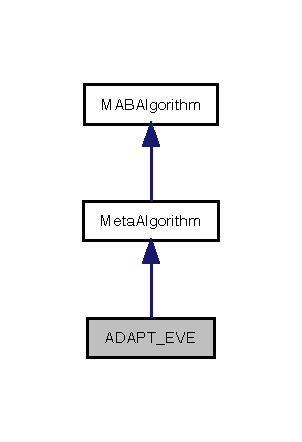
\includegraphics[width=145pt]{class_a_d_a_p_t___e_v_e__inherit__graph}
\end{center}
\end{figure}


Collaboration diagram for A\+D\+A\+P\+T\+\_\+\+E\+VE\+:
\nopagebreak
\begin{figure}[H]
\begin{center}
\leavevmode
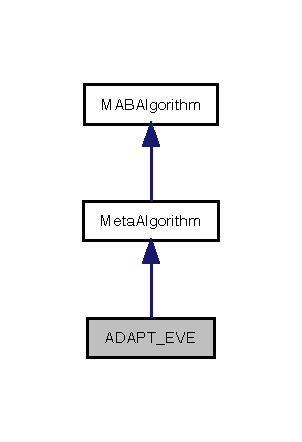
\includegraphics[width=145pt]{class_a_d_a_p_t___e_v_e__coll__graph}
\end{center}
\end{figure}
\subsection*{Public Member Functions}
\begin{DoxyCompactItemize}
\item 
\mbox{\hyperlink{class_a_d_a_p_t___e_v_e_a81ea2b56ec21016d72e621fbd52a8ae0}{A\+D\+A\+P\+T\+\_\+\+E\+VE}} (string \mbox{\hyperlink{class_m_a_b_algorithm_a77b10ecc4b49d519c557f65358167b82}{name}}, int \mbox{\hyperlink{class_m_a_b_algorithm_a340fa9e83e85b092f2c6125fc4e8549b}{num\+\_\+of\+\_\+arms}}, int meta\+\_\+duration, string cdt\+\_\+line, string sub\+\_\+alg\+\_\+line, boost\+::mt19937 \&rng)
\item 
virtual int \mbox{\hyperlink{class_a_d_a_p_t___e_v_e_aa878cacd23fbe8743493623f8a9be6d6}{choose\+\_\+action}} () override
\item 
virtual void \mbox{\hyperlink{class_a_d_a_p_t___e_v_e_ab626b3d8e8f27200e35a0fc3c80f9539}{receive\+\_\+reward}} (double reward, int pulled\+\_\+arm) override
\begin{DoxyCompactList}\small\item\em Update the internal variables of the algorithm according to the new received reward. \end{DoxyCompactList}\item 
virtual void \mbox{\hyperlink{class_a_d_a_p_t___e_v_e_aa89f094cbcba01accada672f0924a5f3}{reset}} (int action=-\/1) override
\begin{DoxyCompactList}\small\item\em resets the internal variables of the algorithm \end{DoxyCompactList}\end{DoxyCompactItemize}
\subsection*{Additional Inherited Members}


\subsection{Detailed Description}
Meta-\/algorithm that couples a sub-\/algorithm with a \mbox{\hyperlink{class_c_d_t}{C\+DT}} for each arm. When a \mbox{\hyperlink{class_c_d_t}{C\+DT}} signals an alarm, the algorithm instantiate a meta-\/bandit setting\+: a new mab with two choices is created, where one choice is using the sub-\/algorithm completely reset and the other choice is using the old sub-\/algorithm. After a certain number of timesteps, the choice with highest mean reward is selected as the new mab and the C\+D\+Ts start monitoring from scratch. 

\subsection{Constructor \& Destructor Documentation}
\mbox{\Hypertarget{class_a_d_a_p_t___e_v_e_a81ea2b56ec21016d72e621fbd52a8ae0}\label{class_a_d_a_p_t___e_v_e_a81ea2b56ec21016d72e621fbd52a8ae0}} 
\index{A\+D\+A\+P\+T\+\_\+\+E\+VE@{A\+D\+A\+P\+T\+\_\+\+E\+VE}!A\+D\+A\+P\+T\+\_\+\+E\+VE@{A\+D\+A\+P\+T\+\_\+\+E\+VE}}
\index{A\+D\+A\+P\+T\+\_\+\+E\+VE@{A\+D\+A\+P\+T\+\_\+\+E\+VE}!A\+D\+A\+P\+T\+\_\+\+E\+VE@{A\+D\+A\+P\+T\+\_\+\+E\+VE}}
\subsubsection{\texorpdfstring{A\+D\+A\+P\+T\+\_\+\+E\+V\+E()}{ADAPT\_EVE()}}
{\footnotesize\ttfamily A\+D\+A\+P\+T\+\_\+\+E\+V\+E\+::\+A\+D\+A\+P\+T\+\_\+\+E\+VE (\begin{DoxyParamCaption}\item[{string}]{name,  }\item[{int}]{num\+\_\+of\+\_\+arms,  }\item[{int}]{meta\+\_\+duration,  }\item[{string}]{cdt\+\_\+line,  }\item[{string}]{sub\+\_\+alg\+\_\+line,  }\item[{boost\+::mt19937 \&}]{rng }\end{DoxyParamCaption})}


\begin{DoxyParams}{Parameters}
{\em name} & string, id of the algorithm \\
\hline
{\em num\+\_\+of\+\_\+arms} & integer, number of arms the algorithm will work with \\
\hline
{\em meta\+\_\+duration} & integer, number of timesteps for the duration of the meta-\/bandit \\
\hline
{\em cdt\+\_\+line} & string, specification of the \mbox{\hyperlink{class_c_d_t}{C\+DT}} \\
\hline
{\em sub\+\_\+alg\+\_\+line} & string, specification of the sub-\/algorithm \\
\hline
{\em rng} & boost\+::mt19937\&, random number generator \\
\hline
\end{DoxyParams}


\subsection{Member Function Documentation}
\mbox{\Hypertarget{class_a_d_a_p_t___e_v_e_aa878cacd23fbe8743493623f8a9be6d6}\label{class_a_d_a_p_t___e_v_e_aa878cacd23fbe8743493623f8a9be6d6}} 
\index{A\+D\+A\+P\+T\+\_\+\+E\+VE@{A\+D\+A\+P\+T\+\_\+\+E\+VE}!choose\+\_\+action@{choose\+\_\+action}}
\index{choose\+\_\+action@{choose\+\_\+action}!A\+D\+A\+P\+T\+\_\+\+E\+VE@{A\+D\+A\+P\+T\+\_\+\+E\+VE}}
\subsubsection{\texorpdfstring{choose\+\_\+action()}{choose\_action()}}
{\footnotesize\ttfamily int A\+D\+A\+P\+T\+\_\+\+E\+V\+E\+::choose\+\_\+action (\begin{DoxyParamCaption}{ }\end{DoxyParamCaption})\hspace{0.3cm}{\ttfamily [override]}, {\ttfamily [virtual]}}

\begin{DoxyReturn}{Returns}
an integer representing the chosen arm 
\end{DoxyReturn}


Implements \mbox{\hyperlink{class_m_a_b_algorithm_afb48f01df0e1860d19759f6e20335007}{M\+A\+B\+Algorithm}}.

\mbox{\Hypertarget{class_a_d_a_p_t___e_v_e_ab626b3d8e8f27200e35a0fc3c80f9539}\label{class_a_d_a_p_t___e_v_e_ab626b3d8e8f27200e35a0fc3c80f9539}} 
\index{A\+D\+A\+P\+T\+\_\+\+E\+VE@{A\+D\+A\+P\+T\+\_\+\+E\+VE}!receive\+\_\+reward@{receive\+\_\+reward}}
\index{receive\+\_\+reward@{receive\+\_\+reward}!A\+D\+A\+P\+T\+\_\+\+E\+VE@{A\+D\+A\+P\+T\+\_\+\+E\+VE}}
\subsubsection{\texorpdfstring{receive\+\_\+reward()}{receive\_reward()}}
{\footnotesize\ttfamily void A\+D\+A\+P\+T\+\_\+\+E\+V\+E\+::receive\+\_\+reward (\begin{DoxyParamCaption}\item[{double}]{reward,  }\item[{int}]{pulled\+\_\+arm }\end{DoxyParamCaption})\hspace{0.3cm}{\ttfamily [override]}, {\ttfamily [virtual]}}



Update the internal variables of the algorithm according to the new received reward. 


\begin{DoxyParams}{Parameters}
{\em reward} & double, new received reward \\
\hline
{\em pulled\+\_\+arm} & integer, represents the pulled arm \\
\hline
\end{DoxyParams}


Reimplemented from \mbox{\hyperlink{class_m_a_b_algorithm_aa584b3d6b86fa050e3389be9781b5782}{M\+A\+B\+Algorithm}}.

\mbox{\Hypertarget{class_a_d_a_p_t___e_v_e_aa89f094cbcba01accada672f0924a5f3}\label{class_a_d_a_p_t___e_v_e_aa89f094cbcba01accada672f0924a5f3}} 
\index{A\+D\+A\+P\+T\+\_\+\+E\+VE@{A\+D\+A\+P\+T\+\_\+\+E\+VE}!reset@{reset}}
\index{reset@{reset}!A\+D\+A\+P\+T\+\_\+\+E\+VE@{A\+D\+A\+P\+T\+\_\+\+E\+VE}}
\subsubsection{\texorpdfstring{reset()}{reset()}}
{\footnotesize\ttfamily void A\+D\+A\+P\+T\+\_\+\+E\+V\+E\+::reset (\begin{DoxyParamCaption}\item[{int}]{action = {\ttfamily -\/1} }\end{DoxyParamCaption})\hspace{0.3cm}{\ttfamily [override]}, {\ttfamily [virtual]}}



resets the internal variables of the algorithm 


\begin{DoxyParams}{Parameters}
{\em action} & integer, specifies which variables to reset. If in (0, num\+\_\+of\+\_\+arms -\/ 1), then it resets only the info related to such arm. If == -\/1, resets all the arms. \\
\hline
\end{DoxyParams}


Reimplemented from \mbox{\hyperlink{class_m_a_b_algorithm_ad5761cee0b0e3421d1f043dbcc0b5f85}{M\+A\+B\+Algorithm}}.



The documentation for this class was generated from the following files\+:\begin{DoxyCompactItemize}
\item 
src/\mbox{\hyperlink{meta__algorithms_8h}{meta\+\_\+algorithms.\+h}}\item 
src/\mbox{\hyperlink{meta__algorithms_8cpp}{meta\+\_\+algorithms.\+cpp}}\end{DoxyCompactItemize}

\hypertarget{class_algorithm___with___uniform___exploration}{}\section{Algorithm\+\_\+\+With\+\_\+\+Uniform\+\_\+\+Exploration Class Reference}
\label{class_algorithm___with___uniform___exploration}\index{Algorithm\+\_\+\+With\+\_\+\+Uniform\+\_\+\+Exploration@{Algorithm\+\_\+\+With\+\_\+\+Uniform\+\_\+\+Exploration}}


Meta-\/algorithm that couples a sub-\/algorithm with uniform exploration over the arms.  




{\ttfamily \#include $<$meta\+\_\+algorithms.\+h$>$}



Inheritance diagram for Algorithm\+\_\+\+With\+\_\+\+Uniform\+\_\+\+Exploration\+:
\nopagebreak
\begin{figure}[H]
\begin{center}
\leavevmode
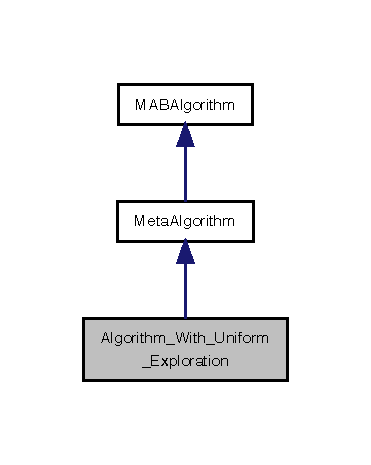
\includegraphics[width=178pt]{class_algorithm___with___uniform___exploration__inherit__graph}
\end{center}
\end{figure}


Collaboration diagram for Algorithm\+\_\+\+With\+\_\+\+Uniform\+\_\+\+Exploration\+:
\nopagebreak
\begin{figure}[H]
\begin{center}
\leavevmode
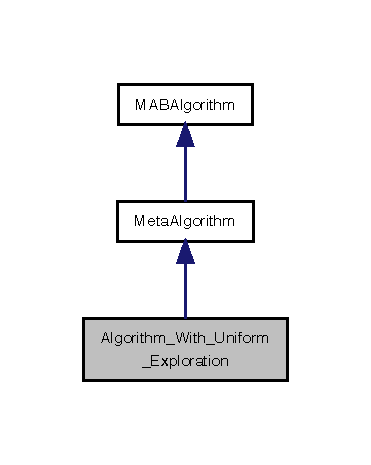
\includegraphics[width=178pt]{class_algorithm___with___uniform___exploration__coll__graph}
\end{center}
\end{figure}
\subsection*{Public Member Functions}
\begin{DoxyCompactItemize}
\item 
\mbox{\hyperlink{class_algorithm___with___uniform___exploration_accc377b55bd1d48b9cfa1ce952ff3cf8}{Algorithm\+\_\+\+With\+\_\+\+Uniform\+\_\+\+Exploration}} (string \mbox{\hyperlink{class_m_a_b_algorithm_a77b10ecc4b49d519c557f65358167b82}{name}}, int \mbox{\hyperlink{class_m_a_b_algorithm_a340fa9e83e85b092f2c6125fc4e8549b}{num\+\_\+of\+\_\+arms}}, string sub\+\_\+alg\+\_\+line, double alpha, boost\+::mt19937 \&rng)
\item 
virtual int \mbox{\hyperlink{class_algorithm___with___uniform___exploration_a42d5f75def328c83dce00f73dbe26d58}{choose\+\_\+action}} () override
\item 
virtual void \mbox{\hyperlink{class_algorithm___with___uniform___exploration_a946808f681cd7b54bd557e1d8f15c5d0}{receive\+\_\+reward}} (double reward, int pulled\+\_\+arm) override
\begin{DoxyCompactList}\small\item\em Update the internal variables of the algorithm according to the new received reward. \end{DoxyCompactList}\item 
virtual void \mbox{\hyperlink{class_algorithm___with___uniform___exploration_a96b0df2a59099ba8b4cc83f21b407642}{reset}} (int action=-\/1) override
\begin{DoxyCompactList}\small\item\em resets the internal variables of the algorithm \end{DoxyCompactList}\end{DoxyCompactItemize}
\subsection*{Additional Inherited Members}


\subsection{Detailed Description}
Meta-\/algorithm that couples a sub-\/algorithm with uniform exploration over the arms. 

\subsection{Constructor \& Destructor Documentation}
\mbox{\Hypertarget{class_algorithm___with___uniform___exploration_accc377b55bd1d48b9cfa1ce952ff3cf8}\label{class_algorithm___with___uniform___exploration_accc377b55bd1d48b9cfa1ce952ff3cf8}} 
\index{Algorithm\+\_\+\+With\+\_\+\+Uniform\+\_\+\+Exploration@{Algorithm\+\_\+\+With\+\_\+\+Uniform\+\_\+\+Exploration}!Algorithm\+\_\+\+With\+\_\+\+Uniform\+\_\+\+Exploration@{Algorithm\+\_\+\+With\+\_\+\+Uniform\+\_\+\+Exploration}}
\index{Algorithm\+\_\+\+With\+\_\+\+Uniform\+\_\+\+Exploration@{Algorithm\+\_\+\+With\+\_\+\+Uniform\+\_\+\+Exploration}!Algorithm\+\_\+\+With\+\_\+\+Uniform\+\_\+\+Exploration@{Algorithm\+\_\+\+With\+\_\+\+Uniform\+\_\+\+Exploration}}
\subsubsection{\texorpdfstring{Algorithm\+\_\+\+With\+\_\+\+Uniform\+\_\+\+Exploration()}{Algorithm\_With\_Uniform\_Exploration()}}
{\footnotesize\ttfamily Algorithm\+\_\+\+With\+\_\+\+Uniform\+\_\+\+Exploration\+::\+Algorithm\+\_\+\+With\+\_\+\+Uniform\+\_\+\+Exploration (\begin{DoxyParamCaption}\item[{string}]{name,  }\item[{int}]{num\+\_\+of\+\_\+arms,  }\item[{string}]{sub\+\_\+alg\+\_\+line,  }\item[{double}]{alpha,  }\item[{boost\+::mt19937 \&}]{rng }\end{DoxyParamCaption})}


\begin{DoxyParams}{Parameters}
{\em name} & string, id of the algorithm \\
\hline
{\em num\+\_\+of\+\_\+arms} & integer, number of arms the algorithm will work with \\
\hline
{\em sub\+\_\+alg\+\_\+line} & string, specification of the sub-\/algorithm \\
\hline
{\em alpha} & double in (0,1), exploration parameter \\
\hline
{\em rng} & boost\+::mt19937\&, random number generator \\
\hline
\end{DoxyParams}


\subsection{Member Function Documentation}
\mbox{\Hypertarget{class_algorithm___with___uniform___exploration_a42d5f75def328c83dce00f73dbe26d58}\label{class_algorithm___with___uniform___exploration_a42d5f75def328c83dce00f73dbe26d58}} 
\index{Algorithm\+\_\+\+With\+\_\+\+Uniform\+\_\+\+Exploration@{Algorithm\+\_\+\+With\+\_\+\+Uniform\+\_\+\+Exploration}!choose\+\_\+action@{choose\+\_\+action}}
\index{choose\+\_\+action@{choose\+\_\+action}!Algorithm\+\_\+\+With\+\_\+\+Uniform\+\_\+\+Exploration@{Algorithm\+\_\+\+With\+\_\+\+Uniform\+\_\+\+Exploration}}
\subsubsection{\texorpdfstring{choose\+\_\+action()}{choose\_action()}}
{\footnotesize\ttfamily int Algorithm\+\_\+\+With\+\_\+\+Uniform\+\_\+\+Exploration\+::choose\+\_\+action (\begin{DoxyParamCaption}{ }\end{DoxyParamCaption})\hspace{0.3cm}{\ttfamily [override]}, {\ttfamily [virtual]}}

\begin{DoxyReturn}{Returns}
an integer representing the chosen arm 
\end{DoxyReturn}


Implements \mbox{\hyperlink{class_m_a_b_algorithm_afb48f01df0e1860d19759f6e20335007}{M\+A\+B\+Algorithm}}.

\mbox{\Hypertarget{class_algorithm___with___uniform___exploration_a946808f681cd7b54bd557e1d8f15c5d0}\label{class_algorithm___with___uniform___exploration_a946808f681cd7b54bd557e1d8f15c5d0}} 
\index{Algorithm\+\_\+\+With\+\_\+\+Uniform\+\_\+\+Exploration@{Algorithm\+\_\+\+With\+\_\+\+Uniform\+\_\+\+Exploration}!receive\+\_\+reward@{receive\+\_\+reward}}
\index{receive\+\_\+reward@{receive\+\_\+reward}!Algorithm\+\_\+\+With\+\_\+\+Uniform\+\_\+\+Exploration@{Algorithm\+\_\+\+With\+\_\+\+Uniform\+\_\+\+Exploration}}
\subsubsection{\texorpdfstring{receive\+\_\+reward()}{receive\_reward()}}
{\footnotesize\ttfamily void Algorithm\+\_\+\+With\+\_\+\+Uniform\+\_\+\+Exploration\+::receive\+\_\+reward (\begin{DoxyParamCaption}\item[{double}]{reward,  }\item[{int}]{pulled\+\_\+arm }\end{DoxyParamCaption})\hspace{0.3cm}{\ttfamily [override]}, {\ttfamily [virtual]}}



Update the internal variables of the algorithm according to the new received reward. 


\begin{DoxyParams}{Parameters}
{\em reward} & double, new received reward \\
\hline
{\em pulled\+\_\+arm} & integer, represents the pulled arm \\
\hline
\end{DoxyParams}


Reimplemented from \mbox{\hyperlink{class_m_a_b_algorithm_aa584b3d6b86fa050e3389be9781b5782}{M\+A\+B\+Algorithm}}.

\mbox{\Hypertarget{class_algorithm___with___uniform___exploration_a96b0df2a59099ba8b4cc83f21b407642}\label{class_algorithm___with___uniform___exploration_a96b0df2a59099ba8b4cc83f21b407642}} 
\index{Algorithm\+\_\+\+With\+\_\+\+Uniform\+\_\+\+Exploration@{Algorithm\+\_\+\+With\+\_\+\+Uniform\+\_\+\+Exploration}!reset@{reset}}
\index{reset@{reset}!Algorithm\+\_\+\+With\+\_\+\+Uniform\+\_\+\+Exploration@{Algorithm\+\_\+\+With\+\_\+\+Uniform\+\_\+\+Exploration}}
\subsubsection{\texorpdfstring{reset()}{reset()}}
{\footnotesize\ttfamily void Algorithm\+\_\+\+With\+\_\+\+Uniform\+\_\+\+Exploration\+::reset (\begin{DoxyParamCaption}\item[{int}]{action = {\ttfamily -\/1} }\end{DoxyParamCaption})\hspace{0.3cm}{\ttfamily [override]}, {\ttfamily [virtual]}}



resets the internal variables of the algorithm 


\begin{DoxyParams}{Parameters}
{\em action} & integer, specifies which variables to reset. If in (0, num\+\_\+of\+\_\+arms -\/ 1), then it resets only the info related to such arm. If == -\/1, resets all the arms. \\
\hline
\end{DoxyParams}


Reimplemented from \mbox{\hyperlink{class_m_a_b_algorithm_ad5761cee0b0e3421d1f043dbcc0b5f85}{M\+A\+B\+Algorithm}}.



The documentation for this class was generated from the following files\+:\begin{DoxyCompactItemize}
\item 
src/\mbox{\hyperlink{meta__algorithms_8h}{meta\+\_\+algorithms.\+h}}\item 
src/\mbox{\hyperlink{meta__algorithms_8cpp}{meta\+\_\+algorithms.\+cpp}}\end{DoxyCompactItemize}

\hypertarget{class_bernoulli_distribution}{}\section{Bernoulli\+Distribution Class Reference}
\label{class_bernoulli_distribution}\index{Bernoulli\+Distribution@{Bernoulli\+Distribution}}


\mbox{\hyperlink{class_distribution}{Distribution}} of a bernoulli distribution.  




{\ttfamily \#include $<$distribution.\+h$>$}



Inheritance diagram for Bernoulli\+Distribution\+:
\nopagebreak
\begin{figure}[H]
\begin{center}
\leavevmode
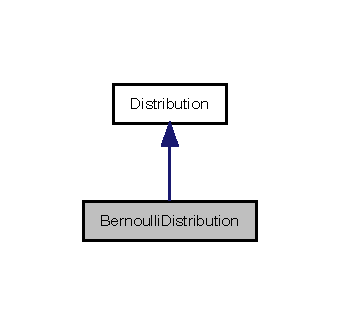
\includegraphics[width=163pt]{class_bernoulli_distribution__inherit__graph}
\end{center}
\end{figure}


Collaboration diagram for Bernoulli\+Distribution\+:
\nopagebreak
\begin{figure}[H]
\begin{center}
\leavevmode
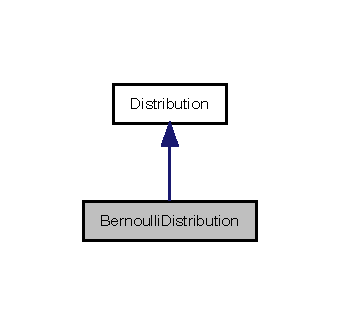
\includegraphics[width=163pt]{class_bernoulli_distribution__coll__graph}
\end{center}
\end{figure}
\subsection*{Public Member Functions}
\begin{DoxyCompactItemize}
\item 
\mbox{\hyperlink{class_bernoulli_distribution_af67a1f09e36a64d7fd5a14476d24785c}{Bernoulli\+Distribution}} (string \mbox{\hyperlink{class_distribution_ab3b7be02f0401cb76beb2e744b6161f9}{name}}, double p, boost\+::mt19937 \&\mbox{\hyperlink{class_distribution_ac8915a45ce85ab6b7506fa42bb850a89}{rng}})
\item 
double \mbox{\hyperlink{class_bernoulli_distribution_ae733579a1c78c01ba8d915bfb8d7b088}{draw}} (int timestep) override
\item 
string \mbox{\hyperlink{class_bernoulli_distribution_a29f9f1014234828255def7bf9872b086}{to\+File}} () override
\begin{DoxyCompactList}\small\item\em build a representation of this \mbox{\hyperlink{class_distribution}{Distribution}} so that it can be printed to a file and be later analysed by another script \end{DoxyCompactList}\item 
double \mbox{\hyperlink{class_bernoulli_distribution_a7756a9b4861bf90bc7cc346e77b40603}{get\+\_\+mean}} (int timestep) override
\end{DoxyCompactItemize}
\subsection*{Additional Inherited Members}


\subsection{Detailed Description}
\mbox{\hyperlink{class_distribution}{Distribution}} of a bernoulli distribution. 


\begin{DoxyParams}{Parameters}
{\em name} & string, id of the distribution \\
\hline
{\em p} & double, probability of obtaining 1 from the bernoulli distribution \\
\hline
{\em rng} & boost\+::mt19937\&, rng used to generate data \\
\hline
\end{DoxyParams}


\subsection{Constructor \& Destructor Documentation}
\mbox{\Hypertarget{class_bernoulli_distribution_af67a1f09e36a64d7fd5a14476d24785c}\label{class_bernoulli_distribution_af67a1f09e36a64d7fd5a14476d24785c}} 
\index{Bernoulli\+Distribution@{Bernoulli\+Distribution}!Bernoulli\+Distribution@{Bernoulli\+Distribution}}
\index{Bernoulli\+Distribution@{Bernoulli\+Distribution}!Bernoulli\+Distribution@{Bernoulli\+Distribution}}
\subsubsection{\texorpdfstring{Bernoulli\+Distribution()}{BernoulliDistribution()}}
{\footnotesize\ttfamily Bernoulli\+Distribution\+::\+Bernoulli\+Distribution (\begin{DoxyParamCaption}\item[{string}]{name,  }\item[{double}]{p,  }\item[{boost\+::mt19937 \&}]{rng }\end{DoxyParamCaption})}


\begin{DoxyParams}{Parameters}
{\em name} & string, id of the distribution \\
\hline
{\em p} & double, probability of obtaining 1 from the bernoulli distribution \\
\hline
{\em rng} & boost\+::mt19937\&, rng used to generate data \\
\hline
\end{DoxyParams}


\subsection{Member Function Documentation}
\mbox{\Hypertarget{class_bernoulli_distribution_ae733579a1c78c01ba8d915bfb8d7b088}\label{class_bernoulli_distribution_ae733579a1c78c01ba8d915bfb8d7b088}} 
\index{Bernoulli\+Distribution@{Bernoulli\+Distribution}!draw@{draw}}
\index{draw@{draw}!Bernoulli\+Distribution@{Bernoulli\+Distribution}}
\subsubsection{\texorpdfstring{draw()}{draw()}}
{\footnotesize\ttfamily double Bernoulli\+Distribution\+::draw (\begin{DoxyParamCaption}\item[{int}]{timestep }\end{DoxyParamCaption})\hspace{0.3cm}{\ttfamily [override]}, {\ttfamily [virtual]}}


\begin{DoxyParams}{Parameters}
{\em timestep} & int, timestep at which the reward is drawn \\
\hline
\end{DoxyParams}
\begin{DoxyReturn}{Returns}
a double which is the drawn reward 
\end{DoxyReturn}


Implements \mbox{\hyperlink{class_distribution_a742b398af4a461243028cce3c47d8080}{Distribution}}.

\mbox{\Hypertarget{class_bernoulli_distribution_a7756a9b4861bf90bc7cc346e77b40603}\label{class_bernoulli_distribution_a7756a9b4861bf90bc7cc346e77b40603}} 
\index{Bernoulli\+Distribution@{Bernoulli\+Distribution}!get\+\_\+mean@{get\+\_\+mean}}
\index{get\+\_\+mean@{get\+\_\+mean}!Bernoulli\+Distribution@{Bernoulli\+Distribution}}
\subsubsection{\texorpdfstring{get\+\_\+mean()}{get\_mean()}}
{\footnotesize\ttfamily double Bernoulli\+Distribution\+::get\+\_\+mean (\begin{DoxyParamCaption}\item[{int}]{timestep }\end{DoxyParamCaption})\hspace{0.3cm}{\ttfamily [override]}, {\ttfamily [virtual]}}


\begin{DoxyParams}{Parameters}
{\em timestep} & integer, the timestep at which the mean is asked \\
\hline
\end{DoxyParams}
\begin{DoxyReturn}{Returns}
the mean (double) at the specified timestep 
\end{DoxyReturn}


Implements \mbox{\hyperlink{class_distribution_ac9c74d18549f532caa09ae86d8b25b55}{Distribution}}.

\mbox{\Hypertarget{class_bernoulli_distribution_a29f9f1014234828255def7bf9872b086}\label{class_bernoulli_distribution_a29f9f1014234828255def7bf9872b086}} 
\index{Bernoulli\+Distribution@{Bernoulli\+Distribution}!to\+File@{to\+File}}
\index{to\+File@{to\+File}!Bernoulli\+Distribution@{Bernoulli\+Distribution}}
\subsubsection{\texorpdfstring{to\+File()}{toFile()}}
{\footnotesize\ttfamily string Bernoulli\+Distribution\+::to\+File (\begin{DoxyParamCaption}{ }\end{DoxyParamCaption})\hspace{0.3cm}{\ttfamily [override]}, {\ttfamily [virtual]}}



build a representation of this \mbox{\hyperlink{class_distribution}{Distribution}} so that it can be printed to a file and be later analysed by another script 

\begin{DoxyReturn}{Returns}
a string that represents this \mbox{\hyperlink{class_distribution}{Distribution}} 
\end{DoxyReturn}


Implements \mbox{\hyperlink{class_distribution_ac41d57a4d7f82041810f886590a236a5}{Distribution}}.



The documentation for this class was generated from the following files\+:\begin{DoxyCompactItemize}
\item 
src/\mbox{\hyperlink{distribution_8h}{distribution.\+h}}\item 
src/\mbox{\hyperlink{distribution_8cpp}{distribution.\+cpp}}\end{DoxyCompactItemize}

\hypertarget{class_bernoulli_non_stationary_distribution}{}\section{Bernoulli\+Non\+Stationary\+Distribution Class Reference}
\label{class_bernoulli_non_stationary_distribution}\index{Bernoulli\+Non\+Stationary\+Distribution@{Bernoulli\+Non\+Stationary\+Distribution}}


\mbox{\hyperlink{class_distribution}{Distribution}} of a non-\/stationary bernoulli distribution.  




{\ttfamily \#include $<$distribution.\+h$>$}



Inheritance diagram for Bernoulli\+Non\+Stationary\+Distribution\+:
\nopagebreak
\begin{figure}[H]
\begin{center}
\leavevmode
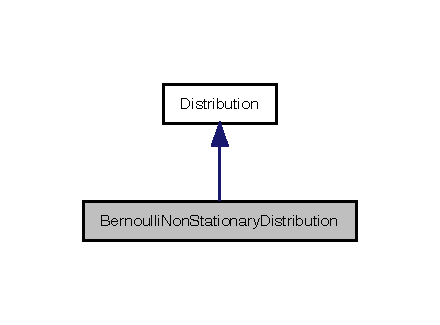
\includegraphics[width=211pt]{class_bernoulli_non_stationary_distribution__inherit__graph}
\end{center}
\end{figure}


Collaboration diagram for Bernoulli\+Non\+Stationary\+Distribution\+:
\nopagebreak
\begin{figure}[H]
\begin{center}
\leavevmode
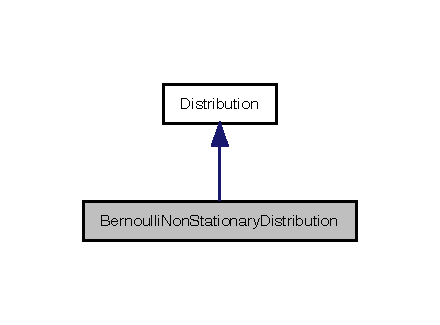
\includegraphics[width=211pt]{class_bernoulli_non_stationary_distribution__coll__graph}
\end{center}
\end{figure}
\subsection*{Public Member Functions}
\begin{DoxyCompactItemize}
\item 
\mbox{\hyperlink{class_bernoulli_non_stationary_distribution_a518c66c5e7f3f12712a29c6e4b6d9b2e}{Bernoulli\+Non\+Stationary\+Distribution}} (string \mbox{\hyperlink{class_distribution_ab3b7be02f0401cb76beb2e744b6161f9}{name}}, vector$<$ double $>$ \&ps, vector$<$ int $>$ \&ends, boost\+::mt19937 \&\mbox{\hyperlink{class_distribution_ac8915a45ce85ab6b7506fa42bb850a89}{rng}})
\item 
double \mbox{\hyperlink{class_bernoulli_non_stationary_distribution_a4aee952b4eebc5d36ff318b4c30f4a5d}{draw}} (int timestep) override
\item 
string \mbox{\hyperlink{class_bernoulli_non_stationary_distribution_a5db3f4675ff988f3c775a939f8ef4847}{to\+File}} () override
\begin{DoxyCompactList}\small\item\em build a representation of this \mbox{\hyperlink{class_distribution}{Distribution}} so that it can be printed to a file and be later analysed by another script \end{DoxyCompactList}\item 
double \mbox{\hyperlink{class_bernoulli_non_stationary_distribution_ab1cf34057259a933b7957fbff28ed442}{get\+\_\+mean}} (int timestep) override
\end{DoxyCompactItemize}
\subsection*{Additional Inherited Members}


\subsection{Detailed Description}
\mbox{\hyperlink{class_distribution}{Distribution}} of a non-\/stationary bernoulli distribution. 


\begin{DoxyParams}{Parameters}
{\em name} & string, id of the distribution \\
\hline
{\em ps} & vector$<$double$>$\&, the probabilities of obtaining 1 from the bernoulli distributions in the time slots \\
\hline
{\em ends} & vector$<$double$>$\&, the last timestep of each time slot \\
\hline
{\em rng} & boost\+::mt19937\&, rng used to generate data \\
\hline
\end{DoxyParams}


\subsection{Constructor \& Destructor Documentation}
\mbox{\Hypertarget{class_bernoulli_non_stationary_distribution_a518c66c5e7f3f12712a29c6e4b6d9b2e}\label{class_bernoulli_non_stationary_distribution_a518c66c5e7f3f12712a29c6e4b6d9b2e}} 
\index{Bernoulli\+Non\+Stationary\+Distribution@{Bernoulli\+Non\+Stationary\+Distribution}!Bernoulli\+Non\+Stationary\+Distribution@{Bernoulli\+Non\+Stationary\+Distribution}}
\index{Bernoulli\+Non\+Stationary\+Distribution@{Bernoulli\+Non\+Stationary\+Distribution}!Bernoulli\+Non\+Stationary\+Distribution@{Bernoulli\+Non\+Stationary\+Distribution}}
\subsubsection{\texorpdfstring{Bernoulli\+Non\+Stationary\+Distribution()}{BernoulliNonStationaryDistribution()}}
{\footnotesize\ttfamily Bernoulli\+Non\+Stationary\+Distribution\+::\+Bernoulli\+Non\+Stationary\+Distribution (\begin{DoxyParamCaption}\item[{string}]{name,  }\item[{vector$<$ double $>$ \&}]{ps,  }\item[{vector$<$ int $>$ \&}]{ends,  }\item[{boost\+::mt19937 \&}]{rng }\end{DoxyParamCaption})}


\begin{DoxyParams}{Parameters}
{\em name} & string, id of the distribution \\
\hline
{\em ps} & vector$<$double$>$\&, the probabilities of obtaining 1 from the bernoulli distributions in the time slots \\
\hline
{\em ends} & vector$<$double$>$\&, the last timestep of each time slot \\
\hline
{\em rng} & boost\+::mt19937\&, rng used to generate data \\
\hline
\end{DoxyParams}


\subsection{Member Function Documentation}
\mbox{\Hypertarget{class_bernoulli_non_stationary_distribution_a4aee952b4eebc5d36ff318b4c30f4a5d}\label{class_bernoulli_non_stationary_distribution_a4aee952b4eebc5d36ff318b4c30f4a5d}} 
\index{Bernoulli\+Non\+Stationary\+Distribution@{Bernoulli\+Non\+Stationary\+Distribution}!draw@{draw}}
\index{draw@{draw}!Bernoulli\+Non\+Stationary\+Distribution@{Bernoulli\+Non\+Stationary\+Distribution}}
\subsubsection{\texorpdfstring{draw()}{draw()}}
{\footnotesize\ttfamily double Bernoulli\+Non\+Stationary\+Distribution\+::draw (\begin{DoxyParamCaption}\item[{int}]{timestep }\end{DoxyParamCaption})\hspace{0.3cm}{\ttfamily [override]}, {\ttfamily [virtual]}}


\begin{DoxyParams}{Parameters}
{\em timestep} & int, timestep at which the reward is drawn \\
\hline
\end{DoxyParams}
\begin{DoxyReturn}{Returns}
a double which is the drawn reward 
\end{DoxyReturn}


Implements \mbox{\hyperlink{class_distribution_a742b398af4a461243028cce3c47d8080}{Distribution}}.

\mbox{\Hypertarget{class_bernoulli_non_stationary_distribution_ab1cf34057259a933b7957fbff28ed442}\label{class_bernoulli_non_stationary_distribution_ab1cf34057259a933b7957fbff28ed442}} 
\index{Bernoulli\+Non\+Stationary\+Distribution@{Bernoulli\+Non\+Stationary\+Distribution}!get\+\_\+mean@{get\+\_\+mean}}
\index{get\+\_\+mean@{get\+\_\+mean}!Bernoulli\+Non\+Stationary\+Distribution@{Bernoulli\+Non\+Stationary\+Distribution}}
\subsubsection{\texorpdfstring{get\+\_\+mean()}{get\_mean()}}
{\footnotesize\ttfamily double Bernoulli\+Non\+Stationary\+Distribution\+::get\+\_\+mean (\begin{DoxyParamCaption}\item[{int}]{timestep }\end{DoxyParamCaption})\hspace{0.3cm}{\ttfamily [override]}, {\ttfamily [virtual]}}


\begin{DoxyParams}{Parameters}
{\em timestep} & integer, the timestep at which the mean is asked \\
\hline
\end{DoxyParams}
\begin{DoxyReturn}{Returns}
the mean (double) at the specified timestep 
\end{DoxyReturn}


Implements \mbox{\hyperlink{class_distribution_ac9c74d18549f532caa09ae86d8b25b55}{Distribution}}.

\mbox{\Hypertarget{class_bernoulli_non_stationary_distribution_a5db3f4675ff988f3c775a939f8ef4847}\label{class_bernoulli_non_stationary_distribution_a5db3f4675ff988f3c775a939f8ef4847}} 
\index{Bernoulli\+Non\+Stationary\+Distribution@{Bernoulli\+Non\+Stationary\+Distribution}!to\+File@{to\+File}}
\index{to\+File@{to\+File}!Bernoulli\+Non\+Stationary\+Distribution@{Bernoulli\+Non\+Stationary\+Distribution}}
\subsubsection{\texorpdfstring{to\+File()}{toFile()}}
{\footnotesize\ttfamily string Bernoulli\+Non\+Stationary\+Distribution\+::to\+File (\begin{DoxyParamCaption}{ }\end{DoxyParamCaption})\hspace{0.3cm}{\ttfamily [override]}, {\ttfamily [virtual]}}



build a representation of this \mbox{\hyperlink{class_distribution}{Distribution}} so that it can be printed to a file and be later analysed by another script 

\begin{DoxyReturn}{Returns}
a string that represents this \mbox{\hyperlink{class_distribution}{Distribution}} 
\end{DoxyReturn}


Implements \mbox{\hyperlink{class_distribution_ac41d57a4d7f82041810f886590a236a5}{Distribution}}.



The documentation for this class was generated from the following files\+:\begin{DoxyCompactItemize}
\item 
src/\mbox{\hyperlink{distribution_8h}{distribution.\+h}}\item 
src/\mbox{\hyperlink{distribution_8cpp}{distribution.\+cpp}}\end{DoxyCompactItemize}

\hypertarget{class_c_d___algorithm}{}\section{C\+D\+\_\+\+Algorithm Class Reference}
\label{class_c_d___algorithm}\index{C\+D\+\_\+\+Algorithm@{C\+D\+\_\+\+Algorithm}}


Meta-\/algorithm that couples a sub-\/algorithm with a change detection test for each arm. When a \mbox{\hyperlink{class_c_d_t}{C\+DT}} signals an alarm, the info about the corresponding arm is reset on the sub-\/algorithm.  




{\ttfamily \#include $<$meta\+\_\+algorithms.\+h$>$}



Inheritance diagram for C\+D\+\_\+\+Algorithm\+:
\nopagebreak
\begin{figure}[H]
\begin{center}
\leavevmode
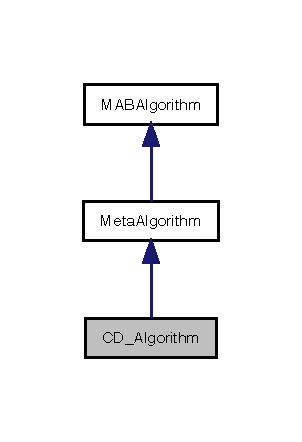
\includegraphics[width=145pt]{class_c_d___algorithm__inherit__graph}
\end{center}
\end{figure}


Collaboration diagram for C\+D\+\_\+\+Algorithm\+:
\nopagebreak
\begin{figure}[H]
\begin{center}
\leavevmode
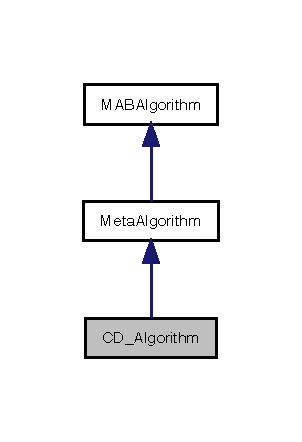
\includegraphics[width=145pt]{class_c_d___algorithm__coll__graph}
\end{center}
\end{figure}
\subsection*{Public Member Functions}
\begin{DoxyCompactItemize}
\item 
\mbox{\hyperlink{class_c_d___algorithm_a3fcecaa468fa082e20461c53ab366550}{C\+D\+\_\+\+Algorithm}} (string \mbox{\hyperlink{class_m_a_b_algorithm_a77b10ecc4b49d519c557f65358167b82}{name}}, int \mbox{\hyperlink{class_m_a_b_algorithm_a340fa9e83e85b092f2c6125fc4e8549b}{num\+\_\+of\+\_\+arms}}, int M, string cdt\+\_\+line, string sub\+\_\+alg\+\_\+line, bool use\+\_\+history, int max\+\_\+history, boost\+::mt19937 \&rng)
\item 
virtual int \mbox{\hyperlink{class_c_d___algorithm_a10d80cbf4687e2c0ef69466ee6deb1a9}{choose\+\_\+action}} () override
\item 
virtual void \mbox{\hyperlink{class_c_d___algorithm_a2427ddf68550eda00a0992b875c10834}{receive\+\_\+reward}} (double reward, int pulled\+\_\+arm) override
\begin{DoxyCompactList}\small\item\em Update the internal variables of the algorithm according to the new received reward. \end{DoxyCompactList}\item 
virtual void \mbox{\hyperlink{class_c_d___algorithm_a493e6eaafb4ab105c94e9e4c33143d39}{reset}} (int action=-\/1) override
\begin{DoxyCompactList}\small\item\em resets the internal variables of the algorithm \end{DoxyCompactList}\end{DoxyCompactItemize}
\subsection*{Additional Inherited Members}


\subsection{Detailed Description}
Meta-\/algorithm that couples a sub-\/algorithm with a change detection test for each arm. When a \mbox{\hyperlink{class_c_d_t}{C\+DT}} signals an alarm, the info about the corresponding arm is reset on the sub-\/algorithm. 

\subsection{Constructor \& Destructor Documentation}
\mbox{\Hypertarget{class_c_d___algorithm_a3fcecaa468fa082e20461c53ab366550}\label{class_c_d___algorithm_a3fcecaa468fa082e20461c53ab366550}} 
\index{C\+D\+\_\+\+Algorithm@{C\+D\+\_\+\+Algorithm}!C\+D\+\_\+\+Algorithm@{C\+D\+\_\+\+Algorithm}}
\index{C\+D\+\_\+\+Algorithm@{C\+D\+\_\+\+Algorithm}!C\+D\+\_\+\+Algorithm@{C\+D\+\_\+\+Algorithm}}
\subsubsection{\texorpdfstring{C\+D\+\_\+\+Algorithm()}{CD\_Algorithm()}}
{\footnotesize\ttfamily C\+D\+\_\+\+Algorithm\+::\+C\+D\+\_\+\+Algorithm (\begin{DoxyParamCaption}\item[{string}]{name,  }\item[{int}]{num\+\_\+of\+\_\+arms,  }\item[{int}]{M,  }\item[{string}]{cdt\+\_\+line,  }\item[{string}]{sub\+\_\+alg\+\_\+line,  }\item[{bool}]{use\+\_\+history,  }\item[{int}]{max\+\_\+history,  }\item[{boost\+::mt19937 \&}]{rng }\end{DoxyParamCaption})}


\begin{DoxyParams}{Parameters}
{\em name} & string, id of the algorithm \\
\hline
{\em num\+\_\+of\+\_\+arms} & integer, number of arms the algorithm will work with \\
\hline
{\em M} & integer, number of timesteps required by the \mbox{\hyperlink{class_c_d_t}{C\+DT}} to initialize itself \\
\hline
{\em cdt\+\_\+line} & string, specification of the \mbox{\hyperlink{class_c_d_t}{C\+DT}} \\
\hline
{\em sub\+\_\+alg\+\_\+line} & string, specification of the sub-\/algorithm \\
\hline
{\em use\+\_\+history} & boolean, if true the sub-\/algorithm is not completely reset, and the sample history after the estimated change point is kept in the sub-\/algorithm \\
\hline
{\em max\+\_\+history} & integer, maximum amount of sample history that the algorithm can use \\
\hline
{\em rng} & boost\+::mt19937\&, random number generator \\
\hline
\end{DoxyParams}


\subsection{Member Function Documentation}
\mbox{\Hypertarget{class_c_d___algorithm_a10d80cbf4687e2c0ef69466ee6deb1a9}\label{class_c_d___algorithm_a10d80cbf4687e2c0ef69466ee6deb1a9}} 
\index{C\+D\+\_\+\+Algorithm@{C\+D\+\_\+\+Algorithm}!choose\+\_\+action@{choose\+\_\+action}}
\index{choose\+\_\+action@{choose\+\_\+action}!C\+D\+\_\+\+Algorithm@{C\+D\+\_\+\+Algorithm}}
\subsubsection{\texorpdfstring{choose\+\_\+action()}{choose\_action()}}
{\footnotesize\ttfamily int C\+D\+\_\+\+Algorithm\+::choose\+\_\+action (\begin{DoxyParamCaption}{ }\end{DoxyParamCaption})\hspace{0.3cm}{\ttfamily [override]}, {\ttfamily [virtual]}}

\begin{DoxyReturn}{Returns}
an integer representing the chosen arm 
\end{DoxyReturn}


Implements \mbox{\hyperlink{class_m_a_b_algorithm_afb48f01df0e1860d19759f6e20335007}{M\+A\+B\+Algorithm}}.

\mbox{\Hypertarget{class_c_d___algorithm_a2427ddf68550eda00a0992b875c10834}\label{class_c_d___algorithm_a2427ddf68550eda00a0992b875c10834}} 
\index{C\+D\+\_\+\+Algorithm@{C\+D\+\_\+\+Algorithm}!receive\+\_\+reward@{receive\+\_\+reward}}
\index{receive\+\_\+reward@{receive\+\_\+reward}!C\+D\+\_\+\+Algorithm@{C\+D\+\_\+\+Algorithm}}
\subsubsection{\texorpdfstring{receive\+\_\+reward()}{receive\_reward()}}
{\footnotesize\ttfamily void C\+D\+\_\+\+Algorithm\+::receive\+\_\+reward (\begin{DoxyParamCaption}\item[{double}]{reward,  }\item[{int}]{pulled\+\_\+arm }\end{DoxyParamCaption})\hspace{0.3cm}{\ttfamily [override]}, {\ttfamily [virtual]}}



Update the internal variables of the algorithm according to the new received reward. 


\begin{DoxyParams}{Parameters}
{\em reward} & double, new received reward \\
\hline
{\em pulled\+\_\+arm} & integer, represents the pulled arm \\
\hline
\end{DoxyParams}


Reimplemented from \mbox{\hyperlink{class_m_a_b_algorithm_aa584b3d6b86fa050e3389be9781b5782}{M\+A\+B\+Algorithm}}.

\mbox{\Hypertarget{class_c_d___algorithm_a493e6eaafb4ab105c94e9e4c33143d39}\label{class_c_d___algorithm_a493e6eaafb4ab105c94e9e4c33143d39}} 
\index{C\+D\+\_\+\+Algorithm@{C\+D\+\_\+\+Algorithm}!reset@{reset}}
\index{reset@{reset}!C\+D\+\_\+\+Algorithm@{C\+D\+\_\+\+Algorithm}}
\subsubsection{\texorpdfstring{reset()}{reset()}}
{\footnotesize\ttfamily void C\+D\+\_\+\+Algorithm\+::reset (\begin{DoxyParamCaption}\item[{int}]{action = {\ttfamily -\/1} }\end{DoxyParamCaption})\hspace{0.3cm}{\ttfamily [override]}, {\ttfamily [virtual]}}



resets the internal variables of the algorithm 


\begin{DoxyParams}{Parameters}
{\em action} & integer, specifies which variables to reset. If in (0, num\+\_\+of\+\_\+arms -\/ 1), then it resets only the info related to such arm. If == -\/1, resets all the arms. \\
\hline
\end{DoxyParams}


Reimplemented from \mbox{\hyperlink{class_m_a_b_algorithm_ad5761cee0b0e3421d1f043dbcc0b5f85}{M\+A\+B\+Algorithm}}.



The documentation for this class was generated from the following files\+:\begin{DoxyCompactItemize}
\item 
src/\mbox{\hyperlink{meta__algorithms_8h}{meta\+\_\+algorithms.\+h}}\item 
src/\mbox{\hyperlink{meta__algorithms_8cpp}{meta\+\_\+algorithms.\+cpp}}\end{DoxyCompactItemize}

\hypertarget{class_c_d_t}{}\section{C\+DT Class Reference}
\label{class_c_d_t}\index{C\+DT@{C\+DT}}


Base class of all the \mbox{\hyperlink{class_c_d_t}{C\+DT}} procedures.  




{\ttfamily \#include $<$cdt.\+h$>$}



Inheritance diagram for C\+DT\+:
\nopagebreak
\begin{figure}[H]
\begin{center}
\leavevmode
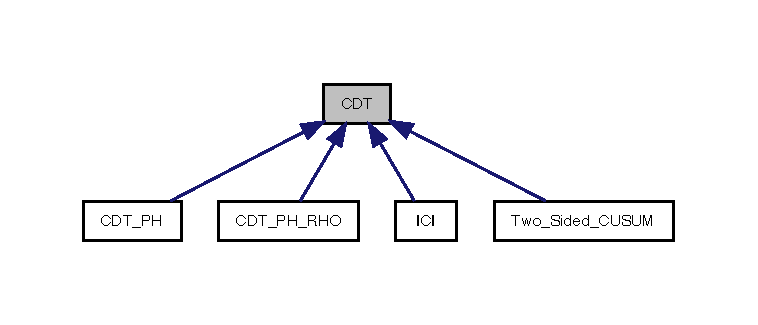
\includegraphics[width=350pt]{class_c_d_t__inherit__graph}
\end{center}
\end{figure}
\subsection*{Public Member Functions}
\begin{DoxyCompactItemize}
\item 
virtual \mbox{\hyperlink{class_c_d_t___result}{C\+D\+T\+\_\+\+Result}} \mbox{\hyperlink{class_c_d_t_a2493aeb166403f448ec689d2f7b85dbc}{run}} (double reward)=0
\item 
virtual void \mbox{\hyperlink{class_c_d_t_a46446ec219a819466ff418d9ab7aa728}{reset}} ()=0
\end{DoxyCompactItemize}


\subsection{Detailed Description}
Base class of all the \mbox{\hyperlink{class_c_d_t}{C\+DT}} procedures. 

\subsection{Member Function Documentation}
\mbox{\Hypertarget{class_c_d_t_a46446ec219a819466ff418d9ab7aa728}\label{class_c_d_t_a46446ec219a819466ff418d9ab7aa728}} 
\index{C\+DT@{C\+DT}!reset@{reset}}
\index{reset@{reset}!C\+DT@{C\+DT}}
\subsubsection{\texorpdfstring{reset()}{reset()}}
{\footnotesize\ttfamily virtual void C\+D\+T\+::reset (\begin{DoxyParamCaption}{ }\end{DoxyParamCaption})\hspace{0.3cm}{\ttfamily [pure virtual]}}



Implemented in \mbox{\hyperlink{class_i_c_i_a24fe71d12a6dcb070cb87c342874fd33}{I\+CI}}, \mbox{\hyperlink{class_two___sided___c_u_s_u_m_a566b22cd9f410bc85aad359c4710a603}{Two\+\_\+\+Sided\+\_\+\+C\+U\+S\+UM}}, \mbox{\hyperlink{class_c_d_t___p_h___r_h_o_acd4e4d53cbda5713ac60f07f002ec1c2}{C\+D\+T\+\_\+\+P\+H\+\_\+\+R\+HO}}, and \mbox{\hyperlink{class_c_d_t___p_h_adace7acacaeb66d3d2a292ccb69ac821}{C\+D\+T\+\_\+\+PH}}.

\mbox{\Hypertarget{class_c_d_t_a2493aeb166403f448ec689d2f7b85dbc}\label{class_c_d_t_a2493aeb166403f448ec689d2f7b85dbc}} 
\index{C\+DT@{C\+DT}!run@{run}}
\index{run@{run}!C\+DT@{C\+DT}}
\subsubsection{\texorpdfstring{run()}{run()}}
{\footnotesize\ttfamily virtual \mbox{\hyperlink{class_c_d_t___result}{C\+D\+T\+\_\+\+Result}} C\+D\+T\+::run (\begin{DoxyParamCaption}\item[{double}]{reward }\end{DoxyParamCaption})\hspace{0.3cm}{\ttfamily [pure virtual]}}



Implemented in \mbox{\hyperlink{class_i_c_i_a6a26d0c0a207ddd1f474bbdd226d82c8}{I\+CI}}, \mbox{\hyperlink{class_two___sided___c_u_s_u_m_a6b6bb55a881148cb4e969b0fbf186315}{Two\+\_\+\+Sided\+\_\+\+C\+U\+S\+UM}}, \mbox{\hyperlink{class_c_d_t___p_h___r_h_o_a8c66d0d856204b5368e5b6cba989b0d7}{C\+D\+T\+\_\+\+P\+H\+\_\+\+R\+HO}}, and \mbox{\hyperlink{class_c_d_t___p_h_a58f56f0997012d0f350cc5721ef8a9e0}{C\+D\+T\+\_\+\+PH}}.



The documentation for this class was generated from the following file\+:\begin{DoxyCompactItemize}
\item 
src/\mbox{\hyperlink{cdt_8h}{cdt.\+h}}\end{DoxyCompactItemize}

\hypertarget{class_c_d_t___p_h}{}\section{C\+D\+T\+\_\+\+PH Class Reference}
\label{class_c_d_t___p_h}\index{C\+D\+T\+\_\+\+PH@{C\+D\+T\+\_\+\+PH}}


\mbox{\hyperlink{class_c_d_t}{C\+DT}} with the omnibus test Page-\/\+Hinkley.  




{\ttfamily \#include $<$cdt.\+h$>$}



Inheritance diagram for C\+D\+T\+\_\+\+PH\+:
\nopagebreak
\begin{figure}[H]
\begin{center}
\leavevmode
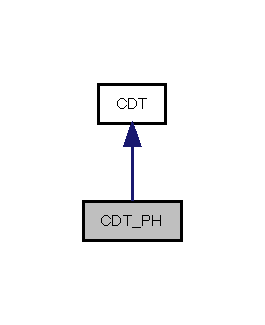
\includegraphics[width=127pt]{class_c_d_t___p_h__inherit__graph}
\end{center}
\end{figure}


Collaboration diagram for C\+D\+T\+\_\+\+PH\+:
\nopagebreak
\begin{figure}[H]
\begin{center}
\leavevmode
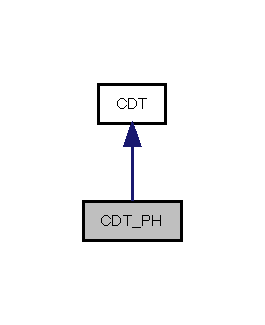
\includegraphics[width=127pt]{class_c_d_t___p_h__coll__graph}
\end{center}
\end{figure}
\subsection*{Public Member Functions}
\begin{DoxyCompactItemize}
\item 
\mbox{\hyperlink{class_c_d_t___p_h_a463a6fb9be715115dfc6b019d4788cbc}{C\+D\+T\+\_\+\+PH}} (double gamma, double lambda)
\begin{DoxyCompactList}\small\item\em Constructor of \mbox{\hyperlink{class_c_d_t___p_h}{C\+D\+T\+\_\+\+PH}}, i.\+e. a \mbox{\hyperlink{class_c_d_t}{C\+DT}} with the omnibus Page-\/\+Hinkley test. \end{DoxyCompactList}\item 
\mbox{\hyperlink{class_c_d_t___result}{C\+D\+T\+\_\+\+Result}} \mbox{\hyperlink{class_c_d_t___p_h_a58f56f0997012d0f350cc5721ef8a9e0}{run}} (double reward) override
\begin{DoxyCompactList}\small\item\em run the \mbox{\hyperlink{class_c_d_t___p_h}{C\+D\+T\+\_\+\+PH}} algorithm \end{DoxyCompactList}\item 
void \mbox{\hyperlink{class_c_d_t___p_h_adace7acacaeb66d3d2a292ccb69ac821}{reset}} () override
\begin{DoxyCompactList}\small\item\em reset the \mbox{\hyperlink{class_c_d_t___p_h}{C\+D\+T\+\_\+\+PH}} algorithm \end{DoxyCompactList}\end{DoxyCompactItemize}


\subsection{Detailed Description}
\mbox{\hyperlink{class_c_d_t}{C\+DT}} with the omnibus test Page-\/\+Hinkley. 

\subsection{Constructor \& Destructor Documentation}
\mbox{\Hypertarget{class_c_d_t___p_h_a463a6fb9be715115dfc6b019d4788cbc}\label{class_c_d_t___p_h_a463a6fb9be715115dfc6b019d4788cbc}} 
\index{C\+D\+T\+\_\+\+PH@{C\+D\+T\+\_\+\+PH}!C\+D\+T\+\_\+\+PH@{C\+D\+T\+\_\+\+PH}}
\index{C\+D\+T\+\_\+\+PH@{C\+D\+T\+\_\+\+PH}!C\+D\+T\+\_\+\+PH@{C\+D\+T\+\_\+\+PH}}
\subsubsection{\texorpdfstring{C\+D\+T\+\_\+\+P\+H()}{CDT\_PH()}}
{\footnotesize\ttfamily C\+D\+T\+\_\+\+P\+H\+::\+C\+D\+T\+\_\+\+PH (\begin{DoxyParamCaption}\item[{double}]{gamma,  }\item[{double}]{lambda }\end{DoxyParamCaption})}



Constructor of \mbox{\hyperlink{class_c_d_t___p_h}{C\+D\+T\+\_\+\+PH}}, i.\+e. a \mbox{\hyperlink{class_c_d_t}{C\+DT}} with the omnibus Page-\/\+Hinkley test. 


\begin{DoxyParams}{Parameters}
{\em gamma} & double, minimum expected mean variation \\
\hline
{\em lambda} & double, threshold for the PH statistic \\
\hline
\end{DoxyParams}


\subsection{Member Function Documentation}
\mbox{\Hypertarget{class_c_d_t___p_h_adace7acacaeb66d3d2a292ccb69ac821}\label{class_c_d_t___p_h_adace7acacaeb66d3d2a292ccb69ac821}} 
\index{C\+D\+T\+\_\+\+PH@{C\+D\+T\+\_\+\+PH}!reset@{reset}}
\index{reset@{reset}!C\+D\+T\+\_\+\+PH@{C\+D\+T\+\_\+\+PH}}
\subsubsection{\texorpdfstring{reset()}{reset()}}
{\footnotesize\ttfamily void C\+D\+T\+\_\+\+P\+H\+::reset (\begin{DoxyParamCaption}{ }\end{DoxyParamCaption})\hspace{0.3cm}{\ttfamily [override]}, {\ttfamily [virtual]}}



reset the \mbox{\hyperlink{class_c_d_t___p_h}{C\+D\+T\+\_\+\+PH}} algorithm 



Implements \mbox{\hyperlink{class_c_d_t_a46446ec219a819466ff418d9ab7aa728}{C\+DT}}.

\mbox{\Hypertarget{class_c_d_t___p_h_a58f56f0997012d0f350cc5721ef8a9e0}\label{class_c_d_t___p_h_a58f56f0997012d0f350cc5721ef8a9e0}} 
\index{C\+D\+T\+\_\+\+PH@{C\+D\+T\+\_\+\+PH}!run@{run}}
\index{run@{run}!C\+D\+T\+\_\+\+PH@{C\+D\+T\+\_\+\+PH}}
\subsubsection{\texorpdfstring{run()}{run()}}
{\footnotesize\ttfamily \mbox{\hyperlink{class_c_d_t___result}{C\+D\+T\+\_\+\+Result}} C\+D\+T\+\_\+\+P\+H\+::run (\begin{DoxyParamCaption}\item[{double}]{reward }\end{DoxyParamCaption})\hspace{0.3cm}{\ttfamily [override]}, {\ttfamily [virtual]}}



run the \mbox{\hyperlink{class_c_d_t___p_h}{C\+D\+T\+\_\+\+PH}} algorithm 


\begin{DoxyParams}{Parameters}
{\em reward} & double, the new datum that must be analysed by the \mbox{\hyperlink{class_c_d_t}{C\+DT}} \\
\hline
\end{DoxyParams}
\begin{DoxyReturn}{Returns}
a \mbox{\hyperlink{class_c_d_t___result}{C\+D\+T\+\_\+\+Result}} that contains the alarm and the estimated timestep change (this second part is not implemented!) 
\end{DoxyReturn}


Implements \mbox{\hyperlink{class_c_d_t_a2493aeb166403f448ec689d2f7b85dbc}{C\+DT}}.



The documentation for this class was generated from the following files\+:\begin{DoxyCompactItemize}
\item 
src/\mbox{\hyperlink{cdt_8h}{cdt.\+h}}\item 
src/\mbox{\hyperlink{cdt_8cpp}{cdt.\+cpp}}\end{DoxyCompactItemize}

\hypertarget{class_c_d_t___p_h___r_h_o}{}\section{C\+D\+T\+\_\+\+P\+H\+\_\+\+R\+HO Class Reference}
\label{class_c_d_t___p_h___r_h_o}\index{C\+D\+T\+\_\+\+P\+H\+\_\+\+R\+HO@{C\+D\+T\+\_\+\+P\+H\+\_\+\+R\+HO}}


\mbox{\hyperlink{class_c_d_t}{C\+DT}} with the discounted omnibus test Page-\/\+Hinkley.  




{\ttfamily \#include $<$cdt.\+h$>$}



Inheritance diagram for C\+D\+T\+\_\+\+P\+H\+\_\+\+R\+HO\+:
\nopagebreak
\begin{figure}[H]
\begin{center}
\leavevmode
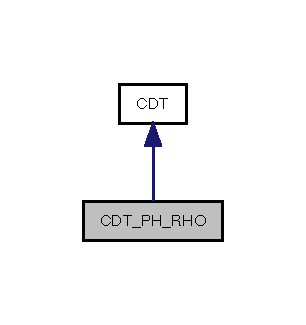
\includegraphics[width=147pt]{class_c_d_t___p_h___r_h_o__inherit__graph}
\end{center}
\end{figure}


Collaboration diagram for C\+D\+T\+\_\+\+P\+H\+\_\+\+R\+HO\+:
\nopagebreak
\begin{figure}[H]
\begin{center}
\leavevmode
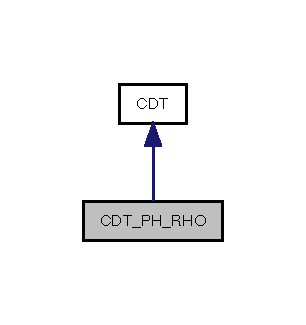
\includegraphics[width=147pt]{class_c_d_t___p_h___r_h_o__coll__graph}
\end{center}
\end{figure}
\subsection*{Public Member Functions}
\begin{DoxyCompactItemize}
\item 
\mbox{\hyperlink{class_c_d_t___p_h___r_h_o_ac9afe83ec08447b0d88c4e963fe95295}{C\+D\+T\+\_\+\+P\+H\+\_\+\+R\+HO}} (double gamma, double lambda, double rho)
\begin{DoxyCompactList}\small\item\em Constructor of \mbox{\hyperlink{class_c_d_t___p_h___r_h_o}{C\+D\+T\+\_\+\+P\+H\+\_\+\+R\+HO}}, i.\+e. a \mbox{\hyperlink{class_c_d_t}{C\+DT}} with the discounted omnibus Page-\/\+Hinkley test. \end{DoxyCompactList}\item 
\mbox{\hyperlink{class_c_d_t___result}{C\+D\+T\+\_\+\+Result}} \mbox{\hyperlink{class_c_d_t___p_h___r_h_o_a8c66d0d856204b5368e5b6cba989b0d7}{run}} (double reward) override
\begin{DoxyCompactList}\small\item\em run the \mbox{\hyperlink{class_c_d_t___p_h___r_h_o}{C\+D\+T\+\_\+\+P\+H\+\_\+\+R\+HO}} algorithm \end{DoxyCompactList}\item 
void \mbox{\hyperlink{class_c_d_t___p_h___r_h_o_acd4e4d53cbda5713ac60f07f002ec1c2}{reset}} () override
\begin{DoxyCompactList}\small\item\em reset the \mbox{\hyperlink{class_c_d_t___p_h___r_h_o}{C\+D\+T\+\_\+\+P\+H\+\_\+\+R\+HO}} algorithm \end{DoxyCompactList}\end{DoxyCompactItemize}


\subsection{Detailed Description}
\mbox{\hyperlink{class_c_d_t}{C\+DT}} with the discounted omnibus test Page-\/\+Hinkley. 

\subsection{Constructor \& Destructor Documentation}
\mbox{\Hypertarget{class_c_d_t___p_h___r_h_o_ac9afe83ec08447b0d88c4e963fe95295}\label{class_c_d_t___p_h___r_h_o_ac9afe83ec08447b0d88c4e963fe95295}} 
\index{C\+D\+T\+\_\+\+P\+H\+\_\+\+R\+HO@{C\+D\+T\+\_\+\+P\+H\+\_\+\+R\+HO}!C\+D\+T\+\_\+\+P\+H\+\_\+\+R\+HO@{C\+D\+T\+\_\+\+P\+H\+\_\+\+R\+HO}}
\index{C\+D\+T\+\_\+\+P\+H\+\_\+\+R\+HO@{C\+D\+T\+\_\+\+P\+H\+\_\+\+R\+HO}!C\+D\+T\+\_\+\+P\+H\+\_\+\+R\+HO@{C\+D\+T\+\_\+\+P\+H\+\_\+\+R\+HO}}
\subsubsection{\texorpdfstring{C\+D\+T\+\_\+\+P\+H\+\_\+\+R\+H\+O()}{CDT\_PH\_RHO()}}
{\footnotesize\ttfamily C\+D\+T\+\_\+\+P\+H\+\_\+\+R\+H\+O\+::\+C\+D\+T\+\_\+\+P\+H\+\_\+\+R\+HO (\begin{DoxyParamCaption}\item[{double}]{gamma,  }\item[{double}]{lambda,  }\item[{double}]{rho }\end{DoxyParamCaption})}



Constructor of \mbox{\hyperlink{class_c_d_t___p_h___r_h_o}{C\+D\+T\+\_\+\+P\+H\+\_\+\+R\+HO}}, i.\+e. a \mbox{\hyperlink{class_c_d_t}{C\+DT}} with the discounted omnibus Page-\/\+Hinkley test. 


\begin{DoxyParams}{Parameters}
{\em gamma} & double, minimum expected mean variation \\
\hline
{\em lambda} & double, threshold for the PH statistic \\
\hline
{\em rho} & double, discount factor \\
\hline
\end{DoxyParams}


\subsection{Member Function Documentation}
\mbox{\Hypertarget{class_c_d_t___p_h___r_h_o_acd4e4d53cbda5713ac60f07f002ec1c2}\label{class_c_d_t___p_h___r_h_o_acd4e4d53cbda5713ac60f07f002ec1c2}} 
\index{C\+D\+T\+\_\+\+P\+H\+\_\+\+R\+HO@{C\+D\+T\+\_\+\+P\+H\+\_\+\+R\+HO}!reset@{reset}}
\index{reset@{reset}!C\+D\+T\+\_\+\+P\+H\+\_\+\+R\+HO@{C\+D\+T\+\_\+\+P\+H\+\_\+\+R\+HO}}
\subsubsection{\texorpdfstring{reset()}{reset()}}
{\footnotesize\ttfamily void C\+D\+T\+\_\+\+P\+H\+\_\+\+R\+H\+O\+::reset (\begin{DoxyParamCaption}{ }\end{DoxyParamCaption})\hspace{0.3cm}{\ttfamily [override]}, {\ttfamily [virtual]}}



reset the \mbox{\hyperlink{class_c_d_t___p_h___r_h_o}{C\+D\+T\+\_\+\+P\+H\+\_\+\+R\+HO}} algorithm 



Implements \mbox{\hyperlink{class_c_d_t_a46446ec219a819466ff418d9ab7aa728}{C\+DT}}.

\mbox{\Hypertarget{class_c_d_t___p_h___r_h_o_a8c66d0d856204b5368e5b6cba989b0d7}\label{class_c_d_t___p_h___r_h_o_a8c66d0d856204b5368e5b6cba989b0d7}} 
\index{C\+D\+T\+\_\+\+P\+H\+\_\+\+R\+HO@{C\+D\+T\+\_\+\+P\+H\+\_\+\+R\+HO}!run@{run}}
\index{run@{run}!C\+D\+T\+\_\+\+P\+H\+\_\+\+R\+HO@{C\+D\+T\+\_\+\+P\+H\+\_\+\+R\+HO}}
\subsubsection{\texorpdfstring{run()}{run()}}
{\footnotesize\ttfamily \mbox{\hyperlink{class_c_d_t___result}{C\+D\+T\+\_\+\+Result}} C\+D\+T\+\_\+\+P\+H\+\_\+\+R\+H\+O\+::run (\begin{DoxyParamCaption}\item[{double}]{reward }\end{DoxyParamCaption})\hspace{0.3cm}{\ttfamily [override]}, {\ttfamily [virtual]}}



run the \mbox{\hyperlink{class_c_d_t___p_h___r_h_o}{C\+D\+T\+\_\+\+P\+H\+\_\+\+R\+HO}} algorithm 


\begin{DoxyParams}{Parameters}
{\em reward} & double, the new datum that must be analysed by the \mbox{\hyperlink{class_c_d_t}{C\+DT}} \\
\hline
\end{DoxyParams}
\begin{DoxyReturn}{Returns}
a \mbox{\hyperlink{class_c_d_t___result}{C\+D\+T\+\_\+\+Result}} that contains the alarm and the estimated timestep change (this second part is not implemented!) 
\end{DoxyReturn}


Implements \mbox{\hyperlink{class_c_d_t_a2493aeb166403f448ec689d2f7b85dbc}{C\+DT}}.



The documentation for this class was generated from the following files\+:\begin{DoxyCompactItemize}
\item 
src/\mbox{\hyperlink{cdt_8h}{cdt.\+h}}\item 
src/\mbox{\hyperlink{cdt_8cpp}{cdt.\+cpp}}\end{DoxyCompactItemize}

\hypertarget{class_c_d_t___result}{}\section{C\+D\+T\+\_\+\+Result Class Reference}
\label{class_c_d_t___result}\index{C\+D\+T\+\_\+\+Result@{C\+D\+T\+\_\+\+Result}}


Class that contains the result of a call to a generic \mbox{\hyperlink{class_c_d_t}{C\+DT}} procedure. It contains two things\+: a boolean alarm that represents whether or not a change has been detected; an integer that is the estimate of the timestep of the change.  




{\ttfamily \#include $<$cdt.\+h$>$}

\subsection*{Public Member Functions}
\begin{DoxyCompactItemize}
\item 
\mbox{\hyperlink{class_c_d_t___result_a55f9f8ce1a3f02a77502e34788abefb8}{C\+D\+T\+\_\+\+Result}} (bool \mbox{\hyperlink{class_c_d_t___result_a4e9efc182d7b730a00f5b14d8e9a94d7}{alarm}}, int \mbox{\hyperlink{class_c_d_t___result_a69cea3ae579857edc859347aa47f41b6}{change\+\_\+estimate}})
\begin{DoxyCompactList}\small\item\em Constructor of C\+D\+T\+\_\+result. \end{DoxyCompactList}\end{DoxyCompactItemize}
\subsection*{Public Attributes}
\begin{DoxyCompactItemize}
\item 
bool \mbox{\hyperlink{class_c_d_t___result_a4e9efc182d7b730a00f5b14d8e9a94d7}{alarm}}
\item 
int \mbox{\hyperlink{class_c_d_t___result_a69cea3ae579857edc859347aa47f41b6}{change\+\_\+estimate}}
\end{DoxyCompactItemize}


\subsection{Detailed Description}
Class that contains the result of a call to a generic \mbox{\hyperlink{class_c_d_t}{C\+DT}} procedure. It contains two things\+: a boolean alarm that represents whether or not a change has been detected; an integer that is the estimate of the timestep of the change. 

\subsection{Constructor \& Destructor Documentation}
\mbox{\Hypertarget{class_c_d_t___result_a55f9f8ce1a3f02a77502e34788abefb8}\label{class_c_d_t___result_a55f9f8ce1a3f02a77502e34788abefb8}} 
\index{C\+D\+T\+\_\+\+Result@{C\+D\+T\+\_\+\+Result}!C\+D\+T\+\_\+\+Result@{C\+D\+T\+\_\+\+Result}}
\index{C\+D\+T\+\_\+\+Result@{C\+D\+T\+\_\+\+Result}!C\+D\+T\+\_\+\+Result@{C\+D\+T\+\_\+\+Result}}
\subsubsection{\texorpdfstring{C\+D\+T\+\_\+\+Result()}{CDT\_Result()}}
{\footnotesize\ttfamily C\+D\+T\+\_\+\+Result\+::\+C\+D\+T\+\_\+\+Result (\begin{DoxyParamCaption}\item[{bool}]{alarm,  }\item[{int}]{change\+\_\+estimate }\end{DoxyParamCaption})}



Constructor of C\+D\+T\+\_\+result. 


\begin{DoxyParams}{Parameters}
{\em alarm} & boolean, represents whether a change has been detected or not \\
\hline
{\em change\+\_\+estimate} & integer, represents the estimated timestep of the change \\
\hline
\end{DoxyParams}


\subsection{Member Data Documentation}
\mbox{\Hypertarget{class_c_d_t___result_a4e9efc182d7b730a00f5b14d8e9a94d7}\label{class_c_d_t___result_a4e9efc182d7b730a00f5b14d8e9a94d7}} 
\index{C\+D\+T\+\_\+\+Result@{C\+D\+T\+\_\+\+Result}!alarm@{alarm}}
\index{alarm@{alarm}!C\+D\+T\+\_\+\+Result@{C\+D\+T\+\_\+\+Result}}
\subsubsection{\texorpdfstring{alarm}{alarm}}
{\footnotesize\ttfamily bool C\+D\+T\+\_\+\+Result\+::alarm}

\mbox{\Hypertarget{class_c_d_t___result_a69cea3ae579857edc859347aa47f41b6}\label{class_c_d_t___result_a69cea3ae579857edc859347aa47f41b6}} 
\index{C\+D\+T\+\_\+\+Result@{C\+D\+T\+\_\+\+Result}!change\+\_\+estimate@{change\+\_\+estimate}}
\index{change\+\_\+estimate@{change\+\_\+estimate}!C\+D\+T\+\_\+\+Result@{C\+D\+T\+\_\+\+Result}}
\subsubsection{\texorpdfstring{change\+\_\+estimate}{change\_estimate}}
{\footnotesize\ttfamily int C\+D\+T\+\_\+\+Result\+::change\+\_\+estimate}



The documentation for this class was generated from the following files\+:\begin{DoxyCompactItemize}
\item 
src/\mbox{\hyperlink{cdt_8h}{cdt.\+h}}\item 
src/\mbox{\hyperlink{cdt_8cpp}{cdt.\+cpp}}\end{DoxyCompactItemize}

\hypertarget{class_d___u_c_b}{}\section{D\+\_\+\+U\+CB Class Reference}
\label{class_d___u_c_b}\index{D\+\_\+\+U\+CB@{D\+\_\+\+U\+CB}}


discounted \mbox{\hyperlink{class_u_c_b}{U\+CB}} algorithm  




{\ttfamily \#include $<$ucb.\+h$>$}



Inheritance diagram for D\+\_\+\+U\+CB\+:
\nopagebreak
\begin{figure}[H]
\begin{center}
\leavevmode
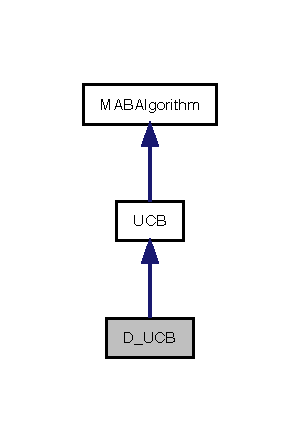
\includegraphics[width=144pt]{class_d___u_c_b__inherit__graph}
\end{center}
\end{figure}


Collaboration diagram for D\+\_\+\+U\+CB\+:
\nopagebreak
\begin{figure}[H]
\begin{center}
\leavevmode
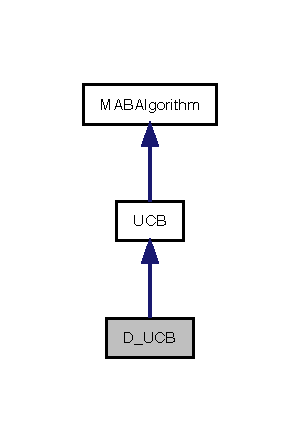
\includegraphics[width=144pt]{class_d___u_c_b__coll__graph}
\end{center}
\end{figure}
\subsection*{Public Member Functions}
\begin{DoxyCompactItemize}
\item 
\mbox{\hyperlink{class_d___u_c_b_adc6258dbbe7449d0ec6b7b7bb3ae88e8}{D\+\_\+\+U\+CB}} (string \mbox{\hyperlink{class_m_a_b_algorithm_a77b10ecc4b49d519c557f65358167b82}{name}}, int \mbox{\hyperlink{class_m_a_b_algorithm_a340fa9e83e85b092f2c6125fc4e8549b}{num\+\_\+of\+\_\+arms}}, double gamma, double B, double epsilon)
\item 
int \mbox{\hyperlink{class_d___u_c_b_ac48b99c21eb02361707988f6ac012408}{choose\+\_\+action}} () override
\item 
void \mbox{\hyperlink{class_d___u_c_b_a23b79f3f23095ae6e824b36a3856ff7c}{receive\+\_\+reward}} (double reward, int pulled\+\_\+arm) override
\begin{DoxyCompactList}\small\item\em Update the internal variables of the algorithm according to the new received reward. \end{DoxyCompactList}\item 
void \mbox{\hyperlink{class_d___u_c_b_a454ffcd1e17989f0b049790cfc5fc515}{reset}} (int action=-\/1) override
\begin{DoxyCompactList}\small\item\em resets the internal variables of the algorithm \end{DoxyCompactList}\end{DoxyCompactItemize}
\subsection*{Additional Inherited Members}


\subsection{Detailed Description}
discounted \mbox{\hyperlink{class_u_c_b}{U\+CB}} algorithm 

\subsection{Constructor \& Destructor Documentation}
\mbox{\Hypertarget{class_d___u_c_b_adc6258dbbe7449d0ec6b7b7bb3ae88e8}\label{class_d___u_c_b_adc6258dbbe7449d0ec6b7b7bb3ae88e8}} 
\index{D\+\_\+\+U\+CB@{D\+\_\+\+U\+CB}!D\+\_\+\+U\+CB@{D\+\_\+\+U\+CB}}
\index{D\+\_\+\+U\+CB@{D\+\_\+\+U\+CB}!D\+\_\+\+U\+CB@{D\+\_\+\+U\+CB}}
\subsubsection{\texorpdfstring{D\+\_\+\+U\+C\+B()}{D\_UCB()}}
{\footnotesize\ttfamily D\+\_\+\+U\+C\+B\+::\+D\+\_\+\+U\+CB (\begin{DoxyParamCaption}\item[{string}]{name,  }\item[{int}]{num\+\_\+of\+\_\+arms,  }\item[{double}]{gamma,  }\item[{double}]{B,  }\item[{double}]{epsilon }\end{DoxyParamCaption})}


\begin{DoxyParams}{Parameters}
{\em name} & string, id of the algorithm \\
\hline
{\em num\+\_\+of\+\_\+arms} & integer, number of arms the algorithm will work on \\
\hline
{\em gamma} & double in (0,1), discount factor \\
\hline
{\em B} & double, confidence parameter \\
\hline
{\em epsilon} & double in (1,inf), confidence parameter \\
\hline
\end{DoxyParams}


\subsection{Member Function Documentation}
\mbox{\Hypertarget{class_d___u_c_b_ac48b99c21eb02361707988f6ac012408}\label{class_d___u_c_b_ac48b99c21eb02361707988f6ac012408}} 
\index{D\+\_\+\+U\+CB@{D\+\_\+\+U\+CB}!choose\+\_\+action@{choose\+\_\+action}}
\index{choose\+\_\+action@{choose\+\_\+action}!D\+\_\+\+U\+CB@{D\+\_\+\+U\+CB}}
\subsubsection{\texorpdfstring{choose\+\_\+action()}{choose\_action()}}
{\footnotesize\ttfamily int D\+\_\+\+U\+C\+B\+::choose\+\_\+action (\begin{DoxyParamCaption}{ }\end{DoxyParamCaption})\hspace{0.3cm}{\ttfamily [override]}, {\ttfamily [virtual]}}

\begin{DoxyReturn}{Returns}
an integer representing the chosen arm 
\end{DoxyReturn}


Implements \mbox{\hyperlink{class_m_a_b_algorithm_afb48f01df0e1860d19759f6e20335007}{M\+A\+B\+Algorithm}}.

\mbox{\Hypertarget{class_d___u_c_b_a23b79f3f23095ae6e824b36a3856ff7c}\label{class_d___u_c_b_a23b79f3f23095ae6e824b36a3856ff7c}} 
\index{D\+\_\+\+U\+CB@{D\+\_\+\+U\+CB}!receive\+\_\+reward@{receive\+\_\+reward}}
\index{receive\+\_\+reward@{receive\+\_\+reward}!D\+\_\+\+U\+CB@{D\+\_\+\+U\+CB}}
\subsubsection{\texorpdfstring{receive\+\_\+reward()}{receive\_reward()}}
{\footnotesize\ttfamily void D\+\_\+\+U\+C\+B\+::receive\+\_\+reward (\begin{DoxyParamCaption}\item[{double}]{reward,  }\item[{int}]{pulled\+\_\+arm }\end{DoxyParamCaption})\hspace{0.3cm}{\ttfamily [override]}, {\ttfamily [virtual]}}



Update the internal variables of the algorithm according to the new received reward. 


\begin{DoxyParams}{Parameters}
{\em reward} & double, new received reward \\
\hline
{\em pulled\+\_\+arm} & integer, represents the pulled arm \\
\hline
\end{DoxyParams}


Reimplemented from \mbox{\hyperlink{class_m_a_b_algorithm_aa584b3d6b86fa050e3389be9781b5782}{M\+A\+B\+Algorithm}}.

\mbox{\Hypertarget{class_d___u_c_b_a454ffcd1e17989f0b049790cfc5fc515}\label{class_d___u_c_b_a454ffcd1e17989f0b049790cfc5fc515}} 
\index{D\+\_\+\+U\+CB@{D\+\_\+\+U\+CB}!reset@{reset}}
\index{reset@{reset}!D\+\_\+\+U\+CB@{D\+\_\+\+U\+CB}}
\subsubsection{\texorpdfstring{reset()}{reset()}}
{\footnotesize\ttfamily void D\+\_\+\+U\+C\+B\+::reset (\begin{DoxyParamCaption}\item[{int}]{action = {\ttfamily -\/1} }\end{DoxyParamCaption})\hspace{0.3cm}{\ttfamily [override]}, {\ttfamily [virtual]}}



resets the internal variables of the algorithm 


\begin{DoxyParams}{Parameters}
{\em action} & integer, specifies which variables to reset. If in (0, num\+\_\+of\+\_\+arms -\/ 1), then it resets only the info related to such arm. If == -\/1, resets all the arms. \\
\hline
\end{DoxyParams}


Reimplemented from \mbox{\hyperlink{class_m_a_b_algorithm_ad5761cee0b0e3421d1f043dbcc0b5f85}{M\+A\+B\+Algorithm}}.



The documentation for this class was generated from the following files\+:\begin{DoxyCompactItemize}
\item 
src/\mbox{\hyperlink{ucb_8h}{ucb.\+h}}\item 
src/\mbox{\hyperlink{ucb_8cpp}{ucb.\+cpp}}\end{DoxyCompactItemize}

\hypertarget{class_distribution}{}\section{Distribution Class Reference}
\label{class_distribution}\index{Distribution@{Distribution}}


Base class of all the \mbox{\hyperlink{class_distribution}{Distribution}} classes.  




{\ttfamily \#include $<$distribution.\+h$>$}



Inheritance diagram for Distribution\+:
\nopagebreak
\begin{figure}[H]
\begin{center}
\leavevmode
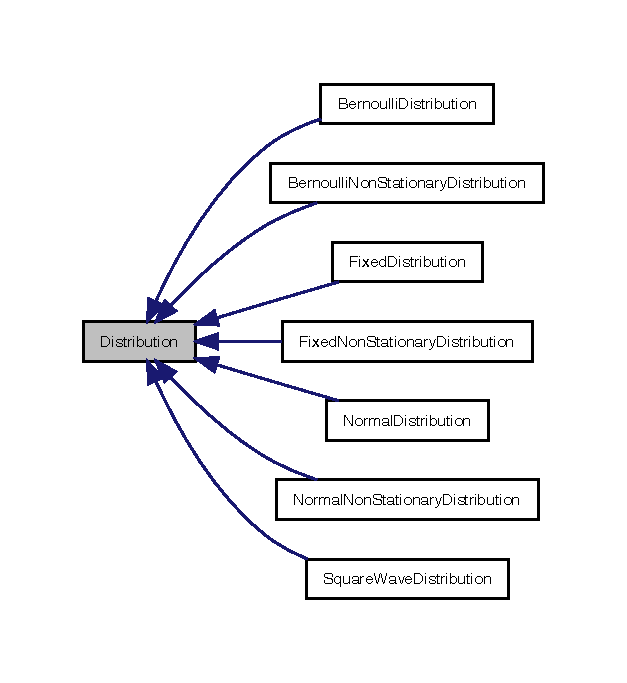
\includegraphics[width=301pt]{class_distribution__inherit__graph}
\end{center}
\end{figure}
\subsection*{Public Member Functions}
\begin{DoxyCompactItemize}
\item 
\mbox{\hyperlink{class_distribution_a7734801d8703a4d0f43a83d7439e5ca6}{Distribution}} (string \mbox{\hyperlink{class_distribution_ab3b7be02f0401cb76beb2e744b6161f9}{name}})
\begin{DoxyCompactList}\small\item\em Constructor of \mbox{\hyperlink{class_distribution}{Distribution}}. \end{DoxyCompactList}\item 
\mbox{\hyperlink{class_distribution_a405bc928b7710b5362c7070489a7362e}{Distribution}} (string \mbox{\hyperlink{class_distribution_ab3b7be02f0401cb76beb2e744b6161f9}{name}}, boost\+::mt19937 \&\mbox{\hyperlink{class_distribution_ac8915a45ce85ab6b7506fa42bb850a89}{rng}})
\begin{DoxyCompactList}\small\item\em Constructor of \mbox{\hyperlink{class_distribution}{Distribution}}. \end{DoxyCompactList}\item 
virtual double \mbox{\hyperlink{class_distribution_a742b398af4a461243028cce3c47d8080}{draw}} (int timestep)=0
\begin{DoxyCompactList}\small\item\em draw the reward for a certain timestep \end{DoxyCompactList}\item 
virtual string \mbox{\hyperlink{class_distribution_ac41d57a4d7f82041810f886590a236a5}{to\+File}} ()=0
\begin{DoxyCompactList}\small\item\em build a representation of this \mbox{\hyperlink{class_distribution}{Distribution}} so that it can be printed to a file and be later analysed by another script \end{DoxyCompactList}\item 
virtual double \mbox{\hyperlink{class_distribution_ac9c74d18549f532caa09ae86d8b25b55}{get\+\_\+mean}} (int timestep)=0
\end{DoxyCompactItemize}
\subsection*{Public Attributes}
\begin{DoxyCompactItemize}
\item 
string \mbox{\hyperlink{class_distribution_ab3b7be02f0401cb76beb2e744b6161f9}{name}}
\item 
bool \mbox{\hyperlink{class_distribution_a58fa80cadc13b26e12e9ed34aa8b926c}{is\+\_\+mab}}
\end{DoxyCompactItemize}
\subsection*{Protected Attributes}
\begin{DoxyCompactItemize}
\item 
boost\+::mt19937 $\ast$ \mbox{\hyperlink{class_distribution_ac8915a45ce85ab6b7506fa42bb850a89}{rng}}
\end{DoxyCompactItemize}


\subsection{Detailed Description}
Base class of all the \mbox{\hyperlink{class_distribution}{Distribution}} classes. 


\begin{DoxyParams}{Parameters}
{\em name} & string, id of the distribution \\
\hline
\end{DoxyParams}


\subsection{Constructor \& Destructor Documentation}
\mbox{\Hypertarget{class_distribution_a7734801d8703a4d0f43a83d7439e5ca6}\label{class_distribution_a7734801d8703a4d0f43a83d7439e5ca6}} 
\index{Distribution@{Distribution}!Distribution@{Distribution}}
\index{Distribution@{Distribution}!Distribution@{Distribution}}
\subsubsection{\texorpdfstring{Distribution()}{Distribution()}\hspace{0.1cm}{\footnotesize\ttfamily [1/2]}}
{\footnotesize\ttfamily Distribution\+::\+Distribution (\begin{DoxyParamCaption}\item[{string}]{name }\end{DoxyParamCaption})}



Constructor of \mbox{\hyperlink{class_distribution}{Distribution}}. 


\begin{DoxyParams}{Parameters}
{\em name} & string, id of the distribution \\
\hline
\end{DoxyParams}
\mbox{\Hypertarget{class_distribution_a405bc928b7710b5362c7070489a7362e}\label{class_distribution_a405bc928b7710b5362c7070489a7362e}} 
\index{Distribution@{Distribution}!Distribution@{Distribution}}
\index{Distribution@{Distribution}!Distribution@{Distribution}}
\subsubsection{\texorpdfstring{Distribution()}{Distribution()}\hspace{0.1cm}{\footnotesize\ttfamily [2/2]}}
{\footnotesize\ttfamily Distribution\+::\+Distribution (\begin{DoxyParamCaption}\item[{string}]{name,  }\item[{boost\+::mt19937 \&}]{rng }\end{DoxyParamCaption})}



Constructor of \mbox{\hyperlink{class_distribution}{Distribution}}. 


\begin{DoxyParams}{Parameters}
{\em name} & string, id of the distribution \\
\hline
{\em rng} & boost\+::mt19937\&, rng used to generate data \\
\hline
\end{DoxyParams}


\subsection{Member Function Documentation}
\mbox{\Hypertarget{class_distribution_a742b398af4a461243028cce3c47d8080}\label{class_distribution_a742b398af4a461243028cce3c47d8080}} 
\index{Distribution@{Distribution}!draw@{draw}}
\index{draw@{draw}!Distribution@{Distribution}}
\subsubsection{\texorpdfstring{draw()}{draw()}}
{\footnotesize\ttfamily virtual double Distribution\+::draw (\begin{DoxyParamCaption}\item[{int}]{timestep }\end{DoxyParamCaption})\hspace{0.3cm}{\ttfamily [pure virtual]}}



draw the reward for a certain timestep 


\begin{DoxyParams}{Parameters}
{\em timestep} & int, timestep at which the reward is drawn \\
\hline
\end{DoxyParams}
\begin{DoxyReturn}{Returns}
a double which is the drawn reward 
\end{DoxyReturn}


Implemented in \mbox{\hyperlink{class_square_wave_distribution_a7994182585346203ec158272cc39b17e}{Square\+Wave\+Distribution}}, \mbox{\hyperlink{class_bernoulli_non_stationary_distribution_a4aee952b4eebc5d36ff318b4c30f4a5d}{Bernoulli\+Non\+Stationary\+Distribution}}, \mbox{\hyperlink{class_bernoulli_distribution_ae733579a1c78c01ba8d915bfb8d7b088}{Bernoulli\+Distribution}}, \mbox{\hyperlink{class_fixed_non_stationary_distribution_afd4a118bfe398f700e93430ca05dbae6}{Fixed\+Non\+Stationary\+Distribution}}, \mbox{\hyperlink{class_fixed_distribution_a1babd43b5bbc4e0a720ca77690c9adad}{Fixed\+Distribution}}, \mbox{\hyperlink{class_normal_non_stationary_distribution_a0bd7d418784487c822c330f2b51a6112}{Normal\+Non\+Stationary\+Distribution}}, and \mbox{\hyperlink{class_normal_distribution_abd089ca83f0b358099aba4873a86f091}{Normal\+Distribution}}.

\mbox{\Hypertarget{class_distribution_ac9c74d18549f532caa09ae86d8b25b55}\label{class_distribution_ac9c74d18549f532caa09ae86d8b25b55}} 
\index{Distribution@{Distribution}!get\+\_\+mean@{get\+\_\+mean}}
\index{get\+\_\+mean@{get\+\_\+mean}!Distribution@{Distribution}}
\subsubsection{\texorpdfstring{get\+\_\+mean()}{get\_mean()}}
{\footnotesize\ttfamily virtual double Distribution\+::get\+\_\+mean (\begin{DoxyParamCaption}\item[{int}]{timestep }\end{DoxyParamCaption})\hspace{0.3cm}{\ttfamily [pure virtual]}}


\begin{DoxyParams}{Parameters}
{\em timestep} & integer, the timestep at which the mean is asked \\
\hline
\end{DoxyParams}
\begin{DoxyReturn}{Returns}
the mean (double) at the specified timestep 
\end{DoxyReturn}


Implemented in \mbox{\hyperlink{class_square_wave_distribution_ac2e790a852c02473e70e4ff5090cfc51}{Square\+Wave\+Distribution}}, \mbox{\hyperlink{class_bernoulli_non_stationary_distribution_ab1cf34057259a933b7957fbff28ed442}{Bernoulli\+Non\+Stationary\+Distribution}}, \mbox{\hyperlink{class_bernoulli_distribution_a7756a9b4861bf90bc7cc346e77b40603}{Bernoulli\+Distribution}}, \mbox{\hyperlink{class_fixed_non_stationary_distribution_aa9ed51fbf731f288a76a3a9e0aee8390}{Fixed\+Non\+Stationary\+Distribution}}, \mbox{\hyperlink{class_fixed_distribution_af9199f9076551694af2397c7dd69096e}{Fixed\+Distribution}}, \mbox{\hyperlink{class_normal_non_stationary_distribution_ae3d2f4fb0e5c9b706c84d05ac14de2aa}{Normal\+Non\+Stationary\+Distribution}}, and \mbox{\hyperlink{class_normal_distribution_ad3165276bf35135409974e73f3cdd6d0}{Normal\+Distribution}}.

\mbox{\Hypertarget{class_distribution_ac41d57a4d7f82041810f886590a236a5}\label{class_distribution_ac41d57a4d7f82041810f886590a236a5}} 
\index{Distribution@{Distribution}!to\+File@{to\+File}}
\index{to\+File@{to\+File}!Distribution@{Distribution}}
\subsubsection{\texorpdfstring{to\+File()}{toFile()}}
{\footnotesize\ttfamily virtual string Distribution\+::to\+File (\begin{DoxyParamCaption}{ }\end{DoxyParamCaption})\hspace{0.3cm}{\ttfamily [pure virtual]}}



build a representation of this \mbox{\hyperlink{class_distribution}{Distribution}} so that it can be printed to a file and be later analysed by another script 

\begin{DoxyReturn}{Returns}
a string that represents this \mbox{\hyperlink{class_distribution}{Distribution}} 
\end{DoxyReturn}


Implemented in \mbox{\hyperlink{class_square_wave_distribution_a8ba3fbbf02f23f02697f34f841e9a870}{Square\+Wave\+Distribution}}, \mbox{\hyperlink{class_bernoulli_non_stationary_distribution_a5db3f4675ff988f3c775a939f8ef4847}{Bernoulli\+Non\+Stationary\+Distribution}}, \mbox{\hyperlink{class_bernoulli_distribution_a29f9f1014234828255def7bf9872b086}{Bernoulli\+Distribution}}, \mbox{\hyperlink{class_fixed_non_stationary_distribution_aaea49214758451b31f83a272af1626e0}{Fixed\+Non\+Stationary\+Distribution}}, \mbox{\hyperlink{class_fixed_distribution_a6396ce831e3ff31ecc39bda45e3ecb08}{Fixed\+Distribution}}, \mbox{\hyperlink{class_normal_non_stationary_distribution_a4f2f7cdfacf8b54a0cb2b5237213a693}{Normal\+Non\+Stationary\+Distribution}}, and \mbox{\hyperlink{class_normal_distribution_aba8376a8b209a82d8d042c9d2a4c412c}{Normal\+Distribution}}.



\subsection{Member Data Documentation}
\mbox{\Hypertarget{class_distribution_a58fa80cadc13b26e12e9ed34aa8b926c}\label{class_distribution_a58fa80cadc13b26e12e9ed34aa8b926c}} 
\index{Distribution@{Distribution}!is\+\_\+mab@{is\+\_\+mab}}
\index{is\+\_\+mab@{is\+\_\+mab}!Distribution@{Distribution}}
\subsubsection{\texorpdfstring{is\+\_\+mab}{is\_mab}}
{\footnotesize\ttfamily bool Distribution\+::is\+\_\+mab}

\mbox{\Hypertarget{class_distribution_ab3b7be02f0401cb76beb2e744b6161f9}\label{class_distribution_ab3b7be02f0401cb76beb2e744b6161f9}} 
\index{Distribution@{Distribution}!name@{name}}
\index{name@{name}!Distribution@{Distribution}}
\subsubsection{\texorpdfstring{name}{name}}
{\footnotesize\ttfamily string Distribution\+::name}

\mbox{\Hypertarget{class_distribution_ac8915a45ce85ab6b7506fa42bb850a89}\label{class_distribution_ac8915a45ce85ab6b7506fa42bb850a89}} 
\index{Distribution@{Distribution}!rng@{rng}}
\index{rng@{rng}!Distribution@{Distribution}}
\subsubsection{\texorpdfstring{rng}{rng}}
{\footnotesize\ttfamily boost\+::mt19937$\ast$ Distribution\+::rng\hspace{0.3cm}{\ttfamily [protected]}}



The documentation for this class was generated from the following files\+:\begin{DoxyCompactItemize}
\item 
src/\mbox{\hyperlink{distribution_8h}{distribution.\+h}}\item 
src/\mbox{\hyperlink{distribution_8cpp}{distribution.\+cpp}}\end{DoxyCompactItemize}

\hypertarget{class_e_x_p}{}\section{E\+XP Class Reference}
\label{class_e_x_p}\index{E\+XP@{E\+XP}}


base class of the \mbox{\hyperlink{class_e_x_p}{E\+XP}} algorithms  




{\ttfamily \#include $<$exp.\+h$>$}



Inheritance diagram for E\+XP\+:
\nopagebreak
\begin{figure}[H]
\begin{center}
\leavevmode
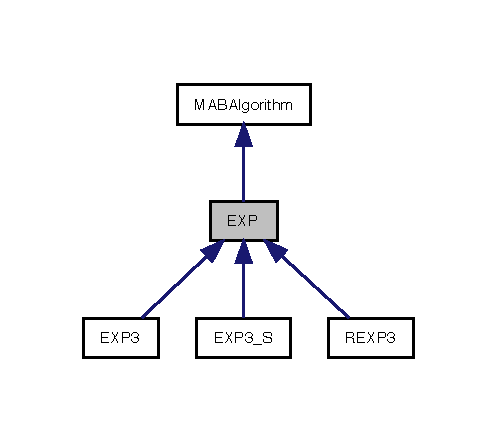
\includegraphics[width=239pt]{class_e_x_p__inherit__graph}
\end{center}
\end{figure}


Collaboration diagram for E\+XP\+:
\nopagebreak
\begin{figure}[H]
\begin{center}
\leavevmode
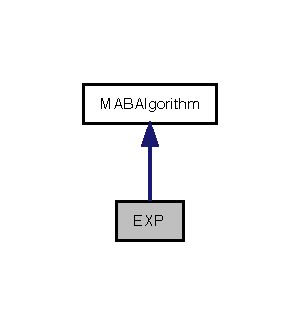
\includegraphics[width=144pt]{class_e_x_p__coll__graph}
\end{center}
\end{figure}
\subsection*{Public Member Functions}
\begin{DoxyCompactItemize}
\item 
\mbox{\hyperlink{class_e_x_p_a1ec218c13f58399e79bdca89f761c511}{E\+XP}} (string \mbox{\hyperlink{class_m_a_b_algorithm_a77b10ecc4b49d519c557f65358167b82}{name}}, int \mbox{\hyperlink{class_m_a_b_algorithm_a340fa9e83e85b092f2c6125fc4e8549b}{num\+\_\+of\+\_\+arms}})
\end{DoxyCompactItemize}
\subsection*{Additional Inherited Members}


\subsection{Detailed Description}
base class of the \mbox{\hyperlink{class_e_x_p}{E\+XP}} algorithms 

\subsection{Constructor \& Destructor Documentation}
\mbox{\Hypertarget{class_e_x_p_a1ec218c13f58399e79bdca89f761c511}\label{class_e_x_p_a1ec218c13f58399e79bdca89f761c511}} 
\index{E\+XP@{E\+XP}!E\+XP@{E\+XP}}
\index{E\+XP@{E\+XP}!E\+XP@{E\+XP}}
\subsubsection{\texorpdfstring{E\+X\+P()}{EXP()}}
{\footnotesize\ttfamily E\+X\+P\+::\+E\+XP (\begin{DoxyParamCaption}\item[{string}]{name,  }\item[{int}]{num\+\_\+of\+\_\+arms }\end{DoxyParamCaption})}


\begin{DoxyParams}{Parameters}
{\em name} & string, id of the algorithm \\
\hline
{\em num\+\_\+of\+\_\+arms} & integer, number of arms the algorithm will work on \\
\hline
\end{DoxyParams}


The documentation for this class was generated from the following files\+:\begin{DoxyCompactItemize}
\item 
src/\mbox{\hyperlink{exp_8h}{exp.\+h}}\item 
src/\mbox{\hyperlink{exp_8cpp}{exp.\+cpp}}\end{DoxyCompactItemize}

\hypertarget{class_e_x_p3}{}\section{E\+X\+P3 Class Reference}
\label{class_e_x_p3}\index{E\+X\+P3@{E\+X\+P3}}


\mbox{\hyperlink{class_e_x_p3}{E\+X\+P3}} algorithm.  




{\ttfamily \#include $<$exp.\+h$>$}



Inheritance diagram for E\+X\+P3\+:
\nopagebreak
\begin{figure}[H]
\begin{center}
\leavevmode
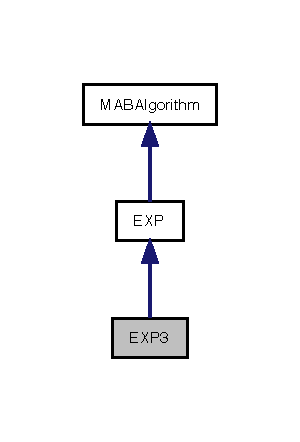
\includegraphics[width=144pt]{class_e_x_p3__inherit__graph}
\end{center}
\end{figure}


Collaboration diagram for E\+X\+P3\+:
\nopagebreak
\begin{figure}[H]
\begin{center}
\leavevmode
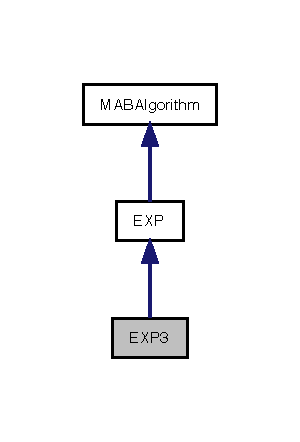
\includegraphics[width=144pt]{class_e_x_p3__coll__graph}
\end{center}
\end{figure}
\subsection*{Public Member Functions}
\begin{DoxyCompactItemize}
\item 
\mbox{\hyperlink{class_e_x_p3_adb52da022d3f30abb0784cfd63104231}{E\+X\+P3}} (string \mbox{\hyperlink{class_m_a_b_algorithm_a77b10ecc4b49d519c557f65358167b82}{name}}, int \mbox{\hyperlink{class_m_a_b_algorithm_a340fa9e83e85b092f2c6125fc4e8549b}{num\+\_\+of\+\_\+arms}}, double beta, double nu)
\begin{DoxyCompactList}\small\item\em constructor of \mbox{\hyperlink{class_e_x_p3}{E\+X\+P3}} \end{DoxyCompactList}\item 
int \mbox{\hyperlink{class_e_x_p3_adb52fc51fbc5ef97e3d67c2437634be8}{choose\+\_\+action}} () override
\item 
void \mbox{\hyperlink{class_e_x_p3_a9408f963aa533ffb298deba2fbc65529}{receive\+\_\+reward}} (double reward, int pulled\+\_\+arm) override
\begin{DoxyCompactList}\small\item\em Update the internal variables of the algorithm according to the new received reward. \end{DoxyCompactList}\item 
void \mbox{\hyperlink{class_e_x_p3_a30530aa50cd991eda2f9f2f170b92d0e}{reset}} (int action=-\/1) override
\begin{DoxyCompactList}\small\item\em resets the internal variables of the algorithm \end{DoxyCompactList}\end{DoxyCompactItemize}
\subsection*{Additional Inherited Members}


\subsection{Detailed Description}
\mbox{\hyperlink{class_e_x_p3}{E\+X\+P3}} algorithm. 

\subsection{Constructor \& Destructor Documentation}
\mbox{\Hypertarget{class_e_x_p3_adb52da022d3f30abb0784cfd63104231}\label{class_e_x_p3_adb52da022d3f30abb0784cfd63104231}} 
\index{E\+X\+P3@{E\+X\+P3}!E\+X\+P3@{E\+X\+P3}}
\index{E\+X\+P3@{E\+X\+P3}!E\+X\+P3@{E\+X\+P3}}
\subsubsection{\texorpdfstring{E\+X\+P3()}{EXP3()}}
{\footnotesize\ttfamily E\+X\+P3\+::\+E\+X\+P3 (\begin{DoxyParamCaption}\item[{string}]{name,  }\item[{int}]{num\+\_\+of\+\_\+arms,  }\item[{double}]{beta,  }\item[{double}]{nu }\end{DoxyParamCaption})}



constructor of \mbox{\hyperlink{class_e_x_p3}{E\+X\+P3}} 


\begin{DoxyParams}{Parameters}
{\em name} & string, id of the algorithm \\
\hline
{\em num\+\_\+of\+\_\+arms} & integer, number of arms the algorithm will work on \\
\hline
{\em beta} & double, exploration parameter (between 0 and 1) \\
\hline
{\em nu} & double, exponential update parameter \\
\hline
\end{DoxyParams}


\subsection{Member Function Documentation}
\mbox{\Hypertarget{class_e_x_p3_adb52fc51fbc5ef97e3d67c2437634be8}\label{class_e_x_p3_adb52fc51fbc5ef97e3d67c2437634be8}} 
\index{E\+X\+P3@{E\+X\+P3}!choose\+\_\+action@{choose\+\_\+action}}
\index{choose\+\_\+action@{choose\+\_\+action}!E\+X\+P3@{E\+X\+P3}}
\subsubsection{\texorpdfstring{choose\+\_\+action()}{choose\_action()}}
{\footnotesize\ttfamily int E\+X\+P3\+::choose\+\_\+action (\begin{DoxyParamCaption}{ }\end{DoxyParamCaption})\hspace{0.3cm}{\ttfamily [override]}, {\ttfamily [virtual]}}

\begin{DoxyReturn}{Returns}
an integer representing the chosen arm 
\end{DoxyReturn}


Implements \mbox{\hyperlink{class_m_a_b_algorithm_afb48f01df0e1860d19759f6e20335007}{M\+A\+B\+Algorithm}}.

\mbox{\Hypertarget{class_e_x_p3_a9408f963aa533ffb298deba2fbc65529}\label{class_e_x_p3_a9408f963aa533ffb298deba2fbc65529}} 
\index{E\+X\+P3@{E\+X\+P3}!receive\+\_\+reward@{receive\+\_\+reward}}
\index{receive\+\_\+reward@{receive\+\_\+reward}!E\+X\+P3@{E\+X\+P3}}
\subsubsection{\texorpdfstring{receive\+\_\+reward()}{receive\_reward()}}
{\footnotesize\ttfamily void E\+X\+P3\+::receive\+\_\+reward (\begin{DoxyParamCaption}\item[{double}]{reward,  }\item[{int}]{pulled\+\_\+arm }\end{DoxyParamCaption})\hspace{0.3cm}{\ttfamily [override]}, {\ttfamily [virtual]}}



Update the internal variables of the algorithm according to the new received reward. 


\begin{DoxyParams}{Parameters}
{\em reward} & double, new received reward \\
\hline
{\em pulled\+\_\+arm} & integer, represents the pulled arm \\
\hline
\end{DoxyParams}


Reimplemented from \mbox{\hyperlink{class_m_a_b_algorithm_aa584b3d6b86fa050e3389be9781b5782}{M\+A\+B\+Algorithm}}.

\mbox{\Hypertarget{class_e_x_p3_a30530aa50cd991eda2f9f2f170b92d0e}\label{class_e_x_p3_a30530aa50cd991eda2f9f2f170b92d0e}} 
\index{E\+X\+P3@{E\+X\+P3}!reset@{reset}}
\index{reset@{reset}!E\+X\+P3@{E\+X\+P3}}
\subsubsection{\texorpdfstring{reset()}{reset()}}
{\footnotesize\ttfamily void E\+X\+P3\+::reset (\begin{DoxyParamCaption}\item[{int}]{action = {\ttfamily -\/1} }\end{DoxyParamCaption})\hspace{0.3cm}{\ttfamily [override]}, {\ttfamily [virtual]}}



resets the internal variables of the algorithm 


\begin{DoxyParams}{Parameters}
{\em action} & integer, specifies which variables to reset. If in (0, num\+\_\+of\+\_\+arms -\/ 1), then it resets only the info related to such arm. If == -\/1, resets all the arms. \\
\hline
\end{DoxyParams}


Reimplemented from \mbox{\hyperlink{class_m_a_b_algorithm_ad5761cee0b0e3421d1f043dbcc0b5f85}{M\+A\+B\+Algorithm}}.



The documentation for this class was generated from the following files\+:\begin{DoxyCompactItemize}
\item 
src/\mbox{\hyperlink{exp_8h}{exp.\+h}}\item 
src/\mbox{\hyperlink{exp_8cpp}{exp.\+cpp}}\end{DoxyCompactItemize}

\hypertarget{class_e_x_p3___s}{}\section{E\+X\+P3\+\_\+S Class Reference}
\label{class_e_x_p3___s}\index{E\+X\+P3\+\_\+S@{E\+X\+P3\+\_\+S}}


\mbox{\hyperlink{class_e_x_p3___s}{E\+X\+P3\+\_\+S}} algorithm.  




{\ttfamily \#include $<$exp.\+h$>$}



Inheritance diagram for E\+X\+P3\+\_\+S\+:
\nopagebreak
\begin{figure}[H]
\begin{center}
\leavevmode
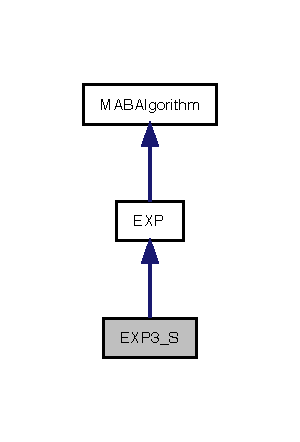
\includegraphics[width=144pt]{class_e_x_p3___s__inherit__graph}
\end{center}
\end{figure}


Collaboration diagram for E\+X\+P3\+\_\+S\+:
\nopagebreak
\begin{figure}[H]
\begin{center}
\leavevmode
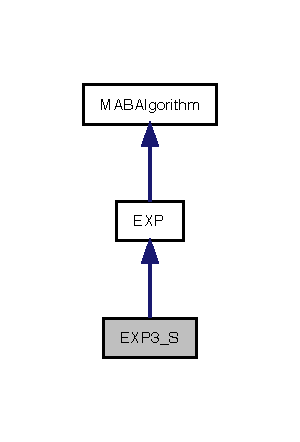
\includegraphics[width=144pt]{class_e_x_p3___s__coll__graph}
\end{center}
\end{figure}
\subsection*{Public Member Functions}
\begin{DoxyCompactItemize}
\item 
\mbox{\hyperlink{class_e_x_p3___s_ac5cd1864b3f23afbc5876a291c2a16d1}{E\+X\+P3\+\_\+S}} (string \mbox{\hyperlink{class_m_a_b_algorithm_a77b10ecc4b49d519c557f65358167b82}{name}}, int \mbox{\hyperlink{class_m_a_b_algorithm_a340fa9e83e85b092f2c6125fc4e8549b}{num\+\_\+of\+\_\+arms}}, double beta, double alpha)
\begin{DoxyCompactList}\small\item\em constructor of \mbox{\hyperlink{class_e_x_p3___s}{E\+X\+P3\+\_\+S}} \end{DoxyCompactList}\item 
int \mbox{\hyperlink{class_e_x_p3___s_afc9e4825004f5f541f774ac0debe6bee}{choose\+\_\+action}} () override
\item 
void \mbox{\hyperlink{class_e_x_p3___s_a93cef92a4f0213f7d247768b610071ad}{receive\+\_\+reward}} (double reward, int pulled\+\_\+arm) override
\begin{DoxyCompactList}\small\item\em Update the internal variables of the algorithm according to the new received reward. \end{DoxyCompactList}\item 
void \mbox{\hyperlink{class_e_x_p3___s_a70bfd4fc19a73ab7d2903672c36b2765}{reset}} (int action=-\/1) override
\begin{DoxyCompactList}\small\item\em resets the internal variables of the algorithm \end{DoxyCompactList}\end{DoxyCompactItemize}
\subsection*{Additional Inherited Members}


\subsection{Detailed Description}
\mbox{\hyperlink{class_e_x_p3___s}{E\+X\+P3\+\_\+S}} algorithm. 

\subsection{Constructor \& Destructor Documentation}
\mbox{\Hypertarget{class_e_x_p3___s_ac5cd1864b3f23afbc5876a291c2a16d1}\label{class_e_x_p3___s_ac5cd1864b3f23afbc5876a291c2a16d1}} 
\index{E\+X\+P3\+\_\+S@{E\+X\+P3\+\_\+S}!E\+X\+P3\+\_\+S@{E\+X\+P3\+\_\+S}}
\index{E\+X\+P3\+\_\+S@{E\+X\+P3\+\_\+S}!E\+X\+P3\+\_\+S@{E\+X\+P3\+\_\+S}}
\subsubsection{\texorpdfstring{E\+X\+P3\+\_\+\+S()}{EXP3\_S()}}
{\footnotesize\ttfamily E\+X\+P3\+\_\+\+S\+::\+E\+X\+P3\+\_\+S (\begin{DoxyParamCaption}\item[{string}]{name,  }\item[{int}]{num\+\_\+of\+\_\+arms,  }\item[{double}]{beta,  }\item[{double}]{alpha }\end{DoxyParamCaption})}



constructor of \mbox{\hyperlink{class_e_x_p3___s}{E\+X\+P3\+\_\+S}} 


\begin{DoxyParams}{Parameters}
{\em name} & string, id of the algorithm \\
\hline
{\em num\+\_\+of\+\_\+arms} & integer, number of arms the algorithm will work on \\
\hline
{\em beta} & double, exploration parameter (between 0 and 1) and also exponential update parameter \\
\hline
{\em alpha} & double, probability update parameter \\
\hline
\end{DoxyParams}


\subsection{Member Function Documentation}
\mbox{\Hypertarget{class_e_x_p3___s_afc9e4825004f5f541f774ac0debe6bee}\label{class_e_x_p3___s_afc9e4825004f5f541f774ac0debe6bee}} 
\index{E\+X\+P3\+\_\+S@{E\+X\+P3\+\_\+S}!choose\+\_\+action@{choose\+\_\+action}}
\index{choose\+\_\+action@{choose\+\_\+action}!E\+X\+P3\+\_\+S@{E\+X\+P3\+\_\+S}}
\subsubsection{\texorpdfstring{choose\+\_\+action()}{choose\_action()}}
{\footnotesize\ttfamily int E\+X\+P3\+\_\+\+S\+::choose\+\_\+action (\begin{DoxyParamCaption}{ }\end{DoxyParamCaption})\hspace{0.3cm}{\ttfamily [override]}, {\ttfamily [virtual]}}

\begin{DoxyReturn}{Returns}
an integer representing the chosen arm 
\end{DoxyReturn}


Implements \mbox{\hyperlink{class_m_a_b_algorithm_afb48f01df0e1860d19759f6e20335007}{M\+A\+B\+Algorithm}}.

\mbox{\Hypertarget{class_e_x_p3___s_a93cef92a4f0213f7d247768b610071ad}\label{class_e_x_p3___s_a93cef92a4f0213f7d247768b610071ad}} 
\index{E\+X\+P3\+\_\+S@{E\+X\+P3\+\_\+S}!receive\+\_\+reward@{receive\+\_\+reward}}
\index{receive\+\_\+reward@{receive\+\_\+reward}!E\+X\+P3\+\_\+S@{E\+X\+P3\+\_\+S}}
\subsubsection{\texorpdfstring{receive\+\_\+reward()}{receive\_reward()}}
{\footnotesize\ttfamily void E\+X\+P3\+\_\+\+S\+::receive\+\_\+reward (\begin{DoxyParamCaption}\item[{double}]{reward,  }\item[{int}]{pulled\+\_\+arm }\end{DoxyParamCaption})\hspace{0.3cm}{\ttfamily [override]}, {\ttfamily [virtual]}}



Update the internal variables of the algorithm according to the new received reward. 


\begin{DoxyParams}{Parameters}
{\em reward} & double, new received reward \\
\hline
{\em pulled\+\_\+arm} & integer, represents the pulled arm \\
\hline
\end{DoxyParams}


Reimplemented from \mbox{\hyperlink{class_m_a_b_algorithm_aa584b3d6b86fa050e3389be9781b5782}{M\+A\+B\+Algorithm}}.

\mbox{\Hypertarget{class_e_x_p3___s_a70bfd4fc19a73ab7d2903672c36b2765}\label{class_e_x_p3___s_a70bfd4fc19a73ab7d2903672c36b2765}} 
\index{E\+X\+P3\+\_\+S@{E\+X\+P3\+\_\+S}!reset@{reset}}
\index{reset@{reset}!E\+X\+P3\+\_\+S@{E\+X\+P3\+\_\+S}}
\subsubsection{\texorpdfstring{reset()}{reset()}}
{\footnotesize\ttfamily void E\+X\+P3\+\_\+\+S\+::reset (\begin{DoxyParamCaption}\item[{int}]{action = {\ttfamily -\/1} }\end{DoxyParamCaption})\hspace{0.3cm}{\ttfamily [override]}, {\ttfamily [virtual]}}



resets the internal variables of the algorithm 


\begin{DoxyParams}{Parameters}
{\em action} & integer, specifies which variables to reset. If in (0, num\+\_\+of\+\_\+arms -\/ 1), then it resets only the info related to such arm. If == -\/1, resets all the arms. \\
\hline
\end{DoxyParams}


Reimplemented from \mbox{\hyperlink{class_m_a_b_algorithm_ad5761cee0b0e3421d1f043dbcc0b5f85}{M\+A\+B\+Algorithm}}.



The documentation for this class was generated from the following files\+:\begin{DoxyCompactItemize}
\item 
src/\mbox{\hyperlink{exp_8h}{exp.\+h}}\item 
src/\mbox{\hyperlink{exp_8cpp}{exp.\+cpp}}\end{DoxyCompactItemize}

\hypertarget{class_experiment}{}\section{Experiment Class Reference}
\label{class_experiment}\index{Experiment@{Experiment}}


Class that represent an experiment. An experiment is composed by a \mbox{\hyperlink{class_m_a_b}{M\+AB}} setting (i.\+e. a set of arms), a set of \mbox{\hyperlink{class_m_a_b_algorithm}{M\+A\+B\+Algorithm}} and a Regret\+Type, which specifies the type of regret we are insterest into.  




{\ttfamily \#include $<$experiment.\+h$>$}

\subsection*{Public Member Functions}
\begin{DoxyCompactItemize}
\item 
\mbox{\hyperlink{class_experiment_ac89f5aa94daeec555004535271d36a17}{Experiment}} (string \mbox{\hyperlink{class_experiment_a2e451e5a87839f29986a54bf69715a79}{name}}, int \mbox{\hyperlink{class_experiment_ad95d4677faced6cf6b2d1f037f07901a}{num\+\_\+simulations}}, int \mbox{\hyperlink{class_experiment_a380452065b55d8e50a95b4f3608a80ca}{timesteps}}, int \mbox{\hyperlink{class_experiment_a5afc2955f4e99280fe0f4e8023582aec}{seed}})
\begin{DoxyCompactList}\small\item\em Constructor for \mbox{\hyperlink{class_experiment}{Experiment}}. \end{DoxyCompactList}\item 
void \mbox{\hyperlink{class_experiment_a7529561ca5ec4f7d1cd9b91bec8bd669}{set\+\_\+mab}} (\mbox{\hyperlink{class_m_a_b_experiment}{M\+A\+B\+Experiment}} $\ast$mab)
\begin{DoxyCompactList}\small\item\em Set the \mbox{\hyperlink{class_m_a_b}{M\+AB}} of this experiment according to the builder pattern. \end{DoxyCompactList}\item 
void \mbox{\hyperlink{class_experiment_ab2c105c70a67a5bed51b5d83c3b61e18}{set\+\_\+mab\+\_\+type}} (\mbox{\hyperlink{mab_8h_ab8d3b06b9f83219c5bb8daa68136f908}{Regret\+Type}} mabtype)
\begin{DoxyCompactList}\small\item\em Set the Regret\+Type of this experiment according to the builder pattern. \end{DoxyCompactList}\item 
void \mbox{\hyperlink{class_experiment_a0baf82bc31099824ce92d33899c78702}{add\+\_\+alg}} (\mbox{\hyperlink{class_m_a_b_algorithm}{M\+A\+B\+Algorithm}} $\ast$alg)
\begin{DoxyCompactList}\small\item\em Add a new \mbox{\hyperlink{class_m_a_b_algorithm}{M\+A\+B\+Algorithm}} to this experiment according to the builder pattern. \end{DoxyCompactList}\item 
void \mbox{\hyperlink{class_experiment_ac3467eb067f8623c9cf3cd7c736a8c80}{run}} ()
\begin{DoxyCompactList}\small\item\em Runs the experiment. It requires the \mbox{\hyperlink{class_m_a_b}{M\+AB}}, M\+A\+B\+Algorithms and Regret\+Type to be already set. It creates a \mbox{\hyperlink{class_statistic_manager}{Statistic\+Manager}} and uses it to store data about the experiment in some files in the temp directory. \end{DoxyCompactList}\end{DoxyCompactItemize}
\subsection*{Public Attributes}
\begin{DoxyCompactItemize}
\item 
string \mbox{\hyperlink{class_experiment_a2e451e5a87839f29986a54bf69715a79}{name}}
\item 
int \mbox{\hyperlink{class_experiment_ad95d4677faced6cf6b2d1f037f07901a}{num\+\_\+simulations}}
\item 
int \mbox{\hyperlink{class_experiment_a380452065b55d8e50a95b4f3608a80ca}{timesteps}}
\item 
int \mbox{\hyperlink{class_experiment_a5afc2955f4e99280fe0f4e8023582aec}{seed}}
\end{DoxyCompactItemize}


\subsection{Detailed Description}
Class that represent an experiment. An experiment is composed by a \mbox{\hyperlink{class_m_a_b}{M\+AB}} setting (i.\+e. a set of arms), a set of \mbox{\hyperlink{class_m_a_b_algorithm}{M\+A\+B\+Algorithm}} and a Regret\+Type, which specifies the type of regret we are insterest into. 

\subsection{Constructor \& Destructor Documentation}
\mbox{\Hypertarget{class_experiment_ac89f5aa94daeec555004535271d36a17}\label{class_experiment_ac89f5aa94daeec555004535271d36a17}} 
\index{Experiment@{Experiment}!Experiment@{Experiment}}
\index{Experiment@{Experiment}!Experiment@{Experiment}}
\subsubsection{\texorpdfstring{Experiment()}{Experiment()}}
{\footnotesize\ttfamily Experiment\+::\+Experiment (\begin{DoxyParamCaption}\item[{string}]{name,  }\item[{int}]{num\+\_\+simulations,  }\item[{int}]{timesteps,  }\item[{int}]{seed }\end{DoxyParamCaption})}



Constructor for \mbox{\hyperlink{class_experiment}{Experiment}}. 


\begin{DoxyParams}{Parameters}
{\em name} & string, used to identify the experiment \\
\hline
{\em num\+\_\+simulations} & int, represents the number of times the experiment is run with a different seed \\
\hline
{\em timestep} & int, the time horizon of the experiment \\
\hline
{\em seed} & int, the seed with which the first simulation of the experiment starts. \\
\hline
\end{DoxyParams}
\begin{DoxyReturn}{Returns}
an instance of \mbox{\hyperlink{class_experiment}{Experiment}} 
\end{DoxyReturn}


\subsection{Member Function Documentation}
\mbox{\Hypertarget{class_experiment_a0baf82bc31099824ce92d33899c78702}\label{class_experiment_a0baf82bc31099824ce92d33899c78702}} 
\index{Experiment@{Experiment}!add\+\_\+alg@{add\+\_\+alg}}
\index{add\+\_\+alg@{add\+\_\+alg}!Experiment@{Experiment}}
\subsubsection{\texorpdfstring{add\+\_\+alg()}{add\_alg()}}
{\footnotesize\ttfamily void Experiment\+::add\+\_\+alg (\begin{DoxyParamCaption}\item[{\mbox{\hyperlink{class_m_a_b_algorithm}{M\+A\+B\+Algorithm}} $\ast$}]{alg }\end{DoxyParamCaption})}



Add a new \mbox{\hyperlink{class_m_a_b_algorithm}{M\+A\+B\+Algorithm}} to this experiment according to the builder pattern. 


\begin{DoxyParams}{Parameters}
{\em alg} & \mbox{\hyperlink{class_m_a_b_algorithm}{M\+A\+B\+Algorithm}} that will be added to the experiment \\
\hline
\end{DoxyParams}
\begin{DoxyReturn}{Returns}
nothing 
\end{DoxyReturn}
\mbox{\Hypertarget{class_experiment_ac3467eb067f8623c9cf3cd7c736a8c80}\label{class_experiment_ac3467eb067f8623c9cf3cd7c736a8c80}} 
\index{Experiment@{Experiment}!run@{run}}
\index{run@{run}!Experiment@{Experiment}}
\subsubsection{\texorpdfstring{run()}{run()}}
{\footnotesize\ttfamily void Experiment\+::run (\begin{DoxyParamCaption}{ }\end{DoxyParamCaption})}



Runs the experiment. It requires the \mbox{\hyperlink{class_m_a_b}{M\+AB}}, M\+A\+B\+Algorithms and Regret\+Type to be already set. It creates a \mbox{\hyperlink{class_statistic_manager}{Statistic\+Manager}} and uses it to store data about the experiment in some files in the temp directory. 

\begin{DoxyReturn}{Returns}
nothing 
\end{DoxyReturn}
\mbox{\Hypertarget{class_experiment_a7529561ca5ec4f7d1cd9b91bec8bd669}\label{class_experiment_a7529561ca5ec4f7d1cd9b91bec8bd669}} 
\index{Experiment@{Experiment}!set\+\_\+mab@{set\+\_\+mab}}
\index{set\+\_\+mab@{set\+\_\+mab}!Experiment@{Experiment}}
\subsubsection{\texorpdfstring{set\+\_\+mab()}{set\_mab()}}
{\footnotesize\ttfamily void Experiment\+::set\+\_\+mab (\begin{DoxyParamCaption}\item[{\mbox{\hyperlink{class_m_a_b_experiment}{M\+A\+B\+Experiment}} $\ast$}]{mab }\end{DoxyParamCaption})}



Set the \mbox{\hyperlink{class_m_a_b}{M\+AB}} of this experiment according to the builder pattern. 


\begin{DoxyParams}{Parameters}
{\em mab} & \mbox{\hyperlink{class_m_a_b}{M\+AB}} used by the experiment. \\
\hline
\end{DoxyParams}
\begin{DoxyReturn}{Returns}
nothing 
\end{DoxyReturn}
\mbox{\Hypertarget{class_experiment_ab2c105c70a67a5bed51b5d83c3b61e18}\label{class_experiment_ab2c105c70a67a5bed51b5d83c3b61e18}} 
\index{Experiment@{Experiment}!set\+\_\+mab\+\_\+type@{set\+\_\+mab\+\_\+type}}
\index{set\+\_\+mab\+\_\+type@{set\+\_\+mab\+\_\+type}!Experiment@{Experiment}}
\subsubsection{\texorpdfstring{set\+\_\+mab\+\_\+type()}{set\_mab\_type()}}
{\footnotesize\ttfamily void Experiment\+::set\+\_\+mab\+\_\+type (\begin{DoxyParamCaption}\item[{\mbox{\hyperlink{mab_8h_ab8d3b06b9f83219c5bb8daa68136f908}{Regret\+Type}}}]{mabtype }\end{DoxyParamCaption})}



Set the Regret\+Type of this experiment according to the builder pattern. 


\begin{DoxyParams}{Parameters}
{\em mabtype} & the Regret\+Type of this experiment \\
\hline
\end{DoxyParams}
\begin{DoxyReturn}{Returns}
nothing 
\end{DoxyReturn}


\subsection{Member Data Documentation}
\mbox{\Hypertarget{class_experiment_a2e451e5a87839f29986a54bf69715a79}\label{class_experiment_a2e451e5a87839f29986a54bf69715a79}} 
\index{Experiment@{Experiment}!name@{name}}
\index{name@{name}!Experiment@{Experiment}}
\subsubsection{\texorpdfstring{name}{name}}
{\footnotesize\ttfamily string Experiment\+::name}

\mbox{\Hypertarget{class_experiment_ad95d4677faced6cf6b2d1f037f07901a}\label{class_experiment_ad95d4677faced6cf6b2d1f037f07901a}} 
\index{Experiment@{Experiment}!num\+\_\+simulations@{num\+\_\+simulations}}
\index{num\+\_\+simulations@{num\+\_\+simulations}!Experiment@{Experiment}}
\subsubsection{\texorpdfstring{num\+\_\+simulations}{num\_simulations}}
{\footnotesize\ttfamily int Experiment\+::num\+\_\+simulations}

\mbox{\Hypertarget{class_experiment_a5afc2955f4e99280fe0f4e8023582aec}\label{class_experiment_a5afc2955f4e99280fe0f4e8023582aec}} 
\index{Experiment@{Experiment}!seed@{seed}}
\index{seed@{seed}!Experiment@{Experiment}}
\subsubsection{\texorpdfstring{seed}{seed}}
{\footnotesize\ttfamily int Experiment\+::seed}

\mbox{\Hypertarget{class_experiment_a380452065b55d8e50a95b4f3608a80ca}\label{class_experiment_a380452065b55d8e50a95b4f3608a80ca}} 
\index{Experiment@{Experiment}!timesteps@{timesteps}}
\index{timesteps@{timesteps}!Experiment@{Experiment}}
\subsubsection{\texorpdfstring{timesteps}{timesteps}}
{\footnotesize\ttfamily int Experiment\+::timesteps}



The documentation for this class was generated from the following files\+:\begin{DoxyCompactItemize}
\item 
src/\mbox{\hyperlink{experiment_8h}{experiment.\+h}}\item 
src/\mbox{\hyperlink{experiment_8cpp}{experiment.\+cpp}}\end{DoxyCompactItemize}

\hypertarget{class_experiment_loader}{}\section{Experiment\+Loader Class Reference}
\label{class_experiment_loader}\index{Experiment\+Loader@{Experiment\+Loader}}


class whose main goal is to offer a static method which returns a vector of experiments loaded from a configuration file.  




{\ttfamily \#include $<$experimentloader.\+h$>$}

\subsection*{Static Public Member Functions}
\begin{DoxyCompactItemize}
\item 
static vector$<$ \mbox{\hyperlink{class_experiment}{Experiment}} $\ast$ $>$ $\ast$ \mbox{\hyperlink{class_experiment_loader_a1884a60d8ebc82544600e91c37fbc831}{load\+\_\+experiments}} ()
\end{DoxyCompactItemize}


\subsection{Detailed Description}
class whose main goal is to offer a static method which returns a vector of experiments loaded from a configuration file. 

\subsection{Member Function Documentation}
\mbox{\Hypertarget{class_experiment_loader_a1884a60d8ebc82544600e91c37fbc831}\label{class_experiment_loader_a1884a60d8ebc82544600e91c37fbc831}} 
\index{Experiment\+Loader@{Experiment\+Loader}!load\+\_\+experiments@{load\+\_\+experiments}}
\index{load\+\_\+experiments@{load\+\_\+experiments}!Experiment\+Loader@{Experiment\+Loader}}
\subsubsection{\texorpdfstring{load\+\_\+experiments()}{load\_experiments()}}
{\footnotesize\ttfamily vector$<$ \mbox{\hyperlink{class_experiment}{Experiment}} $\ast$ $>$ $\ast$ Experiment\+Loader\+::load\+\_\+experiments (\begin{DoxyParamCaption}{ }\end{DoxyParamCaption})\hspace{0.3cm}{\ttfamily [static]}}

\begin{DoxyReturn}{Returns}
a vector of experiments loaded from a configuration file. 
\end{DoxyReturn}


The documentation for this class was generated from the following files\+:\begin{DoxyCompactItemize}
\item 
src/\mbox{\hyperlink{experimentloader_8h}{experimentloader.\+h}}\item 
src/\mbox{\hyperlink{experimentloader_8cpp}{experimentloader.\+cpp}}\end{DoxyCompactItemize}

\hypertarget{class_fixed_distribution}{}\section{Fixed\+Distribution Class Reference}
\label{class_fixed_distribution}\index{Fixed\+Distribution@{Fixed\+Distribution}}


\mbox{\hyperlink{class_distribution}{Distribution}} of a fixed distribution, i.\+e. it returns always the same value.  




{\ttfamily \#include $<$distribution.\+h$>$}



Inheritance diagram for Fixed\+Distribution\+:
\nopagebreak
\begin{figure}[H]
\begin{center}
\leavevmode
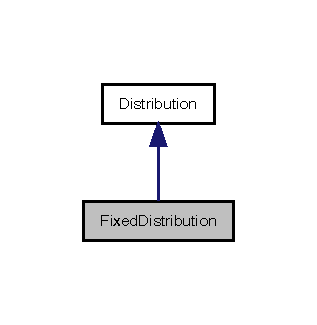
\includegraphics[width=152pt]{class_fixed_distribution__inherit__graph}
\end{center}
\end{figure}


Collaboration diagram for Fixed\+Distribution\+:
\nopagebreak
\begin{figure}[H]
\begin{center}
\leavevmode
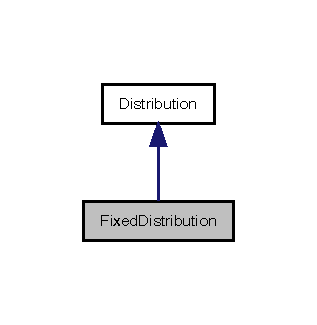
\includegraphics[width=152pt]{class_fixed_distribution__coll__graph}
\end{center}
\end{figure}
\subsection*{Public Member Functions}
\begin{DoxyCompactItemize}
\item 
\mbox{\hyperlink{class_fixed_distribution_acdcfb34ebf33609d6ce7bdacff9a34d8}{Fixed\+Distribution}} (string \mbox{\hyperlink{class_distribution_ab3b7be02f0401cb76beb2e744b6161f9}{name}}, double v, boost\+::mt19937 \&\mbox{\hyperlink{class_distribution_ac8915a45ce85ab6b7506fa42bb850a89}{rng}})
\item 
double \mbox{\hyperlink{class_fixed_distribution_a1babd43b5bbc4e0a720ca77690c9adad}{draw}} (int timestep) override
\item 
string \mbox{\hyperlink{class_fixed_distribution_a6396ce831e3ff31ecc39bda45e3ecb08}{to\+File}} () override
\begin{DoxyCompactList}\small\item\em build a representation of this \mbox{\hyperlink{class_distribution}{Distribution}} so that it can be printed to a file and be later analysed by another script \end{DoxyCompactList}\item 
double \mbox{\hyperlink{class_fixed_distribution_af9199f9076551694af2397c7dd69096e}{get\+\_\+mean}} (int timestep) override
\end{DoxyCompactItemize}
\subsection*{Additional Inherited Members}


\subsection{Detailed Description}
\mbox{\hyperlink{class_distribution}{Distribution}} of a fixed distribution, i.\+e. it returns always the same value. 


\begin{DoxyParams}{Parameters}
{\em name} & string, id of the distribution \\
\hline
{\em v} & double, the value always returned by the distribution \\
\hline
{\em rng} & boost\+::mt19937\&, rng used to generate data \\
\hline
\end{DoxyParams}


\subsection{Constructor \& Destructor Documentation}
\mbox{\Hypertarget{class_fixed_distribution_acdcfb34ebf33609d6ce7bdacff9a34d8}\label{class_fixed_distribution_acdcfb34ebf33609d6ce7bdacff9a34d8}} 
\index{Fixed\+Distribution@{Fixed\+Distribution}!Fixed\+Distribution@{Fixed\+Distribution}}
\index{Fixed\+Distribution@{Fixed\+Distribution}!Fixed\+Distribution@{Fixed\+Distribution}}
\subsubsection{\texorpdfstring{Fixed\+Distribution()}{FixedDistribution()}}
{\footnotesize\ttfamily Fixed\+Distribution\+::\+Fixed\+Distribution (\begin{DoxyParamCaption}\item[{string}]{name,  }\item[{double}]{v,  }\item[{boost\+::mt19937 \&}]{rng }\end{DoxyParamCaption})}


\begin{DoxyParams}{Parameters}
{\em name} & string, id of the distribution \\
\hline
{\em v} & double, the value always returned by the distribution \\
\hline
{\em rng} & boost\+::mt19937\&, rng used to generate data \\
\hline
\end{DoxyParams}


\subsection{Member Function Documentation}
\mbox{\Hypertarget{class_fixed_distribution_a1babd43b5bbc4e0a720ca77690c9adad}\label{class_fixed_distribution_a1babd43b5bbc4e0a720ca77690c9adad}} 
\index{Fixed\+Distribution@{Fixed\+Distribution}!draw@{draw}}
\index{draw@{draw}!Fixed\+Distribution@{Fixed\+Distribution}}
\subsubsection{\texorpdfstring{draw()}{draw()}}
{\footnotesize\ttfamily double Fixed\+Distribution\+::draw (\begin{DoxyParamCaption}\item[{int}]{timestep }\end{DoxyParamCaption})\hspace{0.3cm}{\ttfamily [override]}, {\ttfamily [virtual]}}


\begin{DoxyParams}{Parameters}
{\em timestep} & int, timestep at which the reward is drawn \\
\hline
\end{DoxyParams}
\begin{DoxyReturn}{Returns}
a double which is the drawn reward 
\end{DoxyReturn}


Implements \mbox{\hyperlink{class_distribution_a742b398af4a461243028cce3c47d8080}{Distribution}}.

\mbox{\Hypertarget{class_fixed_distribution_af9199f9076551694af2397c7dd69096e}\label{class_fixed_distribution_af9199f9076551694af2397c7dd69096e}} 
\index{Fixed\+Distribution@{Fixed\+Distribution}!get\+\_\+mean@{get\+\_\+mean}}
\index{get\+\_\+mean@{get\+\_\+mean}!Fixed\+Distribution@{Fixed\+Distribution}}
\subsubsection{\texorpdfstring{get\+\_\+mean()}{get\_mean()}}
{\footnotesize\ttfamily double Fixed\+Distribution\+::get\+\_\+mean (\begin{DoxyParamCaption}\item[{int}]{timestep }\end{DoxyParamCaption})\hspace{0.3cm}{\ttfamily [override]}, {\ttfamily [virtual]}}


\begin{DoxyParams}{Parameters}
{\em timestep} & integer, the timestep at which the mean is asked \\
\hline
\end{DoxyParams}
\begin{DoxyReturn}{Returns}
the mean (double) at the specified timestep 
\end{DoxyReturn}


Implements \mbox{\hyperlink{class_distribution_ac9c74d18549f532caa09ae86d8b25b55}{Distribution}}.

\mbox{\Hypertarget{class_fixed_distribution_a6396ce831e3ff31ecc39bda45e3ecb08}\label{class_fixed_distribution_a6396ce831e3ff31ecc39bda45e3ecb08}} 
\index{Fixed\+Distribution@{Fixed\+Distribution}!to\+File@{to\+File}}
\index{to\+File@{to\+File}!Fixed\+Distribution@{Fixed\+Distribution}}
\subsubsection{\texorpdfstring{to\+File()}{toFile()}}
{\footnotesize\ttfamily string Fixed\+Distribution\+::to\+File (\begin{DoxyParamCaption}{ }\end{DoxyParamCaption})\hspace{0.3cm}{\ttfamily [override]}, {\ttfamily [virtual]}}



build a representation of this \mbox{\hyperlink{class_distribution}{Distribution}} so that it can be printed to a file and be later analysed by another script 

\begin{DoxyReturn}{Returns}
a string that represents this \mbox{\hyperlink{class_distribution}{Distribution}} 
\end{DoxyReturn}


Implements \mbox{\hyperlink{class_distribution_ac41d57a4d7f82041810f886590a236a5}{Distribution}}.



The documentation for this class was generated from the following files\+:\begin{DoxyCompactItemize}
\item 
src/\mbox{\hyperlink{distribution_8h}{distribution.\+h}}\item 
src/\mbox{\hyperlink{distribution_8cpp}{distribution.\+cpp}}\end{DoxyCompactItemize}

\hypertarget{class_fixed_non_stationary_distribution}{}\section{Fixed\+Non\+Stationary\+Distribution Class Reference}
\label{class_fixed_non_stationary_distribution}\index{Fixed\+Non\+Stationary\+Distribution@{Fixed\+Non\+Stationary\+Distribution}}


\mbox{\hyperlink{class_distribution}{Distribution}} of a non-\/stationary fixed distribution, i.\+e. it returns always the same value inside the same slot.  




{\ttfamily \#include $<$distribution.\+h$>$}



Inheritance diagram for Fixed\+Non\+Stationary\+Distribution\+:
\nopagebreak
\begin{figure}[H]
\begin{center}
\leavevmode
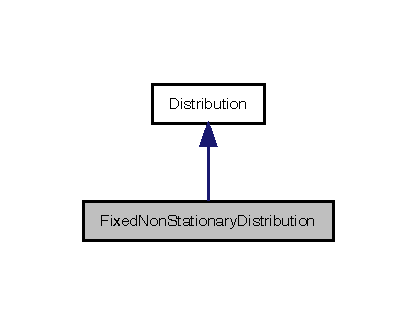
\includegraphics[width=200pt]{class_fixed_non_stationary_distribution__inherit__graph}
\end{center}
\end{figure}


Collaboration diagram for Fixed\+Non\+Stationary\+Distribution\+:
\nopagebreak
\begin{figure}[H]
\begin{center}
\leavevmode
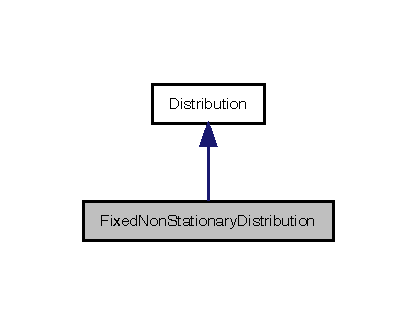
\includegraphics[width=200pt]{class_fixed_non_stationary_distribution__coll__graph}
\end{center}
\end{figure}
\subsection*{Public Member Functions}
\begin{DoxyCompactItemize}
\item 
\mbox{\hyperlink{class_fixed_non_stationary_distribution_ada03636450043064e36d00e70d479788}{Fixed\+Non\+Stationary\+Distribution}} (string \mbox{\hyperlink{class_distribution_ab3b7be02f0401cb76beb2e744b6161f9}{name}}, vector$<$ double $>$ \&vs, vector$<$ int $>$ ends, boost\+::mt19937 \&\mbox{\hyperlink{class_distribution_ac8915a45ce85ab6b7506fa42bb850a89}{rng}})
\item 
double \mbox{\hyperlink{class_fixed_non_stationary_distribution_afd4a118bfe398f700e93430ca05dbae6}{draw}} (int timestep) override
\item 
string \mbox{\hyperlink{class_fixed_non_stationary_distribution_aaea49214758451b31f83a272af1626e0}{to\+File}} () override
\begin{DoxyCompactList}\small\item\em build a representation of this \mbox{\hyperlink{class_distribution}{Distribution}} so that it can be printed to a file and be later analysed by another script \end{DoxyCompactList}\item 
double \mbox{\hyperlink{class_fixed_non_stationary_distribution_aa9ed51fbf731f288a76a3a9e0aee8390}{get\+\_\+mean}} (int timestep) override
\end{DoxyCompactItemize}
\subsection*{Additional Inherited Members}


\subsection{Detailed Description}
\mbox{\hyperlink{class_distribution}{Distribution}} of a non-\/stationary fixed distribution, i.\+e. it returns always the same value inside the same slot. 


\begin{DoxyParams}{Parameters}
{\em name} & string, id of the distribution \\
\hline
{\em vs} & vector$<$double$>$\&, the values always returned by the distribution in the time slots \\
\hline
{\em ends} & vector$<$double$>$\&, the last timestep of each time slot \\
\hline
{\em rng} & boost\+::mt19937\&, rng used to generate data \\
\hline
\end{DoxyParams}


\subsection{Constructor \& Destructor Documentation}
\mbox{\Hypertarget{class_fixed_non_stationary_distribution_ada03636450043064e36d00e70d479788}\label{class_fixed_non_stationary_distribution_ada03636450043064e36d00e70d479788}} 
\index{Fixed\+Non\+Stationary\+Distribution@{Fixed\+Non\+Stationary\+Distribution}!Fixed\+Non\+Stationary\+Distribution@{Fixed\+Non\+Stationary\+Distribution}}
\index{Fixed\+Non\+Stationary\+Distribution@{Fixed\+Non\+Stationary\+Distribution}!Fixed\+Non\+Stationary\+Distribution@{Fixed\+Non\+Stationary\+Distribution}}
\subsubsection{\texorpdfstring{Fixed\+Non\+Stationary\+Distribution()}{FixedNonStationaryDistribution()}}
{\footnotesize\ttfamily Fixed\+Non\+Stationary\+Distribution\+::\+Fixed\+Non\+Stationary\+Distribution (\begin{DoxyParamCaption}\item[{string}]{name,  }\item[{vector$<$ double $>$ \&}]{vs,  }\item[{vector$<$ int $>$}]{ends,  }\item[{boost\+::mt19937 \&}]{rng }\end{DoxyParamCaption})}


\begin{DoxyParams}{Parameters}
{\em name} & string, id of the distribution \\
\hline
{\em vs} & vector$<$double$>$\&, the values always returned by the distribution in the time slots \\
\hline
{\em ends} & vector$<$double$>$\&, the last timestep of each time slot \\
\hline
{\em rng} & boost\+::mt19937\&, rng used to generate data \\
\hline
\end{DoxyParams}


\subsection{Member Function Documentation}
\mbox{\Hypertarget{class_fixed_non_stationary_distribution_afd4a118bfe398f700e93430ca05dbae6}\label{class_fixed_non_stationary_distribution_afd4a118bfe398f700e93430ca05dbae6}} 
\index{Fixed\+Non\+Stationary\+Distribution@{Fixed\+Non\+Stationary\+Distribution}!draw@{draw}}
\index{draw@{draw}!Fixed\+Non\+Stationary\+Distribution@{Fixed\+Non\+Stationary\+Distribution}}
\subsubsection{\texorpdfstring{draw()}{draw()}}
{\footnotesize\ttfamily double Fixed\+Non\+Stationary\+Distribution\+::draw (\begin{DoxyParamCaption}\item[{int}]{timestep }\end{DoxyParamCaption})\hspace{0.3cm}{\ttfamily [override]}, {\ttfamily [virtual]}}


\begin{DoxyParams}{Parameters}
{\em timestep} & int, timestep at which the reward is drawn \\
\hline
\end{DoxyParams}
\begin{DoxyReturn}{Returns}
a double which is the drawn reward 
\end{DoxyReturn}


Implements \mbox{\hyperlink{class_distribution_a742b398af4a461243028cce3c47d8080}{Distribution}}.

\mbox{\Hypertarget{class_fixed_non_stationary_distribution_aa9ed51fbf731f288a76a3a9e0aee8390}\label{class_fixed_non_stationary_distribution_aa9ed51fbf731f288a76a3a9e0aee8390}} 
\index{Fixed\+Non\+Stationary\+Distribution@{Fixed\+Non\+Stationary\+Distribution}!get\+\_\+mean@{get\+\_\+mean}}
\index{get\+\_\+mean@{get\+\_\+mean}!Fixed\+Non\+Stationary\+Distribution@{Fixed\+Non\+Stationary\+Distribution}}
\subsubsection{\texorpdfstring{get\+\_\+mean()}{get\_mean()}}
{\footnotesize\ttfamily double Fixed\+Non\+Stationary\+Distribution\+::get\+\_\+mean (\begin{DoxyParamCaption}\item[{int}]{timestep }\end{DoxyParamCaption})\hspace{0.3cm}{\ttfamily [override]}, {\ttfamily [virtual]}}


\begin{DoxyParams}{Parameters}
{\em timestep} & integer, the timestep at which the mean is asked \\
\hline
\end{DoxyParams}
\begin{DoxyReturn}{Returns}
the mean (double) at the specified timestep 
\end{DoxyReturn}


Implements \mbox{\hyperlink{class_distribution_ac9c74d18549f532caa09ae86d8b25b55}{Distribution}}.

\mbox{\Hypertarget{class_fixed_non_stationary_distribution_aaea49214758451b31f83a272af1626e0}\label{class_fixed_non_stationary_distribution_aaea49214758451b31f83a272af1626e0}} 
\index{Fixed\+Non\+Stationary\+Distribution@{Fixed\+Non\+Stationary\+Distribution}!to\+File@{to\+File}}
\index{to\+File@{to\+File}!Fixed\+Non\+Stationary\+Distribution@{Fixed\+Non\+Stationary\+Distribution}}
\subsubsection{\texorpdfstring{to\+File()}{toFile()}}
{\footnotesize\ttfamily string Fixed\+Non\+Stationary\+Distribution\+::to\+File (\begin{DoxyParamCaption}{ }\end{DoxyParamCaption})\hspace{0.3cm}{\ttfamily [override]}, {\ttfamily [virtual]}}



build a representation of this \mbox{\hyperlink{class_distribution}{Distribution}} so that it can be printed to a file and be later analysed by another script 

\begin{DoxyReturn}{Returns}
a string that represents this \mbox{\hyperlink{class_distribution}{Distribution}} 
\end{DoxyReturn}


Implements \mbox{\hyperlink{class_distribution_ac41d57a4d7f82041810f886590a236a5}{Distribution}}.



The documentation for this class was generated from the following files\+:\begin{DoxyCompactItemize}
\item 
src/\mbox{\hyperlink{distribution_8h}{distribution.\+h}}\item 
src/\mbox{\hyperlink{distribution_8cpp}{distribution.\+cpp}}\end{DoxyCompactItemize}

\hypertarget{class_global_c_t_s}{}\section{Global\+C\+TS Class Reference}
\label{class_global_c_t_s}\index{Global\+C\+TS@{Global\+C\+TS}}


Thompson Sampling with prior on runlength distribution. \mbox{\hyperlink{class_distribution}{Distribution}} changes are assumed to happen globally (all the arms change at the same timestep)  




{\ttfamily \#include $<$thompsonsampling.\+h$>$}



Inheritance diagram for Global\+C\+TS\+:
\nopagebreak
\begin{figure}[H]
\begin{center}
\leavevmode
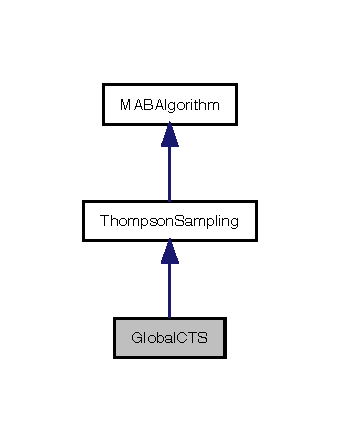
\includegraphics[width=163pt]{class_global_c_t_s__inherit__graph}
\end{center}
\end{figure}


Collaboration diagram for Global\+C\+TS\+:
\nopagebreak
\begin{figure}[H]
\begin{center}
\leavevmode
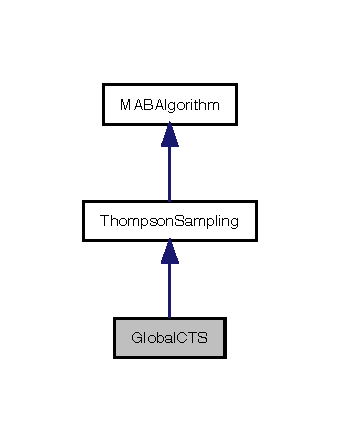
\includegraphics[width=163pt]{class_global_c_t_s__coll__graph}
\end{center}
\end{figure}
\subsection*{Public Member Functions}
\begin{DoxyCompactItemize}
\item 
\mbox{\hyperlink{class_global_c_t_s_a04fe6aa2e0a554e5e2e1edad47ecabe1}{Global\+C\+TS}} (string \mbox{\hyperlink{class_m_a_b_algorithm_a77b10ecc4b49d519c557f65358167b82}{name}}, int \mbox{\hyperlink{class_m_a_b_algorithm_a340fa9e83e85b092f2c6125fc4e8549b}{num\+\_\+of\+\_\+arms}}, boost\+::mt19937 \&\mbox{\hyperlink{class_thompson_sampling_a1b66efa9bb0912df92975147f8923216}{rng}}, double gamma)
\item 
int \mbox{\hyperlink{class_global_c_t_s_a48f9873be9f993e78fdbdd93ad4806bc}{choose\+\_\+action}} () override
\item 
void \mbox{\hyperlink{class_global_c_t_s_acb2f35fa8c6b2ae61912f6f337ed815f}{receive\+\_\+reward}} (double reward, int pulled\+\_\+arm) override
\begin{DoxyCompactList}\small\item\em Update the internal variables of the algorithm according to the new received reward. \end{DoxyCompactList}\item 
void \mbox{\hyperlink{class_global_c_t_s_a1e2c899b85ec7adf92a28ac758f556b5}{reset}} (int action=-\/1) override
\begin{DoxyCompactList}\small\item\em resets the internal variables of the algorithm \end{DoxyCompactList}\end{DoxyCompactItemize}
\subsection*{Additional Inherited Members}


\subsection{Detailed Description}
Thompson Sampling with prior on runlength distribution. \mbox{\hyperlink{class_distribution}{Distribution}} changes are assumed to happen globally (all the arms change at the same timestep) 

\subsection{Constructor \& Destructor Documentation}
\mbox{\Hypertarget{class_global_c_t_s_a04fe6aa2e0a554e5e2e1edad47ecabe1}\label{class_global_c_t_s_a04fe6aa2e0a554e5e2e1edad47ecabe1}} 
\index{Global\+C\+TS@{Global\+C\+TS}!Global\+C\+TS@{Global\+C\+TS}}
\index{Global\+C\+TS@{Global\+C\+TS}!Global\+C\+TS@{Global\+C\+TS}}
\subsubsection{\texorpdfstring{Global\+C\+T\+S()}{GlobalCTS()}}
{\footnotesize\ttfamily Global\+C\+T\+S\+::\+Global\+C\+TS (\begin{DoxyParamCaption}\item[{string}]{name,  }\item[{int}]{num\+\_\+of\+\_\+arms,  }\item[{boost\+::mt19937 \&}]{rng,  }\item[{double}]{gamma }\end{DoxyParamCaption})}


\begin{DoxyParams}{Parameters}
{\em name} & string, id of the algorithm \\
\hline
{\em num\+\_\+of\+\_\+arms} & integer, number of arms the algorithm will work on \\
\hline
{\em rng} & boost\+::mt19937\&, random number generator \\
\hline
{\em gamma} & double, parameter of the prior of the geometric runlength distribution \\
\hline
\end{DoxyParams}


\subsection{Member Function Documentation}
\mbox{\Hypertarget{class_global_c_t_s_a48f9873be9f993e78fdbdd93ad4806bc}\label{class_global_c_t_s_a48f9873be9f993e78fdbdd93ad4806bc}} 
\index{Global\+C\+TS@{Global\+C\+TS}!choose\+\_\+action@{choose\+\_\+action}}
\index{choose\+\_\+action@{choose\+\_\+action}!Global\+C\+TS@{Global\+C\+TS}}
\subsubsection{\texorpdfstring{choose\+\_\+action()}{choose\_action()}}
{\footnotesize\ttfamily int Global\+C\+T\+S\+::choose\+\_\+action (\begin{DoxyParamCaption}{ }\end{DoxyParamCaption})\hspace{0.3cm}{\ttfamily [override]}, {\ttfamily [virtual]}}

\begin{DoxyReturn}{Returns}
an integer representing the chosen arm 
\end{DoxyReturn}


Implements \mbox{\hyperlink{class_m_a_b_algorithm_afb48f01df0e1860d19759f6e20335007}{M\+A\+B\+Algorithm}}.

\mbox{\Hypertarget{class_global_c_t_s_acb2f35fa8c6b2ae61912f6f337ed815f}\label{class_global_c_t_s_acb2f35fa8c6b2ae61912f6f337ed815f}} 
\index{Global\+C\+TS@{Global\+C\+TS}!receive\+\_\+reward@{receive\+\_\+reward}}
\index{receive\+\_\+reward@{receive\+\_\+reward}!Global\+C\+TS@{Global\+C\+TS}}
\subsubsection{\texorpdfstring{receive\+\_\+reward()}{receive\_reward()}}
{\footnotesize\ttfamily void Global\+C\+T\+S\+::receive\+\_\+reward (\begin{DoxyParamCaption}\item[{double}]{reward,  }\item[{int}]{pulled\+\_\+arm }\end{DoxyParamCaption})\hspace{0.3cm}{\ttfamily [override]}, {\ttfamily [virtual]}}



Update the internal variables of the algorithm according to the new received reward. 


\begin{DoxyParams}{Parameters}
{\em reward} & double, new received reward \\
\hline
{\em pulled\+\_\+arm} & integer, represents the pulled arm \\
\hline
\end{DoxyParams}


Reimplemented from \mbox{\hyperlink{class_m_a_b_algorithm_aa584b3d6b86fa050e3389be9781b5782}{M\+A\+B\+Algorithm}}.

\mbox{\Hypertarget{class_global_c_t_s_a1e2c899b85ec7adf92a28ac758f556b5}\label{class_global_c_t_s_a1e2c899b85ec7adf92a28ac758f556b5}} 
\index{Global\+C\+TS@{Global\+C\+TS}!reset@{reset}}
\index{reset@{reset}!Global\+C\+TS@{Global\+C\+TS}}
\subsubsection{\texorpdfstring{reset()}{reset()}}
{\footnotesize\ttfamily void Global\+C\+T\+S\+::reset (\begin{DoxyParamCaption}\item[{int}]{action = {\ttfamily -\/1} }\end{DoxyParamCaption})\hspace{0.3cm}{\ttfamily [override]}, {\ttfamily [virtual]}}



resets the internal variables of the algorithm 


\begin{DoxyParams}{Parameters}
{\em action} & integer, specifies which variables to reset. If in (0, num\+\_\+of\+\_\+arms -\/ 1), then it resets only the info related to such arm. If == -\/1, resets all the arms. \\
\hline
\end{DoxyParams}


Reimplemented from \mbox{\hyperlink{class_m_a_b_algorithm_ad5761cee0b0e3421d1f043dbcc0b5f85}{M\+A\+B\+Algorithm}}.



The documentation for this class was generated from the following files\+:\begin{DoxyCompactItemize}
\item 
src/\mbox{\hyperlink{thompsonsampling_8h}{thompsonsampling.\+h}}\item 
src/\mbox{\hyperlink{thompsonsampling_8cpp}{thompsonsampling.\+cpp}}\end{DoxyCompactItemize}

\hypertarget{class_g_l_r}{}\section{G\+LR Class Reference}
\label{class_g_l_r}\index{G\+LR@{G\+LR}}


Meta-\/algorithm that selects at each timestep the sample history for its sub-\/algorithm using the Generalized Likelihood Ratio method.  




{\ttfamily \#include $<$meta\+\_\+algorithms.\+h$>$}



Inheritance diagram for G\+LR\+:
\nopagebreak
\begin{figure}[H]
\begin{center}
\leavevmode
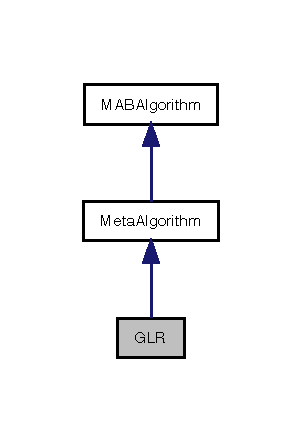
\includegraphics[width=145pt]{class_g_l_r__inherit__graph}
\end{center}
\end{figure}


Collaboration diagram for G\+LR\+:
\nopagebreak
\begin{figure}[H]
\begin{center}
\leavevmode
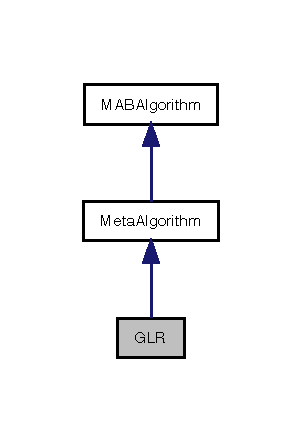
\includegraphics[width=145pt]{class_g_l_r__coll__graph}
\end{center}
\end{figure}
\subsection*{Public Member Functions}
\begin{DoxyCompactItemize}
\item 
\mbox{\hyperlink{class_g_l_r_a1f48d3cb0d12e111c1bafd9acae3da6b}{G\+LR}} (string \mbox{\hyperlink{class_m_a_b_algorithm_a77b10ecc4b49d519c557f65358167b82}{name}}, int \mbox{\hyperlink{class_m_a_b_algorithm_a340fa9e83e85b092f2c6125fc4e8549b}{num\+\_\+of\+\_\+arms}}, int M, int max\+\_\+history, string sub\+\_\+alg\+\_\+line, boost\+::mt19937 \&rng)
\item 
virtual int \mbox{\hyperlink{class_g_l_r_ad6b3e9f19e0bea4d6067b491c33640e0}{choose\+\_\+action}} () override
\item 
virtual void \mbox{\hyperlink{class_g_l_r_ad8e409518a110bd57f42a2de1b759707}{receive\+\_\+reward}} (double reward, int pulled\+\_\+arm) override
\begin{DoxyCompactList}\small\item\em Update the internal variables of the algorithm according to the new received reward. \end{DoxyCompactList}\item 
virtual void \mbox{\hyperlink{class_g_l_r_ad6c979e855b56e80ecfc54c8c93f035e}{reset}} (int action=-\/1) override
\begin{DoxyCompactList}\small\item\em resets the internal variables of the algorithm \end{DoxyCompactList}\end{DoxyCompactItemize}
\subsection*{Additional Inherited Members}


\subsection{Detailed Description}
Meta-\/algorithm that selects at each timestep the sample history for its sub-\/algorithm using the Generalized Likelihood Ratio method. 

\subsection{Constructor \& Destructor Documentation}
\mbox{\Hypertarget{class_g_l_r_a1f48d3cb0d12e111c1bafd9acae3da6b}\label{class_g_l_r_a1f48d3cb0d12e111c1bafd9acae3da6b}} 
\index{G\+LR@{G\+LR}!G\+LR@{G\+LR}}
\index{G\+LR@{G\+LR}!G\+LR@{G\+LR}}
\subsubsection{\texorpdfstring{G\+L\+R()}{GLR()}}
{\footnotesize\ttfamily G\+L\+R\+::\+G\+LR (\begin{DoxyParamCaption}\item[{string}]{name,  }\item[{int}]{num\+\_\+of\+\_\+arms,  }\item[{int}]{M,  }\item[{int}]{max\+\_\+history,  }\item[{string}]{sub\+\_\+alg\+\_\+line,  }\item[{boost\+::mt19937 \&}]{rng }\end{DoxyParamCaption})}


\begin{DoxyParams}{Parameters}
{\em name} & string, id of the algorithm \\
\hline
{\em num\+\_\+of\+\_\+arms} & integer, number of arms the algorithm will work with \\
\hline
{\em M} & integer, number of timesteps required by the \mbox{\hyperlink{class_c_d_t}{C\+DT}} to initialize itself \\
\hline
{\em max\+\_\+history} & integer, maximum amount of the latest samples that the algorithm scans for the most probable checkpoint \\
\hline
{\em sub\+\_\+alg\+\_\+line} & string, specification of the sub-\/algorithm \\
\hline
{\em rng} & boost\+::mt19937\&, random number generator \\
\hline
\end{DoxyParams}


\subsection{Member Function Documentation}
\mbox{\Hypertarget{class_g_l_r_ad6b3e9f19e0bea4d6067b491c33640e0}\label{class_g_l_r_ad6b3e9f19e0bea4d6067b491c33640e0}} 
\index{G\+LR@{G\+LR}!choose\+\_\+action@{choose\+\_\+action}}
\index{choose\+\_\+action@{choose\+\_\+action}!G\+LR@{G\+LR}}
\subsubsection{\texorpdfstring{choose\+\_\+action()}{choose\_action()}}
{\footnotesize\ttfamily int G\+L\+R\+::choose\+\_\+action (\begin{DoxyParamCaption}{ }\end{DoxyParamCaption})\hspace{0.3cm}{\ttfamily [override]}, {\ttfamily [virtual]}}

\begin{DoxyReturn}{Returns}
an integer representing the chosen arm 
\end{DoxyReturn}


Implements \mbox{\hyperlink{class_m_a_b_algorithm_afb48f01df0e1860d19759f6e20335007}{M\+A\+B\+Algorithm}}.

\mbox{\Hypertarget{class_g_l_r_ad8e409518a110bd57f42a2de1b759707}\label{class_g_l_r_ad8e409518a110bd57f42a2de1b759707}} 
\index{G\+LR@{G\+LR}!receive\+\_\+reward@{receive\+\_\+reward}}
\index{receive\+\_\+reward@{receive\+\_\+reward}!G\+LR@{G\+LR}}
\subsubsection{\texorpdfstring{receive\+\_\+reward()}{receive\_reward()}}
{\footnotesize\ttfamily void G\+L\+R\+::receive\+\_\+reward (\begin{DoxyParamCaption}\item[{double}]{reward,  }\item[{int}]{pulled\+\_\+arm }\end{DoxyParamCaption})\hspace{0.3cm}{\ttfamily [override]}, {\ttfamily [virtual]}}



Update the internal variables of the algorithm according to the new received reward. 


\begin{DoxyParams}{Parameters}
{\em reward} & double, new received reward \\
\hline
{\em pulled\+\_\+arm} & integer, represents the pulled arm \\
\hline
\end{DoxyParams}


Reimplemented from \mbox{\hyperlink{class_m_a_b_algorithm_aa584b3d6b86fa050e3389be9781b5782}{M\+A\+B\+Algorithm}}.

\mbox{\Hypertarget{class_g_l_r_ad6c979e855b56e80ecfc54c8c93f035e}\label{class_g_l_r_ad6c979e855b56e80ecfc54c8c93f035e}} 
\index{G\+LR@{G\+LR}!reset@{reset}}
\index{reset@{reset}!G\+LR@{G\+LR}}
\subsubsection{\texorpdfstring{reset()}{reset()}}
{\footnotesize\ttfamily void G\+L\+R\+::reset (\begin{DoxyParamCaption}\item[{int}]{action = {\ttfamily -\/1} }\end{DoxyParamCaption})\hspace{0.3cm}{\ttfamily [override]}, {\ttfamily [virtual]}}



resets the internal variables of the algorithm 


\begin{DoxyParams}{Parameters}
{\em action} & integer, specifies which variables to reset. If in (0, num\+\_\+of\+\_\+arms -\/ 1), then it resets only the info related to such arm. If == -\/1, resets all the arms. \\
\hline
\end{DoxyParams}


Reimplemented from \mbox{\hyperlink{class_m_a_b_algorithm_ad5761cee0b0e3421d1f043dbcc0b5f85}{M\+A\+B\+Algorithm}}.



The documentation for this class was generated from the following files\+:\begin{DoxyCompactItemize}
\item 
src/\mbox{\hyperlink{meta__algorithms_8h}{meta\+\_\+algorithms.\+h}}\item 
src/\mbox{\hyperlink{meta__algorithms_8cpp}{meta\+\_\+algorithms.\+cpp}}\end{DoxyCompactItemize}

\hypertarget{class_i_c_i}{}\section{I\+CI Class Reference}
\label{class_i_c_i}\index{I\+CI@{I\+CI}}


\mbox{\hyperlink{class_c_d_t}{C\+DT}} with the \mbox{\hyperlink{class_i_c_i}{I\+CI}} algorithm.  




{\ttfamily \#include $<$cdt.\+h$>$}



Inheritance diagram for I\+CI\+:
\nopagebreak
\begin{figure}[H]
\begin{center}
\leavevmode
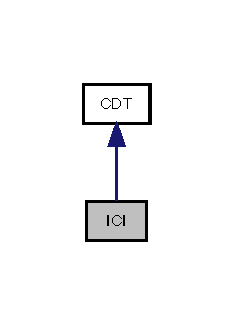
\includegraphics[width=112pt]{class_i_c_i__inherit__graph}
\end{center}
\end{figure}


Collaboration diagram for I\+CI\+:
\nopagebreak
\begin{figure}[H]
\begin{center}
\leavevmode
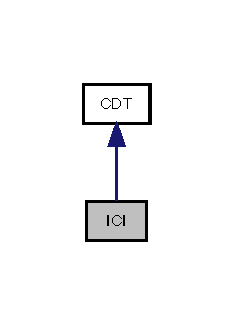
\includegraphics[width=112pt]{class_i_c_i__coll__graph}
\end{center}
\end{figure}
\subsection*{Public Member Functions}
\begin{DoxyCompactItemize}
\item 
\mbox{\hyperlink{class_i_c_i_a66a75673204429732da8b21435a625d4}{I\+CI}} (int S0, int nu, double gamma)
\begin{DoxyCompactList}\small\item\em Constructor of \mbox{\hyperlink{class_i_c_i}{I\+CI}}, i.\+e. the \mbox{\hyperlink{class_i_c_i}{I\+CI}} change detection procedure. \end{DoxyCompactList}\item 
\mbox{\hyperlink{class_c_d_t___result}{C\+D\+T\+\_\+\+Result}} \mbox{\hyperlink{class_i_c_i_a6a26d0c0a207ddd1f474bbdd226d82c8}{run}} (double reward) override
\begin{DoxyCompactList}\small\item\em run the \mbox{\hyperlink{class_i_c_i}{I\+CI}} algorithm \end{DoxyCompactList}\item 
void \mbox{\hyperlink{class_i_c_i_a24fe71d12a6dcb070cb87c342874fd33}{reset}} () override
\begin{DoxyCompactList}\small\item\em reset the \mbox{\hyperlink{class_i_c_i}{I\+CI}} algorithm \end{DoxyCompactList}\end{DoxyCompactItemize}


\subsection{Detailed Description}
\mbox{\hyperlink{class_c_d_t}{C\+DT}} with the \mbox{\hyperlink{class_i_c_i}{I\+CI}} algorithm. 

\subsection{Constructor \& Destructor Documentation}
\mbox{\Hypertarget{class_i_c_i_a66a75673204429732da8b21435a625d4}\label{class_i_c_i_a66a75673204429732da8b21435a625d4}} 
\index{I\+CI@{I\+CI}!I\+CI@{I\+CI}}
\index{I\+CI@{I\+CI}!I\+CI@{I\+CI}}
\subsubsection{\texorpdfstring{I\+C\+I()}{ICI()}}
{\footnotesize\ttfamily I\+C\+I\+::\+I\+CI (\begin{DoxyParamCaption}\item[{int}]{S0,  }\item[{int}]{nu,  }\item[{double}]{gamma }\end{DoxyParamCaption})}



Constructor of \mbox{\hyperlink{class_i_c_i}{I\+CI}}, i.\+e. the \mbox{\hyperlink{class_i_c_i}{I\+CI}} change detection procedure. 


\begin{DoxyParams}{Parameters}
{\em S0} & integer, number of initialization batches \\
\hline
{\em nu} & integer, length of each batch \\
\hline
{\em gamma} & double, confidence parameters used for the confidence intervals \\
\hline
\end{DoxyParams}


\subsection{Member Function Documentation}
\mbox{\Hypertarget{class_i_c_i_a24fe71d12a6dcb070cb87c342874fd33}\label{class_i_c_i_a24fe71d12a6dcb070cb87c342874fd33}} 
\index{I\+CI@{I\+CI}!reset@{reset}}
\index{reset@{reset}!I\+CI@{I\+CI}}
\subsubsection{\texorpdfstring{reset()}{reset()}}
{\footnotesize\ttfamily void I\+C\+I\+::reset (\begin{DoxyParamCaption}{ }\end{DoxyParamCaption})\hspace{0.3cm}{\ttfamily [override]}, {\ttfamily [virtual]}}



reset the \mbox{\hyperlink{class_i_c_i}{I\+CI}} algorithm 



Implements \mbox{\hyperlink{class_c_d_t_a46446ec219a819466ff418d9ab7aa728}{C\+DT}}.

\mbox{\Hypertarget{class_i_c_i_a6a26d0c0a207ddd1f474bbdd226d82c8}\label{class_i_c_i_a6a26d0c0a207ddd1f474bbdd226d82c8}} 
\index{I\+CI@{I\+CI}!run@{run}}
\index{run@{run}!I\+CI@{I\+CI}}
\subsubsection{\texorpdfstring{run()}{run()}}
{\footnotesize\ttfamily \mbox{\hyperlink{class_c_d_t___result}{C\+D\+T\+\_\+\+Result}} I\+C\+I\+::run (\begin{DoxyParamCaption}\item[{double}]{reward }\end{DoxyParamCaption})\hspace{0.3cm}{\ttfamily [override]}, {\ttfamily [virtual]}}



run the \mbox{\hyperlink{class_i_c_i}{I\+CI}} algorithm 


\begin{DoxyParams}{Parameters}
{\em reward} & double, the new datum that must be analysed by the \mbox{\hyperlink{class_c_d_t}{C\+DT}} \\
\hline
\end{DoxyParams}
\begin{DoxyReturn}{Returns}
a \mbox{\hyperlink{class_c_d_t___result}{C\+D\+T\+\_\+\+Result}} that contains the alarm and the estimated timestep change (this second part is not implemented!) 
\end{DoxyReturn}


Implements \mbox{\hyperlink{class_c_d_t_a2493aeb166403f448ec689d2f7b85dbc}{C\+DT}}.



The documentation for this class was generated from the following files\+:\begin{DoxyCompactItemize}
\item 
src/\mbox{\hyperlink{cdt_8h}{cdt.\+h}}\item 
src/\mbox{\hyperlink{cdt_8cpp}{cdt.\+cpp}}\end{DoxyCompactItemize}

\hypertarget{class_input_parser}{}\section{Input\+Parser Class Reference}
\label{class_input_parser}\index{Input\+Parser@{Input\+Parser}}


class whose goal is to parse the input arguments of the program  




{\ttfamily \#include $<$input\+\_\+parser.\+h$>$}

\subsection*{Public Member Functions}
\begin{DoxyCompactItemize}
\item 
\mbox{\hyperlink{class_input_parser_af9fa5ead1f28b5294a713410df5b9531}{Input\+Parser}} (int \&argc, char $\ast$$\ast$argv)
\begin{DoxyCompactList}\small\item\em constructor of \mbox{\hyperlink{class_input_parser}{Input\+Parser}} \end{DoxyCompactList}\item 
const string \& \mbox{\hyperlink{class_input_parser_a494c1de8c06fbb5a88343686e36fbf50}{get\+Cmd\+Option}} (const string \&option) const
\begin{DoxyCompactList}\small\item\em returns the string in argv after the specified option \end{DoxyCompactList}\item 
bool \mbox{\hyperlink{class_input_parser_ad3d06a9c59e91f425295bdc8408e0544}{cmd\+Option\+Exists}} (const string \&option) const
\begin{DoxyCompactList}\small\item\em returns true if the specified option exists in ergv. Return false otherwise \end{DoxyCompactList}\end{DoxyCompactItemize}


\subsection{Detailed Description}
class whose goal is to parse the input arguments of the program 

\begin{DoxyAuthor}{Author}
iain (stackoverflow) 
\end{DoxyAuthor}


\subsection{Constructor \& Destructor Documentation}
\mbox{\Hypertarget{class_input_parser_af9fa5ead1f28b5294a713410df5b9531}\label{class_input_parser_af9fa5ead1f28b5294a713410df5b9531}} 
\index{Input\+Parser@{Input\+Parser}!Input\+Parser@{Input\+Parser}}
\index{Input\+Parser@{Input\+Parser}!Input\+Parser@{Input\+Parser}}
\subsubsection{\texorpdfstring{Input\+Parser()}{InputParser()}}
{\footnotesize\ttfamily Input\+Parser\+::\+Input\+Parser (\begin{DoxyParamCaption}\item[{int \&}]{argc,  }\item[{char $\ast$$\ast$}]{argv }\end{DoxyParamCaption})}



constructor of \mbox{\hyperlink{class_input_parser}{Input\+Parser}} 


\begin{DoxyParams}{Parameters}
{\em argc} & the argc of the main \\
\hline
{\em argv} & the argv of the main \\
\hline
\end{DoxyParams}


\subsection{Member Function Documentation}
\mbox{\Hypertarget{class_input_parser_ad3d06a9c59e91f425295bdc8408e0544}\label{class_input_parser_ad3d06a9c59e91f425295bdc8408e0544}} 
\index{Input\+Parser@{Input\+Parser}!cmd\+Option\+Exists@{cmd\+Option\+Exists}}
\index{cmd\+Option\+Exists@{cmd\+Option\+Exists}!Input\+Parser@{Input\+Parser}}
\subsubsection{\texorpdfstring{cmd\+Option\+Exists()}{cmdOptionExists()}}
{\footnotesize\ttfamily bool Input\+Parser\+::cmd\+Option\+Exists (\begin{DoxyParamCaption}\item[{const string \&}]{option }\end{DoxyParamCaption}) const}



returns true if the specified option exists in ergv. Return false otherwise 


\begin{DoxyParams}{Parameters}
{\em option} & string, the option to check \\
\hline
\end{DoxyParams}
\begin{DoxyReturn}{Returns}
a boolean representing the presence of the specified option in argv
\end{DoxyReturn}
\begin{DoxyAuthor}{Author}
iain 
\end{DoxyAuthor}
\mbox{\Hypertarget{class_input_parser_a494c1de8c06fbb5a88343686e36fbf50}\label{class_input_parser_a494c1de8c06fbb5a88343686e36fbf50}} 
\index{Input\+Parser@{Input\+Parser}!get\+Cmd\+Option@{get\+Cmd\+Option}}
\index{get\+Cmd\+Option@{get\+Cmd\+Option}!Input\+Parser@{Input\+Parser}}
\subsubsection{\texorpdfstring{get\+Cmd\+Option()}{getCmdOption()}}
{\footnotesize\ttfamily const string \& Input\+Parser\+::get\+Cmd\+Option (\begin{DoxyParamCaption}\item[{const string \&}]{option }\end{DoxyParamCaption}) const}



returns the string in argv after the specified option 


\begin{DoxyParams}{Parameters}
{\em option} & string, the option to check (e.\+g. -\/d) \\
\hline
\end{DoxyParams}
\begin{DoxyReturn}{Returns}
the string after the specified option
\end{DoxyReturn}
\begin{DoxyAuthor}{Author}
iain 
\end{DoxyAuthor}


The documentation for this class was generated from the following files\+:\begin{DoxyCompactItemize}
\item 
src/\mbox{\hyperlink{input__parser_8h}{input\+\_\+parser.\+h}}\item 
src/\mbox{\hyperlink{input__parser_8cpp}{input\+\_\+parser.\+cpp}}\end{DoxyCompactItemize}

\hypertarget{class_m_a_b}{}\section{M\+AB Class Reference}
\label{class_m_a_b}\index{M\+AB@{M\+AB}}


Class representing a \mbox{\hyperlink{class_m_a_b}{M\+AB}} setting, which is a collection of arms.  




{\ttfamily \#include $<$mab.\+h$>$}



Inheritance diagram for M\+AB\+:
\nopagebreak
\begin{figure}[H]
\begin{center}
\leavevmode
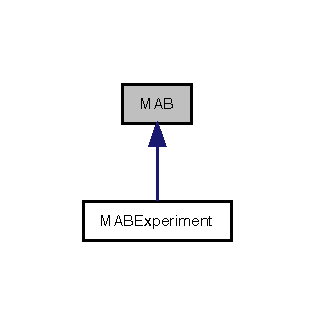
\includegraphics[width=151pt]{class_m_a_b__inherit__graph}
\end{center}
\end{figure}
\subsection*{Public Member Functions}
\begin{DoxyCompactItemize}
\item 
virtual vector$<$ int $>$ \mbox{\hyperlink{class_m_a_b_a8323d26ac3720c2f3949298d5f7cf60f}{get\+\_\+available\+\_\+actions}} ()=0
\item 
virtual double \mbox{\hyperlink{class_m_a_b_a83c6ba499e761ea4a246aa7bb790eb46}{observe\+\_\+reward}} (int action)=0
\end{DoxyCompactItemize}


\subsection{Detailed Description}
Class representing a \mbox{\hyperlink{class_m_a_b}{M\+AB}} setting, which is a collection of arms. 

\subsection{Member Function Documentation}
\mbox{\Hypertarget{class_m_a_b_a8323d26ac3720c2f3949298d5f7cf60f}\label{class_m_a_b_a8323d26ac3720c2f3949298d5f7cf60f}} 
\index{M\+AB@{M\+AB}!get\+\_\+available\+\_\+actions@{get\+\_\+available\+\_\+actions}}
\index{get\+\_\+available\+\_\+actions@{get\+\_\+available\+\_\+actions}!M\+AB@{M\+AB}}
\subsubsection{\texorpdfstring{get\+\_\+available\+\_\+actions()}{get\_available\_actions()}}
{\footnotesize\ttfamily virtual vector$<$int$>$ M\+A\+B\+::get\+\_\+available\+\_\+actions (\begin{DoxyParamCaption}{ }\end{DoxyParamCaption})\hspace{0.3cm}{\ttfamily [pure virtual]}}

\begin{DoxyReturn}{Returns}
a vector containing the ids of all the currently available actions 
\end{DoxyReturn}


Implemented in \mbox{\hyperlink{class_m_a_b_experiment_af64386f9138dcd31873d9218b7adf6fb}{M\+A\+B\+Experiment}}.

\mbox{\Hypertarget{class_m_a_b_a83c6ba499e761ea4a246aa7bb790eb46}\label{class_m_a_b_a83c6ba499e761ea4a246aa7bb790eb46}} 
\index{M\+AB@{M\+AB}!observe\+\_\+reward@{observe\+\_\+reward}}
\index{observe\+\_\+reward@{observe\+\_\+reward}!M\+AB@{M\+AB}}
\subsubsection{\texorpdfstring{observe\+\_\+reward()}{observe\_reward()}}
{\footnotesize\ttfamily virtual double M\+A\+B\+::observe\+\_\+reward (\begin{DoxyParamCaption}\item[{int}]{action }\end{DoxyParamCaption})\hspace{0.3cm}{\ttfamily [pure virtual]}}


\begin{DoxyParams}{Parameters}
{\em action} & integer, the arm to pull \\
\hline
\end{DoxyParams}
\begin{DoxyReturn}{Returns}
the reward obtained pulling the specified arm 
\end{DoxyReturn}


Implemented in \mbox{\hyperlink{class_m_a_b_experiment_acf2ca557df3d30325d8ff180c223a54a}{M\+A\+B\+Experiment}}.



The documentation for this class was generated from the following file\+:\begin{DoxyCompactItemize}
\item 
src/\mbox{\hyperlink{mab_8h}{mab.\+h}}\end{DoxyCompactItemize}

\hypertarget{class_m_a_b_algorithm}{}\section{M\+A\+B\+Algorithm Class Reference}
\label{class_m_a_b_algorithm}\index{M\+A\+B\+Algorithm@{M\+A\+B\+Algorithm}}


Base class of all the algorithms for multi armed bandits.  




{\ttfamily \#include $<$mabalg.\+h$>$}



Inheritance diagram for M\+A\+B\+Algorithm\+:
\nopagebreak
\begin{figure}[H]
\begin{center}
\leavevmode
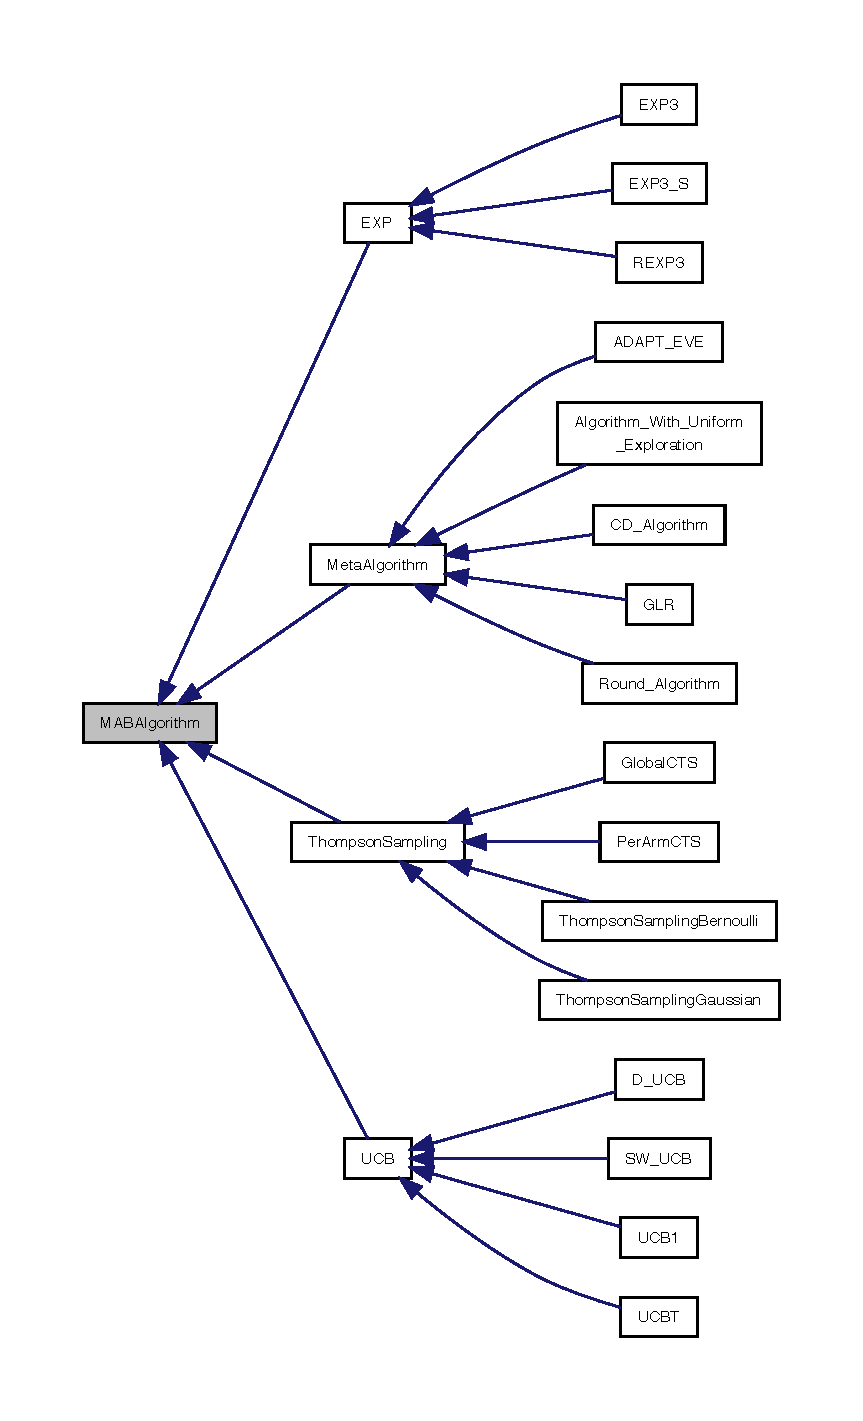
\includegraphics[height=550pt]{class_m_a_b_algorithm__inherit__graph}
\end{center}
\end{figure}
\subsection*{Public Member Functions}
\begin{DoxyCompactItemize}
\item 
\mbox{\hyperlink{class_m_a_b_algorithm_a9a938041685a1912995d427027971de4}{M\+A\+B\+Algorithm}} (string \mbox{\hyperlink{class_m_a_b_algorithm_a77b10ecc4b49d519c557f65358167b82}{name}}, int \mbox{\hyperlink{class_m_a_b_algorithm_a340fa9e83e85b092f2c6125fc4e8549b}{num\+\_\+of\+\_\+arms}})
\item 
virtual int \mbox{\hyperlink{class_m_a_b_algorithm_afb48f01df0e1860d19759f6e20335007}{choose\+\_\+action}} ()=0
\item 
virtual void \mbox{\hyperlink{class_m_a_b_algorithm_aa584b3d6b86fa050e3389be9781b5782}{receive\+\_\+reward}} (double reward, int pulled\+\_\+arm)
\begin{DoxyCompactList}\small\item\em Update the internal variables of the algorithm according to the new received reward. \end{DoxyCompactList}\item 
virtual void \mbox{\hyperlink{class_m_a_b_algorithm_ad5761cee0b0e3421d1f043dbcc0b5f85}{reset}} (int action=-\/1)
\begin{DoxyCompactList}\small\item\em resets the internal variables of the algorithm \end{DoxyCompactList}\end{DoxyCompactItemize}
\subsection*{Public Attributes}
\begin{DoxyCompactItemize}
\item 
vector$<$ int $>$ \mbox{\hyperlink{class_m_a_b_algorithm_a46daff3833924ea5ebbda86113699fd3}{num\+\_\+of\+\_\+pulls}}
\item 
string \mbox{\hyperlink{class_m_a_b_algorithm_a77b10ecc4b49d519c557f65358167b82}{name}}
\end{DoxyCompactItemize}
\subsection*{Protected Attributes}
\begin{DoxyCompactItemize}
\item 
int \mbox{\hyperlink{class_m_a_b_algorithm_a340fa9e83e85b092f2c6125fc4e8549b}{num\+\_\+of\+\_\+arms}} = 0
\end{DoxyCompactItemize}


\subsection{Detailed Description}
Base class of all the algorithms for multi armed bandits. 

\subsection{Constructor \& Destructor Documentation}
\mbox{\Hypertarget{class_m_a_b_algorithm_a9a938041685a1912995d427027971de4}\label{class_m_a_b_algorithm_a9a938041685a1912995d427027971de4}} 
\index{M\+A\+B\+Algorithm@{M\+A\+B\+Algorithm}!M\+A\+B\+Algorithm@{M\+A\+B\+Algorithm}}
\index{M\+A\+B\+Algorithm@{M\+A\+B\+Algorithm}!M\+A\+B\+Algorithm@{M\+A\+B\+Algorithm}}
\subsubsection{\texorpdfstring{M\+A\+B\+Algorithm()}{MABAlgorithm()}}
{\footnotesize\ttfamily M\+A\+B\+Algorithm\+::\+M\+A\+B\+Algorithm (\begin{DoxyParamCaption}\item[{string}]{name,  }\item[{int}]{num\+\_\+of\+\_\+arms }\end{DoxyParamCaption})}


\begin{DoxyParams}{Parameters}
{\em name} & string, id of the algorithm \\
\hline
{\em num\+\_\+of\+\_\+arms} & integer, number of arms the algorithm will work with \\
\hline
\end{DoxyParams}


\subsection{Member Function Documentation}
\mbox{\Hypertarget{class_m_a_b_algorithm_afb48f01df0e1860d19759f6e20335007}\label{class_m_a_b_algorithm_afb48f01df0e1860d19759f6e20335007}} 
\index{M\+A\+B\+Algorithm@{M\+A\+B\+Algorithm}!choose\+\_\+action@{choose\+\_\+action}}
\index{choose\+\_\+action@{choose\+\_\+action}!M\+A\+B\+Algorithm@{M\+A\+B\+Algorithm}}
\subsubsection{\texorpdfstring{choose\+\_\+action()}{choose\_action()}}
{\footnotesize\ttfamily virtual int M\+A\+B\+Algorithm\+::choose\+\_\+action (\begin{DoxyParamCaption}{ }\end{DoxyParamCaption})\hspace{0.3cm}{\ttfamily [pure virtual]}}

\mbox{[}choose\+\_\+action description\mbox{]} \begin{DoxyReturn}{Returns}
\mbox{[}description\mbox{]} 

an integer representing the chosen arm 
\end{DoxyReturn}


Implemented in \mbox{\hyperlink{class_g_l_r_ad6b3e9f19e0bea4d6067b491c33640e0}{G\+LR}}, \mbox{\hyperlink{class_a_d_a_p_t___e_v_e_aa878cacd23fbe8743493623f8a9be6d6}{A\+D\+A\+P\+T\+\_\+\+E\+VE}}, \mbox{\hyperlink{class_per_arm_c_t_s_ab8904bef227b13aed75aade589421c5a}{Per\+Arm\+C\+TS}}, \mbox{\hyperlink{class_s_w___u_c_b_a819ec3b60cd7a8e5f3983b979d3d765f}{S\+W\+\_\+\+U\+CB}}, \mbox{\hyperlink{class_c_d___algorithm_a10d80cbf4687e2c0ef69466ee6deb1a9}{C\+D\+\_\+\+Algorithm}}, \mbox{\hyperlink{class_r_e_x_p3_aba9cbcdc74602157701b022a7758d584}{R\+E\+X\+P3}}, \mbox{\hyperlink{class_global_c_t_s_a48f9873be9f993e78fdbdd93ad4806bc}{Global\+C\+TS}}, \mbox{\hyperlink{class_d___u_c_b_ac48b99c21eb02361707988f6ac012408}{D\+\_\+\+U\+CB}}, \mbox{\hyperlink{class_algorithm___with___uniform___exploration_a42d5f75def328c83dce00f73dbe26d58}{Algorithm\+\_\+\+With\+\_\+\+Uniform\+\_\+\+Exploration}}, \mbox{\hyperlink{class_e_x_p3___s_afc9e4825004f5f541f774ac0debe6bee}{E\+X\+P3\+\_\+S}}, \mbox{\hyperlink{class_thompson_sampling_gaussian_a36e15e9a5d9f5cae94fef686c2cbb4be}{Thompson\+Sampling\+Gaussian}}, \mbox{\hyperlink{class_u_c_b_t_a6bebf23b2dd926e49794a4fb0fefe358}{U\+C\+BT}}, \mbox{\hyperlink{class_round___algorithm_a019a9a7a564a49512f5089c3829e6f4e}{Round\+\_\+\+Algorithm}}, \mbox{\hyperlink{class_e_x_p3_adb52fc51fbc5ef97e3d67c2437634be8}{E\+X\+P3}}, \mbox{\hyperlink{class_thompson_sampling_bernoulli_a80f2f22f0bbf71b60a7a7133ce49d917}{Thompson\+Sampling\+Bernoulli}}, and \mbox{\hyperlink{class_u_c_b1_ac71b279c529fdcca156e984550ad3ed3}{U\+C\+B1}}.

\mbox{\Hypertarget{class_m_a_b_algorithm_aa584b3d6b86fa050e3389be9781b5782}\label{class_m_a_b_algorithm_aa584b3d6b86fa050e3389be9781b5782}} 
\index{M\+A\+B\+Algorithm@{M\+A\+B\+Algorithm}!receive\+\_\+reward@{receive\+\_\+reward}}
\index{receive\+\_\+reward@{receive\+\_\+reward}!M\+A\+B\+Algorithm@{M\+A\+B\+Algorithm}}
\subsubsection{\texorpdfstring{receive\+\_\+reward()}{receive\_reward()}}
{\footnotesize\ttfamily void M\+A\+B\+Algorithm\+::receive\+\_\+reward (\begin{DoxyParamCaption}\item[{double}]{reward,  }\item[{int}]{pulled\+\_\+arm }\end{DoxyParamCaption})\hspace{0.3cm}{\ttfamily [virtual]}}



Update the internal variables of the algorithm according to the new received reward. 


\begin{DoxyParams}{Parameters}
{\em reward} & double, new received reward \\
\hline
{\em pulled\+\_\+arm} & integer, represents the pulled arm \\
\hline
\end{DoxyParams}


Reimplemented in \mbox{\hyperlink{class_g_l_r_ad8e409518a110bd57f42a2de1b759707}{G\+LR}}, \mbox{\hyperlink{class_a_d_a_p_t___e_v_e_ab626b3d8e8f27200e35a0fc3c80f9539}{A\+D\+A\+P\+T\+\_\+\+E\+VE}}, \mbox{\hyperlink{class_per_arm_c_t_s_af9ac7b45d329223ce506e977b96a32ee}{Per\+Arm\+C\+TS}}, \mbox{\hyperlink{class_s_w___u_c_b_acddb0c5385d33d332a2fbf1b739142c2}{S\+W\+\_\+\+U\+CB}}, \mbox{\hyperlink{class_c_d___algorithm_a2427ddf68550eda00a0992b875c10834}{C\+D\+\_\+\+Algorithm}}, \mbox{\hyperlink{class_r_e_x_p3_a535d6667ecfa71568a68a5a09c44d4bf}{R\+E\+X\+P3}}, \mbox{\hyperlink{class_global_c_t_s_acb2f35fa8c6b2ae61912f6f337ed815f}{Global\+C\+TS}}, \mbox{\hyperlink{class_d___u_c_b_a23b79f3f23095ae6e824b36a3856ff7c}{D\+\_\+\+U\+CB}}, \mbox{\hyperlink{class_algorithm___with___uniform___exploration_a946808f681cd7b54bd557e1d8f15c5d0}{Algorithm\+\_\+\+With\+\_\+\+Uniform\+\_\+\+Exploration}}, \mbox{\hyperlink{class_e_x_p3___s_a93cef92a4f0213f7d247768b610071ad}{E\+X\+P3\+\_\+S}}, \mbox{\hyperlink{class_thompson_sampling_gaussian_a21d02f760e6738a8e209f46e57ffa341}{Thompson\+Sampling\+Gaussian}}, \mbox{\hyperlink{class_u_c_b_t_a0e9b24c391f3934e59809419e0b04e52}{U\+C\+BT}}, \mbox{\hyperlink{class_round___algorithm_a945da188a51c00d1923f4eb8434042eb}{Round\+\_\+\+Algorithm}}, \mbox{\hyperlink{class_e_x_p3_a9408f963aa533ffb298deba2fbc65529}{E\+X\+P3}}, \mbox{\hyperlink{class_thompson_sampling_bernoulli_a02d2aabd642f0b1149963539178f2a1e}{Thompson\+Sampling\+Bernoulli}}, and \mbox{\hyperlink{class_u_c_b1_a79106e98a38550c3f1f03e10f72226c6}{U\+C\+B1}}.

\mbox{\Hypertarget{class_m_a_b_algorithm_ad5761cee0b0e3421d1f043dbcc0b5f85}\label{class_m_a_b_algorithm_ad5761cee0b0e3421d1f043dbcc0b5f85}} 
\index{M\+A\+B\+Algorithm@{M\+A\+B\+Algorithm}!reset@{reset}}
\index{reset@{reset}!M\+A\+B\+Algorithm@{M\+A\+B\+Algorithm}}
\subsubsection{\texorpdfstring{reset()}{reset()}}
{\footnotesize\ttfamily void M\+A\+B\+Algorithm\+::reset (\begin{DoxyParamCaption}\item[{int}]{action = {\ttfamily -\/1} }\end{DoxyParamCaption})\hspace{0.3cm}{\ttfamily [virtual]}}



resets the internal variables of the algorithm 


\begin{DoxyParams}{Parameters}
{\em action} & integer, specifies which variables to reset. If in (0, num\+\_\+of\+\_\+arms -\/ 1), then it resets only the info related to such arm. If == -\/1, resets all the arms. \\
\hline
\end{DoxyParams}


Reimplemented in \mbox{\hyperlink{class_g_l_r_ad6c979e855b56e80ecfc54c8c93f035e}{G\+LR}}, \mbox{\hyperlink{class_a_d_a_p_t___e_v_e_aa89f094cbcba01accada672f0924a5f3}{A\+D\+A\+P\+T\+\_\+\+E\+VE}}, \mbox{\hyperlink{class_per_arm_c_t_s_ae5f8998bfb68b4a9cbdea7bca34f5cbe}{Per\+Arm\+C\+TS}}, \mbox{\hyperlink{class_s_w___u_c_b_afbbe9a17cc00402d2487260b530bbee2}{S\+W\+\_\+\+U\+CB}}, \mbox{\hyperlink{class_c_d___algorithm_a493e6eaafb4ab105c94e9e4c33143d39}{C\+D\+\_\+\+Algorithm}}, \mbox{\hyperlink{class_r_e_x_p3_ad99a97c07f75addc64e612774de81307}{R\+E\+X\+P3}}, \mbox{\hyperlink{class_global_c_t_s_a1e2c899b85ec7adf92a28ac758f556b5}{Global\+C\+TS}}, \mbox{\hyperlink{class_d___u_c_b_a454ffcd1e17989f0b049790cfc5fc515}{D\+\_\+\+U\+CB}}, \mbox{\hyperlink{class_algorithm___with___uniform___exploration_a96b0df2a59099ba8b4cc83f21b407642}{Algorithm\+\_\+\+With\+\_\+\+Uniform\+\_\+\+Exploration}}, \mbox{\hyperlink{class_e_x_p3___s_a70bfd4fc19a73ab7d2903672c36b2765}{E\+X\+P3\+\_\+S}}, \mbox{\hyperlink{class_thompson_sampling_gaussian_a847a421af9da4c81c10c395ebde1d8c8}{Thompson\+Sampling\+Gaussian}}, \mbox{\hyperlink{class_u_c_b_t_a4830934c071870d6f8680f90a247f9a7}{U\+C\+BT}}, \mbox{\hyperlink{class_round___algorithm_ae2c21984dbd89f5ba1a4f530472cf7f7}{Round\+\_\+\+Algorithm}}, \mbox{\hyperlink{class_e_x_p3_a30530aa50cd991eda2f9f2f170b92d0e}{E\+X\+P3}}, \mbox{\hyperlink{class_thompson_sampling_bernoulli_abb2e2c252333090ac1bd63e4297e99ba}{Thompson\+Sampling\+Bernoulli}}, and \mbox{\hyperlink{class_u_c_b1_aa426545f69a7e168ffcdcc3c9e8cd490}{U\+C\+B1}}.



\subsection{Member Data Documentation}
\mbox{\Hypertarget{class_m_a_b_algorithm_a77b10ecc4b49d519c557f65358167b82}\label{class_m_a_b_algorithm_a77b10ecc4b49d519c557f65358167b82}} 
\index{M\+A\+B\+Algorithm@{M\+A\+B\+Algorithm}!name@{name}}
\index{name@{name}!M\+A\+B\+Algorithm@{M\+A\+B\+Algorithm}}
\subsubsection{\texorpdfstring{name}{name}}
{\footnotesize\ttfamily string M\+A\+B\+Algorithm\+::name}

\mbox{\Hypertarget{class_m_a_b_algorithm_a340fa9e83e85b092f2c6125fc4e8549b}\label{class_m_a_b_algorithm_a340fa9e83e85b092f2c6125fc4e8549b}} 
\index{M\+A\+B\+Algorithm@{M\+A\+B\+Algorithm}!num\+\_\+of\+\_\+arms@{num\+\_\+of\+\_\+arms}}
\index{num\+\_\+of\+\_\+arms@{num\+\_\+of\+\_\+arms}!M\+A\+B\+Algorithm@{M\+A\+B\+Algorithm}}
\subsubsection{\texorpdfstring{num\+\_\+of\+\_\+arms}{num\_of\_arms}}
{\footnotesize\ttfamily int M\+A\+B\+Algorithm\+::num\+\_\+of\+\_\+arms = 0\hspace{0.3cm}{\ttfamily [protected]}}

\mbox{\Hypertarget{class_m_a_b_algorithm_a46daff3833924ea5ebbda86113699fd3}\label{class_m_a_b_algorithm_a46daff3833924ea5ebbda86113699fd3}} 
\index{M\+A\+B\+Algorithm@{M\+A\+B\+Algorithm}!num\+\_\+of\+\_\+pulls@{num\+\_\+of\+\_\+pulls}}
\index{num\+\_\+of\+\_\+pulls@{num\+\_\+of\+\_\+pulls}!M\+A\+B\+Algorithm@{M\+A\+B\+Algorithm}}
\subsubsection{\texorpdfstring{num\+\_\+of\+\_\+pulls}{num\_of\_pulls}}
{\footnotesize\ttfamily vector$<$int$>$ M\+A\+B\+Algorithm\+::num\+\_\+of\+\_\+pulls}



The documentation for this class was generated from the following files\+:\begin{DoxyCompactItemize}
\item 
src/\mbox{\hyperlink{mabalg_8h}{mabalg.\+h}}\item 
src/\mbox{\hyperlink{mabalg_8cpp}{mabalg.\+cpp}}\end{DoxyCompactItemize}

\hypertarget{class_m_a_b_experiment}{}\section{M\+A\+B\+Experiment Class Reference}
\label{class_m_a_b_experiment}\index{M\+A\+B\+Experiment@{M\+A\+B\+Experiment}}


In order to test different algorithms with the same data, they must be able to obtain the same reward when pulling an arm in the same timestep. The \mbox{\hyperlink{class_m_a_b_experiment}{M\+A\+B\+Experiment}} class generate all the rewards of the arms up to the time horizon, before the algorithm starts.  




{\ttfamily \#include $<$mab.\+h$>$}



Inheritance diagram for M\+A\+B\+Experiment\+:
\nopagebreak
\begin{figure}[H]
\begin{center}
\leavevmode
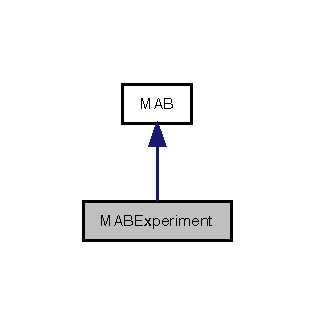
\includegraphics[width=151pt]{class_m_a_b_experiment__inherit__graph}
\end{center}
\end{figure}


Collaboration diagram for M\+A\+B\+Experiment\+:
\nopagebreak
\begin{figure}[H]
\begin{center}
\leavevmode
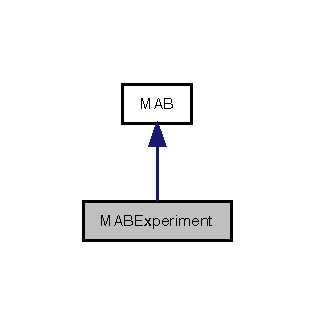
\includegraphics[width=151pt]{class_m_a_b_experiment__coll__graph}
\end{center}
\end{figure}
\subsection*{Public Member Functions}
\begin{DoxyCompactItemize}
\item 
\mbox{\hyperlink{class_m_a_b_experiment_a1f24b5ccad7521d47a7f4c3961867063}{M\+A\+B\+Experiment}} (vector$<$ \mbox{\hyperlink{class_distribution}{Distribution}} $\ast$$>$ \&\mbox{\hyperlink{class_m_a_b_experiment_abcea657cec661467e38422059dbd4a2d}{arms}})
\item 
vector$<$ vector$<$ double $>$ $>$ \mbox{\hyperlink{class_m_a_b_experiment_af31d09524129608838d5262678e8de18}{generate\+\_\+pulls}} (int timesteps)
\begin{DoxyCompactList}\small\item\em Generate the pulls for each arm up to the specified time horizon. \end{DoxyCompactList}\item 
vector$<$ int $>$ \mbox{\hyperlink{class_m_a_b_experiment_af64386f9138dcd31873d9218b7adf6fb}{get\+\_\+available\+\_\+actions}} () override
\item 
double \mbox{\hyperlink{class_m_a_b_experiment_acf2ca557df3d30325d8ff180c223a54a}{observe\+\_\+reward}} (int action) override
\item 
void \mbox{\hyperlink{class_m_a_b_experiment_a0159e6c16372d282c0e2afd711da22c8}{next\+\_\+step}} ()
\begin{DoxyCompactList}\small\item\em advance the time tick by one. This must be done after allt he algorithms have pulled the arm in order to advance to the next timestep. \end{DoxyCompactList}\item 
void \mbox{\hyperlink{class_m_a_b_experiment_a8fda8c3d5f6b58751243d59b86cc4f07}{reset}} ()
\begin{DoxyCompactList}\small\item\em Reset the current timestep and the generated pulls. \end{DoxyCompactList}\end{DoxyCompactItemize}
\subsection*{Public Attributes}
\begin{DoxyCompactItemize}
\item 
vector$<$ \mbox{\hyperlink{class_distribution}{Distribution}} $\ast$ $>$ \mbox{\hyperlink{class_m_a_b_experiment_abcea657cec661467e38422059dbd4a2d}{arms}}
\end{DoxyCompactItemize}


\subsection{Detailed Description}
In order to test different algorithms with the same data, they must be able to obtain the same reward when pulling an arm in the same timestep. The \mbox{\hyperlink{class_m_a_b_experiment}{M\+A\+B\+Experiment}} class generate all the rewards of the arms up to the time horizon, before the algorithm starts. 

\subsection{Constructor \& Destructor Documentation}
\mbox{\Hypertarget{class_m_a_b_experiment_a1f24b5ccad7521d47a7f4c3961867063}\label{class_m_a_b_experiment_a1f24b5ccad7521d47a7f4c3961867063}} 
\index{M\+A\+B\+Experiment@{M\+A\+B\+Experiment}!M\+A\+B\+Experiment@{M\+A\+B\+Experiment}}
\index{M\+A\+B\+Experiment@{M\+A\+B\+Experiment}!M\+A\+B\+Experiment@{M\+A\+B\+Experiment}}
\subsubsection{\texorpdfstring{M\+A\+B\+Experiment()}{MABExperiment()}}
{\footnotesize\ttfamily M\+A\+B\+Experiment\+::\+M\+A\+B\+Experiment (\begin{DoxyParamCaption}\item[{vector$<$ \mbox{\hyperlink{class_distribution}{Distribution}} $\ast$$>$ \&}]{arms }\end{DoxyParamCaption})}


\begin{DoxyParams}{Parameters}
{\em arms} & vector$<$\+Distribution$\ast$$>$\&, the vector of arms for this \mbox{\hyperlink{class_m_a_b}{M\+AB}} setting \\
\hline
\end{DoxyParams}


\subsection{Member Function Documentation}
\mbox{\Hypertarget{class_m_a_b_experiment_af31d09524129608838d5262678e8de18}\label{class_m_a_b_experiment_af31d09524129608838d5262678e8de18}} 
\index{M\+A\+B\+Experiment@{M\+A\+B\+Experiment}!generate\+\_\+pulls@{generate\+\_\+pulls}}
\index{generate\+\_\+pulls@{generate\+\_\+pulls}!M\+A\+B\+Experiment@{M\+A\+B\+Experiment}}
\subsubsection{\texorpdfstring{generate\+\_\+pulls()}{generate\_pulls()}}
{\footnotesize\ttfamily vector$<$ vector$<$ double $>$ $>$ M\+A\+B\+Experiment\+::generate\+\_\+pulls (\begin{DoxyParamCaption}\item[{int}]{timesteps }\end{DoxyParamCaption})}



Generate the pulls for each arm up to the specified time horizon. 


\begin{DoxyParams}{Parameters}
{\em timesteps} & integer, the time horizon \\
\hline
\end{DoxyParams}
\mbox{\Hypertarget{class_m_a_b_experiment_af64386f9138dcd31873d9218b7adf6fb}\label{class_m_a_b_experiment_af64386f9138dcd31873d9218b7adf6fb}} 
\index{M\+A\+B\+Experiment@{M\+A\+B\+Experiment}!get\+\_\+available\+\_\+actions@{get\+\_\+available\+\_\+actions}}
\index{get\+\_\+available\+\_\+actions@{get\+\_\+available\+\_\+actions}!M\+A\+B\+Experiment@{M\+A\+B\+Experiment}}
\subsubsection{\texorpdfstring{get\+\_\+available\+\_\+actions()}{get\_available\_actions()}}
{\footnotesize\ttfamily vector$<$ int $>$ M\+A\+B\+Experiment\+::get\+\_\+available\+\_\+actions (\begin{DoxyParamCaption}{ }\end{DoxyParamCaption})\hspace{0.3cm}{\ttfamily [override]}, {\ttfamily [virtual]}}

\begin{DoxyReturn}{Returns}
a vector containing the ids of all the currently available actions 
\end{DoxyReturn}


Implements \mbox{\hyperlink{class_m_a_b_a8323d26ac3720c2f3949298d5f7cf60f}{M\+AB}}.

\mbox{\Hypertarget{class_m_a_b_experiment_a0159e6c16372d282c0e2afd711da22c8}\label{class_m_a_b_experiment_a0159e6c16372d282c0e2afd711da22c8}} 
\index{M\+A\+B\+Experiment@{M\+A\+B\+Experiment}!next\+\_\+step@{next\+\_\+step}}
\index{next\+\_\+step@{next\+\_\+step}!M\+A\+B\+Experiment@{M\+A\+B\+Experiment}}
\subsubsection{\texorpdfstring{next\+\_\+step()}{next\_step()}}
{\footnotesize\ttfamily void M\+A\+B\+Experiment\+::next\+\_\+step (\begin{DoxyParamCaption}{ }\end{DoxyParamCaption})}



advance the time tick by one. This must be done after allt he algorithms have pulled the arm in order to advance to the next timestep. 

\mbox{\Hypertarget{class_m_a_b_experiment_acf2ca557df3d30325d8ff180c223a54a}\label{class_m_a_b_experiment_acf2ca557df3d30325d8ff180c223a54a}} 
\index{M\+A\+B\+Experiment@{M\+A\+B\+Experiment}!observe\+\_\+reward@{observe\+\_\+reward}}
\index{observe\+\_\+reward@{observe\+\_\+reward}!M\+A\+B\+Experiment@{M\+A\+B\+Experiment}}
\subsubsection{\texorpdfstring{observe\+\_\+reward()}{observe\_reward()}}
{\footnotesize\ttfamily double M\+A\+B\+Experiment\+::observe\+\_\+reward (\begin{DoxyParamCaption}\item[{int}]{action }\end{DoxyParamCaption})\hspace{0.3cm}{\ttfamily [override]}, {\ttfamily [virtual]}}


\begin{DoxyParams}{Parameters}
{\em action} & integer, the arm to pull \\
\hline
\end{DoxyParams}
\begin{DoxyReturn}{Returns}
the reward obtained pulling the specified arm 
\end{DoxyReturn}


Implements \mbox{\hyperlink{class_m_a_b_a83c6ba499e761ea4a246aa7bb790eb46}{M\+AB}}.

\mbox{\Hypertarget{class_m_a_b_experiment_a8fda8c3d5f6b58751243d59b86cc4f07}\label{class_m_a_b_experiment_a8fda8c3d5f6b58751243d59b86cc4f07}} 
\index{M\+A\+B\+Experiment@{M\+A\+B\+Experiment}!reset@{reset}}
\index{reset@{reset}!M\+A\+B\+Experiment@{M\+A\+B\+Experiment}}
\subsubsection{\texorpdfstring{reset()}{reset()}}
{\footnotesize\ttfamily void M\+A\+B\+Experiment\+::reset (\begin{DoxyParamCaption}{ }\end{DoxyParamCaption})}



Reset the current timestep and the generated pulls. 



\subsection{Member Data Documentation}
\mbox{\Hypertarget{class_m_a_b_experiment_abcea657cec661467e38422059dbd4a2d}\label{class_m_a_b_experiment_abcea657cec661467e38422059dbd4a2d}} 
\index{M\+A\+B\+Experiment@{M\+A\+B\+Experiment}!arms@{arms}}
\index{arms@{arms}!M\+A\+B\+Experiment@{M\+A\+B\+Experiment}}
\subsubsection{\texorpdfstring{arms}{arms}}
{\footnotesize\ttfamily vector$<$\mbox{\hyperlink{class_distribution}{Distribution}}$\ast$$>$ M\+A\+B\+Experiment\+::arms}



The documentation for this class was generated from the following files\+:\begin{DoxyCompactItemize}
\item 
src/\mbox{\hyperlink{mab_8h}{mab.\+h}}\item 
src/\mbox{\hyperlink{mab_8cpp}{mab.\+cpp}}\end{DoxyCompactItemize}

\hypertarget{class_meta_algorithm}{}\section{Meta\+Algorithm Class Reference}
\label{class_meta_algorithm}\index{Meta\+Algorithm@{Meta\+Algorithm}}


base class of all the meta-\/algorithms  




{\ttfamily \#include $<$meta\+\_\+algorithms.\+h$>$}



Inheritance diagram for Meta\+Algorithm\+:
\nopagebreak
\begin{figure}[H]
\begin{center}
\leavevmode
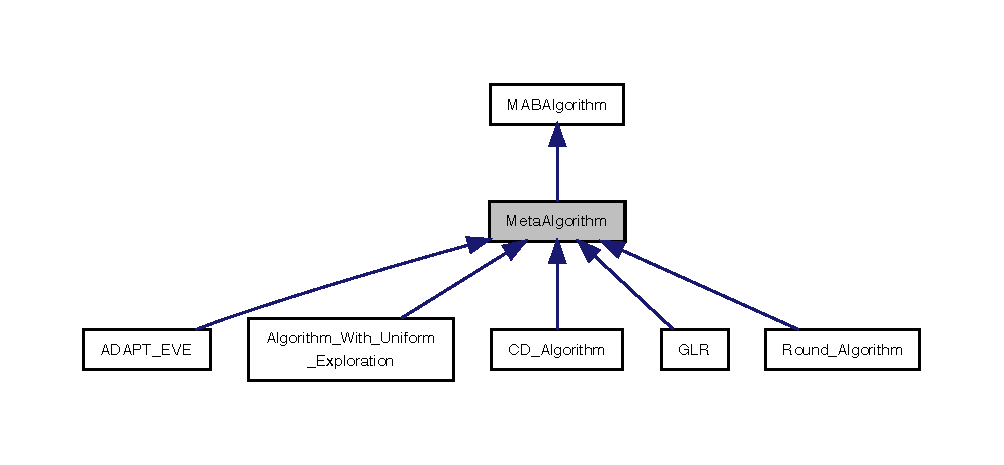
\includegraphics[width=350pt]{class_meta_algorithm__inherit__graph}
\end{center}
\end{figure}


Collaboration diagram for Meta\+Algorithm\+:
\nopagebreak
\begin{figure}[H]
\begin{center}
\leavevmode
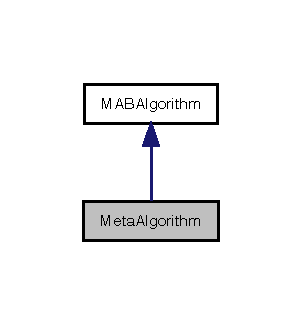
\includegraphics[width=145pt]{class_meta_algorithm__coll__graph}
\end{center}
\end{figure}
\subsection*{Public Member Functions}
\begin{DoxyCompactItemize}
\item 
\mbox{\hyperlink{class_meta_algorithm_a747f056c3483bf967b5cc69fef251cd0}{Meta\+Algorithm}} (string \mbox{\hyperlink{class_m_a_b_algorithm_a77b10ecc4b49d519c557f65358167b82}{name}}, int \mbox{\hyperlink{class_m_a_b_algorithm_a340fa9e83e85b092f2c6125fc4e8549b}{num\+\_\+of\+\_\+arms}})
\end{DoxyCompactItemize}
\subsection*{Additional Inherited Members}


\subsection{Detailed Description}
base class of all the meta-\/algorithms 

\subsection{Constructor \& Destructor Documentation}
\mbox{\Hypertarget{class_meta_algorithm_a747f056c3483bf967b5cc69fef251cd0}\label{class_meta_algorithm_a747f056c3483bf967b5cc69fef251cd0}} 
\index{Meta\+Algorithm@{Meta\+Algorithm}!Meta\+Algorithm@{Meta\+Algorithm}}
\index{Meta\+Algorithm@{Meta\+Algorithm}!Meta\+Algorithm@{Meta\+Algorithm}}
\subsubsection{\texorpdfstring{Meta\+Algorithm()}{MetaAlgorithm()}}
{\footnotesize\ttfamily Meta\+Algorithm\+::\+Meta\+Algorithm (\begin{DoxyParamCaption}\item[{string}]{name,  }\item[{int}]{num\+\_\+of\+\_\+arms }\end{DoxyParamCaption})}


\begin{DoxyParams}{Parameters}
{\em name} & string, id of the algorithm \\
\hline
{\em num\+\_\+of\+\_\+arms} & integer, number of arms the algorithm will work on \\
\hline
\end{DoxyParams}


The documentation for this class was generated from the following files\+:\begin{DoxyCompactItemize}
\item 
src/\mbox{\hyperlink{meta__algorithms_8h}{meta\+\_\+algorithms.\+h}}\item 
src/\mbox{\hyperlink{meta__algorithms_8cpp}{meta\+\_\+algorithms.\+cpp}}\end{DoxyCompactItemize}

\hypertarget{class_normal_distribution}{}\section{Normal\+Distribution Class Reference}
\label{class_normal_distribution}\index{Normal\+Distribution@{Normal\+Distribution}}


\mbox{\hyperlink{class_distribution}{Distribution}} of a normal distribution.  




{\ttfamily \#include $<$distribution.\+h$>$}



Inheritance diagram for Normal\+Distribution\+:
\nopagebreak
\begin{figure}[H]
\begin{center}
\leavevmode
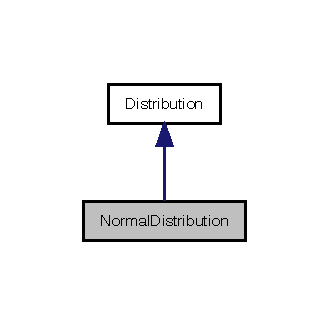
\includegraphics[width=158pt]{class_normal_distribution__inherit__graph}
\end{center}
\end{figure}


Collaboration diagram for Normal\+Distribution\+:
\nopagebreak
\begin{figure}[H]
\begin{center}
\leavevmode
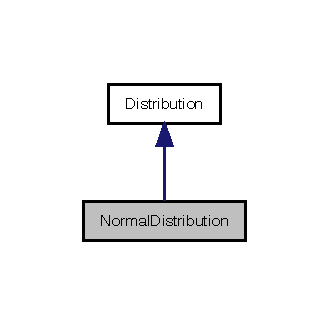
\includegraphics[width=158pt]{class_normal_distribution__coll__graph}
\end{center}
\end{figure}
\subsection*{Public Member Functions}
\begin{DoxyCompactItemize}
\item 
\mbox{\hyperlink{class_normal_distribution_a06673b1c5d2087cfa2461ba277ae6779}{Normal\+Distribution}} (string \mbox{\hyperlink{class_distribution_ab3b7be02f0401cb76beb2e744b6161f9}{name}}, double mean, double variance, boost\+::mt19937 \&\mbox{\hyperlink{class_distribution_ac8915a45ce85ab6b7506fa42bb850a89}{rng}})
\item 
double \mbox{\hyperlink{class_normal_distribution_abd089ca83f0b358099aba4873a86f091}{draw}} (int timestep) override
\item 
string \mbox{\hyperlink{class_normal_distribution_aba8376a8b209a82d8d042c9d2a4c412c}{to\+File}} () override
\begin{DoxyCompactList}\small\item\em build a representation of this \mbox{\hyperlink{class_distribution}{Distribution}} so that it can be printed to a file and be later analysed by another script \end{DoxyCompactList}\item 
double \mbox{\hyperlink{class_normal_distribution_ad3165276bf35135409974e73f3cdd6d0}{get\+\_\+mean}} (int timestep) override
\end{DoxyCompactItemize}
\subsection*{Additional Inherited Members}


\subsection{Detailed Description}
\mbox{\hyperlink{class_distribution}{Distribution}} of a normal distribution. 


\begin{DoxyParams}{Parameters}
{\em name} & string, id of the distribution \\
\hline
{\em mean} & double, mean \\
\hline
{\em variance} & double, variances \\
\hline
{\em rng} & boost\+::mt19937\&, rng used to generate data \\
\hline
\end{DoxyParams}


\subsection{Constructor \& Destructor Documentation}
\mbox{\Hypertarget{class_normal_distribution_a06673b1c5d2087cfa2461ba277ae6779}\label{class_normal_distribution_a06673b1c5d2087cfa2461ba277ae6779}} 
\index{Normal\+Distribution@{Normal\+Distribution}!Normal\+Distribution@{Normal\+Distribution}}
\index{Normal\+Distribution@{Normal\+Distribution}!Normal\+Distribution@{Normal\+Distribution}}
\subsubsection{\texorpdfstring{Normal\+Distribution()}{NormalDistribution()}}
{\footnotesize\ttfamily Normal\+Distribution\+::\+Normal\+Distribution (\begin{DoxyParamCaption}\item[{string}]{name,  }\item[{double}]{mean,  }\item[{double}]{variance,  }\item[{boost\+::mt19937 \&}]{rng }\end{DoxyParamCaption})}


\begin{DoxyParams}{Parameters}
{\em name} & string, id of the distribution \\
\hline
{\em mean} & double, mean \\
\hline
{\em variance} & double, variances \\
\hline
{\em rng} & boost\+::mt19937\&, rng used to generate data \\
\hline
\end{DoxyParams}


\subsection{Member Function Documentation}
\mbox{\Hypertarget{class_normal_distribution_abd089ca83f0b358099aba4873a86f091}\label{class_normal_distribution_abd089ca83f0b358099aba4873a86f091}} 
\index{Normal\+Distribution@{Normal\+Distribution}!draw@{draw}}
\index{draw@{draw}!Normal\+Distribution@{Normal\+Distribution}}
\subsubsection{\texorpdfstring{draw()}{draw()}}
{\footnotesize\ttfamily double Normal\+Distribution\+::draw (\begin{DoxyParamCaption}\item[{int}]{timestep }\end{DoxyParamCaption})\hspace{0.3cm}{\ttfamily [override]}, {\ttfamily [virtual]}}


\begin{DoxyParams}{Parameters}
{\em timestep} & int, timestep at which the reward is drawn \\
\hline
\end{DoxyParams}
\begin{DoxyReturn}{Returns}
a double which is the drawn reward 
\end{DoxyReturn}


Implements \mbox{\hyperlink{class_distribution_a742b398af4a461243028cce3c47d8080}{Distribution}}.

\mbox{\Hypertarget{class_normal_distribution_ad3165276bf35135409974e73f3cdd6d0}\label{class_normal_distribution_ad3165276bf35135409974e73f3cdd6d0}} 
\index{Normal\+Distribution@{Normal\+Distribution}!get\+\_\+mean@{get\+\_\+mean}}
\index{get\+\_\+mean@{get\+\_\+mean}!Normal\+Distribution@{Normal\+Distribution}}
\subsubsection{\texorpdfstring{get\+\_\+mean()}{get\_mean()}}
{\footnotesize\ttfamily double Normal\+Distribution\+::get\+\_\+mean (\begin{DoxyParamCaption}\item[{int}]{timestep }\end{DoxyParamCaption})\hspace{0.3cm}{\ttfamily [override]}, {\ttfamily [virtual]}}


\begin{DoxyParams}{Parameters}
{\em timestep} & integer, the timestep at which the mean is asked \\
\hline
\end{DoxyParams}
\begin{DoxyReturn}{Returns}
the mean (double) at the specified timestep 
\end{DoxyReturn}


Implements \mbox{\hyperlink{class_distribution_ac9c74d18549f532caa09ae86d8b25b55}{Distribution}}.

\mbox{\Hypertarget{class_normal_distribution_aba8376a8b209a82d8d042c9d2a4c412c}\label{class_normal_distribution_aba8376a8b209a82d8d042c9d2a4c412c}} 
\index{Normal\+Distribution@{Normal\+Distribution}!to\+File@{to\+File}}
\index{to\+File@{to\+File}!Normal\+Distribution@{Normal\+Distribution}}
\subsubsection{\texorpdfstring{to\+File()}{toFile()}}
{\footnotesize\ttfamily string Normal\+Distribution\+::to\+File (\begin{DoxyParamCaption}{ }\end{DoxyParamCaption})\hspace{0.3cm}{\ttfamily [override]}, {\ttfamily [virtual]}}



build a representation of this \mbox{\hyperlink{class_distribution}{Distribution}} so that it can be printed to a file and be later analysed by another script 

\begin{DoxyReturn}{Returns}
a string that represents this \mbox{\hyperlink{class_distribution}{Distribution}} 
\end{DoxyReturn}


Implements \mbox{\hyperlink{class_distribution_ac41d57a4d7f82041810f886590a236a5}{Distribution}}.



The documentation for this class was generated from the following files\+:\begin{DoxyCompactItemize}
\item 
src/\mbox{\hyperlink{distribution_8h}{distribution.\+h}}\item 
src/\mbox{\hyperlink{distribution_8cpp}{distribution.\+cpp}}\end{DoxyCompactItemize}

\hypertarget{class_normal_non_stationary_distribution}{}\section{Normal\+Non\+Stationary\+Distribution Class Reference}
\label{class_normal_non_stationary_distribution}\index{Normal\+Non\+Stationary\+Distribution@{Normal\+Non\+Stationary\+Distribution}}


\mbox{\hyperlink{class_distribution}{Distribution}} of a non-\/stationary normal distribution.  




{\ttfamily \#include $<$distribution.\+h$>$}



Inheritance diagram for Normal\+Non\+Stationary\+Distribution\+:
\nopagebreak
\begin{figure}[H]
\begin{center}
\leavevmode
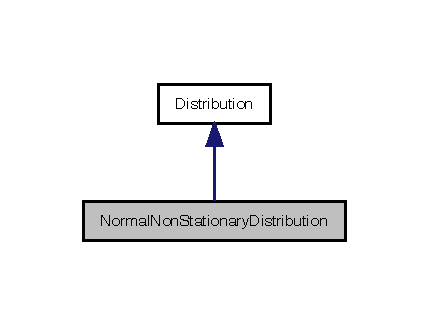
\includegraphics[width=206pt]{class_normal_non_stationary_distribution__inherit__graph}
\end{center}
\end{figure}


Collaboration diagram for Normal\+Non\+Stationary\+Distribution\+:
\nopagebreak
\begin{figure}[H]
\begin{center}
\leavevmode
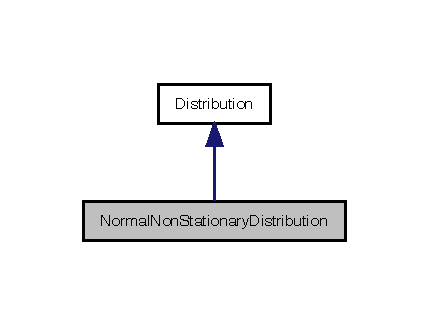
\includegraphics[width=206pt]{class_normal_non_stationary_distribution__coll__graph}
\end{center}
\end{figure}
\subsection*{Public Member Functions}
\begin{DoxyCompactItemize}
\item 
\mbox{\hyperlink{class_normal_non_stationary_distribution_af5868a94c11a8e13d78684160feac9d3}{Normal\+Non\+Stationary\+Distribution}} (string \mbox{\hyperlink{class_distribution_ab3b7be02f0401cb76beb2e744b6161f9}{name}}, vector$<$ double $>$ \&means, vector$<$ double $>$ \&stddevs, vector$<$ int $>$ \&ends, boost\+::mt19937 \&\mbox{\hyperlink{class_distribution_ac8915a45ce85ab6b7506fa42bb850a89}{rng}})
\item 
double \mbox{\hyperlink{class_normal_non_stationary_distribution_a0bd7d418784487c822c330f2b51a6112}{draw}} (int timestep) override
\item 
string \mbox{\hyperlink{class_normal_non_stationary_distribution_a4f2f7cdfacf8b54a0cb2b5237213a693}{to\+File}} () override
\begin{DoxyCompactList}\small\item\em build a representation of this \mbox{\hyperlink{class_distribution}{Distribution}} so that it can be printed to a file and be later analysed by another script \end{DoxyCompactList}\item 
double \mbox{\hyperlink{class_normal_non_stationary_distribution_ae3d2f4fb0e5c9b706c84d05ac14de2aa}{get\+\_\+mean}} (int timestep) override
\end{DoxyCompactItemize}
\subsection*{Additional Inherited Members}


\subsection{Detailed Description}
\mbox{\hyperlink{class_distribution}{Distribution}} of a non-\/stationary normal distribution. 


\begin{DoxyParams}{Parameters}
{\em name} & string, id of the distribution \\
\hline
{\em means} & vector$<$double$>$\&, the means of the normal distributions in the time slots \\
\hline
{\em stddevs} & vector$<$double$>$\&, the stddevs of the normal distributions in the time slots \\
\hline
{\em ends} & vector$<$double$>$\&, the last timestep of each time slot \\
\hline
{\em rng} & boost\+::mt19937\&, rng used to generate data \\
\hline
\end{DoxyParams}


\subsection{Constructor \& Destructor Documentation}
\mbox{\Hypertarget{class_normal_non_stationary_distribution_af5868a94c11a8e13d78684160feac9d3}\label{class_normal_non_stationary_distribution_af5868a94c11a8e13d78684160feac9d3}} 
\index{Normal\+Non\+Stationary\+Distribution@{Normal\+Non\+Stationary\+Distribution}!Normal\+Non\+Stationary\+Distribution@{Normal\+Non\+Stationary\+Distribution}}
\index{Normal\+Non\+Stationary\+Distribution@{Normal\+Non\+Stationary\+Distribution}!Normal\+Non\+Stationary\+Distribution@{Normal\+Non\+Stationary\+Distribution}}
\subsubsection{\texorpdfstring{Normal\+Non\+Stationary\+Distribution()}{NormalNonStationaryDistribution()}}
{\footnotesize\ttfamily Normal\+Non\+Stationary\+Distribution\+::\+Normal\+Non\+Stationary\+Distribution (\begin{DoxyParamCaption}\item[{string}]{name,  }\item[{vector$<$ double $>$ \&}]{means,  }\item[{vector$<$ double $>$ \&}]{stddevs,  }\item[{vector$<$ int $>$ \&}]{ends,  }\item[{boost\+::mt19937 \&}]{rng }\end{DoxyParamCaption})}


\begin{DoxyParams}{Parameters}
{\em name} & string, id of the distribution \\
\hline
{\em means} & vector$<$double$>$\&, the means of the normal distributions in the time slots \\
\hline
{\em stddevs} & vector$<$double$>$\&, the stddevs of the normal distributions in the time slots \\
\hline
{\em ends} & vector$<$double$>$\&, the last timestep of each time slot \\
\hline
{\em rng} & boost\+::mt19937\&, rng used to generate data \\
\hline
\end{DoxyParams}


\subsection{Member Function Documentation}
\mbox{\Hypertarget{class_normal_non_stationary_distribution_a0bd7d418784487c822c330f2b51a6112}\label{class_normal_non_stationary_distribution_a0bd7d418784487c822c330f2b51a6112}} 
\index{Normal\+Non\+Stationary\+Distribution@{Normal\+Non\+Stationary\+Distribution}!draw@{draw}}
\index{draw@{draw}!Normal\+Non\+Stationary\+Distribution@{Normal\+Non\+Stationary\+Distribution}}
\subsubsection{\texorpdfstring{draw()}{draw()}}
{\footnotesize\ttfamily double Normal\+Non\+Stationary\+Distribution\+::draw (\begin{DoxyParamCaption}\item[{int}]{timestep }\end{DoxyParamCaption})\hspace{0.3cm}{\ttfamily [override]}, {\ttfamily [virtual]}}


\begin{DoxyParams}{Parameters}
{\em timestep} & int, timestep at which the reward is drawn \\
\hline
\end{DoxyParams}
\begin{DoxyReturn}{Returns}
a double which is the drawn reward 
\end{DoxyReturn}


Implements \mbox{\hyperlink{class_distribution_a742b398af4a461243028cce3c47d8080}{Distribution}}.

\mbox{\Hypertarget{class_normal_non_stationary_distribution_ae3d2f4fb0e5c9b706c84d05ac14de2aa}\label{class_normal_non_stationary_distribution_ae3d2f4fb0e5c9b706c84d05ac14de2aa}} 
\index{Normal\+Non\+Stationary\+Distribution@{Normal\+Non\+Stationary\+Distribution}!get\+\_\+mean@{get\+\_\+mean}}
\index{get\+\_\+mean@{get\+\_\+mean}!Normal\+Non\+Stationary\+Distribution@{Normal\+Non\+Stationary\+Distribution}}
\subsubsection{\texorpdfstring{get\+\_\+mean()}{get\_mean()}}
{\footnotesize\ttfamily double Normal\+Non\+Stationary\+Distribution\+::get\+\_\+mean (\begin{DoxyParamCaption}\item[{int}]{timestep }\end{DoxyParamCaption})\hspace{0.3cm}{\ttfamily [override]}, {\ttfamily [virtual]}}


\begin{DoxyParams}{Parameters}
{\em timestep} & integer, the timestep at which the mean is asked \\
\hline
\end{DoxyParams}
\begin{DoxyReturn}{Returns}
the mean (double) at the specified timestep 
\end{DoxyReturn}


Implements \mbox{\hyperlink{class_distribution_ac9c74d18549f532caa09ae86d8b25b55}{Distribution}}.

\mbox{\Hypertarget{class_normal_non_stationary_distribution_a4f2f7cdfacf8b54a0cb2b5237213a693}\label{class_normal_non_stationary_distribution_a4f2f7cdfacf8b54a0cb2b5237213a693}} 
\index{Normal\+Non\+Stationary\+Distribution@{Normal\+Non\+Stationary\+Distribution}!to\+File@{to\+File}}
\index{to\+File@{to\+File}!Normal\+Non\+Stationary\+Distribution@{Normal\+Non\+Stationary\+Distribution}}
\subsubsection{\texorpdfstring{to\+File()}{toFile()}}
{\footnotesize\ttfamily string Normal\+Non\+Stationary\+Distribution\+::to\+File (\begin{DoxyParamCaption}{ }\end{DoxyParamCaption})\hspace{0.3cm}{\ttfamily [override]}, {\ttfamily [virtual]}}



build a representation of this \mbox{\hyperlink{class_distribution}{Distribution}} so that it can be printed to a file and be later analysed by another script 

\begin{DoxyReturn}{Returns}
a string that represents this \mbox{\hyperlink{class_distribution}{Distribution}} 
\end{DoxyReturn}


Implements \mbox{\hyperlink{class_distribution_ac41d57a4d7f82041810f886590a236a5}{Distribution}}.



The documentation for this class was generated from the following files\+:\begin{DoxyCompactItemize}
\item 
src/\mbox{\hyperlink{distribution_8h}{distribution.\+h}}\item 
src/\mbox{\hyperlink{distribution_8cpp}{distribution.\+cpp}}\end{DoxyCompactItemize}

\hypertarget{class_per_arm_c_t_s}{}\section{Per\+Arm\+C\+TS Class Reference}
\label{class_per_arm_c_t_s}\index{Per\+Arm\+C\+TS@{Per\+Arm\+C\+TS}}


Thompson Sampling with prior on runlength distribution. \mbox{\hyperlink{class_distribution}{Distribution}} changes are assumed to happen locally (all arms are not assumed to change at the same timestep)  




{\ttfamily \#include $<$thompsonsampling.\+h$>$}



Inheritance diagram for Per\+Arm\+C\+TS\+:
\nopagebreak
\begin{figure}[H]
\begin{center}
\leavevmode
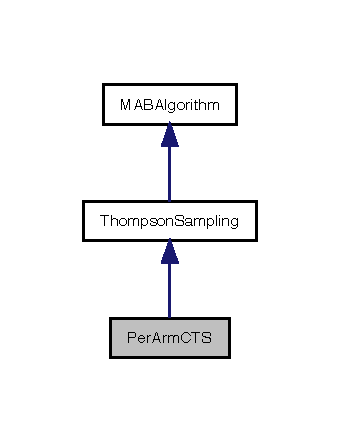
\includegraphics[width=163pt]{class_per_arm_c_t_s__inherit__graph}
\end{center}
\end{figure}


Collaboration diagram for Per\+Arm\+C\+TS\+:
\nopagebreak
\begin{figure}[H]
\begin{center}
\leavevmode
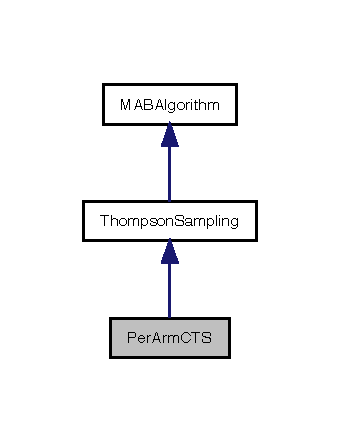
\includegraphics[width=163pt]{class_per_arm_c_t_s__coll__graph}
\end{center}
\end{figure}
\subsection*{Public Member Functions}
\begin{DoxyCompactItemize}
\item 
\mbox{\hyperlink{class_per_arm_c_t_s_a87170c6aefd052d6ea8bb20866f6f32e}{Per\+Arm\+C\+TS}} (string \mbox{\hyperlink{class_m_a_b_algorithm_a77b10ecc4b49d519c557f65358167b82}{name}}, int \mbox{\hyperlink{class_m_a_b_algorithm_a340fa9e83e85b092f2c6125fc4e8549b}{num\+\_\+of\+\_\+arms}}, boost\+::mt19937 \&\mbox{\hyperlink{class_thompson_sampling_a1b66efa9bb0912df92975147f8923216}{rng}}, double gamma)
\item 
int \mbox{\hyperlink{class_per_arm_c_t_s_ab8904bef227b13aed75aade589421c5a}{choose\+\_\+action}} () override
\item 
void \mbox{\hyperlink{class_per_arm_c_t_s_af9ac7b45d329223ce506e977b96a32ee}{receive\+\_\+reward}} (double reward, int pulled\+\_\+arm) override
\begin{DoxyCompactList}\small\item\em Update the internal variables of the algorithm according to the new received reward. \end{DoxyCompactList}\item 
void \mbox{\hyperlink{class_per_arm_c_t_s_ae5f8998bfb68b4a9cbdea7bca34f5cbe}{reset}} (int action=-\/1) override
\begin{DoxyCompactList}\small\item\em resets the internal variables of the algorithm \end{DoxyCompactList}\end{DoxyCompactItemize}
\subsection*{Additional Inherited Members}


\subsection{Detailed Description}
Thompson Sampling with prior on runlength distribution. \mbox{\hyperlink{class_distribution}{Distribution}} changes are assumed to happen locally (all arms are not assumed to change at the same timestep) 

\subsection{Constructor \& Destructor Documentation}
\mbox{\Hypertarget{class_per_arm_c_t_s_a87170c6aefd052d6ea8bb20866f6f32e}\label{class_per_arm_c_t_s_a87170c6aefd052d6ea8bb20866f6f32e}} 
\index{Per\+Arm\+C\+TS@{Per\+Arm\+C\+TS}!Per\+Arm\+C\+TS@{Per\+Arm\+C\+TS}}
\index{Per\+Arm\+C\+TS@{Per\+Arm\+C\+TS}!Per\+Arm\+C\+TS@{Per\+Arm\+C\+TS}}
\subsubsection{\texorpdfstring{Per\+Arm\+C\+T\+S()}{PerArmCTS()}}
{\footnotesize\ttfamily Per\+Arm\+C\+T\+S\+::\+Per\+Arm\+C\+TS (\begin{DoxyParamCaption}\item[{string}]{name,  }\item[{int}]{num\+\_\+of\+\_\+arms,  }\item[{boost\+::mt19937 \&}]{rng,  }\item[{double}]{gamma }\end{DoxyParamCaption})}


\begin{DoxyParams}{Parameters}
{\em name} & string, id of the algorithm \\
\hline
{\em num\+\_\+of\+\_\+arms} & integer, number of arms the algorithm will work on \\
\hline
{\em rng} & boost\+::mt19937\&, random number generator \\
\hline
{\em gamma} & double, parameter of the prior of the geometric runlength distribution \\
\hline
\end{DoxyParams}


\subsection{Member Function Documentation}
\mbox{\Hypertarget{class_per_arm_c_t_s_ab8904bef227b13aed75aade589421c5a}\label{class_per_arm_c_t_s_ab8904bef227b13aed75aade589421c5a}} 
\index{Per\+Arm\+C\+TS@{Per\+Arm\+C\+TS}!choose\+\_\+action@{choose\+\_\+action}}
\index{choose\+\_\+action@{choose\+\_\+action}!Per\+Arm\+C\+TS@{Per\+Arm\+C\+TS}}
\subsubsection{\texorpdfstring{choose\+\_\+action()}{choose\_action()}}
{\footnotesize\ttfamily int Per\+Arm\+C\+T\+S\+::choose\+\_\+action (\begin{DoxyParamCaption}{ }\end{DoxyParamCaption})\hspace{0.3cm}{\ttfamily [override]}, {\ttfamily [virtual]}}

\begin{DoxyReturn}{Returns}
an integer representing the chosen arm 
\end{DoxyReturn}


Implements \mbox{\hyperlink{class_m_a_b_algorithm_afb48f01df0e1860d19759f6e20335007}{M\+A\+B\+Algorithm}}.

\mbox{\Hypertarget{class_per_arm_c_t_s_af9ac7b45d329223ce506e977b96a32ee}\label{class_per_arm_c_t_s_af9ac7b45d329223ce506e977b96a32ee}} 
\index{Per\+Arm\+C\+TS@{Per\+Arm\+C\+TS}!receive\+\_\+reward@{receive\+\_\+reward}}
\index{receive\+\_\+reward@{receive\+\_\+reward}!Per\+Arm\+C\+TS@{Per\+Arm\+C\+TS}}
\subsubsection{\texorpdfstring{receive\+\_\+reward()}{receive\_reward()}}
{\footnotesize\ttfamily void Per\+Arm\+C\+T\+S\+::receive\+\_\+reward (\begin{DoxyParamCaption}\item[{double}]{reward,  }\item[{int}]{pulled\+\_\+arm }\end{DoxyParamCaption})\hspace{0.3cm}{\ttfamily [override]}, {\ttfamily [virtual]}}



Update the internal variables of the algorithm according to the new received reward. 


\begin{DoxyParams}{Parameters}
{\em reward} & double, new received reward \\
\hline
{\em pulled\+\_\+arm} & integer, represents the pulled arm \\
\hline
\end{DoxyParams}


Reimplemented from \mbox{\hyperlink{class_m_a_b_algorithm_aa584b3d6b86fa050e3389be9781b5782}{M\+A\+B\+Algorithm}}.

\mbox{\Hypertarget{class_per_arm_c_t_s_ae5f8998bfb68b4a9cbdea7bca34f5cbe}\label{class_per_arm_c_t_s_ae5f8998bfb68b4a9cbdea7bca34f5cbe}} 
\index{Per\+Arm\+C\+TS@{Per\+Arm\+C\+TS}!reset@{reset}}
\index{reset@{reset}!Per\+Arm\+C\+TS@{Per\+Arm\+C\+TS}}
\subsubsection{\texorpdfstring{reset()}{reset()}}
{\footnotesize\ttfamily void Per\+Arm\+C\+T\+S\+::reset (\begin{DoxyParamCaption}\item[{int}]{action = {\ttfamily -\/1} }\end{DoxyParamCaption})\hspace{0.3cm}{\ttfamily [override]}, {\ttfamily [virtual]}}



resets the internal variables of the algorithm 


\begin{DoxyParams}{Parameters}
{\em action} & integer, specifies which variables to reset. If in (0, num\+\_\+of\+\_\+arms -\/ 1), then it resets only the info related to such arm. If == -\/1, resets all the arms. \\
\hline
\end{DoxyParams}


Reimplemented from \mbox{\hyperlink{class_m_a_b_algorithm_ad5761cee0b0e3421d1f043dbcc0b5f85}{M\+A\+B\+Algorithm}}.



The documentation for this class was generated from the following files\+:\begin{DoxyCompactItemize}
\item 
src/\mbox{\hyperlink{thompsonsampling_8h}{thompsonsampling.\+h}}\item 
src/\mbox{\hyperlink{thompsonsampling_8cpp}{thompsonsampling.\+cpp}}\end{DoxyCompactItemize}

\hypertarget{class_plotter}{}\section{Plotter Class Reference}
\label{class_plotter}\index{Plotter@{Plotter}}


Class adept at plotting the results of the experiments.  




{\ttfamily \#include $<$plotter.\+h$>$}

\subsection*{Static Public Member Functions}
\begin{DoxyCompactItemize}
\item 
static void \mbox{\hyperlink{class_plotter_af025f4f67616c710d73498541cc1c08c}{plot\+\_\+experiments}} ()
\begin{DoxyCompactList}\small\item\em plots the results of the experiments inside iìthe images folder \end{DoxyCompactList}\end{DoxyCompactItemize}


\subsection{Detailed Description}
Class adept at plotting the results of the experiments. 

\subsection{Member Function Documentation}
\mbox{\Hypertarget{class_plotter_af025f4f67616c710d73498541cc1c08c}\label{class_plotter_af025f4f67616c710d73498541cc1c08c}} 
\index{Plotter@{Plotter}!plot\+\_\+experiments@{plot\+\_\+experiments}}
\index{plot\+\_\+experiments@{plot\+\_\+experiments}!Plotter@{Plotter}}
\subsubsection{\texorpdfstring{plot\+\_\+experiments()}{plot\_experiments()}}
{\footnotesize\ttfamily void Plotter\+::plot\+\_\+experiments (\begin{DoxyParamCaption}{ }\end{DoxyParamCaption})\hspace{0.3cm}{\ttfamily [static]}}



plots the results of the experiments inside iìthe images folder 



The documentation for this class was generated from the following files\+:\begin{DoxyCompactItemize}
\item 
src/\mbox{\hyperlink{plotter_8h}{plotter.\+h}}\item 
src/\mbox{\hyperlink{plotter_8cpp}{plotter.\+cpp}}\end{DoxyCompactItemize}

\hypertarget{class_r_e_x_p3}{}\section{R\+E\+X\+P3 Class Reference}
\label{class_r_e_x_p3}\index{R\+E\+X\+P3@{R\+E\+X\+P3}}


\mbox{\hyperlink{class_r_e_x_p3}{R\+E\+X\+P3}} algorithm.  




{\ttfamily \#include $<$exp.\+h$>$}



Inheritance diagram for R\+E\+X\+P3\+:
\nopagebreak
\begin{figure}[H]
\begin{center}
\leavevmode
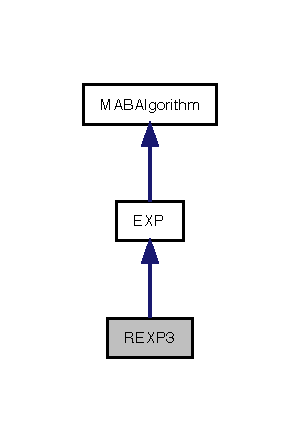
\includegraphics[width=144pt]{class_r_e_x_p3__inherit__graph}
\end{center}
\end{figure}


Collaboration diagram for R\+E\+X\+P3\+:
\nopagebreak
\begin{figure}[H]
\begin{center}
\leavevmode
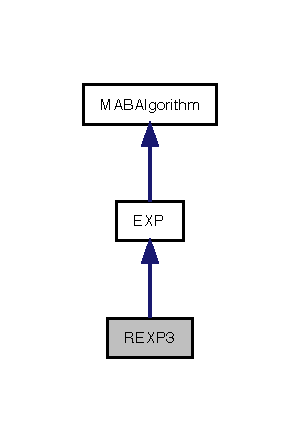
\includegraphics[width=144pt]{class_r_e_x_p3__coll__graph}
\end{center}
\end{figure}
\subsection*{Public Member Functions}
\begin{DoxyCompactItemize}
\item 
\mbox{\hyperlink{class_r_e_x_p3_a6b676721455094e28bea43920fa024e4}{R\+E\+X\+P3}} (string \mbox{\hyperlink{class_m_a_b_algorithm_a77b10ecc4b49d519c557f65358167b82}{name}}, int \mbox{\hyperlink{class_m_a_b_algorithm_a340fa9e83e85b092f2c6125fc4e8549b}{num\+\_\+of\+\_\+arms}}, double beta, int window\+\_\+size)
\begin{DoxyCompactList}\small\item\em constructor of \mbox{\hyperlink{class_r_e_x_p3}{R\+E\+X\+P3}} \end{DoxyCompactList}\item 
int \mbox{\hyperlink{class_r_e_x_p3_aba9cbcdc74602157701b022a7758d584}{choose\+\_\+action}} () override
\item 
void \mbox{\hyperlink{class_r_e_x_p3_a535d6667ecfa71568a68a5a09c44d4bf}{receive\+\_\+reward}} (double reward, int pulled\+\_\+arm) override
\begin{DoxyCompactList}\small\item\em Update the internal variables of the algorithm according to the new received reward. \end{DoxyCompactList}\item 
void \mbox{\hyperlink{class_r_e_x_p3_ad99a97c07f75addc64e612774de81307}{reset}} (int action=-\/1) override
\begin{DoxyCompactList}\small\item\em resets the internal variables of the algorithm \end{DoxyCompactList}\end{DoxyCompactItemize}
\subsection*{Additional Inherited Members}


\subsection{Detailed Description}
\mbox{\hyperlink{class_r_e_x_p3}{R\+E\+X\+P3}} algorithm. 

\subsection{Constructor \& Destructor Documentation}
\mbox{\Hypertarget{class_r_e_x_p3_a6b676721455094e28bea43920fa024e4}\label{class_r_e_x_p3_a6b676721455094e28bea43920fa024e4}} 
\index{R\+E\+X\+P3@{R\+E\+X\+P3}!R\+E\+X\+P3@{R\+E\+X\+P3}}
\index{R\+E\+X\+P3@{R\+E\+X\+P3}!R\+E\+X\+P3@{R\+E\+X\+P3}}
\subsubsection{\texorpdfstring{R\+E\+X\+P3()}{REXP3()}}
{\footnotesize\ttfamily R\+E\+X\+P3\+::\+R\+E\+X\+P3 (\begin{DoxyParamCaption}\item[{string}]{name,  }\item[{int}]{num\+\_\+of\+\_\+arms,  }\item[{double}]{beta,  }\item[{int}]{window\+\_\+size }\end{DoxyParamCaption})}



constructor of \mbox{\hyperlink{class_r_e_x_p3}{R\+E\+X\+P3}} 


\begin{DoxyParams}{Parameters}
{\em name} & string, id of the algorithm \\
\hline
{\em num\+\_\+of\+\_\+arms} & integer, number of arms the algorithm will work on \\
\hline
{\em beta} & double, exploration parameter (between 0 and 1) and also exponential update parameter \\
\hline
{\em window\+\_\+size} & integer, window size \\
\hline
\end{DoxyParams}


\subsection{Member Function Documentation}
\mbox{\Hypertarget{class_r_e_x_p3_aba9cbcdc74602157701b022a7758d584}\label{class_r_e_x_p3_aba9cbcdc74602157701b022a7758d584}} 
\index{R\+E\+X\+P3@{R\+E\+X\+P3}!choose\+\_\+action@{choose\+\_\+action}}
\index{choose\+\_\+action@{choose\+\_\+action}!R\+E\+X\+P3@{R\+E\+X\+P3}}
\subsubsection{\texorpdfstring{choose\+\_\+action()}{choose\_action()}}
{\footnotesize\ttfamily int R\+E\+X\+P3\+::choose\+\_\+action (\begin{DoxyParamCaption}{ }\end{DoxyParamCaption})\hspace{0.3cm}{\ttfamily [override]}, {\ttfamily [virtual]}}

\begin{DoxyReturn}{Returns}
an integer representing the chosen arm 
\end{DoxyReturn}


Implements \mbox{\hyperlink{class_m_a_b_algorithm_afb48f01df0e1860d19759f6e20335007}{M\+A\+B\+Algorithm}}.

\mbox{\Hypertarget{class_r_e_x_p3_a535d6667ecfa71568a68a5a09c44d4bf}\label{class_r_e_x_p3_a535d6667ecfa71568a68a5a09c44d4bf}} 
\index{R\+E\+X\+P3@{R\+E\+X\+P3}!receive\+\_\+reward@{receive\+\_\+reward}}
\index{receive\+\_\+reward@{receive\+\_\+reward}!R\+E\+X\+P3@{R\+E\+X\+P3}}
\subsubsection{\texorpdfstring{receive\+\_\+reward()}{receive\_reward()}}
{\footnotesize\ttfamily void R\+E\+X\+P3\+::receive\+\_\+reward (\begin{DoxyParamCaption}\item[{double}]{reward,  }\item[{int}]{pulled\+\_\+arm }\end{DoxyParamCaption})\hspace{0.3cm}{\ttfamily [override]}, {\ttfamily [virtual]}}



Update the internal variables of the algorithm according to the new received reward. 


\begin{DoxyParams}{Parameters}
{\em reward} & double, new received reward \\
\hline
{\em pulled\+\_\+arm} & integer, represents the pulled arm \\
\hline
\end{DoxyParams}


Reimplemented from \mbox{\hyperlink{class_m_a_b_algorithm_aa584b3d6b86fa050e3389be9781b5782}{M\+A\+B\+Algorithm}}.

\mbox{\Hypertarget{class_r_e_x_p3_ad99a97c07f75addc64e612774de81307}\label{class_r_e_x_p3_ad99a97c07f75addc64e612774de81307}} 
\index{R\+E\+X\+P3@{R\+E\+X\+P3}!reset@{reset}}
\index{reset@{reset}!R\+E\+X\+P3@{R\+E\+X\+P3}}
\subsubsection{\texorpdfstring{reset()}{reset()}}
{\footnotesize\ttfamily void R\+E\+X\+P3\+::reset (\begin{DoxyParamCaption}\item[{int}]{action = {\ttfamily -\/1} }\end{DoxyParamCaption})\hspace{0.3cm}{\ttfamily [override]}, {\ttfamily [virtual]}}



resets the internal variables of the algorithm 


\begin{DoxyParams}{Parameters}
{\em action} & integer, specifies which variables to reset. If in (0, num\+\_\+of\+\_\+arms -\/ 1), then it resets only the info related to such arm. If == -\/1, resets all the arms. \\
\hline
\end{DoxyParams}


Reimplemented from \mbox{\hyperlink{class_m_a_b_algorithm_ad5761cee0b0e3421d1f043dbcc0b5f85}{M\+A\+B\+Algorithm}}.



The documentation for this class was generated from the following files\+:\begin{DoxyCompactItemize}
\item 
src/\mbox{\hyperlink{exp_8h}{exp.\+h}}\item 
src/\mbox{\hyperlink{exp_8cpp}{exp.\+cpp}}\end{DoxyCompactItemize}

\hypertarget{class_round___algorithm}{}\section{Round\+\_\+\+Algorithm Class Reference}
\label{class_round___algorithm}\index{Round\+\_\+\+Algorithm@{Round\+\_\+\+Algorithm}}


Meta-\/algorithm which selects each arm once before making its sub-\/algorithm run.  




{\ttfamily \#include $<$meta\+\_\+algorithms.\+h$>$}



Inheritance diagram for Round\+\_\+\+Algorithm\+:
\nopagebreak
\begin{figure}[H]
\begin{center}
\leavevmode
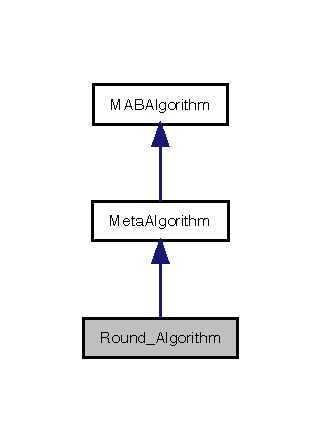
\includegraphics[width=154pt]{class_round___algorithm__inherit__graph}
\end{center}
\end{figure}


Collaboration diagram for Round\+\_\+\+Algorithm\+:
\nopagebreak
\begin{figure}[H]
\begin{center}
\leavevmode
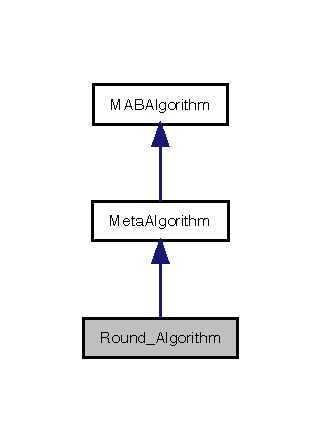
\includegraphics[width=154pt]{class_round___algorithm__coll__graph}
\end{center}
\end{figure}
\subsection*{Public Member Functions}
\begin{DoxyCompactItemize}
\item 
\mbox{\hyperlink{class_round___algorithm_abf6d3592abbbc873a002238be60399e6}{Round\+\_\+\+Algorithm}} (string \mbox{\hyperlink{class_m_a_b_algorithm_a77b10ecc4b49d519c557f65358167b82}{name}}, int \mbox{\hyperlink{class_m_a_b_algorithm_a340fa9e83e85b092f2c6125fc4e8549b}{num\+\_\+of\+\_\+arms}}, string sub\+\_\+alg\+\_\+line, boost\+::mt19937 \&rng)
\item 
virtual int \mbox{\hyperlink{class_round___algorithm_a019a9a7a564a49512f5089c3829e6f4e}{choose\+\_\+action}} () override
\item 
virtual void \mbox{\hyperlink{class_round___algorithm_a945da188a51c00d1923f4eb8434042eb}{receive\+\_\+reward}} (double reward, int pulled\+\_\+arm) override
\begin{DoxyCompactList}\small\item\em Update the internal variables of the algorithm according to the new received reward. \end{DoxyCompactList}\item 
virtual void \mbox{\hyperlink{class_round___algorithm_ae2c21984dbd89f5ba1a4f530472cf7f7}{reset}} (int action=-\/1) override
\begin{DoxyCompactList}\small\item\em resets the internal variables of the algorithm \end{DoxyCompactList}\end{DoxyCompactItemize}
\subsection*{Additional Inherited Members}


\subsection{Detailed Description}
Meta-\/algorithm which selects each arm once before making its sub-\/algorithm run. 

\subsection{Constructor \& Destructor Documentation}
\mbox{\Hypertarget{class_round___algorithm_abf6d3592abbbc873a002238be60399e6}\label{class_round___algorithm_abf6d3592abbbc873a002238be60399e6}} 
\index{Round\+\_\+\+Algorithm@{Round\+\_\+\+Algorithm}!Round\+\_\+\+Algorithm@{Round\+\_\+\+Algorithm}}
\index{Round\+\_\+\+Algorithm@{Round\+\_\+\+Algorithm}!Round\+\_\+\+Algorithm@{Round\+\_\+\+Algorithm}}
\subsubsection{\texorpdfstring{Round\+\_\+\+Algorithm()}{Round\_Algorithm()}}
{\footnotesize\ttfamily Round\+\_\+\+Algorithm\+::\+Round\+\_\+\+Algorithm (\begin{DoxyParamCaption}\item[{string}]{name,  }\item[{int}]{num\+\_\+of\+\_\+arms,  }\item[{string}]{sub\+\_\+alg\+\_\+line,  }\item[{boost\+::mt19937 \&}]{rng }\end{DoxyParamCaption})}


\begin{DoxyParams}{Parameters}
{\em name} & string, id of the algorithm \\
\hline
{\em num\+\_\+of\+\_\+arms} & integer, number of arms the algorithm will work with \\
\hline
{\em sub\+\_\+alg\+\_\+line} & string, specification of the sub-\/algorithm \\
\hline
{\em rng} & boost\+::mt19937\&, random number generator \\
\hline
\end{DoxyParams}


\subsection{Member Function Documentation}
\mbox{\Hypertarget{class_round___algorithm_a019a9a7a564a49512f5089c3829e6f4e}\label{class_round___algorithm_a019a9a7a564a49512f5089c3829e6f4e}} 
\index{Round\+\_\+\+Algorithm@{Round\+\_\+\+Algorithm}!choose\+\_\+action@{choose\+\_\+action}}
\index{choose\+\_\+action@{choose\+\_\+action}!Round\+\_\+\+Algorithm@{Round\+\_\+\+Algorithm}}
\subsubsection{\texorpdfstring{choose\+\_\+action()}{choose\_action()}}
{\footnotesize\ttfamily int Round\+\_\+\+Algorithm\+::choose\+\_\+action (\begin{DoxyParamCaption}{ }\end{DoxyParamCaption})\hspace{0.3cm}{\ttfamily [override]}, {\ttfamily [virtual]}}

\begin{DoxyReturn}{Returns}
an integer representing the chosen arm 
\end{DoxyReturn}


Implements \mbox{\hyperlink{class_m_a_b_algorithm_afb48f01df0e1860d19759f6e20335007}{M\+A\+B\+Algorithm}}.

\mbox{\Hypertarget{class_round___algorithm_a945da188a51c00d1923f4eb8434042eb}\label{class_round___algorithm_a945da188a51c00d1923f4eb8434042eb}} 
\index{Round\+\_\+\+Algorithm@{Round\+\_\+\+Algorithm}!receive\+\_\+reward@{receive\+\_\+reward}}
\index{receive\+\_\+reward@{receive\+\_\+reward}!Round\+\_\+\+Algorithm@{Round\+\_\+\+Algorithm}}
\subsubsection{\texorpdfstring{receive\+\_\+reward()}{receive\_reward()}}
{\footnotesize\ttfamily void Round\+\_\+\+Algorithm\+::receive\+\_\+reward (\begin{DoxyParamCaption}\item[{double}]{reward,  }\item[{int}]{pulled\+\_\+arm }\end{DoxyParamCaption})\hspace{0.3cm}{\ttfamily [override]}, {\ttfamily [virtual]}}



Update the internal variables of the algorithm according to the new received reward. 


\begin{DoxyParams}{Parameters}
{\em reward} & double, new received reward \\
\hline
{\em pulled\+\_\+arm} & integer, represents the pulled arm \\
\hline
\end{DoxyParams}


Reimplemented from \mbox{\hyperlink{class_m_a_b_algorithm_aa584b3d6b86fa050e3389be9781b5782}{M\+A\+B\+Algorithm}}.

\mbox{\Hypertarget{class_round___algorithm_ae2c21984dbd89f5ba1a4f530472cf7f7}\label{class_round___algorithm_ae2c21984dbd89f5ba1a4f530472cf7f7}} 
\index{Round\+\_\+\+Algorithm@{Round\+\_\+\+Algorithm}!reset@{reset}}
\index{reset@{reset}!Round\+\_\+\+Algorithm@{Round\+\_\+\+Algorithm}}
\subsubsection{\texorpdfstring{reset()}{reset()}}
{\footnotesize\ttfamily void Round\+\_\+\+Algorithm\+::reset (\begin{DoxyParamCaption}\item[{int}]{action = {\ttfamily -\/1} }\end{DoxyParamCaption})\hspace{0.3cm}{\ttfamily [override]}, {\ttfamily [virtual]}}



resets the internal variables of the algorithm 


\begin{DoxyParams}{Parameters}
{\em action} & integer, specifies which variables to reset. If in (0, num\+\_\+of\+\_\+arms -\/ 1), then it resets only the info related to such arm. If == -\/1, resets all the arms. \\
\hline
\end{DoxyParams}


Reimplemented from \mbox{\hyperlink{class_m_a_b_algorithm_ad5761cee0b0e3421d1f043dbcc0b5f85}{M\+A\+B\+Algorithm}}.



The documentation for this class was generated from the following files\+:\begin{DoxyCompactItemize}
\item 
src/\mbox{\hyperlink{meta__algorithms_8h}{meta\+\_\+algorithms.\+h}}\item 
src/\mbox{\hyperlink{meta__algorithms_8cpp}{meta\+\_\+algorithms.\+cpp}}\end{DoxyCompactItemize}

\hypertarget{class_square_wave_distribution}{}\section{Square\+Wave\+Distribution Class Reference}
\label{class_square_wave_distribution}\index{Square\+Wave\+Distribution@{Square\+Wave\+Distribution}}


\mbox{\hyperlink{class_distribution}{Distribution}} equivalent to a \mbox{\hyperlink{class_fixed_non_stationary_distribution}{Fixed\+Non\+Stationary\+Distribution}} where the mean flips between 0 and v at each timestep.  




{\ttfamily \#include $<$distribution.\+h$>$}



Inheritance diagram for Square\+Wave\+Distribution\+:
\nopagebreak
\begin{figure}[H]
\begin{center}
\leavevmode
\includegraphics[width=177pt]{class_square_wave_distribution__inherit__graph}
\end{center}
\end{figure}


Collaboration diagram for Square\+Wave\+Distribution\+:
\nopagebreak
\begin{figure}[H]
\begin{center}
\leavevmode
\includegraphics[width=177pt]{class_square_wave_distribution__coll__graph}
\end{center}
\end{figure}
\subsection*{Public Member Functions}
\begin{DoxyCompactItemize}
\item 
\mbox{\hyperlink{class_square_wave_distribution_acb93b13cc90da11d5297ce577c24aed7}{Square\+Wave\+Distribution}} (string \mbox{\hyperlink{class_distribution_ab3b7be02f0401cb76beb2e744b6161f9}{name}}, double v, double cur\+\_\+v, boost\+::mt19937 \&\mbox{\hyperlink{class_distribution_ac8915a45ce85ab6b7506fa42bb850a89}{rng}})
\item 
double \mbox{\hyperlink{class_square_wave_distribution_a7994182585346203ec158272cc39b17e}{draw}} (int timestep) override
\item 
string \mbox{\hyperlink{class_square_wave_distribution_a8ba3fbbf02f23f02697f34f841e9a870}{to\+File}} () override
\begin{DoxyCompactList}\small\item\em build a representation of this \mbox{\hyperlink{class_distribution}{Distribution}} so that it can be printed to a file and be later analysed by another script \end{DoxyCompactList}\item 
double \mbox{\hyperlink{class_square_wave_distribution_ac2e790a852c02473e70e4ff5090cfc51}{get\+\_\+mean}} (int timestep) override
\end{DoxyCompactItemize}
\subsection*{Additional Inherited Members}


\subsection{Detailed Description}
\mbox{\hyperlink{class_distribution}{Distribution}} equivalent to a \mbox{\hyperlink{class_fixed_non_stationary_distribution}{Fixed\+Non\+Stationary\+Distribution}} where the mean flips between 0 and v at each timestep. 


\begin{DoxyParams}{Parameters}
{\em name} & string, id of the distribution \\
\hline
{\em v} & double, value of the distribution other than zero \\
\hline
{\em cur\+\_\+v} & double, first value that the distribution will returns \\
\hline
{\em rng} & boost\+::mt19937\&, rng used to generate data \\
\hline
\end{DoxyParams}


\subsection{Constructor \& Destructor Documentation}
\mbox{\Hypertarget{class_square_wave_distribution_acb93b13cc90da11d5297ce577c24aed7}\label{class_square_wave_distribution_acb93b13cc90da11d5297ce577c24aed7}} 
\index{Square\+Wave\+Distribution@{Square\+Wave\+Distribution}!Square\+Wave\+Distribution@{Square\+Wave\+Distribution}}
\index{Square\+Wave\+Distribution@{Square\+Wave\+Distribution}!Square\+Wave\+Distribution@{Square\+Wave\+Distribution}}
\subsubsection{\texorpdfstring{Square\+Wave\+Distribution()}{SquareWaveDistribution()}}
{\footnotesize\ttfamily Square\+Wave\+Distribution\+::\+Square\+Wave\+Distribution (\begin{DoxyParamCaption}\item[{string}]{name,  }\item[{double}]{v,  }\item[{double}]{cur\+\_\+v,  }\item[{boost\+::mt19937 \&}]{rng }\end{DoxyParamCaption})}


\begin{DoxyParams}{Parameters}
{\em name} & string, id of the distribution \\
\hline
{\em v} & double, value of the distribution other than zero \\
\hline
{\em cur\+\_\+v} & double, first value that the distribution will returns \\
\hline
{\em rng} & boost\+::mt19937\&, rng used to generate data \\
\hline
\end{DoxyParams}


\subsection{Member Function Documentation}
\mbox{\Hypertarget{class_square_wave_distribution_a7994182585346203ec158272cc39b17e}\label{class_square_wave_distribution_a7994182585346203ec158272cc39b17e}} 
\index{Square\+Wave\+Distribution@{Square\+Wave\+Distribution}!draw@{draw}}
\index{draw@{draw}!Square\+Wave\+Distribution@{Square\+Wave\+Distribution}}
\subsubsection{\texorpdfstring{draw()}{draw()}}
{\footnotesize\ttfamily double Square\+Wave\+Distribution\+::draw (\begin{DoxyParamCaption}\item[{int}]{timestep }\end{DoxyParamCaption})\hspace{0.3cm}{\ttfamily [override]}, {\ttfamily [virtual]}}


\begin{DoxyParams}{Parameters}
{\em timestep} & int, timestep at which the reward is drawn \\
\hline
\end{DoxyParams}
\begin{DoxyReturn}{Returns}
a double which is the drawn reward 
\end{DoxyReturn}


Implements \mbox{\hyperlink{class_distribution_a742b398af4a461243028cce3c47d8080}{Distribution}}.

\mbox{\Hypertarget{class_square_wave_distribution_ac2e790a852c02473e70e4ff5090cfc51}\label{class_square_wave_distribution_ac2e790a852c02473e70e4ff5090cfc51}} 
\index{Square\+Wave\+Distribution@{Square\+Wave\+Distribution}!get\+\_\+mean@{get\+\_\+mean}}
\index{get\+\_\+mean@{get\+\_\+mean}!Square\+Wave\+Distribution@{Square\+Wave\+Distribution}}
\subsubsection{\texorpdfstring{get\+\_\+mean()}{get\_mean()}}
{\footnotesize\ttfamily double Square\+Wave\+Distribution\+::get\+\_\+mean (\begin{DoxyParamCaption}\item[{int}]{timestep }\end{DoxyParamCaption})\hspace{0.3cm}{\ttfamily [override]}, {\ttfamily [virtual]}}


\begin{DoxyParams}{Parameters}
{\em timestep} & integer, the timestep at which the mean is asked \\
\hline
\end{DoxyParams}
\begin{DoxyReturn}{Returns}
the mean (double) at the specified timestep 
\end{DoxyReturn}


Implements \mbox{\hyperlink{class_distribution_ac9c74d18549f532caa09ae86d8b25b55}{Distribution}}.

\mbox{\Hypertarget{class_square_wave_distribution_a8ba3fbbf02f23f02697f34f841e9a870}\label{class_square_wave_distribution_a8ba3fbbf02f23f02697f34f841e9a870}} 
\index{Square\+Wave\+Distribution@{Square\+Wave\+Distribution}!to\+File@{to\+File}}
\index{to\+File@{to\+File}!Square\+Wave\+Distribution@{Square\+Wave\+Distribution}}
\subsubsection{\texorpdfstring{to\+File()}{toFile()}}
{\footnotesize\ttfamily string Square\+Wave\+Distribution\+::to\+File (\begin{DoxyParamCaption}{ }\end{DoxyParamCaption})\hspace{0.3cm}{\ttfamily [override]}, {\ttfamily [virtual]}}



build a representation of this \mbox{\hyperlink{class_distribution}{Distribution}} so that it can be printed to a file and be later analysed by another script 

\begin{DoxyReturn}{Returns}
a string that represents this \mbox{\hyperlink{class_distribution}{Distribution}} 
\end{DoxyReturn}


Implements \mbox{\hyperlink{class_distribution_ac41d57a4d7f82041810f886590a236a5}{Distribution}}.



The documentation for this class was generated from the following files\+:\begin{DoxyCompactItemize}
\item 
src/\mbox{\hyperlink{distribution_8h}{distribution.\+h}}\item 
src/\mbox{\hyperlink{distribution_8cpp}{distribution.\+cpp}}\end{DoxyCompactItemize}

\hypertarget{class_statistic_manager}{}\section{Statistic\+Manager Class Reference}
\label{class_statistic_manager}\index{Statistic\+Manager@{Statistic\+Manager}}


Class that saves all the statistics of an experiment and save them in some files.  




{\ttfamily \#include $<$statistic\+\_\+manager.\+h$>$}

\subsection*{Public Member Functions}
\begin{DoxyCompactItemize}
\item 
\mbox{\hyperlink{class_statistic_manager_a7791d6be8cb2cc1b61f7329e94c541dc}{Statistic\+Manager}} (string name, \mbox{\hyperlink{class_m_a_b}{M\+AB}} $\ast$mab, vector$<$ \mbox{\hyperlink{class_m_a_b_algorithm}{M\+A\+B\+Algorithm}} $\ast$$>$ \&algs)
\item 
void \mbox{\hyperlink{class_statistic_manager_a8b5cc66719690cbb8dcc55e736cd90b7}{set\+\_\+mab\+\_\+type}} (\mbox{\hyperlink{mab_8h_ab8d3b06b9f83219c5bb8daa68136f908}{Regret\+Type}} mabtype)
\begin{DoxyCompactList}\small\item\em Save the regret type of the experiment, in order to correctly compute the regret. \end{DoxyCompactList}\item 
void \mbox{\hyperlink{class_statistic_manager_a234e372f4039a24bdccdca7e5b199914}{analyze\+\_\+pulls}} (vector$<$ vector$<$ double $>$$>$ \&pulls)
\begin{DoxyCompactList}\small\item\em Analyse all the pulls generated by the \mbox{\hyperlink{class_m_a_b_experiment}{M\+A\+B\+Experiment}} before the simulation begins. This is necessary because it computes the best arm at each timestep. \end{DoxyCompactList}\item 
void \mbox{\hyperlink{class_statistic_manager_a964a37aed52de5b4ec19369a452b79b1}{update}} (int arm\+\_\+to\+\_\+pull, double reward, int alg\+\_\+index, int timestep)
\begin{DoxyCompactList}\small\item\em Analyse a new pull. \end{DoxyCompactList}\item 
void \mbox{\hyperlink{class_statistic_manager_a705cc1ab2a751e9a6bb33497ebd7dd8d}{reset}} ()
\begin{DoxyCompactList}\small\item\em Clears all the computed statistics. \end{DoxyCompactList}\item 
void \mbox{\hyperlink{class_statistic_manager_a854ffb38f78ef33ee4f4af303d5fdeb6}{write\+\_\+distributions}} ()
\begin{DoxyCompactList}\small\item\em writes the distributions of the \mbox{\hyperlink{class_m_a_b}{M\+AB}} on a file \end{DoxyCompactList}\item 
void \mbox{\hyperlink{class_statistic_manager_a860a072febcdfa51da4552982afa3353}{write\+\_\+regrets}} (int sim)
\begin{DoxyCompactList}\small\item\em writes the regrets of all the algorithms on a file \end{DoxyCompactList}\item 
void \mbox{\hyperlink{class_statistic_manager_afd9de41c65c706e3bec9bf0b76000f27}{write\+\_\+rewards}} (int sim)
\begin{DoxyCompactList}\small\item\em writes the rewards of all the algorithms on a file \end{DoxyCompactList}\item 
void \mbox{\hyperlink{class_statistic_manager_aca523fc6d8ee7d142e42887f2c51719d}{write\+\_\+chosen\+\_\+arm}} (int sim)
\begin{DoxyCompactList}\small\item\em writes the chosen arms of all the algorithms on a file \end{DoxyCompactList}\end{DoxyCompactItemize}


\subsection{Detailed Description}
Class that saves all the statistics of an experiment and save them in some files. 

\subsection{Constructor \& Destructor Documentation}
\mbox{\Hypertarget{class_statistic_manager_a7791d6be8cb2cc1b61f7329e94c541dc}\label{class_statistic_manager_a7791d6be8cb2cc1b61f7329e94c541dc}} 
\index{Statistic\+Manager@{Statistic\+Manager}!Statistic\+Manager@{Statistic\+Manager}}
\index{Statistic\+Manager@{Statistic\+Manager}!Statistic\+Manager@{Statistic\+Manager}}
\subsubsection{\texorpdfstring{Statistic\+Manager()}{StatisticManager()}}
{\footnotesize\ttfamily Statistic\+Manager\+::\+Statistic\+Manager (\begin{DoxyParamCaption}\item[{string}]{name,  }\item[{\mbox{\hyperlink{class_m_a_b}{M\+AB}} $\ast$}]{mab,  }\item[{vector$<$ \mbox{\hyperlink{class_m_a_b_algorithm}{M\+A\+B\+Algorithm}} $\ast$$>$ \&}]{algs }\end{DoxyParamCaption})}


\begin{DoxyParams}{Parameters}
{\em name} & string, name of the experiment \\
\hline
{\em mab} & M\+A\+B$\ast$, the \mbox{\hyperlink{class_m_a_b}{M\+AB}} to be analysed \\
\hline
{\em algs} & vector of \mbox{\hyperlink{class_m_a_b_algorithm}{M\+A\+B\+Algorithm}} to be analysed \\
\hline
\end{DoxyParams}


\subsection{Member Function Documentation}
\mbox{\Hypertarget{class_statistic_manager_a234e372f4039a24bdccdca7e5b199914}\label{class_statistic_manager_a234e372f4039a24bdccdca7e5b199914}} 
\index{Statistic\+Manager@{Statistic\+Manager}!analyze\+\_\+pulls@{analyze\+\_\+pulls}}
\index{analyze\+\_\+pulls@{analyze\+\_\+pulls}!Statistic\+Manager@{Statistic\+Manager}}
\subsubsection{\texorpdfstring{analyze\+\_\+pulls()}{analyze\_pulls()}}
{\footnotesize\ttfamily void Statistic\+Manager\+::analyze\+\_\+pulls (\begin{DoxyParamCaption}\item[{vector$<$ vector$<$ double $>$$>$ \&}]{pulls }\end{DoxyParamCaption})}



Analyse all the pulls generated by the \mbox{\hyperlink{class_m_a_b_experiment}{M\+A\+B\+Experiment}} before the simulation begins. This is necessary because it computes the best arm at each timestep. 


\begin{DoxyParams}{Parameters}
{\em pulls} & all the pulls generated by the \mbox{\hyperlink{class_m_a_b_experiment}{M\+A\+B\+Experiment}} before the simulation begins \\
\hline
\end{DoxyParams}
\mbox{\Hypertarget{class_statistic_manager_a705cc1ab2a751e9a6bb33497ebd7dd8d}\label{class_statistic_manager_a705cc1ab2a751e9a6bb33497ebd7dd8d}} 
\index{Statistic\+Manager@{Statistic\+Manager}!reset@{reset}}
\index{reset@{reset}!Statistic\+Manager@{Statistic\+Manager}}
\subsubsection{\texorpdfstring{reset()}{reset()}}
{\footnotesize\ttfamily void Statistic\+Manager\+::reset (\begin{DoxyParamCaption}{ }\end{DoxyParamCaption})}



Clears all the computed statistics. 

\mbox{\Hypertarget{class_statistic_manager_a8b5cc66719690cbb8dcc55e736cd90b7}\label{class_statistic_manager_a8b5cc66719690cbb8dcc55e736cd90b7}} 
\index{Statistic\+Manager@{Statistic\+Manager}!set\+\_\+mab\+\_\+type@{set\+\_\+mab\+\_\+type}}
\index{set\+\_\+mab\+\_\+type@{set\+\_\+mab\+\_\+type}!Statistic\+Manager@{Statistic\+Manager}}
\subsubsection{\texorpdfstring{set\+\_\+mab\+\_\+type()}{set\_mab\_type()}}
{\footnotesize\ttfamily void Statistic\+Manager\+::set\+\_\+mab\+\_\+type (\begin{DoxyParamCaption}\item[{\mbox{\hyperlink{mab_8h_ab8d3b06b9f83219c5bb8daa68136f908}{Regret\+Type}}}]{mabtype }\end{DoxyParamCaption})}



Save the regret type of the experiment, in order to correctly compute the regret. 


\begin{DoxyParams}{Parameters}
{\em mabtype} & Regret\+Type, type of regret \\
\hline
\end{DoxyParams}
\mbox{\Hypertarget{class_statistic_manager_a964a37aed52de5b4ec19369a452b79b1}\label{class_statistic_manager_a964a37aed52de5b4ec19369a452b79b1}} 
\index{Statistic\+Manager@{Statistic\+Manager}!update@{update}}
\index{update@{update}!Statistic\+Manager@{Statistic\+Manager}}
\subsubsection{\texorpdfstring{update()}{update()}}
{\footnotesize\ttfamily void Statistic\+Manager\+::update (\begin{DoxyParamCaption}\item[{int}]{arm\+\_\+to\+\_\+pull,  }\item[{double}]{reward,  }\item[{int}]{alg\+\_\+index,  }\item[{int}]{timestep }\end{DoxyParamCaption})}



Analyse a new pull. 


\begin{DoxyParams}{Parameters}
{\em arm\+\_\+to\+\_\+pull} & integer, pulled arm \\
\hline
{\em reward} & double, reward received \\
\hline
{\em alg\+\_\+index} & integer, index of the algorithm \\
\hline
{\em timestep} & integer, timestep of the pull \\
\hline
\end{DoxyParams}
\mbox{\Hypertarget{class_statistic_manager_aca523fc6d8ee7d142e42887f2c51719d}\label{class_statistic_manager_aca523fc6d8ee7d142e42887f2c51719d}} 
\index{Statistic\+Manager@{Statistic\+Manager}!write\+\_\+chosen\+\_\+arm@{write\+\_\+chosen\+\_\+arm}}
\index{write\+\_\+chosen\+\_\+arm@{write\+\_\+chosen\+\_\+arm}!Statistic\+Manager@{Statistic\+Manager}}
\subsubsection{\texorpdfstring{write\+\_\+chosen\+\_\+arm()}{write\_chosen\_arm()}}
{\footnotesize\ttfamily void Statistic\+Manager\+::write\+\_\+chosen\+\_\+arm (\begin{DoxyParamCaption}\item[{int}]{sim }\end{DoxyParamCaption})}



writes the chosen arms of all the algorithms on a file 


\begin{DoxyParams}{Parameters}
{\em sim} & integer, the id of the performed simulation \\
\hline
\end{DoxyParams}
\mbox{\Hypertarget{class_statistic_manager_a854ffb38f78ef33ee4f4af303d5fdeb6}\label{class_statistic_manager_a854ffb38f78ef33ee4f4af303d5fdeb6}} 
\index{Statistic\+Manager@{Statistic\+Manager}!write\+\_\+distributions@{write\+\_\+distributions}}
\index{write\+\_\+distributions@{write\+\_\+distributions}!Statistic\+Manager@{Statistic\+Manager}}
\subsubsection{\texorpdfstring{write\+\_\+distributions()}{write\_distributions()}}
{\footnotesize\ttfamily void Statistic\+Manager\+::write\+\_\+distributions (\begin{DoxyParamCaption}{ }\end{DoxyParamCaption})}



writes the distributions of the \mbox{\hyperlink{class_m_a_b}{M\+AB}} on a file 

\mbox{\Hypertarget{class_statistic_manager_a860a072febcdfa51da4552982afa3353}\label{class_statistic_manager_a860a072febcdfa51da4552982afa3353}} 
\index{Statistic\+Manager@{Statistic\+Manager}!write\+\_\+regrets@{write\+\_\+regrets}}
\index{write\+\_\+regrets@{write\+\_\+regrets}!Statistic\+Manager@{Statistic\+Manager}}
\subsubsection{\texorpdfstring{write\+\_\+regrets()}{write\_regrets()}}
{\footnotesize\ttfamily void Statistic\+Manager\+::write\+\_\+regrets (\begin{DoxyParamCaption}\item[{int}]{sim }\end{DoxyParamCaption})}



writes the regrets of all the algorithms on a file 


\begin{DoxyParams}{Parameters}
{\em sim} & integer, the id of the performed simulation \\
\hline
\end{DoxyParams}
\mbox{\Hypertarget{class_statistic_manager_afd9de41c65c706e3bec9bf0b76000f27}\label{class_statistic_manager_afd9de41c65c706e3bec9bf0b76000f27}} 
\index{Statistic\+Manager@{Statistic\+Manager}!write\+\_\+rewards@{write\+\_\+rewards}}
\index{write\+\_\+rewards@{write\+\_\+rewards}!Statistic\+Manager@{Statistic\+Manager}}
\subsubsection{\texorpdfstring{write\+\_\+rewards()}{write\_rewards()}}
{\footnotesize\ttfamily void Statistic\+Manager\+::write\+\_\+rewards (\begin{DoxyParamCaption}\item[{int}]{sim }\end{DoxyParamCaption})}



writes the rewards of all the algorithms on a file 


\begin{DoxyParams}{Parameters}
{\em sim} & integer, the id of the performed simulation \\
\hline
\end{DoxyParams}


The documentation for this class was generated from the following files\+:\begin{DoxyCompactItemize}
\item 
src/\mbox{\hyperlink{statistic__manager_8h}{statistic\+\_\+manager.\+h}}\item 
src/\mbox{\hyperlink{statistic__manager_8cpp}{statistic\+\_\+manager.\+cpp}}\end{DoxyCompactItemize}

\hypertarget{class_s_w___u_c_b}{}\section{S\+W\+\_\+\+U\+CB Class Reference}
\label{class_s_w___u_c_b}\index{S\+W\+\_\+\+U\+CB@{S\+W\+\_\+\+U\+CB}}


\mbox{\hyperlink{class_u_c_b}{U\+CB}} algorithm with a sliding window.  




{\ttfamily \#include $<$ucb.\+h$>$}



Inheritance diagram for S\+W\+\_\+\+U\+CB\+:
\nopagebreak
\begin{figure}[H]
\begin{center}
\leavevmode
\includegraphics[width=144pt]{class_s_w___u_c_b__inherit__graph}
\end{center}
\end{figure}


Collaboration diagram for S\+W\+\_\+\+U\+CB\+:
\nopagebreak
\begin{figure}[H]
\begin{center}
\leavevmode
\includegraphics[width=144pt]{class_s_w___u_c_b__coll__graph}
\end{center}
\end{figure}
\subsection*{Public Member Functions}
\begin{DoxyCompactItemize}
\item 
\mbox{\hyperlink{class_s_w___u_c_b_ab79ee79598a2bc5b58a854257092ac26}{S\+W\+\_\+\+U\+CB}} (string \mbox{\hyperlink{class_m_a_b_algorithm_a77b10ecc4b49d519c557f65358167b82}{name}}, int \mbox{\hyperlink{class_m_a_b_algorithm_a340fa9e83e85b092f2c6125fc4e8549b}{num\+\_\+of\+\_\+arms}}, int tau, double B, double epsilon)
\item 
int \mbox{\hyperlink{class_s_w___u_c_b_a819ec3b60cd7a8e5f3983b979d3d765f}{choose\+\_\+action}} () override
\item 
void \mbox{\hyperlink{class_s_w___u_c_b_acddb0c5385d33d332a2fbf1b739142c2}{receive\+\_\+reward}} (double reward, int pulled\+\_\+arm) override
\begin{DoxyCompactList}\small\item\em Update the internal variables of the algorithm according to the new received reward. \end{DoxyCompactList}\item 
void \mbox{\hyperlink{class_s_w___u_c_b_afbbe9a17cc00402d2487260b530bbee2}{reset}} (int action=-\/1) override
\begin{DoxyCompactList}\small\item\em resets the internal variables of the algorithm \end{DoxyCompactList}\end{DoxyCompactItemize}
\subsection*{Additional Inherited Members}


\subsection{Detailed Description}
\mbox{\hyperlink{class_u_c_b}{U\+CB}} algorithm with a sliding window. 

\subsection{Constructor \& Destructor Documentation}
\mbox{\Hypertarget{class_s_w___u_c_b_ab79ee79598a2bc5b58a854257092ac26}\label{class_s_w___u_c_b_ab79ee79598a2bc5b58a854257092ac26}} 
\index{S\+W\+\_\+\+U\+CB@{S\+W\+\_\+\+U\+CB}!S\+W\+\_\+\+U\+CB@{S\+W\+\_\+\+U\+CB}}
\index{S\+W\+\_\+\+U\+CB@{S\+W\+\_\+\+U\+CB}!S\+W\+\_\+\+U\+CB@{S\+W\+\_\+\+U\+CB}}
\subsubsection{\texorpdfstring{S\+W\+\_\+\+U\+C\+B()}{SW\_UCB()}}
{\footnotesize\ttfamily S\+W\+\_\+\+U\+C\+B\+::\+S\+W\+\_\+\+U\+CB (\begin{DoxyParamCaption}\item[{string}]{name,  }\item[{int}]{num\+\_\+of\+\_\+arms,  }\item[{int}]{tau,  }\item[{double}]{B,  }\item[{double}]{epsilon }\end{DoxyParamCaption})}


\begin{DoxyParams}{Parameters}
{\em name} & string, id of the algorithm \\
\hline
{\em num\+\_\+of\+\_\+arms} & integer, number of arms the algorithm will work on \\
\hline
{\em tau} & integer, window size \\
\hline
{\em B} & double, confidence parameter \\
\hline
{\em epsilon} & double in (1,inf), confidence parameter \\
\hline
\end{DoxyParams}


\subsection{Member Function Documentation}
\mbox{\Hypertarget{class_s_w___u_c_b_a819ec3b60cd7a8e5f3983b979d3d765f}\label{class_s_w___u_c_b_a819ec3b60cd7a8e5f3983b979d3d765f}} 
\index{S\+W\+\_\+\+U\+CB@{S\+W\+\_\+\+U\+CB}!choose\+\_\+action@{choose\+\_\+action}}
\index{choose\+\_\+action@{choose\+\_\+action}!S\+W\+\_\+\+U\+CB@{S\+W\+\_\+\+U\+CB}}
\subsubsection{\texorpdfstring{choose\+\_\+action()}{choose\_action()}}
{\footnotesize\ttfamily int S\+W\+\_\+\+U\+C\+B\+::choose\+\_\+action (\begin{DoxyParamCaption}{ }\end{DoxyParamCaption})\hspace{0.3cm}{\ttfamily [override]}, {\ttfamily [virtual]}}

\begin{DoxyReturn}{Returns}
an integer representing the chosen arm 
\end{DoxyReturn}


Implements \mbox{\hyperlink{class_m_a_b_algorithm_afb48f01df0e1860d19759f6e20335007}{M\+A\+B\+Algorithm}}.

\mbox{\Hypertarget{class_s_w___u_c_b_acddb0c5385d33d332a2fbf1b739142c2}\label{class_s_w___u_c_b_acddb0c5385d33d332a2fbf1b739142c2}} 
\index{S\+W\+\_\+\+U\+CB@{S\+W\+\_\+\+U\+CB}!receive\+\_\+reward@{receive\+\_\+reward}}
\index{receive\+\_\+reward@{receive\+\_\+reward}!S\+W\+\_\+\+U\+CB@{S\+W\+\_\+\+U\+CB}}
\subsubsection{\texorpdfstring{receive\+\_\+reward()}{receive\_reward()}}
{\footnotesize\ttfamily void S\+W\+\_\+\+U\+C\+B\+::receive\+\_\+reward (\begin{DoxyParamCaption}\item[{double}]{reward,  }\item[{int}]{pulled\+\_\+arm }\end{DoxyParamCaption})\hspace{0.3cm}{\ttfamily [override]}, {\ttfamily [virtual]}}



Update the internal variables of the algorithm according to the new received reward. 


\begin{DoxyParams}{Parameters}
{\em reward} & double, new received reward \\
\hline
{\em pulled\+\_\+arm} & integer, represents the pulled arm \\
\hline
\end{DoxyParams}


Reimplemented from \mbox{\hyperlink{class_m_a_b_algorithm_aa584b3d6b86fa050e3389be9781b5782}{M\+A\+B\+Algorithm}}.

\mbox{\Hypertarget{class_s_w___u_c_b_afbbe9a17cc00402d2487260b530bbee2}\label{class_s_w___u_c_b_afbbe9a17cc00402d2487260b530bbee2}} 
\index{S\+W\+\_\+\+U\+CB@{S\+W\+\_\+\+U\+CB}!reset@{reset}}
\index{reset@{reset}!S\+W\+\_\+\+U\+CB@{S\+W\+\_\+\+U\+CB}}
\subsubsection{\texorpdfstring{reset()}{reset()}}
{\footnotesize\ttfamily void S\+W\+\_\+\+U\+C\+B\+::reset (\begin{DoxyParamCaption}\item[{int}]{action = {\ttfamily -\/1} }\end{DoxyParamCaption})\hspace{0.3cm}{\ttfamily [override]}, {\ttfamily [virtual]}}



resets the internal variables of the algorithm 


\begin{DoxyParams}{Parameters}
{\em action} & integer, specifies which variables to reset. If in (0, num\+\_\+of\+\_\+arms -\/ 1), then it resets only the info related to such arm. If == -\/1, resets all the arms. \\
\hline
\end{DoxyParams}


Reimplemented from \mbox{\hyperlink{class_m_a_b_algorithm_ad5761cee0b0e3421d1f043dbcc0b5f85}{M\+A\+B\+Algorithm}}.



The documentation for this class was generated from the following files\+:\begin{DoxyCompactItemize}
\item 
src/\mbox{\hyperlink{ucb_8h}{ucb.\+h}}\item 
src/\mbox{\hyperlink{ucb_8cpp}{ucb.\+cpp}}\end{DoxyCompactItemize}

\hypertarget{class_thompson_sampling}{}\section{Thompson\+Sampling Class Reference}
\label{class_thompson_sampling}\index{Thompson\+Sampling@{Thompson\+Sampling}}


base class of all the Thompson Sampling based algorithms  




{\ttfamily \#include $<$thompsonsampling.\+h$>$}



Inheritance diagram for Thompson\+Sampling\+:
\nopagebreak
\begin{figure}[H]
\begin{center}
\leavevmode
\includegraphics[width=350pt]{class_thompson_sampling__inherit__graph}
\end{center}
\end{figure}


Collaboration diagram for Thompson\+Sampling\+:
\nopagebreak
\begin{figure}[H]
\begin{center}
\leavevmode
\includegraphics[width=163pt]{class_thompson_sampling__coll__graph}
\end{center}
\end{figure}
\subsection*{Public Member Functions}
\begin{DoxyCompactItemize}
\item 
\mbox{\hyperlink{class_thompson_sampling_a6a36c5be2a981c8cf21bd3bfbb66f9e8}{Thompson\+Sampling}} (string \mbox{\hyperlink{class_m_a_b_algorithm_a77b10ecc4b49d519c557f65358167b82}{name}}, int \mbox{\hyperlink{class_m_a_b_algorithm_a340fa9e83e85b092f2c6125fc4e8549b}{num\+\_\+of\+\_\+arms}}, boost\+::mt19937 \&\mbox{\hyperlink{class_thompson_sampling_a1b66efa9bb0912df92975147f8923216}{rng}})
\end{DoxyCompactItemize}
\subsection*{Protected Attributes}
\begin{DoxyCompactItemize}
\item 
boost\+::mt19937 $\ast$ \mbox{\hyperlink{class_thompson_sampling_a1b66efa9bb0912df92975147f8923216}{rng}}
\end{DoxyCompactItemize}
\subsection*{Additional Inherited Members}


\subsection{Detailed Description}
base class of all the Thompson Sampling based algorithms 

\subsection{Constructor \& Destructor Documentation}
\mbox{\Hypertarget{class_thompson_sampling_a6a36c5be2a981c8cf21bd3bfbb66f9e8}\label{class_thompson_sampling_a6a36c5be2a981c8cf21bd3bfbb66f9e8}} 
\index{Thompson\+Sampling@{Thompson\+Sampling}!Thompson\+Sampling@{Thompson\+Sampling}}
\index{Thompson\+Sampling@{Thompson\+Sampling}!Thompson\+Sampling@{Thompson\+Sampling}}
\subsubsection{\texorpdfstring{Thompson\+Sampling()}{ThompsonSampling()}}
{\footnotesize\ttfamily Thompson\+Sampling\+::\+Thompson\+Sampling (\begin{DoxyParamCaption}\item[{string}]{name,  }\item[{int}]{num\+\_\+of\+\_\+arms,  }\item[{boost\+::mt19937 \&}]{rng }\end{DoxyParamCaption})}


\begin{DoxyParams}{Parameters}
{\em name} & string, id of the algorithm \\
\hline
{\em num\+\_\+of\+\_\+arms} & integer, number of arms the algorithm will work on \\
\hline
{\em rng} & boost\+::mt19937\&, random number generator \\
\hline
\end{DoxyParams}


\subsection{Member Data Documentation}
\mbox{\Hypertarget{class_thompson_sampling_a1b66efa9bb0912df92975147f8923216}\label{class_thompson_sampling_a1b66efa9bb0912df92975147f8923216}} 
\index{Thompson\+Sampling@{Thompson\+Sampling}!rng@{rng}}
\index{rng@{rng}!Thompson\+Sampling@{Thompson\+Sampling}}
\subsubsection{\texorpdfstring{rng}{rng}}
{\footnotesize\ttfamily boost\+::mt19937$\ast$ Thompson\+Sampling\+::rng\hspace{0.3cm}{\ttfamily [protected]}}



The documentation for this class was generated from the following files\+:\begin{DoxyCompactItemize}
\item 
src/\mbox{\hyperlink{thompsonsampling_8h}{thompsonsampling.\+h}}\item 
src/\mbox{\hyperlink{thompsonsampling_8cpp}{thompsonsampling.\+cpp}}\end{DoxyCompactItemize}

\hypertarget{class_thompson_sampling_bernoulli}{}\section{Thompson\+Sampling\+Bernoulli Class Reference}
\label{class_thompson_sampling_bernoulli}\index{Thompson\+Sampling\+Bernoulli@{Thompson\+Sampling\+Bernoulli}}


Thompson Sampling for bernoulli arms.  




{\ttfamily \#include $<$thompsonsampling.\+h$>$}



Inheritance diagram for Thompson\+Sampling\+Bernoulli\+:
\nopagebreak
\begin{figure}[H]
\begin{center}
\leavevmode
\includegraphics[width=192pt]{class_thompson_sampling_bernoulli__inherit__graph}
\end{center}
\end{figure}


Collaboration diagram for Thompson\+Sampling\+Bernoulli\+:
\nopagebreak
\begin{figure}[H]
\begin{center}
\leavevmode
\includegraphics[width=192pt]{class_thompson_sampling_bernoulli__coll__graph}
\end{center}
\end{figure}
\subsection*{Public Member Functions}
\begin{DoxyCompactItemize}
\item 
\mbox{\hyperlink{class_thompson_sampling_bernoulli_a22ed8548767e2910edc5e9ad6c13334f}{Thompson\+Sampling\+Bernoulli}} (string \mbox{\hyperlink{class_m_a_b_algorithm_a77b10ecc4b49d519c557f65358167b82}{name}}, int \mbox{\hyperlink{class_m_a_b_algorithm_a340fa9e83e85b092f2c6125fc4e8549b}{num\+\_\+of\+\_\+arms}}, boost\+::mt19937 \&\mbox{\hyperlink{class_thompson_sampling_a1b66efa9bb0912df92975147f8923216}{rng}})
\item 
int \mbox{\hyperlink{class_thompson_sampling_bernoulli_a80f2f22f0bbf71b60a7a7133ce49d917}{choose\+\_\+action}} () override
\item 
void \mbox{\hyperlink{class_thompson_sampling_bernoulli_a02d2aabd642f0b1149963539178f2a1e}{receive\+\_\+reward}} (double reward, int pulled\+\_\+arm) override
\begin{DoxyCompactList}\small\item\em Update the internal variables of the algorithm according to the new received reward. \end{DoxyCompactList}\item 
void \mbox{\hyperlink{class_thompson_sampling_bernoulli_abb2e2c252333090ac1bd63e4297e99ba}{reset}} (int action=-\/1) override
\begin{DoxyCompactList}\small\item\em resets the internal variables of the algorithm \end{DoxyCompactList}\end{DoxyCompactItemize}
\subsection*{Additional Inherited Members}


\subsection{Detailed Description}
Thompson Sampling for bernoulli arms. 

\subsection{Constructor \& Destructor Documentation}
\mbox{\Hypertarget{class_thompson_sampling_bernoulli_a22ed8548767e2910edc5e9ad6c13334f}\label{class_thompson_sampling_bernoulli_a22ed8548767e2910edc5e9ad6c13334f}} 
\index{Thompson\+Sampling\+Bernoulli@{Thompson\+Sampling\+Bernoulli}!Thompson\+Sampling\+Bernoulli@{Thompson\+Sampling\+Bernoulli}}
\index{Thompson\+Sampling\+Bernoulli@{Thompson\+Sampling\+Bernoulli}!Thompson\+Sampling\+Bernoulli@{Thompson\+Sampling\+Bernoulli}}
\subsubsection{\texorpdfstring{Thompson\+Sampling\+Bernoulli()}{ThompsonSamplingBernoulli()}}
{\footnotesize\ttfamily Thompson\+Sampling\+Bernoulli\+::\+Thompson\+Sampling\+Bernoulli (\begin{DoxyParamCaption}\item[{string}]{name,  }\item[{int}]{num\+\_\+of\+\_\+arms,  }\item[{boost\+::mt19937 \&}]{rng }\end{DoxyParamCaption})}


\begin{DoxyParams}{Parameters}
{\em name} & string, id of the algorithm \\
\hline
{\em num\+\_\+of\+\_\+arms} & integer, number of arms the algorithm will work on \\
\hline
{\em rng} & boost\+::mt19937\&, random number generator \\
\hline
\end{DoxyParams}


\subsection{Member Function Documentation}
\mbox{\Hypertarget{class_thompson_sampling_bernoulli_a80f2f22f0bbf71b60a7a7133ce49d917}\label{class_thompson_sampling_bernoulli_a80f2f22f0bbf71b60a7a7133ce49d917}} 
\index{Thompson\+Sampling\+Bernoulli@{Thompson\+Sampling\+Bernoulli}!choose\+\_\+action@{choose\+\_\+action}}
\index{choose\+\_\+action@{choose\+\_\+action}!Thompson\+Sampling\+Bernoulli@{Thompson\+Sampling\+Bernoulli}}
\subsubsection{\texorpdfstring{choose\+\_\+action()}{choose\_action()}}
{\footnotesize\ttfamily int Thompson\+Sampling\+Bernoulli\+::choose\+\_\+action (\begin{DoxyParamCaption}{ }\end{DoxyParamCaption})\hspace{0.3cm}{\ttfamily [override]}, {\ttfamily [virtual]}}

\begin{DoxyReturn}{Returns}
an integer representing the chosen arm 
\end{DoxyReturn}


Implements \mbox{\hyperlink{class_m_a_b_algorithm_afb48f01df0e1860d19759f6e20335007}{M\+A\+B\+Algorithm}}.

\mbox{\Hypertarget{class_thompson_sampling_bernoulli_a02d2aabd642f0b1149963539178f2a1e}\label{class_thompson_sampling_bernoulli_a02d2aabd642f0b1149963539178f2a1e}} 
\index{Thompson\+Sampling\+Bernoulli@{Thompson\+Sampling\+Bernoulli}!receive\+\_\+reward@{receive\+\_\+reward}}
\index{receive\+\_\+reward@{receive\+\_\+reward}!Thompson\+Sampling\+Bernoulli@{Thompson\+Sampling\+Bernoulli}}
\subsubsection{\texorpdfstring{receive\+\_\+reward()}{receive\_reward()}}
{\footnotesize\ttfamily void Thompson\+Sampling\+Bernoulli\+::receive\+\_\+reward (\begin{DoxyParamCaption}\item[{double}]{reward,  }\item[{int}]{pulled\+\_\+arm }\end{DoxyParamCaption})\hspace{0.3cm}{\ttfamily [override]}, {\ttfamily [virtual]}}



Update the internal variables of the algorithm according to the new received reward. 


\begin{DoxyParams}{Parameters}
{\em reward} & double, new received reward \\
\hline
{\em pulled\+\_\+arm} & integer, represents the pulled arm \\
\hline
\end{DoxyParams}


Reimplemented from \mbox{\hyperlink{class_m_a_b_algorithm_aa584b3d6b86fa050e3389be9781b5782}{M\+A\+B\+Algorithm}}.

\mbox{\Hypertarget{class_thompson_sampling_bernoulli_abb2e2c252333090ac1bd63e4297e99ba}\label{class_thompson_sampling_bernoulli_abb2e2c252333090ac1bd63e4297e99ba}} 
\index{Thompson\+Sampling\+Bernoulli@{Thompson\+Sampling\+Bernoulli}!reset@{reset}}
\index{reset@{reset}!Thompson\+Sampling\+Bernoulli@{Thompson\+Sampling\+Bernoulli}}
\subsubsection{\texorpdfstring{reset()}{reset()}}
{\footnotesize\ttfamily void Thompson\+Sampling\+Bernoulli\+::reset (\begin{DoxyParamCaption}\item[{int}]{action = {\ttfamily -\/1} }\end{DoxyParamCaption})\hspace{0.3cm}{\ttfamily [override]}, {\ttfamily [virtual]}}



resets the internal variables of the algorithm 


\begin{DoxyParams}{Parameters}
{\em action} & integer, specifies which variables to reset. If in (0, num\+\_\+of\+\_\+arms -\/ 1), then it resets only the info related to such arm. If == -\/1, resets all the arms. \\
\hline
\end{DoxyParams}


Reimplemented from \mbox{\hyperlink{class_m_a_b_algorithm_ad5761cee0b0e3421d1f043dbcc0b5f85}{M\+A\+B\+Algorithm}}.



The documentation for this class was generated from the following files\+:\begin{DoxyCompactItemize}
\item 
src/\mbox{\hyperlink{thompsonsampling_8h}{thompsonsampling.\+h}}\item 
src/\mbox{\hyperlink{thompsonsampling_8cpp}{thompsonsampling.\+cpp}}\end{DoxyCompactItemize}

\hypertarget{class_thompson_sampling_gaussian}{}\section{Thompson\+Sampling\+Gaussian Class Reference}
\label{class_thompson_sampling_gaussian}\index{Thompson\+Sampling\+Gaussian@{Thompson\+Sampling\+Gaussian}}


Thompson Sampling for gaussian arms.  




{\ttfamily \#include $<$thompsonsampling.\+h$>$}



Inheritance diagram for Thompson\+Sampling\+Gaussian\+:
\nopagebreak
\begin{figure}[H]
\begin{center}
\leavevmode
\includegraphics[width=195pt]{class_thompson_sampling_gaussian__inherit__graph}
\end{center}
\end{figure}


Collaboration diagram for Thompson\+Sampling\+Gaussian\+:
\nopagebreak
\begin{figure}[H]
\begin{center}
\leavevmode
\includegraphics[width=195pt]{class_thompson_sampling_gaussian__coll__graph}
\end{center}
\end{figure}
\subsection*{Public Member Functions}
\begin{DoxyCompactItemize}
\item 
\mbox{\hyperlink{class_thompson_sampling_gaussian_a52540125c2391c76e5b176054c3fa2e7}{Thompson\+Sampling\+Gaussian}} (string \mbox{\hyperlink{class_m_a_b_algorithm_a77b10ecc4b49d519c557f65358167b82}{name}}, int \mbox{\hyperlink{class_m_a_b_algorithm_a340fa9e83e85b092f2c6125fc4e8549b}{num\+\_\+of\+\_\+arms}}, boost\+::mt19937 \&\mbox{\hyperlink{class_thompson_sampling_a1b66efa9bb0912df92975147f8923216}{rng}})
\item 
int \mbox{\hyperlink{class_thompson_sampling_gaussian_a36e15e9a5d9f5cae94fef686c2cbb4be}{choose\+\_\+action}} () override
\item 
void \mbox{\hyperlink{class_thompson_sampling_gaussian_a21d02f760e6738a8e209f46e57ffa341}{receive\+\_\+reward}} (double reward, int pulled\+\_\+arm) override
\begin{DoxyCompactList}\small\item\em Update the internal variables of the algorithm according to the new received reward. \end{DoxyCompactList}\item 
void \mbox{\hyperlink{class_thompson_sampling_gaussian_a847a421af9da4c81c10c395ebde1d8c8}{reset}} (int action=-\/1) override
\begin{DoxyCompactList}\small\item\em resets the internal variables of the algorithm \end{DoxyCompactList}\end{DoxyCompactItemize}
\subsection*{Additional Inherited Members}


\subsection{Detailed Description}
Thompson Sampling for gaussian arms. 

\subsection{Constructor \& Destructor Documentation}
\mbox{\Hypertarget{class_thompson_sampling_gaussian_a52540125c2391c76e5b176054c3fa2e7}\label{class_thompson_sampling_gaussian_a52540125c2391c76e5b176054c3fa2e7}} 
\index{Thompson\+Sampling\+Gaussian@{Thompson\+Sampling\+Gaussian}!Thompson\+Sampling\+Gaussian@{Thompson\+Sampling\+Gaussian}}
\index{Thompson\+Sampling\+Gaussian@{Thompson\+Sampling\+Gaussian}!Thompson\+Sampling\+Gaussian@{Thompson\+Sampling\+Gaussian}}
\subsubsection{\texorpdfstring{Thompson\+Sampling\+Gaussian()}{ThompsonSamplingGaussian()}}
{\footnotesize\ttfamily Thompson\+Sampling\+Gaussian\+::\+Thompson\+Sampling\+Gaussian (\begin{DoxyParamCaption}\item[{string}]{name,  }\item[{int}]{num\+\_\+of\+\_\+arms,  }\item[{boost\+::mt19937 \&}]{rng }\end{DoxyParamCaption})}


\begin{DoxyParams}{Parameters}
{\em name} & string, id of the algorithm \\
\hline
{\em num\+\_\+of\+\_\+arms} & integer, number of arms the algorithm will work on \\
\hline
{\em rng} & boost\+::mt19937\&, random number generator \\
\hline
\end{DoxyParams}


\subsection{Member Function Documentation}
\mbox{\Hypertarget{class_thompson_sampling_gaussian_a36e15e9a5d9f5cae94fef686c2cbb4be}\label{class_thompson_sampling_gaussian_a36e15e9a5d9f5cae94fef686c2cbb4be}} 
\index{Thompson\+Sampling\+Gaussian@{Thompson\+Sampling\+Gaussian}!choose\+\_\+action@{choose\+\_\+action}}
\index{choose\+\_\+action@{choose\+\_\+action}!Thompson\+Sampling\+Gaussian@{Thompson\+Sampling\+Gaussian}}
\subsubsection{\texorpdfstring{choose\+\_\+action()}{choose\_action()}}
{\footnotesize\ttfamily int Thompson\+Sampling\+Gaussian\+::choose\+\_\+action (\begin{DoxyParamCaption}{ }\end{DoxyParamCaption})\hspace{0.3cm}{\ttfamily [override]}, {\ttfamily [virtual]}}

\begin{DoxyReturn}{Returns}
an integer representing the chosen arm 
\end{DoxyReturn}


Implements \mbox{\hyperlink{class_m_a_b_algorithm_afb48f01df0e1860d19759f6e20335007}{M\+A\+B\+Algorithm}}.

\mbox{\Hypertarget{class_thompson_sampling_gaussian_a21d02f760e6738a8e209f46e57ffa341}\label{class_thompson_sampling_gaussian_a21d02f760e6738a8e209f46e57ffa341}} 
\index{Thompson\+Sampling\+Gaussian@{Thompson\+Sampling\+Gaussian}!receive\+\_\+reward@{receive\+\_\+reward}}
\index{receive\+\_\+reward@{receive\+\_\+reward}!Thompson\+Sampling\+Gaussian@{Thompson\+Sampling\+Gaussian}}
\subsubsection{\texorpdfstring{receive\+\_\+reward()}{receive\_reward()}}
{\footnotesize\ttfamily void Thompson\+Sampling\+Gaussian\+::receive\+\_\+reward (\begin{DoxyParamCaption}\item[{double}]{reward,  }\item[{int}]{pulled\+\_\+arm }\end{DoxyParamCaption})\hspace{0.3cm}{\ttfamily [override]}, {\ttfamily [virtual]}}



Update the internal variables of the algorithm according to the new received reward. 


\begin{DoxyParams}{Parameters}
{\em reward} & double, new received reward \\
\hline
{\em pulled\+\_\+arm} & integer, represents the pulled arm \\
\hline
\end{DoxyParams}


Reimplemented from \mbox{\hyperlink{class_m_a_b_algorithm_aa584b3d6b86fa050e3389be9781b5782}{M\+A\+B\+Algorithm}}.

\mbox{\Hypertarget{class_thompson_sampling_gaussian_a847a421af9da4c81c10c395ebde1d8c8}\label{class_thompson_sampling_gaussian_a847a421af9da4c81c10c395ebde1d8c8}} 
\index{Thompson\+Sampling\+Gaussian@{Thompson\+Sampling\+Gaussian}!reset@{reset}}
\index{reset@{reset}!Thompson\+Sampling\+Gaussian@{Thompson\+Sampling\+Gaussian}}
\subsubsection{\texorpdfstring{reset()}{reset()}}
{\footnotesize\ttfamily void Thompson\+Sampling\+Gaussian\+::reset (\begin{DoxyParamCaption}\item[{int}]{action = {\ttfamily -\/1} }\end{DoxyParamCaption})\hspace{0.3cm}{\ttfamily [override]}, {\ttfamily [virtual]}}



resets the internal variables of the algorithm 


\begin{DoxyParams}{Parameters}
{\em action} & integer, specifies which variables to reset. If in (0, num\+\_\+of\+\_\+arms -\/ 1), then it resets only the info related to such arm. If == -\/1, resets all the arms. \\
\hline
\end{DoxyParams}


Reimplemented from \mbox{\hyperlink{class_m_a_b_algorithm_ad5761cee0b0e3421d1f043dbcc0b5f85}{M\+A\+B\+Algorithm}}.



The documentation for this class was generated from the following files\+:\begin{DoxyCompactItemize}
\item 
src/\mbox{\hyperlink{thompsonsampling_8h}{thompsonsampling.\+h}}\item 
src/\mbox{\hyperlink{thompsonsampling_8cpp}{thompsonsampling.\+cpp}}\end{DoxyCompactItemize}

\hypertarget{class_two___sided___c_u_s_u_m}{}\section{Two\+\_\+\+Sided\+\_\+\+C\+U\+S\+UM Class Reference}
\label{class_two___sided___c_u_s_u_m}\index{Two\+\_\+\+Sided\+\_\+\+C\+U\+S\+UM@{Two\+\_\+\+Sided\+\_\+\+C\+U\+S\+UM}}


\mbox{\hyperlink{class_c_d_t}{C\+DT}} with the two-\/sided C\+U\+S\+UM algorithm.  




{\ttfamily \#include $<$cdt.\+h$>$}



Inheritance diagram for Two\+\_\+\+Sided\+\_\+\+C\+U\+S\+UM\+:
\nopagebreak
\begin{figure}[H]
\begin{center}
\leavevmode
\includegraphics[width=166pt]{class_two___sided___c_u_s_u_m__inherit__graph}
\end{center}
\end{figure}


Collaboration diagram for Two\+\_\+\+Sided\+\_\+\+C\+U\+S\+UM\+:
\nopagebreak
\begin{figure}[H]
\begin{center}
\leavevmode
\includegraphics[width=166pt]{class_two___sided___c_u_s_u_m__coll__graph}
\end{center}
\end{figure}
\subsection*{Public Member Functions}
\begin{DoxyCompactItemize}
\item 
\mbox{\hyperlink{class_two___sided___c_u_s_u_m_aa7b99405317cde1df81c1d6906e7d4b8}{Two\+\_\+\+Sided\+\_\+\+C\+U\+S\+UM}} (int M, double epsilon, double threshold, bool gaussian)
\begin{DoxyCompactList}\small\item\em Constructor of \mbox{\hyperlink{class_two___sided___c_u_s_u_m}{Two\+\_\+\+Sided\+\_\+\+C\+U\+S\+UM}}, i.\+e. the two-\/sided C\+U\+S\+UM algorithm. \end{DoxyCompactList}\item 
\mbox{\hyperlink{class_c_d_t___result}{C\+D\+T\+\_\+\+Result}} \mbox{\hyperlink{class_two___sided___c_u_s_u_m_a6b6bb55a881148cb4e969b0fbf186315}{run}} (double reward) override
\begin{DoxyCompactList}\small\item\em run the \mbox{\hyperlink{class_two___sided___c_u_s_u_m}{Two\+\_\+\+Sided\+\_\+\+C\+U\+S\+UM}} algorithm \end{DoxyCompactList}\item 
void \mbox{\hyperlink{class_two___sided___c_u_s_u_m_a566b22cd9f410bc85aad359c4710a603}{reset}} () override
\begin{DoxyCompactList}\small\item\em reset the \mbox{\hyperlink{class_two___sided___c_u_s_u_m}{Two\+\_\+\+Sided\+\_\+\+C\+U\+S\+UM}} algorithm \end{DoxyCompactList}\end{DoxyCompactItemize}


\subsection{Detailed Description}
\mbox{\hyperlink{class_c_d_t}{C\+DT}} with the two-\/sided C\+U\+S\+UM algorithm. 

\subsection{Constructor \& Destructor Documentation}
\mbox{\Hypertarget{class_two___sided___c_u_s_u_m_aa7b99405317cde1df81c1d6906e7d4b8}\label{class_two___sided___c_u_s_u_m_aa7b99405317cde1df81c1d6906e7d4b8}} 
\index{Two\+\_\+\+Sided\+\_\+\+C\+U\+S\+UM@{Two\+\_\+\+Sided\+\_\+\+C\+U\+S\+UM}!Two\+\_\+\+Sided\+\_\+\+C\+U\+S\+UM@{Two\+\_\+\+Sided\+\_\+\+C\+U\+S\+UM}}
\index{Two\+\_\+\+Sided\+\_\+\+C\+U\+S\+UM@{Two\+\_\+\+Sided\+\_\+\+C\+U\+S\+UM}!Two\+\_\+\+Sided\+\_\+\+C\+U\+S\+UM@{Two\+\_\+\+Sided\+\_\+\+C\+U\+S\+UM}}
\subsubsection{\texorpdfstring{Two\+\_\+\+Sided\+\_\+\+C\+U\+S\+U\+M()}{Two\_Sided\_CUSUM()}}
{\footnotesize\ttfamily Two\+\_\+\+Sided\+\_\+\+C\+U\+S\+U\+M\+::\+Two\+\_\+\+Sided\+\_\+\+C\+U\+S\+UM (\begin{DoxyParamCaption}\item[{int}]{M,  }\item[{double}]{epsilon,  }\item[{double}]{threshold,  }\item[{bool}]{gaussian }\end{DoxyParamCaption})}



Constructor of \mbox{\hyperlink{class_two___sided___c_u_s_u_m}{Two\+\_\+\+Sided\+\_\+\+C\+U\+S\+UM}}, i.\+e. the two-\/sided C\+U\+S\+UM algorithm. 


\begin{DoxyParams}{Parameters}
{\em M} & integer, C\+U\+S\+UM initialization steps used for computing the mean of the current sample distribution \\
\hline
{\em epsilon} & double, minimum expected mean variation \\
\hline
{\em threshold} & double, threshold for the C\+U\+S\+UM walk \\
\hline
{\em gaussian} & boolean, whether to use the gaussian update rule or the bernoulli update rule \\
\hline
\end{DoxyParams}


\subsection{Member Function Documentation}
\mbox{\Hypertarget{class_two___sided___c_u_s_u_m_a566b22cd9f410bc85aad359c4710a603}\label{class_two___sided___c_u_s_u_m_a566b22cd9f410bc85aad359c4710a603}} 
\index{Two\+\_\+\+Sided\+\_\+\+C\+U\+S\+UM@{Two\+\_\+\+Sided\+\_\+\+C\+U\+S\+UM}!reset@{reset}}
\index{reset@{reset}!Two\+\_\+\+Sided\+\_\+\+C\+U\+S\+UM@{Two\+\_\+\+Sided\+\_\+\+C\+U\+S\+UM}}
\subsubsection{\texorpdfstring{reset()}{reset()}}
{\footnotesize\ttfamily void Two\+\_\+\+Sided\+\_\+\+C\+U\+S\+U\+M\+::reset (\begin{DoxyParamCaption}{ }\end{DoxyParamCaption})\hspace{0.3cm}{\ttfamily [override]}, {\ttfamily [virtual]}}



reset the \mbox{\hyperlink{class_two___sided___c_u_s_u_m}{Two\+\_\+\+Sided\+\_\+\+C\+U\+S\+UM}} algorithm 



Implements \mbox{\hyperlink{class_c_d_t_a46446ec219a819466ff418d9ab7aa728}{C\+DT}}.

\mbox{\Hypertarget{class_two___sided___c_u_s_u_m_a6b6bb55a881148cb4e969b0fbf186315}\label{class_two___sided___c_u_s_u_m_a6b6bb55a881148cb4e969b0fbf186315}} 
\index{Two\+\_\+\+Sided\+\_\+\+C\+U\+S\+UM@{Two\+\_\+\+Sided\+\_\+\+C\+U\+S\+UM}!run@{run}}
\index{run@{run}!Two\+\_\+\+Sided\+\_\+\+C\+U\+S\+UM@{Two\+\_\+\+Sided\+\_\+\+C\+U\+S\+UM}}
\subsubsection{\texorpdfstring{run()}{run()}}
{\footnotesize\ttfamily \mbox{\hyperlink{class_c_d_t___result}{C\+D\+T\+\_\+\+Result}} Two\+\_\+\+Sided\+\_\+\+C\+U\+S\+U\+M\+::run (\begin{DoxyParamCaption}\item[{double}]{reward }\end{DoxyParamCaption})\hspace{0.3cm}{\ttfamily [override]}, {\ttfamily [virtual]}}



run the \mbox{\hyperlink{class_two___sided___c_u_s_u_m}{Two\+\_\+\+Sided\+\_\+\+C\+U\+S\+UM}} algorithm 


\begin{DoxyParams}{Parameters}
{\em reward} & double, the new datum that must be analysed by the \mbox{\hyperlink{class_c_d_t}{C\+DT}} \\
\hline
\end{DoxyParams}
\begin{DoxyReturn}{Returns}
a \mbox{\hyperlink{class_c_d_t___result}{C\+D\+T\+\_\+\+Result}} that contains the alarm and the estimated timestep change 
\end{DoxyReturn}


Implements \mbox{\hyperlink{class_c_d_t_a2493aeb166403f448ec689d2f7b85dbc}{C\+DT}}.



The documentation for this class was generated from the following files\+:\begin{DoxyCompactItemize}
\item 
src/\mbox{\hyperlink{cdt_8h}{cdt.\+h}}\item 
src/\mbox{\hyperlink{cdt_8cpp}{cdt.\+cpp}}\end{DoxyCompactItemize}

\hypertarget{class_u_c_b}{}\section{U\+CB Class Reference}
\label{class_u_c_b}\index{U\+CB@{U\+CB}}


base class of the \mbox{\hyperlink{class_u_c_b}{U\+CB}} algorithms  




{\ttfamily \#include $<$ucb.\+h$>$}



Inheritance diagram for U\+CB\+:
\nopagebreak
\begin{figure}[H]
\begin{center}
\leavevmode
\includegraphics[width=300pt]{class_u_c_b__inherit__graph}
\end{center}
\end{figure}


Collaboration diagram for U\+CB\+:
\nopagebreak
\begin{figure}[H]
\begin{center}
\leavevmode
\includegraphics[width=144pt]{class_u_c_b__coll__graph}
\end{center}
\end{figure}
\subsection*{Public Member Functions}
\begin{DoxyCompactItemize}
\item 
\mbox{\hyperlink{class_u_c_b_aa3ac4e46bb3b27fa50a02ea4aaada240}{U\+CB}} (string \mbox{\hyperlink{class_m_a_b_algorithm_a77b10ecc4b49d519c557f65358167b82}{name}}, int \mbox{\hyperlink{class_m_a_b_algorithm_a340fa9e83e85b092f2c6125fc4e8549b}{num\+\_\+of\+\_\+arms}})
\end{DoxyCompactItemize}
\subsection*{Additional Inherited Members}


\subsection{Detailed Description}
base class of the \mbox{\hyperlink{class_u_c_b}{U\+CB}} algorithms 

\subsection{Constructor \& Destructor Documentation}
\mbox{\Hypertarget{class_u_c_b_aa3ac4e46bb3b27fa50a02ea4aaada240}\label{class_u_c_b_aa3ac4e46bb3b27fa50a02ea4aaada240}} 
\index{U\+CB@{U\+CB}!U\+CB@{U\+CB}}
\index{U\+CB@{U\+CB}!U\+CB@{U\+CB}}
\subsubsection{\texorpdfstring{U\+C\+B()}{UCB()}}
{\footnotesize\ttfamily U\+C\+B\+::\+U\+CB (\begin{DoxyParamCaption}\item[{string}]{name,  }\item[{int}]{num\+\_\+of\+\_\+arms }\end{DoxyParamCaption})}


\begin{DoxyParams}{Parameters}
{\em name} & string, id of the algorithm \\
\hline
{\em num\+\_\+of\+\_\+arms} & integer, number of arms the algorithm will work on \\
\hline
\end{DoxyParams}


The documentation for this class was generated from the following files\+:\begin{DoxyCompactItemize}
\item 
src/\mbox{\hyperlink{ucb_8h}{ucb.\+h}}\item 
src/\mbox{\hyperlink{ucb_8cpp}{ucb.\+cpp}}\end{DoxyCompactItemize}

\hypertarget{class_u_c_b1}{}\section{U\+C\+B1 Class Reference}
\label{class_u_c_b1}\index{U\+C\+B1@{U\+C\+B1}}


\mbox{\hyperlink{class_u_c_b1}{U\+C\+B1}} algorithm.  




{\ttfamily \#include $<$ucb.\+h$>$}



Inheritance diagram for U\+C\+B1\+:
\nopagebreak
\begin{figure}[H]
\begin{center}
\leavevmode
\includegraphics[width=144pt]{class_u_c_b1__inherit__graph}
\end{center}
\end{figure}


Collaboration diagram for U\+C\+B1\+:
\nopagebreak
\begin{figure}[H]
\begin{center}
\leavevmode
\includegraphics[width=144pt]{class_u_c_b1__coll__graph}
\end{center}
\end{figure}
\subsection*{Public Member Functions}
\begin{DoxyCompactItemize}
\item 
\mbox{\hyperlink{class_u_c_b1_a063ccddba0179d29086913d9c61c330b}{U\+C\+B1}} (string \mbox{\hyperlink{class_m_a_b_algorithm_a77b10ecc4b49d519c557f65358167b82}{name}}, int \mbox{\hyperlink{class_m_a_b_algorithm_a340fa9e83e85b092f2c6125fc4e8549b}{num\+\_\+of\+\_\+arms}})
\item 
int \mbox{\hyperlink{class_u_c_b1_ac71b279c529fdcca156e984550ad3ed3}{choose\+\_\+action}} () override
\item 
void \mbox{\hyperlink{class_u_c_b1_a79106e98a38550c3f1f03e10f72226c6}{receive\+\_\+reward}} (double reward, int pulled\+\_\+arm) override
\begin{DoxyCompactList}\small\item\em Update the internal variables of the algorithm according to the new received reward. \end{DoxyCompactList}\item 
void \mbox{\hyperlink{class_u_c_b1_aa426545f69a7e168ffcdcc3c9e8cd490}{reset}} (int action=-\/1) override
\begin{DoxyCompactList}\small\item\em resets the internal variables of the algorithm \end{DoxyCompactList}\end{DoxyCompactItemize}
\subsection*{Public Attributes}
\begin{DoxyCompactItemize}
\item 
vector$<$ double $>$ \mbox{\hyperlink{class_u_c_b1_ad183f1a1841c9bcb54a82c7b92503a14}{means}}
\end{DoxyCompactItemize}
\subsection*{Additional Inherited Members}


\subsection{Detailed Description}
\mbox{\hyperlink{class_u_c_b1}{U\+C\+B1}} algorithm. 

\subsection{Constructor \& Destructor Documentation}
\mbox{\Hypertarget{class_u_c_b1_a063ccddba0179d29086913d9c61c330b}\label{class_u_c_b1_a063ccddba0179d29086913d9c61c330b}} 
\index{U\+C\+B1@{U\+C\+B1}!U\+C\+B1@{U\+C\+B1}}
\index{U\+C\+B1@{U\+C\+B1}!U\+C\+B1@{U\+C\+B1}}
\subsubsection{\texorpdfstring{U\+C\+B1()}{UCB1()}}
{\footnotesize\ttfamily U\+C\+B1\+::\+U\+C\+B1 (\begin{DoxyParamCaption}\item[{string}]{name,  }\item[{int}]{num\+\_\+of\+\_\+arms }\end{DoxyParamCaption})}


\begin{DoxyParams}{Parameters}
{\em name} & string, id of the algorithm \\
\hline
{\em num\+\_\+of\+\_\+arms} & integer, number of arms the algorithm will work on \\
\hline
\end{DoxyParams}


\subsection{Member Function Documentation}
\mbox{\Hypertarget{class_u_c_b1_ac71b279c529fdcca156e984550ad3ed3}\label{class_u_c_b1_ac71b279c529fdcca156e984550ad3ed3}} 
\index{U\+C\+B1@{U\+C\+B1}!choose\+\_\+action@{choose\+\_\+action}}
\index{choose\+\_\+action@{choose\+\_\+action}!U\+C\+B1@{U\+C\+B1}}
\subsubsection{\texorpdfstring{choose\+\_\+action()}{choose\_action()}}
{\footnotesize\ttfamily int U\+C\+B1\+::choose\+\_\+action (\begin{DoxyParamCaption}{ }\end{DoxyParamCaption})\hspace{0.3cm}{\ttfamily [override]}, {\ttfamily [virtual]}}

\begin{DoxyReturn}{Returns}
an integer representing the chosen arm 
\end{DoxyReturn}


Implements \mbox{\hyperlink{class_m_a_b_algorithm_afb48f01df0e1860d19759f6e20335007}{M\+A\+B\+Algorithm}}.

\mbox{\Hypertarget{class_u_c_b1_a79106e98a38550c3f1f03e10f72226c6}\label{class_u_c_b1_a79106e98a38550c3f1f03e10f72226c6}} 
\index{U\+C\+B1@{U\+C\+B1}!receive\+\_\+reward@{receive\+\_\+reward}}
\index{receive\+\_\+reward@{receive\+\_\+reward}!U\+C\+B1@{U\+C\+B1}}
\subsubsection{\texorpdfstring{receive\+\_\+reward()}{receive\_reward()}}
{\footnotesize\ttfamily void U\+C\+B1\+::receive\+\_\+reward (\begin{DoxyParamCaption}\item[{double}]{reward,  }\item[{int}]{pulled\+\_\+arm }\end{DoxyParamCaption})\hspace{0.3cm}{\ttfamily [override]}, {\ttfamily [virtual]}}



Update the internal variables of the algorithm according to the new received reward. 


\begin{DoxyParams}{Parameters}
{\em reward} & double, new received reward \\
\hline
{\em pulled\+\_\+arm} & integer, represents the pulled arm \\
\hline
\end{DoxyParams}


Reimplemented from \mbox{\hyperlink{class_m_a_b_algorithm_aa584b3d6b86fa050e3389be9781b5782}{M\+A\+B\+Algorithm}}.

\mbox{\Hypertarget{class_u_c_b1_aa426545f69a7e168ffcdcc3c9e8cd490}\label{class_u_c_b1_aa426545f69a7e168ffcdcc3c9e8cd490}} 
\index{U\+C\+B1@{U\+C\+B1}!reset@{reset}}
\index{reset@{reset}!U\+C\+B1@{U\+C\+B1}}
\subsubsection{\texorpdfstring{reset()}{reset()}}
{\footnotesize\ttfamily void U\+C\+B1\+::reset (\begin{DoxyParamCaption}\item[{int}]{action = {\ttfamily -\/1} }\end{DoxyParamCaption})\hspace{0.3cm}{\ttfamily [override]}, {\ttfamily [virtual]}}



resets the internal variables of the algorithm 


\begin{DoxyParams}{Parameters}
{\em action} & integer, specifies which variables to reset. If in (0, num\+\_\+of\+\_\+arms -\/ 1), then it resets only the info related to such arm. If == -\/1, resets all the arms. \\
\hline
\end{DoxyParams}


Reimplemented from \mbox{\hyperlink{class_m_a_b_algorithm_ad5761cee0b0e3421d1f043dbcc0b5f85}{M\+A\+B\+Algorithm}}.



\subsection{Member Data Documentation}
\mbox{\Hypertarget{class_u_c_b1_ad183f1a1841c9bcb54a82c7b92503a14}\label{class_u_c_b1_ad183f1a1841c9bcb54a82c7b92503a14}} 
\index{U\+C\+B1@{U\+C\+B1}!means@{means}}
\index{means@{means}!U\+C\+B1@{U\+C\+B1}}
\subsubsection{\texorpdfstring{means}{means}}
{\footnotesize\ttfamily vector$<$double$>$ U\+C\+B1\+::means}



The documentation for this class was generated from the following files\+:\begin{DoxyCompactItemize}
\item 
src/\mbox{\hyperlink{ucb_8h}{ucb.\+h}}\item 
src/\mbox{\hyperlink{ucb_8cpp}{ucb.\+cpp}}\end{DoxyCompactItemize}

\hypertarget{class_u_c_b_t}{}\section{U\+C\+BT Class Reference}
\label{class_u_c_b_t}\index{U\+C\+BT@{U\+C\+BT}}


\mbox{\hyperlink{class_u_c_b_t}{U\+C\+BT}} algorithm.  




{\ttfamily \#include $<$ucb.\+h$>$}



Inheritance diagram for U\+C\+BT\+:
\nopagebreak
\begin{figure}[H]
\begin{center}
\leavevmode
\includegraphics[width=144pt]{class_u_c_b_t__inherit__graph}
\end{center}
\end{figure}


Collaboration diagram for U\+C\+BT\+:
\nopagebreak
\begin{figure}[H]
\begin{center}
\leavevmode
\includegraphics[width=144pt]{class_u_c_b_t__coll__graph}
\end{center}
\end{figure}
\subsection*{Public Member Functions}
\begin{DoxyCompactItemize}
\item 
\mbox{\hyperlink{class_u_c_b_t_a5701cee651e665d7aaedac7e65887939}{U\+C\+BT}} (string \mbox{\hyperlink{class_m_a_b_algorithm_a77b10ecc4b49d519c557f65358167b82}{name}}, int \mbox{\hyperlink{class_m_a_b_algorithm_a340fa9e83e85b092f2c6125fc4e8549b}{num\+\_\+of\+\_\+arms}})
\item 
int \mbox{\hyperlink{class_u_c_b_t_a6bebf23b2dd926e49794a4fb0fefe358}{choose\+\_\+action}} () override
\item 
void \mbox{\hyperlink{class_u_c_b_t_a0e9b24c391f3934e59809419e0b04e52}{receive\+\_\+reward}} (double reward, int pulled\+\_\+arm) override
\begin{DoxyCompactList}\small\item\em Update the internal variables of the algorithm according to the new received reward. \end{DoxyCompactList}\item 
void \mbox{\hyperlink{class_u_c_b_t_a4830934c071870d6f8680f90a247f9a7}{reset}} (int action=-\/1) override
\begin{DoxyCompactList}\small\item\em resets the internal variables of the algorithm \end{DoxyCompactList}\end{DoxyCompactItemize}
\subsection*{Additional Inherited Members}


\subsection{Detailed Description}
\mbox{\hyperlink{class_u_c_b_t}{U\+C\+BT}} algorithm. 

\subsection{Constructor \& Destructor Documentation}
\mbox{\Hypertarget{class_u_c_b_t_a5701cee651e665d7aaedac7e65887939}\label{class_u_c_b_t_a5701cee651e665d7aaedac7e65887939}} 
\index{U\+C\+BT@{U\+C\+BT}!U\+C\+BT@{U\+C\+BT}}
\index{U\+C\+BT@{U\+C\+BT}!U\+C\+BT@{U\+C\+BT}}
\subsubsection{\texorpdfstring{U\+C\+B\+T()}{UCBT()}}
{\footnotesize\ttfamily U\+C\+B\+T\+::\+U\+C\+BT (\begin{DoxyParamCaption}\item[{string}]{name,  }\item[{int}]{num\+\_\+of\+\_\+arms }\end{DoxyParamCaption})}


\begin{DoxyParams}{Parameters}
{\em name} & string, id of the algorithm \\
\hline
{\em num\+\_\+of\+\_\+arms} & integer, number of arms the algorithm will work on \\
\hline
\end{DoxyParams}


\subsection{Member Function Documentation}
\mbox{\Hypertarget{class_u_c_b_t_a6bebf23b2dd926e49794a4fb0fefe358}\label{class_u_c_b_t_a6bebf23b2dd926e49794a4fb0fefe358}} 
\index{U\+C\+BT@{U\+C\+BT}!choose\+\_\+action@{choose\+\_\+action}}
\index{choose\+\_\+action@{choose\+\_\+action}!U\+C\+BT@{U\+C\+BT}}
\subsubsection{\texorpdfstring{choose\+\_\+action()}{choose\_action()}}
{\footnotesize\ttfamily int U\+C\+B\+T\+::choose\+\_\+action (\begin{DoxyParamCaption}{ }\end{DoxyParamCaption})\hspace{0.3cm}{\ttfamily [override]}, {\ttfamily [virtual]}}

\begin{DoxyReturn}{Returns}
an integer representing the chosen arm 
\end{DoxyReturn}


Implements \mbox{\hyperlink{class_m_a_b_algorithm_afb48f01df0e1860d19759f6e20335007}{M\+A\+B\+Algorithm}}.

\mbox{\Hypertarget{class_u_c_b_t_a0e9b24c391f3934e59809419e0b04e52}\label{class_u_c_b_t_a0e9b24c391f3934e59809419e0b04e52}} 
\index{U\+C\+BT@{U\+C\+BT}!receive\+\_\+reward@{receive\+\_\+reward}}
\index{receive\+\_\+reward@{receive\+\_\+reward}!U\+C\+BT@{U\+C\+BT}}
\subsubsection{\texorpdfstring{receive\+\_\+reward()}{receive\_reward()}}
{\footnotesize\ttfamily void U\+C\+B\+T\+::receive\+\_\+reward (\begin{DoxyParamCaption}\item[{double}]{reward,  }\item[{int}]{pulled\+\_\+arm }\end{DoxyParamCaption})\hspace{0.3cm}{\ttfamily [override]}, {\ttfamily [virtual]}}



Update the internal variables of the algorithm according to the new received reward. 


\begin{DoxyParams}{Parameters}
{\em reward} & double, new received reward \\
\hline
{\em pulled\+\_\+arm} & integer, represents the pulled arm \\
\hline
\end{DoxyParams}


Reimplemented from \mbox{\hyperlink{class_m_a_b_algorithm_aa584b3d6b86fa050e3389be9781b5782}{M\+A\+B\+Algorithm}}.

\mbox{\Hypertarget{class_u_c_b_t_a4830934c071870d6f8680f90a247f9a7}\label{class_u_c_b_t_a4830934c071870d6f8680f90a247f9a7}} 
\index{U\+C\+BT@{U\+C\+BT}!reset@{reset}}
\index{reset@{reset}!U\+C\+BT@{U\+C\+BT}}
\subsubsection{\texorpdfstring{reset()}{reset()}}
{\footnotesize\ttfamily void U\+C\+B\+T\+::reset (\begin{DoxyParamCaption}\item[{int}]{action = {\ttfamily -\/1} }\end{DoxyParamCaption})\hspace{0.3cm}{\ttfamily [override]}, {\ttfamily [virtual]}}



resets the internal variables of the algorithm 


\begin{DoxyParams}{Parameters}
{\em action} & integer, specifies which variables to reset. If in (0, num\+\_\+of\+\_\+arms -\/ 1), then it resets only the info related to such arm. If == -\/1, resets all the arms. \\
\hline
\end{DoxyParams}


Reimplemented from \mbox{\hyperlink{class_m_a_b_algorithm_ad5761cee0b0e3421d1f043dbcc0b5f85}{M\+A\+B\+Algorithm}}.



The documentation for this class was generated from the following files\+:\begin{DoxyCompactItemize}
\item 
src/\mbox{\hyperlink{ucb_8h}{ucb.\+h}}\item 
src/\mbox{\hyperlink{ucb_8cpp}{ucb.\+cpp}}\end{DoxyCompactItemize}

\chapter{File Documentation}
\hypertarget{allalgorithms_8h}{}\section{src/allalgorithms.h File Reference}
\label{allalgorithms_8h}\index{src/allalgorithms.\+h@{src/allalgorithms.\+h}}


helper file that includes all the algorithms at once  


{\ttfamily \#include \char`\"{}ucb.\+h\char`\"{}}\newline
{\ttfamily \#include \char`\"{}thompsonsampling.\+h\char`\"{}}\newline
{\ttfamily \#include \char`\"{}exp.\+h\char`\"{}}\newline
{\ttfamily \#include \char`\"{}meta\+\_\+algorithms.\+h\char`\"{}}\newline
Include dependency graph for allalgorithms.\+h\+:
\nopagebreak
\begin{figure}[H]
\begin{center}
\leavevmode
\includegraphics[width=350pt]{allalgorithms_8h__incl}
\end{center}
\end{figure}
This graph shows which files directly or indirectly include this file\+:
\nopagebreak
\begin{figure}[H]
\begin{center}
\leavevmode
\includegraphics[width=333pt]{allalgorithms_8h__dep__incl}
\end{center}
\end{figure}


\subsection{Detailed Description}
helper file that includes all the algorithms at once 

\begin{DoxyAuthor}{Author}
Fabio Chiusano 
\end{DoxyAuthor}
\begin{DoxyDate}{Date}
08/06/2018 
\end{DoxyDate}
\begin{DoxyVersion}{Version}
1.\+0 
\end{DoxyVersion}

\hypertarget{cdt_8cpp}{}\section{src/cdt.cpp File Reference}
\label{cdt_8cpp}\index{src/cdt.\+cpp@{src/cdt.\+cpp}}
{\ttfamily \#include \char`\"{}cdt.\+h\char`\"{}}\newline
{\ttfamily \#include $<$algorithm$>$}\newline
Include dependency graph for cdt.\+cpp\+:
\nopagebreak
\begin{figure}[H]
\begin{center}
\leavevmode
\includegraphics[width=350pt]{cdt_8cpp__incl}
\end{center}
\end{figure}

\hypertarget{cdt_8h}{}\section{src/cdt.h File Reference}
\label{cdt_8h}\index{src/cdt.\+h@{src/cdt.\+h}}


contains some \mbox{\hyperlink{class_c_d_t}{C\+DT}} procedures, such as the omnibus test Page-\/\+Hinkley with a discounted variant, the \mbox{\hyperlink{class_i_c_i}{I\+CI}} procedure and the two-\/sided C\+U\+S\+UM algorithm.  


{\ttfamily \#include $<$vector$>$}\newline
{\ttfamily \#include \char`\"{}utils.\+h\char`\"{}}\newline
Include dependency graph for cdt.\+h\+:
\nopagebreak
\begin{figure}[H]
\begin{center}
\leavevmode
\includegraphics[width=350pt]{cdt_8h__incl}
\end{center}
\end{figure}
This graph shows which files directly or indirectly include this file\+:
\nopagebreak
\begin{figure}[H]
\begin{center}
\leavevmode
\includegraphics[width=350pt]{cdt_8h__dep__incl}
\end{center}
\end{figure}
\subsection*{Classes}
\begin{DoxyCompactItemize}
\item 
class \mbox{\hyperlink{class_c_d_t___result}{C\+D\+T\+\_\+\+Result}}
\begin{DoxyCompactList}\small\item\em Class that contains the result of a call to a generic \mbox{\hyperlink{class_c_d_t}{C\+DT}} procedure. It contains two things\+: a boolean alarm that represents whether or not a change has been detected; an integer that is the estimate of the timestep of the change. \end{DoxyCompactList}\item 
class \mbox{\hyperlink{class_c_d_t}{C\+DT}}
\begin{DoxyCompactList}\small\item\em Base class of all the \mbox{\hyperlink{class_c_d_t}{C\+DT}} procedures. \end{DoxyCompactList}\item 
class \mbox{\hyperlink{class_c_d_t___p_h}{C\+D\+T\+\_\+\+PH}}
\begin{DoxyCompactList}\small\item\em \mbox{\hyperlink{class_c_d_t}{C\+DT}} with the omnibus test Page-\/\+Hinkley. \end{DoxyCompactList}\item 
class \mbox{\hyperlink{class_c_d_t___p_h___r_h_o}{C\+D\+T\+\_\+\+P\+H\+\_\+\+R\+HO}}
\begin{DoxyCompactList}\small\item\em \mbox{\hyperlink{class_c_d_t}{C\+DT}} with the discounted omnibus test Page-\/\+Hinkley. \end{DoxyCompactList}\item 
class \mbox{\hyperlink{class_two___sided___c_u_s_u_m}{Two\+\_\+\+Sided\+\_\+\+C\+U\+S\+UM}}
\begin{DoxyCompactList}\small\item\em \mbox{\hyperlink{class_c_d_t}{C\+DT}} with the two-\/sided C\+U\+S\+UM algorithm. \end{DoxyCompactList}\item 
class \mbox{\hyperlink{class_i_c_i}{I\+CI}}
\begin{DoxyCompactList}\small\item\em \mbox{\hyperlink{class_c_d_t}{C\+DT}} with the \mbox{\hyperlink{class_i_c_i}{I\+CI}} algorithm. \end{DoxyCompactList}\end{DoxyCompactItemize}


\subsection{Detailed Description}
contains some \mbox{\hyperlink{class_c_d_t}{C\+DT}} procedures, such as the omnibus test Page-\/\+Hinkley with a discounted variant, the \mbox{\hyperlink{class_i_c_i}{I\+CI}} procedure and the two-\/sided C\+U\+S\+UM algorithm. 

\begin{DoxyAuthor}{Author}
Fabio Chiusano 
\end{DoxyAuthor}
\begin{DoxyDate}{Date}
08/06/2018 
\end{DoxyDate}
\begin{DoxyVersion}{Version}
1.\+0 
\end{DoxyVersion}

\hypertarget{distribution_8cpp}{}\section{src/distribution.cpp File Reference}
\label{distribution_8cpp}\index{src/distribution.\+cpp@{src/distribution.\+cpp}}
{\ttfamily \#include \char`\"{}distribution.\+h\char`\"{}}\newline
{\ttfamily \#include \char`\"{}utils.\+h\char`\"{}}\newline
{\ttfamily \#include $<$math.\+h$>$}\newline
Include dependency graph for distribution.\+cpp\+:
\nopagebreak
\begin{figure}[H]
\begin{center}
\leavevmode
\includegraphics[width=350pt]{distribution_8cpp__incl}
\end{center}
\end{figure}

\hypertarget{distribution_8h}{}\section{src/distribution.h File Reference}
\label{distribution_8h}\index{src/distribution.\+h@{src/distribution.\+h}}


contains a lot of \mbox{\hyperlink{class_distribution}{Distribution}} classes, i.\+e. classes that represent arms of a \mbox{\hyperlink{class_m_a_b}{M\+AB}} setting.  


{\ttfamily \#include $<$math.\+h$>$}\newline
{\ttfamily \#include $<$boost/random.\+hpp$>$}\newline
{\ttfamily \#include $<$boost/random/normal\+\_\+distribution.\+hpp$>$}\newline
{\ttfamily \#include $<$string$>$}\newline
{\ttfamily \#include \char`\"{}mabalg.\+h\char`\"{}}\newline
Include dependency graph for distribution.\+h\+:
\nopagebreak
\begin{figure}[H]
\begin{center}
\leavevmode
\includegraphics[width=350pt]{distribution_8h__incl}
\end{center}
\end{figure}
This graph shows which files directly or indirectly include this file\+:
\nopagebreak
\begin{figure}[H]
\begin{center}
\leavevmode
\includegraphics[width=350pt]{distribution_8h__dep__incl}
\end{center}
\end{figure}
\subsection*{Classes}
\begin{DoxyCompactItemize}
\item 
class \mbox{\hyperlink{class_distribution}{Distribution}}
\begin{DoxyCompactList}\small\item\em Base class of all the \mbox{\hyperlink{class_distribution}{Distribution}} classes. \end{DoxyCompactList}\item 
class \mbox{\hyperlink{class_normal_distribution}{Normal\+Distribution}}
\begin{DoxyCompactList}\small\item\em \mbox{\hyperlink{class_distribution}{Distribution}} of a normal distribution. \end{DoxyCompactList}\item 
class \mbox{\hyperlink{class_normal_non_stationary_distribution}{Normal\+Non\+Stationary\+Distribution}}
\begin{DoxyCompactList}\small\item\em \mbox{\hyperlink{class_distribution}{Distribution}} of a non-\/stationary normal distribution. \end{DoxyCompactList}\item 
class \mbox{\hyperlink{class_fixed_distribution}{Fixed\+Distribution}}
\begin{DoxyCompactList}\small\item\em \mbox{\hyperlink{class_distribution}{Distribution}} of a fixed distribution, i.\+e. it returns always the same value. \end{DoxyCompactList}\item 
class \mbox{\hyperlink{class_fixed_non_stationary_distribution}{Fixed\+Non\+Stationary\+Distribution}}
\begin{DoxyCompactList}\small\item\em \mbox{\hyperlink{class_distribution}{Distribution}} of a non-\/stationary fixed distribution, i.\+e. it returns always the same value inside the same slot. \end{DoxyCompactList}\item 
class \mbox{\hyperlink{class_bernoulli_distribution}{Bernoulli\+Distribution}}
\begin{DoxyCompactList}\small\item\em \mbox{\hyperlink{class_distribution}{Distribution}} of a bernoulli distribution. \end{DoxyCompactList}\item 
class \mbox{\hyperlink{class_bernoulli_non_stationary_distribution}{Bernoulli\+Non\+Stationary\+Distribution}}
\begin{DoxyCompactList}\small\item\em \mbox{\hyperlink{class_distribution}{Distribution}} of a non-\/stationary bernoulli distribution. \end{DoxyCompactList}\item 
class \mbox{\hyperlink{class_square_wave_distribution}{Square\+Wave\+Distribution}}
\begin{DoxyCompactList}\small\item\em \mbox{\hyperlink{class_distribution}{Distribution}} equivalent to a \mbox{\hyperlink{class_fixed_non_stationary_distribution}{Fixed\+Non\+Stationary\+Distribution}} where the mean flips between 0 and v at each timestep. \end{DoxyCompactList}\end{DoxyCompactItemize}


\subsection{Detailed Description}
contains a lot of \mbox{\hyperlink{class_distribution}{Distribution}} classes, i.\+e. classes that represent arms of a \mbox{\hyperlink{class_m_a_b}{M\+AB}} setting. 

\begin{DoxyAuthor}{Author}
Fabio Chiusano 
\end{DoxyAuthor}
\begin{DoxyDate}{Date}
08/06/2018 
\end{DoxyDate}
\begin{DoxyVersion}{Version}
1.\+0 
\end{DoxyVersion}

\hypertarget{exp_8cpp}{}\section{src/exp.cpp File Reference}
\label{exp_8cpp}\index{src/exp.\+cpp@{src/exp.\+cpp}}
{\ttfamily \#include \char`\"{}exp.\+h\char`\"{}}\newline
Include dependency graph for exp.\+cpp\+:
\nopagebreak
\begin{figure}[H]
\begin{center}
\leavevmode
\includegraphics[width=350pt]{exp_8cpp__incl}
\end{center}
\end{figure}

\hypertarget{exp_8h}{}\section{src/exp.h File Reference}
\label{exp_8h}\index{src/exp.\+h@{src/exp.\+h}}


Contains the algorithms based on \mbox{\hyperlink{class_e_x_p3}{E\+X\+P3}}, which are\+: \mbox{\hyperlink{class_e_x_p3}{E\+X\+P3}}, \mbox{\hyperlink{class_e_x_p3___s}{E\+X\+P3\+\_\+S}} and \mbox{\hyperlink{class_r_e_x_p3}{R\+E\+X\+P3}}.  


{\ttfamily \#include \char`\"{}mabalg.\+h\char`\"{}}\newline
{\ttfamily \#include \char`\"{}utils.\+h\char`\"{}}\newline
Include dependency graph for exp.\+h\+:
\nopagebreak
\begin{figure}[H]
\begin{center}
\leavevmode
\includegraphics[width=350pt]{exp_8h__incl}
\end{center}
\end{figure}
This graph shows which files directly or indirectly include this file\+:
\nopagebreak
\begin{figure}[H]
\begin{center}
\leavevmode
\includegraphics[width=340pt]{exp_8h__dep__incl}
\end{center}
\end{figure}
\subsection*{Classes}
\begin{DoxyCompactItemize}
\item 
class \mbox{\hyperlink{class_e_x_p}{E\+XP}}
\begin{DoxyCompactList}\small\item\em base class of the \mbox{\hyperlink{class_e_x_p}{E\+XP}} algorithms \end{DoxyCompactList}\item 
class \mbox{\hyperlink{class_e_x_p3}{E\+X\+P3}}
\begin{DoxyCompactList}\small\item\em \mbox{\hyperlink{class_e_x_p3}{E\+X\+P3}} algorithm. \end{DoxyCompactList}\item 
class \mbox{\hyperlink{class_e_x_p3___s}{E\+X\+P3\+\_\+S}}
\begin{DoxyCompactList}\small\item\em \mbox{\hyperlink{class_e_x_p3___s}{E\+X\+P3\+\_\+S}} algorithm. \end{DoxyCompactList}\item 
class \mbox{\hyperlink{class_r_e_x_p3}{R\+E\+X\+P3}}
\begin{DoxyCompactList}\small\item\em \mbox{\hyperlink{class_r_e_x_p3}{R\+E\+X\+P3}} algorithm. \end{DoxyCompactList}\end{DoxyCompactItemize}


\subsection{Detailed Description}
Contains the algorithms based on \mbox{\hyperlink{class_e_x_p3}{E\+X\+P3}}, which are\+: \mbox{\hyperlink{class_e_x_p3}{E\+X\+P3}}, \mbox{\hyperlink{class_e_x_p3___s}{E\+X\+P3\+\_\+S}} and \mbox{\hyperlink{class_r_e_x_p3}{R\+E\+X\+P3}}. 

Contains the algorithms based on Thompson Sampling, which are\+: \mbox{\hyperlink{class_thompson_sampling_bernoulli}{Thompson\+Sampling\+Bernoulli}}, \mbox{\hyperlink{class_thompson_sampling_gaussian}{Thompson\+Sampling\+Gaussian}}, \mbox{\hyperlink{class_global_c_t_s}{Global\+C\+TS}}, \mbox{\hyperlink{class_per_arm_c_t_s}{Per\+Arm\+C\+TS}}.

\begin{DoxyAuthor}{Author}
Fabio Chiusano 
\end{DoxyAuthor}
\begin{DoxyDate}{Date}
08/06/2018 
\end{DoxyDate}
\begin{DoxyVersion}{Version}
1.\+0 
\end{DoxyVersion}

\hypertarget{experiment_8cpp}{}\section{src/experiment.cpp File Reference}
\label{experiment_8cpp}\index{src/experiment.\+cpp@{src/experiment.\+cpp}}
{\ttfamily \#include \char`\"{}experiment.\+h\char`\"{}}\newline
{\ttfamily \#include \char`\"{}statistic\+\_\+manager.\+h\char`\"{}}\newline
{\ttfamily \#include $<$fstream$>$}\newline
Include dependency graph for experiment.\+cpp\+:
\nopagebreak
\begin{figure}[H]
\begin{center}
\leavevmode
\includegraphics[width=350pt]{experiment_8cpp__incl}
\end{center}
\end{figure}

\hypertarget{experiment_8h}{}\section{src/experiment.h File Reference}
\label{experiment_8h}\index{src/experiment.\+h@{src/experiment.\+h}}
{\ttfamily \#include $<$vector$>$}\newline
{\ttfamily \#include \char`\"{}mab.\+h\char`\"{}}\newline
Include dependency graph for experiment.\+h\+:
\nopagebreak
\begin{figure}[H]
\begin{center}
\leavevmode
\includegraphics[width=350pt]{experiment_8h__incl}
\end{center}
\end{figure}
This graph shows which files directly or indirectly include this file\+:
\nopagebreak
\begin{figure}[H]
\begin{center}
\leavevmode
\includegraphics[width=330pt]{experiment_8h__dep__incl}
\end{center}
\end{figure}
\subsection*{Classes}
\begin{DoxyCompactItemize}
\item 
class \mbox{\hyperlink{class_experiment}{Experiment}}
\begin{DoxyCompactList}\small\item\em Class that represent an experiment. An experiment is composed by a \mbox{\hyperlink{class_m_a_b}{M\+AB}} setting (i.\+e. a set of arms), a set of \mbox{\hyperlink{class_m_a_b_algorithm}{M\+A\+B\+Algorithm}} and a Regret\+Type, which specifies the type of regret we are insterest into. \end{DoxyCompactList}\end{DoxyCompactItemize}


\subsection{Detailed Description}
\begin{DoxyAuthor}{Author}
Fabio Chiusano 
\end{DoxyAuthor}
\begin{DoxyDate}{Date}
08/06/2018 
\end{DoxyDate}
\begin{DoxyVersion}{Version}
1.\+0 
\end{DoxyVersion}

\hypertarget{experimentloader_8cpp}{}\section{src/experimentloader.cpp File Reference}
\label{experimentloader_8cpp}\index{src/experimentloader.\+cpp@{src/experimentloader.\+cpp}}
{\ttfamily \#include \char`\"{}experimentloader.\+h\char`\"{}}\newline
{\ttfamily \#include $<$string$>$}\newline
{\ttfamily \#include $<$sstream$>$}\newline
{\ttfamily \#include $<$fstream$>$}\newline
{\ttfamily \#include \char`\"{}allalgorithms.\+h\char`\"{}}\newline
Include dependency graph for experimentloader.\+cpp\+:
\nopagebreak
\begin{figure}[H]
\begin{center}
\leavevmode
\includegraphics[width=350pt]{experimentloader_8cpp__incl}
\end{center}
\end{figure}

\hypertarget{experimentloader_8h}{}\section{src/experimentloader.h File Reference}
\label{experimentloader_8h}\index{src/experimentloader.\+h@{src/experimentloader.\+h}}
{\ttfamily \#include $<$vector$>$}\newline
{\ttfamily \#include \char`\"{}experiment.\+h\char`\"{}}\newline
Include dependency graph for experimentloader.\+h\+:
\nopagebreak
\begin{figure}[H]
\begin{center}
\leavevmode
\includegraphics[width=350pt]{experimentloader_8h__incl}
\end{center}
\end{figure}
This graph shows which files directly or indirectly include this file\+:
\nopagebreak
\begin{figure}[H]
\begin{center}
\leavevmode
\includegraphics[width=258pt]{experimentloader_8h__dep__incl}
\end{center}
\end{figure}
\subsection*{Classes}
\begin{DoxyCompactItemize}
\item 
class \mbox{\hyperlink{class_experiment_loader}{Experiment\+Loader}}
\begin{DoxyCompactList}\small\item\em class whose main goal is to offer a static method which returns a vector of experiments loaded from a configuration file. \end{DoxyCompactList}\end{DoxyCompactItemize}


\subsection{Detailed Description}
\begin{DoxyAuthor}{Author}
Fabio Chiusano 
\end{DoxyAuthor}
\begin{DoxyDate}{Date}
08/06/2018 
\end{DoxyDate}
\begin{DoxyVersion}{Version}
1.\+0 
\end{DoxyVersion}

\hypertarget{input__parser_8cpp}{}\section{src/input\+\_\+parser.cpp File Reference}
\label{input__parser_8cpp}\index{src/input\+\_\+parser.\+cpp@{src/input\+\_\+parser.\+cpp}}
{\ttfamily \#include \char`\"{}input\+\_\+parser.\+h\char`\"{}}\newline
Include dependency graph for input\+\_\+parser.\+cpp\+:
\nopagebreak
\begin{figure}[H]
\begin{center}
\leavevmode
\includegraphics[width=294pt]{input__parser_8cpp__incl}
\end{center}
\end{figure}

\hypertarget{input__parser_8h}{}\section{src/input\+\_\+parser.h File Reference}
\label{input__parser_8h}\index{src/input\+\_\+parser.\+h@{src/input\+\_\+parser.\+h}}
{\ttfamily \#include $<$stdlib.\+h$>$}\newline
{\ttfamily \#include $<$vector$>$}\newline
{\ttfamily \#include $<$string$>$}\newline
{\ttfamily \#include $<$algorithm$>$}\newline
Include dependency graph for input\+\_\+parser.\+h\+:
\nopagebreak
\begin{figure}[H]
\begin{center}
\leavevmode
\includegraphics[width=294pt]{input__parser_8h__incl}
\end{center}
\end{figure}
This graph shows which files directly or indirectly include this file\+:
\nopagebreak
\begin{figure}[H]
\begin{center}
\leavevmode
\includegraphics[width=242pt]{input__parser_8h__dep__incl}
\end{center}
\end{figure}
\subsection*{Classes}
\begin{DoxyCompactItemize}
\item 
class \mbox{\hyperlink{class_input_parser}{Input\+Parser}}
\begin{DoxyCompactList}\small\item\em class whose goal is to parse the input arguments of the program \end{DoxyCompactList}\end{DoxyCompactItemize}


\subsection{Detailed Description}
\begin{DoxyAuthor}{Author}
Fabio Chiusano 
\end{DoxyAuthor}
\begin{DoxyDate}{Date}
08/06/2018 
\end{DoxyDate}
\begin{DoxyVersion}{Version}
1.\+0 
\end{DoxyVersion}

\hypertarget{mab_8cpp}{}\section{src/mab.cpp File Reference}
\label{mab_8cpp}\index{src/mab.\+cpp@{src/mab.\+cpp}}
{\ttfamily \#include \char`\"{}mab.\+h\char`\"{}}\newline
{\ttfamily \#include $<$numeric$>$}\newline
Include dependency graph for mab.\+cpp\+:
\nopagebreak
\begin{figure}[H]
\begin{center}
\leavevmode
\includegraphics[width=350pt]{mab_8cpp__incl}
\end{center}
\end{figure}

\hypertarget{mab_8h}{}\section{src/mab.h File Reference}
\label{mab_8h}\index{src/mab.\+h@{src/mab.\+h}}
{\ttfamily \#include $<$vector$>$}\newline
{\ttfamily \#include \char`\"{}mabalg.\+h\char`\"{}}\newline
{\ttfamily \#include \char`\"{}distribution.\+h\char`\"{}}\newline
Include dependency graph for mab.\+h\+:
\nopagebreak
\begin{figure}[H]
\begin{center}
\leavevmode
\includegraphics[width=350pt]{mab_8h__incl}
\end{center}
\end{figure}
This graph shows which files directly or indirectly include this file\+:
\nopagebreak
\begin{figure}[H]
\begin{center}
\leavevmode
\includegraphics[width=350pt]{mab_8h__dep__incl}
\end{center}
\end{figure}
\subsection*{Classes}
\begin{DoxyCompactItemize}
\item 
class \mbox{\hyperlink{class_m_a_b}{M\+AB}}
\begin{DoxyCompactList}\small\item\em Class representing a \mbox{\hyperlink{class_m_a_b}{M\+AB}} setting, which is a collection of arms. \end{DoxyCompactList}\item 
class \mbox{\hyperlink{class_m_a_b_experiment}{M\+A\+B\+Experiment}}
\begin{DoxyCompactList}\small\item\em In order to test different algorithms with the same data, they must be able to obtain the same reward when pulling an arm in the same timestep. The \mbox{\hyperlink{class_m_a_b_experiment}{M\+A\+B\+Experiment}} class generate all the rewards of the arms up to the time horizon, before the algorithm starts. \end{DoxyCompactList}\end{DoxyCompactItemize}
\subsection*{Enumerations}
\begin{DoxyCompactItemize}
\item 
enum \mbox{\hyperlink{mab_8h_ab8d3b06b9f83219c5bb8daa68136f908}{Regret\+Type}} \{ \mbox{\hyperlink{mab_8h_ab8d3b06b9f83219c5bb8daa68136f908a7034d72178527959767784e9faadfca7}{Regret\+Type\+::\+Stochastic}}, 
\mbox{\hyperlink{mab_8h_ab8d3b06b9f83219c5bb8daa68136f908a731708243bf8067cec2d08a453541028}{Regret\+Type\+::\+Adversarial}}
 \}
\begin{DoxyCompactList}\small\item\em enum class representing the type of regret to consider among Stochastic and Adversarial regret. \end{DoxyCompactList}\end{DoxyCompactItemize}


\subsection{Detailed Description}
\begin{DoxyAuthor}{Author}
Fabio Chiusano 
\end{DoxyAuthor}
\begin{DoxyDate}{Date}
08/06/2018 
\end{DoxyDate}
\begin{DoxyVersion}{Version}
1.\+0 
\end{DoxyVersion}


\subsection{Enumeration Type Documentation}
\mbox{\Hypertarget{mab_8h_ab8d3b06b9f83219c5bb8daa68136f908}\label{mab_8h_ab8d3b06b9f83219c5bb8daa68136f908}} 
\index{mab.\+h@{mab.\+h}!Regret\+Type@{Regret\+Type}}
\index{Regret\+Type@{Regret\+Type}!mab.\+h@{mab.\+h}}
\subsubsection{\texorpdfstring{Regret\+Type}{RegretType}}
{\footnotesize\ttfamily enum \mbox{\hyperlink{mab_8h_ab8d3b06b9f83219c5bb8daa68136f908}{Regret\+Type}}\hspace{0.3cm}{\ttfamily [strong]}}



enum class representing the type of regret to consider among Stochastic and Adversarial regret. 

\begin{DoxyEnumFields}{Enumerator}
\raisebox{\heightof{T}}[0pt][0pt]{\index{Stochastic@{Stochastic}!mab.\+h@{mab.\+h}}\index{mab.\+h@{mab.\+h}!Stochastic@{Stochastic}}}\mbox{\Hypertarget{mab_8h_ab8d3b06b9f83219c5bb8daa68136f908a7034d72178527959767784e9faadfca7}\label{mab_8h_ab8d3b06b9f83219c5bb8daa68136f908a7034d72178527959767784e9faadfca7}} 
Stochastic&\\
\hline

\raisebox{\heightof{T}}[0pt][0pt]{\index{Adversarial@{Adversarial}!mab.\+h@{mab.\+h}}\index{mab.\+h@{mab.\+h}!Adversarial@{Adversarial}}}\mbox{\Hypertarget{mab_8h_ab8d3b06b9f83219c5bb8daa68136f908a731708243bf8067cec2d08a453541028}\label{mab_8h_ab8d3b06b9f83219c5bb8daa68136f908a731708243bf8067cec2d08a453541028}} 
Adversarial&\\
\hline

\end{DoxyEnumFields}

\hypertarget{mabalg_8cpp}{}\section{src/mabalg.cpp File Reference}
\label{mabalg_8cpp}\index{src/mabalg.\+cpp@{src/mabalg.\+cpp}}
{\ttfamily \#include \char`\"{}mabalg.\+h\char`\"{}}\newline
Include dependency graph for mabalg.\+cpp\+:
\nopagebreak
\begin{figure}[H]
\begin{center}
\leavevmode
\includegraphics[width=350pt]{mabalg_8cpp__incl}
\end{center}
\end{figure}

\hypertarget{mabalg_8h}{}\section{src/mabalg.h File Reference}
\label{mabalg_8h}\index{src/mabalg.\+h@{src/mabalg.\+h}}
{\ttfamily \#include $<$vector$>$}\newline
{\ttfamily \#include \char`\"{}mab.\+h\char`\"{}}\newline
{\ttfamily \#include $<$string$>$}\newline
Include dependency graph for mabalg.\+h\+:
\nopagebreak
\begin{figure}[H]
\begin{center}
\leavevmode
\includegraphics[width=350pt]{mabalg_8h__incl}
\end{center}
\end{figure}
This graph shows which files directly or indirectly include this file\+:
\nopagebreak
\begin{figure}[H]
\begin{center}
\leavevmode
\includegraphics[width=350pt]{mabalg_8h__dep__incl}
\end{center}
\end{figure}
\subsection*{Classes}
\begin{DoxyCompactItemize}
\item 
class \mbox{\hyperlink{class_m_a_b_algorithm}{M\+A\+B\+Algorithm}}
\begin{DoxyCompactList}\small\item\em Base class of all the algorithms for multi armed bandits. \end{DoxyCompactList}\end{DoxyCompactItemize}


\subsection{Detailed Description}
\begin{DoxyAuthor}{Author}
Fabio Chiusano 
\end{DoxyAuthor}
\begin{DoxyDate}{Date}
08/06/2018 
\end{DoxyDate}
\begin{DoxyVersion}{Version}
1.\+0 
\end{DoxyVersion}

\hypertarget{main_8cpp}{}\section{src/main.cpp File Reference}
\label{main_8cpp}\index{src/main.\+cpp@{src/main.\+cpp}}


Entry of the program. Load the experiments from temp/experiments\+\_\+config.\+txt and run them.  


{\ttfamily \#include $<$boost/random.\+hpp$>$}\newline
{\ttfamily \#include $<$boost/lexical\+\_\+cast.\+hpp$>$}\newline
{\ttfamily \#include $<$vector$>$}\newline
{\ttfamily \#include $<$stdlib.\+h$>$}\newline
{\ttfamily \#include $<$omp.\+h$>$}\newline
{\ttfamily \#include \char`\"{}mab.\+h\char`\"{}}\newline
{\ttfamily \#include \char`\"{}distribution.\+h\char`\"{}}\newline
{\ttfamily \#include \char`\"{}allalgorithms.\+h\char`\"{}}\newline
{\ttfamily \#include \char`\"{}experiment.\+h\char`\"{}}\newline
{\ttfamily \#include \char`\"{}input\+\_\+parser.\+h\char`\"{}}\newline
{\ttfamily \#include \char`\"{}experimentloader.\+h\char`\"{}}\newline
{\ttfamily \#include \char`\"{}plotter.\+h\char`\"{}}\newline
{\ttfamily \#include \char`\"{}utils.\+h\char`\"{}}\newline
Include dependency graph for main.\+cpp\+:
\nopagebreak
\begin{figure}[H]
\begin{center}
\leavevmode
\includegraphics[width=350pt]{main_8cpp__incl}
\end{center}
\end{figure}
\subsection*{Functions}
\begin{DoxyCompactItemize}
\item 
int \mbox{\hyperlink{main_8cpp_a0ddf1224851353fc92bfbff6f499fa97}{main}} (int argc, char $\ast$argv\mbox{[}$\,$\mbox{]})
\end{DoxyCompactItemize}


\subsection{Detailed Description}
Entry of the program. Load the experiments from temp/experiments\+\_\+config.\+txt and run them. 

\begin{DoxyAuthor}{Author}
Fabio Chiusano 
\end{DoxyAuthor}
\begin{DoxyDate}{Date}
08/06/2018 
\end{DoxyDate}
\begin{DoxyVersion}{Version}
1.\+0 
\end{DoxyVersion}


\subsection{Function Documentation}
\mbox{\Hypertarget{main_8cpp_a0ddf1224851353fc92bfbff6f499fa97}\label{main_8cpp_a0ddf1224851353fc92bfbff6f499fa97}} 
\index{main.\+cpp@{main.\+cpp}!main@{main}}
\index{main@{main}!main.\+cpp@{main.\+cpp}}
\subsubsection{\texorpdfstring{main()}{main()}}
{\footnotesize\ttfamily int main (\begin{DoxyParamCaption}\item[{int}]{argc,  }\item[{char $\ast$}]{argv\mbox{[}$\,$\mbox{]} }\end{DoxyParamCaption})}

Entry of the program. Load the experiments from temp/experiments\+\_\+config.\+txt and run them. Command options\+: -\/p\+: for parallel execution with 4 threads (1 thread otherwise)


\begin{DoxyParams}{Parameters}
{\em argc} & \mbox{[}...\mbox{]} \\
\hline
{\em argv} & \mbox{[}...\mbox{]} \\
\hline
\end{DoxyParams}
\begin{DoxyReturn}{Returns}
\mbox{[}...\mbox{]} 
\end{DoxyReturn}

\hypertarget{meta__algorithms_8cpp}{}\section{src/meta\+\_\+algorithms.cpp File Reference}
\label{meta__algorithms_8cpp}\index{src/meta\+\_\+algorithms.\+cpp@{src/meta\+\_\+algorithms.\+cpp}}
{\ttfamily \#include \char`\"{}utils.\+h\char`\"{}}\newline
{\ttfamily \#include \char`\"{}ucb.\+h\char`\"{}}\newline
{\ttfamily \#include \char`\"{}meta\+\_\+algorithms.\+h\char`\"{}}\newline
{\ttfamily \#include $<$fstream$>$}\newline
Include dependency graph for meta\+\_\+algorithms.\+cpp\+:
\nopagebreak
\begin{figure}[H]
\begin{center}
\leavevmode
\includegraphics[width=350pt]{meta__algorithms_8cpp__incl}
\end{center}
\end{figure}

\hypertarget{meta__algorithms_8h}{}\section{src/meta\+\_\+algorithms.h File Reference}
\label{meta__algorithms_8h}\index{src/meta\+\_\+algorithms.\+h@{src/meta\+\_\+algorithms.\+h}}


Contains all the algotihms that can be classified as meta-\/algorithms since they use other \mbox{\hyperlink{class_m_a_b_algorithm}{M\+A\+B\+Algorithm}} as sub-\/algorithms.  


{\ttfamily \#include \char`\"{}mabalg.\+h\char`\"{}}\newline
{\ttfamily \#include \char`\"{}cdt.\+h\char`\"{}}\newline
{\ttfamily \#include $<$string$>$}\newline
{\ttfamily \#include $<$vector$>$}\newline
Include dependency graph for meta\+\_\+algorithms.\+h\+:
\nopagebreak
\begin{figure}[H]
\begin{center}
\leavevmode
\includegraphics[width=350pt]{meta__algorithms_8h__incl}
\end{center}
\end{figure}
This graph shows which files directly or indirectly include this file\+:
\nopagebreak
\begin{figure}[H]
\begin{center}
\leavevmode
\includegraphics[width=350pt]{meta__algorithms_8h__dep__incl}
\end{center}
\end{figure}
\subsection*{Classes}
\begin{DoxyCompactItemize}
\item 
class \mbox{\hyperlink{class_meta_algorithm}{Meta\+Algorithm}}
\begin{DoxyCompactList}\small\item\em base class of all the meta-\/algorithms \end{DoxyCompactList}\item 
class \mbox{\hyperlink{class_round___algorithm}{Round\+\_\+\+Algorithm}}
\begin{DoxyCompactList}\small\item\em Meta-\/algorithm which selects each arm once before making its sub-\/algorithm run. \end{DoxyCompactList}\item 
class \mbox{\hyperlink{class_algorithm___with___uniform___exploration}{Algorithm\+\_\+\+With\+\_\+\+Uniform\+\_\+\+Exploration}}
\begin{DoxyCompactList}\small\item\em Meta-\/algorithm that couples a sub-\/algorithm with uniform exploration over the arms. \end{DoxyCompactList}\item 
class \mbox{\hyperlink{class_c_d___algorithm}{C\+D\+\_\+\+Algorithm}}
\begin{DoxyCompactList}\small\item\em Meta-\/algorithm that couples a sub-\/algorithm with a change detection test for each arm. When a \mbox{\hyperlink{class_c_d_t}{C\+DT}} signals an alarm, the info about the corresponding arm is reset on the sub-\/algorithm. \end{DoxyCompactList}\item 
class \mbox{\hyperlink{class_a_d_a_p_t___e_v_e}{A\+D\+A\+P\+T\+\_\+\+E\+VE}}
\begin{DoxyCompactList}\small\item\em Meta-\/algorithm that couples a sub-\/algorithm with a \mbox{\hyperlink{class_c_d_t}{C\+DT}} for each arm. When a \mbox{\hyperlink{class_c_d_t}{C\+DT}} signals an alarm, the algorithm instantiate a meta-\/bandit setting\+: a new mab with two choices is created, where one choice is using the sub-\/algorithm completely reset and the other choice is using the old sub-\/algorithm. After a certain number of timesteps, the choice with highest mean reward is selected as the new mab and the C\+D\+Ts start monitoring from scratch. \end{DoxyCompactList}\item 
class \mbox{\hyperlink{class_g_l_r}{G\+LR}}
\begin{DoxyCompactList}\small\item\em Meta-\/algorithm that selects at each timestep the sample history for its sub-\/algorithm using the Generalized Likelihood Ratio method. \end{DoxyCompactList}\end{DoxyCompactItemize}


\subsection{Detailed Description}
Contains all the algotihms that can be classified as meta-\/algorithms since they use other \mbox{\hyperlink{class_m_a_b_algorithm}{M\+A\+B\+Algorithm}} as sub-\/algorithms. 

\begin{DoxyAuthor}{Author}
Fabio Chiusano 
\end{DoxyAuthor}
\begin{DoxyDate}{Date}
08/06/2018 
\end{DoxyDate}
\begin{DoxyVersion}{Version}
1.\+0 
\end{DoxyVersion}

\hypertarget{plotter_8cpp}{}\section{src/plotter.cpp File Reference}
\label{plotter_8cpp}\index{src/plotter.\+cpp@{src/plotter.\+cpp}}
{\ttfamily \#include \char`\"{}plotter.\+h\char`\"{}}\newline
{\ttfamily \#include $<$string$>$}\newline
{\ttfamily \#include $<$stdlib.\+h$>$}\newline
Include dependency graph for plotter.\+cpp\+:
\nopagebreak
\begin{figure}[H]
\begin{center}
\leavevmode
\includegraphics[width=236pt]{plotter_8cpp__incl}
\end{center}
\end{figure}

\hypertarget{plotter_8h}{}\section{src/plotter.h File Reference}
\label{plotter_8h}\index{src/plotter.\+h@{src/plotter.\+h}}
This graph shows which files directly or indirectly include this file\+:
\nopagebreak
\begin{figure}[H]
\begin{center}
\leavevmode
\includegraphics[width=222pt]{plotter_8h__dep__incl}
\end{center}
\end{figure}
\subsection*{Classes}
\begin{DoxyCompactItemize}
\item 
class \mbox{\hyperlink{class_plotter}{Plotter}}
\begin{DoxyCompactList}\small\item\em Class adept at plotting the results of the experiments. \end{DoxyCompactList}\end{DoxyCompactItemize}


\subsection{Detailed Description}
\begin{DoxyAuthor}{Author}
Fabio Chiusano 
\end{DoxyAuthor}
\begin{DoxyDate}{Date}
08/06/2018 
\end{DoxyDate}
\begin{DoxyVersion}{Version}
1.\+0 
\end{DoxyVersion}

\hypertarget{statistic__manager_8cpp}{}\section{src/statistic\+\_\+manager.cpp File Reference}
\label{statistic__manager_8cpp}\index{src/statistic\+\_\+manager.\+cpp@{src/statistic\+\_\+manager.\+cpp}}
{\ttfamily \#include \char`\"{}statistic\+\_\+manager.\+h\char`\"{}}\newline
{\ttfamily \#include $<$fstream$>$}\newline
{\ttfamily \#include $<$stdlib.\+h$>$}\newline
{\ttfamily \#include \char`\"{}utils.\+h\char`\"{}}\newline
Include dependency graph for statistic\+\_\+manager.\+cpp\+:
\nopagebreak
\begin{figure}[H]
\begin{center}
\leavevmode
\includegraphics[width=350pt]{statistic__manager_8cpp__incl}
\end{center}
\end{figure}

\hypertarget{statistic__manager_8h}{}\section{src/statistic\+\_\+manager.h File Reference}
\label{statistic__manager_8h}\index{src/statistic\+\_\+manager.\+h@{src/statistic\+\_\+manager.\+h}}
{\ttfamily \#include $<$vector$>$}\newline
{\ttfamily \#include \char`\"{}mab.\+h\char`\"{}}\newline
{\ttfamily \#include \char`\"{}mabalg.\+h\char`\"{}}\newline
Include dependency graph for statistic\+\_\+manager.\+h\+:
\nopagebreak
\begin{figure}[H]
\begin{center}
\leavevmode
\includegraphics[width=350pt]{statistic__manager_8h__incl}
\end{center}
\end{figure}
This graph shows which files directly or indirectly include this file\+:
\nopagebreak
\begin{figure}[H]
\begin{center}
\leavevmode
\includegraphics[width=280pt]{statistic__manager_8h__dep__incl}
\end{center}
\end{figure}
\subsection*{Classes}
\begin{DoxyCompactItemize}
\item 
class \mbox{\hyperlink{class_statistic_manager}{Statistic\+Manager}}
\begin{DoxyCompactList}\small\item\em Class that saves all the statistics of an experiment and save them in some files. \end{DoxyCompactList}\end{DoxyCompactItemize}


\subsection{Detailed Description}
\begin{DoxyAuthor}{Author}
Fabio Chiusano 
\end{DoxyAuthor}
\begin{DoxyDate}{Date}
08/06/2018 
\end{DoxyDate}
\begin{DoxyVersion}{Version}
1.\+0 
\end{DoxyVersion}

\hypertarget{thompsonsampling_8cpp}{}\section{src/thompsonsampling.cpp File Reference}
\label{thompsonsampling_8cpp}\index{src/thompsonsampling.\+cpp@{src/thompsonsampling.\+cpp}}
{\ttfamily \#include \char`\"{}thompsonsampling.\+h\char`\"{}}\newline
{\ttfamily \#include $<$boost/math/distributions.\+hpp$>$}\newline
{\ttfamily \#include $<$boost/random.\+hpp$>$}\newline
{\ttfamily \#include $<$boost/random/normal\+\_\+distribution.\+hpp$>$}\newline
{\ttfamily \#include $<$math.\+h$>$}\newline
{\ttfamily \#include $<$numeric$>$}\newline
{\ttfamily \#include $<$algorithm$>$}\newline
Include dependency graph for thompsonsampling.\+cpp\+:
\nopagebreak
\begin{figure}[H]
\begin{center}
\leavevmode
\includegraphics[width=350pt]{thompsonsampling_8cpp__incl}
\end{center}
\end{figure}

\hypertarget{thompsonsampling_8h}{}\section{src/thompsonsampling.h File Reference}
\label{thompsonsampling_8h}\index{src/thompsonsampling.\+h@{src/thompsonsampling.\+h}}
{\ttfamily \#include \char`\"{}mabalg.\+h\char`\"{}}\newline
{\ttfamily \#include \char`\"{}utils.\+h\char`\"{}}\newline
Include dependency graph for thompsonsampling.\+h\+:
\nopagebreak
\begin{figure}[H]
\begin{center}
\leavevmode
\includegraphics[width=350pt]{thompsonsampling_8h__incl}
\end{center}
\end{figure}
This graph shows which files directly or indirectly include this file\+:
\nopagebreak
\begin{figure}[H]
\begin{center}
\leavevmode
\includegraphics[width=350pt]{thompsonsampling_8h__dep__incl}
\end{center}
\end{figure}
\subsection*{Classes}
\begin{DoxyCompactItemize}
\item 
class \mbox{\hyperlink{class_thompson_sampling}{Thompson\+Sampling}}
\begin{DoxyCompactList}\small\item\em base class of all the Thompson Sampling based algorithms \end{DoxyCompactList}\item 
class \mbox{\hyperlink{class_thompson_sampling_bernoulli}{Thompson\+Sampling\+Bernoulli}}
\begin{DoxyCompactList}\small\item\em Thompson Sampling for bernoulli arms. \end{DoxyCompactList}\item 
class \mbox{\hyperlink{class_thompson_sampling_gaussian}{Thompson\+Sampling\+Gaussian}}
\begin{DoxyCompactList}\small\item\em Thompson Sampling for gaussian arms. \end{DoxyCompactList}\item 
class \mbox{\hyperlink{class_global_c_t_s}{Global\+C\+TS}}
\begin{DoxyCompactList}\small\item\em Thompson Sampling with prior on runlength distribution. \mbox{\hyperlink{class_distribution}{Distribution}} changes are assumed to happen globally (all the arms change at the same timestep) \end{DoxyCompactList}\item 
class \mbox{\hyperlink{class_per_arm_c_t_s}{Per\+Arm\+C\+TS}}
\begin{DoxyCompactList}\small\item\em Thompson Sampling with prior on runlength distribution. \mbox{\hyperlink{class_distribution}{Distribution}} changes are assumed to happen locally (all arms are not assumed to change at the same timestep) \end{DoxyCompactList}\end{DoxyCompactItemize}

\hypertarget{ucb_8cpp}{}\section{src/ucb.cpp File Reference}
\label{ucb_8cpp}\index{src/ucb.\+cpp@{src/ucb.\+cpp}}
{\ttfamily \#include \char`\"{}ucb.\+h\char`\"{}}\newline
{\ttfamily \#include \char`\"{}utils.\+h\char`\"{}}\newline
Include dependency graph for ucb.\+cpp\+:
\nopagebreak
\begin{figure}[H]
\begin{center}
\leavevmode
\includegraphics[width=350pt]{ucb_8cpp__incl}
\end{center}
\end{figure}

\hypertarget{ucb_8h}{}\section{src/ucb.h File Reference}
\label{ucb_8h}\index{src/ucb.\+h@{src/ucb.\+h}}


Contains the algorithms based on \mbox{\hyperlink{class_u_c_b}{U\+CB}}, which are\+: \mbox{\hyperlink{class_u_c_b1}{U\+C\+B1}}, \mbox{\hyperlink{class_u_c_b_t}{U\+C\+BT}}, \mbox{\hyperlink{class_d___u_c_b}{D\+\_\+\+U\+CB}}, \mbox{\hyperlink{class_s_w___u_c_b}{S\+W\+\_\+\+U\+CB}}.  


{\ttfamily \#include \char`\"{}mabalg.\+h\char`\"{}}\newline
Include dependency graph for ucb.\+h\+:
\nopagebreak
\begin{figure}[H]
\begin{center}
\leavevmode
\includegraphics[width=350pt]{ucb_8h__incl}
\end{center}
\end{figure}
This graph shows which files directly or indirectly include this file\+:
\nopagebreak
\begin{figure}[H]
\begin{center}
\leavevmode
\includegraphics[width=350pt]{ucb_8h__dep__incl}
\end{center}
\end{figure}
\subsection*{Classes}
\begin{DoxyCompactItemize}
\item 
class \mbox{\hyperlink{class_u_c_b}{U\+CB}}
\begin{DoxyCompactList}\small\item\em base class of the \mbox{\hyperlink{class_u_c_b}{U\+CB}} algorithms \end{DoxyCompactList}\item 
class \mbox{\hyperlink{class_u_c_b1}{U\+C\+B1}}
\begin{DoxyCompactList}\small\item\em \mbox{\hyperlink{class_u_c_b1}{U\+C\+B1}} algorithm. \end{DoxyCompactList}\item 
class \mbox{\hyperlink{class_u_c_b_t}{U\+C\+BT}}
\begin{DoxyCompactList}\small\item\em \mbox{\hyperlink{class_u_c_b_t}{U\+C\+BT}} algorithm. \end{DoxyCompactList}\item 
class \mbox{\hyperlink{class_d___u_c_b}{D\+\_\+\+U\+CB}}
\begin{DoxyCompactList}\small\item\em discounted \mbox{\hyperlink{class_u_c_b}{U\+CB}} algorithm \end{DoxyCompactList}\item 
class \mbox{\hyperlink{class_s_w___u_c_b}{S\+W\+\_\+\+U\+CB}}
\begin{DoxyCompactList}\small\item\em \mbox{\hyperlink{class_u_c_b}{U\+CB}} algorithm with a sliding window. \end{DoxyCompactList}\end{DoxyCompactItemize}


\subsection{Detailed Description}
Contains the algorithms based on \mbox{\hyperlink{class_u_c_b}{U\+CB}}, which are\+: \mbox{\hyperlink{class_u_c_b1}{U\+C\+B1}}, \mbox{\hyperlink{class_u_c_b_t}{U\+C\+BT}}, \mbox{\hyperlink{class_d___u_c_b}{D\+\_\+\+U\+CB}}, \mbox{\hyperlink{class_s_w___u_c_b}{S\+W\+\_\+\+U\+CB}}. 

\begin{DoxyAuthor}{Author}
Fabio Chiusano 
\end{DoxyAuthor}
\begin{DoxyDate}{Date}
08/06/2018 
\end{DoxyDate}
\begin{DoxyVersion}{Version}
1.\+0 
\end{DoxyVersion}

\hypertarget{utils_8cpp}{}\section{src/utils.cpp File Reference}
\label{utils_8cpp}\index{src/utils.\+cpp@{src/utils.\+cpp}}
{\ttfamily \#include \char`\"{}utils.\+h\char`\"{}}\newline
{\ttfamily \#include \char`\"{}allalgorithms.\+h\char`\"{}}\newline
{\ttfamily \#include $<$stdlib.\+h$>$}\newline
{\ttfamily \#include $<$string$>$}\newline
{\ttfamily \#include $<$sstream$>$}\newline
Include dependency graph for utils.\+cpp\+:
\nopagebreak
\begin{figure}[H]
\begin{center}
\leavevmode
\includegraphics[width=350pt]{utils_8cpp__incl}
\end{center}
\end{figure}
\subsection*{Functions}
\begin{DoxyCompactItemize}
\item 
double \mbox{\hyperlink{utils_8cpp_a0de7bff4c503c9134231ce3c64706cec}{random\+\_\+unit}} ()
\item 
\mbox{\hyperlink{class_m_a_b_algorithm}{M\+A\+B\+Algorithm}} $\ast$ \mbox{\hyperlink{utils_8cpp_a48e93be4f5e0cf72533215370e217454}{get\+\_\+algorithm}} (string line, int num\+\_\+of\+\_\+arms, boost\+::mt19937 $\ast$rng)
\begin{DoxyCompactList}\small\item\em Create an algorithm from its specification. \end{DoxyCompactList}\item 
\mbox{\hyperlink{class_c_d_t}{C\+DT}} $\ast$ \mbox{\hyperlink{utils_8cpp_a4e5ff293352dc22c50f5f58754c68151}{get\+\_\+cdt}} (string line)
\begin{DoxyCompactList}\small\item\em Create a \mbox{\hyperlink{class_c_d_t}{C\+DT}} from its specification. \end{DoxyCompactList}\item 
\mbox{\hyperlink{class_distribution}{Distribution}} $\ast$ \mbox{\hyperlink{utils_8cpp_a77156c3fa6443903fb06f9ef10cee6ec}{get\+\_\+distribution}} (string line, boost\+::mt19937 $\ast$rng)
\begin{DoxyCompactList}\small\item\em Create an arm from its specification. \end{DoxyCompactList}\item 
double \mbox{\hyperlink{utils_8cpp_ab4a5ac41954a96b3c83876b791c5b753}{get\+\_\+moment}} (vector$<$ double $>$ data, int moment)
\item 
double \mbox{\hyperlink{utils_8cpp_adef1047352dac9fcead3f3fded4625f9}{get\+\_\+cumulant}} (vector$<$ double $>$ data, int cumulant)
\item 
void \mbox{\hyperlink{utils_8cpp_ab1550ab066ad9781ba683d461ccf807a}{make\+\_\+dir}} (string name)
\begin{DoxyCompactList}\small\item\em Create a directory at the specified location. \end{DoxyCompactList}\item 
void \mbox{\hyperlink{utils_8cpp_a83cb096cde7c8d1d901c05845fe54b8c}{remove\+\_\+dirs}} ()
\begin{DoxyCompactList}\small\item\em Remove all the directories that contain data generated by the simulations. \end{DoxyCompactList}\end{DoxyCompactItemize}


\subsection{Function Documentation}
\mbox{\Hypertarget{utils_8cpp_a48e93be4f5e0cf72533215370e217454}\label{utils_8cpp_a48e93be4f5e0cf72533215370e217454}} 
\index{utils.\+cpp@{utils.\+cpp}!get\+\_\+algorithm@{get\+\_\+algorithm}}
\index{get\+\_\+algorithm@{get\+\_\+algorithm}!utils.\+cpp@{utils.\+cpp}}
\subsubsection{\texorpdfstring{get\+\_\+algorithm()}{get\_algorithm()}}
{\footnotesize\ttfamily \mbox{\hyperlink{class_m_a_b_algorithm}{M\+A\+B\+Algorithm}}$\ast$ get\+\_\+algorithm (\begin{DoxyParamCaption}\item[{string}]{line,  }\item[{int}]{num\+\_\+of\+\_\+arms,  }\item[{boost\+::mt19937 $\ast$}]{rng }\end{DoxyParamCaption})}



Create an algorithm from its specification. 


\begin{DoxyParams}{Parameters}
{\em line} & string, specification of the algorithm \\
\hline
{\em num\+\_\+of\+\_\+arms} & integer, number of arms the algorithm will work with \\
\hline
{\em rng} & boost\+::mt19937$\ast$, random number generator used by the algorithm \\
\hline
\end{DoxyParams}
\begin{DoxyReturn}{Returns}
an instance of the algorithm devised in the specification 
\end{DoxyReturn}
\mbox{\Hypertarget{utils_8cpp_a4e5ff293352dc22c50f5f58754c68151}\label{utils_8cpp_a4e5ff293352dc22c50f5f58754c68151}} 
\index{utils.\+cpp@{utils.\+cpp}!get\+\_\+cdt@{get\+\_\+cdt}}
\index{get\+\_\+cdt@{get\+\_\+cdt}!utils.\+cpp@{utils.\+cpp}}
\subsubsection{\texorpdfstring{get\+\_\+cdt()}{get\_cdt()}}
{\footnotesize\ttfamily \mbox{\hyperlink{class_c_d_t}{C\+DT}}$\ast$ get\+\_\+cdt (\begin{DoxyParamCaption}\item[{string}]{line }\end{DoxyParamCaption})}



Create a \mbox{\hyperlink{class_c_d_t}{C\+DT}} from its specification. 


\begin{DoxyParams}{Parameters}
{\em line} & string, specification of the \mbox{\hyperlink{class_c_d_t}{C\+DT}} \\
\hline
\end{DoxyParams}
\begin{DoxyReturn}{Returns}
an instance of the \mbox{\hyperlink{class_c_d_t}{C\+DT}} devised in the specification 
\end{DoxyReturn}
\mbox{\Hypertarget{utils_8cpp_adef1047352dac9fcead3f3fded4625f9}\label{utils_8cpp_adef1047352dac9fcead3f3fded4625f9}} 
\index{utils.\+cpp@{utils.\+cpp}!get\+\_\+cumulant@{get\+\_\+cumulant}}
\index{get\+\_\+cumulant@{get\+\_\+cumulant}!utils.\+cpp@{utils.\+cpp}}
\subsubsection{\texorpdfstring{get\+\_\+cumulant()}{get\_cumulant()}}
{\footnotesize\ttfamily double get\+\_\+cumulant (\begin{DoxyParamCaption}\item[{vector$<$ double $>$}]{data,  }\item[{int}]{cumulant }\end{DoxyParamCaption})}


\begin{DoxyParams}{Parameters}
{\em data} & vector of double, data to analyse \\
\hline
{\em cumulant} & integer, order of the cumulant to be computed \\
\hline
\end{DoxyParams}
\begin{DoxyReturn}{Returns}
the n-\/th cumulant computed from the data 
\end{DoxyReturn}
\mbox{\Hypertarget{utils_8cpp_a77156c3fa6443903fb06f9ef10cee6ec}\label{utils_8cpp_a77156c3fa6443903fb06f9ef10cee6ec}} 
\index{utils.\+cpp@{utils.\+cpp}!get\+\_\+distribution@{get\+\_\+distribution}}
\index{get\+\_\+distribution@{get\+\_\+distribution}!utils.\+cpp@{utils.\+cpp}}
\subsubsection{\texorpdfstring{get\+\_\+distribution()}{get\_distribution()}}
{\footnotesize\ttfamily \mbox{\hyperlink{class_distribution}{Distribution}}$\ast$ get\+\_\+distribution (\begin{DoxyParamCaption}\item[{string}]{line,  }\item[{boost\+::mt19937 $\ast$}]{rng }\end{DoxyParamCaption})}



Create an arm from its specification. 


\begin{DoxyParams}{Parameters}
{\em line} & string, specification of the arm distribution \\
\hline
{\em rng} & boost\+::mt19937$\ast$, random number generator used by the algorithm \\
\hline
\end{DoxyParams}
\begin{DoxyReturn}{Returns}
an instance of the distribution devised in the specification 
\end{DoxyReturn}
\mbox{\Hypertarget{utils_8cpp_ab4a5ac41954a96b3c83876b791c5b753}\label{utils_8cpp_ab4a5ac41954a96b3c83876b791c5b753}} 
\index{utils.\+cpp@{utils.\+cpp}!get\+\_\+moment@{get\+\_\+moment}}
\index{get\+\_\+moment@{get\+\_\+moment}!utils.\+cpp@{utils.\+cpp}}
\subsubsection{\texorpdfstring{get\+\_\+moment()}{get\_moment()}}
{\footnotesize\ttfamily double get\+\_\+moment (\begin{DoxyParamCaption}\item[{vector$<$ double $>$}]{data,  }\item[{int}]{moment }\end{DoxyParamCaption})}


\begin{DoxyParams}{Parameters}
{\em data} & vector of double, data to analyse \\
\hline
{\em moment} & integer, order of the moment to be computed \\
\hline
\end{DoxyParams}
\begin{DoxyReturn}{Returns}
the n-\/th moment computed from the data 
\end{DoxyReturn}
\mbox{\Hypertarget{utils_8cpp_ab1550ab066ad9781ba683d461ccf807a}\label{utils_8cpp_ab1550ab066ad9781ba683d461ccf807a}} 
\index{utils.\+cpp@{utils.\+cpp}!make\+\_\+dir@{make\+\_\+dir}}
\index{make\+\_\+dir@{make\+\_\+dir}!utils.\+cpp@{utils.\+cpp}}
\subsubsection{\texorpdfstring{make\+\_\+dir()}{make\_dir()}}
{\footnotesize\ttfamily void make\+\_\+dir (\begin{DoxyParamCaption}\item[{string}]{name }\end{DoxyParamCaption})}



Create a directory at the specified location. 


\begin{DoxyParams}{Parameters}
{\em name} & string, name of the directory \\
\hline
\end{DoxyParams}
\mbox{\Hypertarget{utils_8cpp_a0de7bff4c503c9134231ce3c64706cec}\label{utils_8cpp_a0de7bff4c503c9134231ce3c64706cec}} 
\index{utils.\+cpp@{utils.\+cpp}!random\+\_\+unit@{random\+\_\+unit}}
\index{random\+\_\+unit@{random\+\_\+unit}!utils.\+cpp@{utils.\+cpp}}
\subsubsection{\texorpdfstring{random\+\_\+unit()}{random\_unit()}}
{\footnotesize\ttfamily double random\+\_\+unit (\begin{DoxyParamCaption}{ }\end{DoxyParamCaption})}

\begin{DoxyReturn}{Returns}
a random double between zero and one 
\end{DoxyReturn}
\mbox{\Hypertarget{utils_8cpp_a83cb096cde7c8d1d901c05845fe54b8c}\label{utils_8cpp_a83cb096cde7c8d1d901c05845fe54b8c}} 
\index{utils.\+cpp@{utils.\+cpp}!remove\+\_\+dirs@{remove\+\_\+dirs}}
\index{remove\+\_\+dirs@{remove\+\_\+dirs}!utils.\+cpp@{utils.\+cpp}}
\subsubsection{\texorpdfstring{remove\+\_\+dirs()}{remove\_dirs()}}
{\footnotesize\ttfamily void remove\+\_\+dirs (\begin{DoxyParamCaption}{ }\end{DoxyParamCaption})}



Remove all the directories that contain data generated by the simulations. 


\hypertarget{utils_8h}{}\section{src/utils.h File Reference}
\label{utils_8h}\index{src/utils.\+h@{src/utils.\+h}}


Contains utilities like random number generation, parsing of algorithm specifications and file generation.  


{\ttfamily \#include \char`\"{}mabalg.\+h\char`\"{}}\newline
{\ttfamily \#include $<$string$>$}\newline
{\ttfamily \#include $<$map$>$}\newline
{\ttfamily \#include \char`\"{}cdt.\+h\char`\"{}}\newline
Include dependency graph for utils.\+h\+:
\nopagebreak
\begin{figure}[H]
\begin{center}
\leavevmode
\includegraphics[width=350pt]{utils_8h__incl}
\end{center}
\end{figure}
This graph shows which files directly or indirectly include this file\+:
\nopagebreak
\begin{figure}[H]
\begin{center}
\leavevmode
\includegraphics[width=350pt]{utils_8h__dep__incl}
\end{center}
\end{figure}
\subsection*{Functions}
\begin{DoxyCompactItemize}
\item 
double \mbox{\hyperlink{utils_8h_a0de7bff4c503c9134231ce3c64706cec}{random\+\_\+unit}} ()
\item 
\mbox{\hyperlink{class_m_a_b_algorithm}{M\+A\+B\+Algorithm}} $\ast$ \mbox{\hyperlink{utils_8h_a48e93be4f5e0cf72533215370e217454}{get\+\_\+algorithm}} (string line, int num\+\_\+of\+\_\+arms, boost\+::mt19937 $\ast$rng)
\begin{DoxyCompactList}\small\item\em Create an algorithm from its specification. \end{DoxyCompactList}\item 
\mbox{\hyperlink{class_c_d_t}{C\+DT}} $\ast$ \mbox{\hyperlink{utils_8h_a4e5ff293352dc22c50f5f58754c68151}{get\+\_\+cdt}} (string line)
\begin{DoxyCompactList}\small\item\em Create a \mbox{\hyperlink{class_c_d_t}{C\+DT}} from its specification. \end{DoxyCompactList}\item 
\mbox{\hyperlink{class_distribution}{Distribution}} $\ast$ \mbox{\hyperlink{utils_8h_a77156c3fa6443903fb06f9ef10cee6ec}{get\+\_\+distribution}} (string line, boost\+::mt19937 $\ast$rng)
\begin{DoxyCompactList}\small\item\em Create an arm from its specification. \end{DoxyCompactList}\item 
double \mbox{\hyperlink{utils_8h_ab4a5ac41954a96b3c83876b791c5b753}{get\+\_\+moment}} (vector$<$ double $>$ data, int moment)
\item 
double \mbox{\hyperlink{utils_8h_adef1047352dac9fcead3f3fded4625f9}{get\+\_\+cumulant}} (vector$<$ double $>$ data, int cumulant)
\item 
void \mbox{\hyperlink{utils_8h_ab1550ab066ad9781ba683d461ccf807a}{make\+\_\+dir}} (string name)
\begin{DoxyCompactList}\small\item\em Create a directory at the specified location. \end{DoxyCompactList}\item 
void \mbox{\hyperlink{utils_8h_a83cb096cde7c8d1d901c05845fe54b8c}{remove\+\_\+dirs}} ()
\begin{DoxyCompactList}\small\item\em Remove all the directories that contain data generated by the simulations. \end{DoxyCompactList}\end{DoxyCompactItemize}


\subsection{Detailed Description}
Contains utilities like random number generation, parsing of algorithm specifications and file generation. 

\begin{DoxyAuthor}{Author}
Fabio Chiusano 
\end{DoxyAuthor}
\begin{DoxyDate}{Date}
08/06/2018 
\end{DoxyDate}
\begin{DoxyVersion}{Version}
1.\+0 
\end{DoxyVersion}


\subsection{Function Documentation}
\mbox{\Hypertarget{utils_8h_a48e93be4f5e0cf72533215370e217454}\label{utils_8h_a48e93be4f5e0cf72533215370e217454}} 
\index{utils.\+h@{utils.\+h}!get\+\_\+algorithm@{get\+\_\+algorithm}}
\index{get\+\_\+algorithm@{get\+\_\+algorithm}!utils.\+h@{utils.\+h}}
\subsubsection{\texorpdfstring{get\+\_\+algorithm()}{get\_algorithm()}}
{\footnotesize\ttfamily \mbox{\hyperlink{class_m_a_b_algorithm}{M\+A\+B\+Algorithm}}$\ast$ get\+\_\+algorithm (\begin{DoxyParamCaption}\item[{string}]{line,  }\item[{int}]{num\+\_\+of\+\_\+arms,  }\item[{boost\+::mt19937 $\ast$}]{rng }\end{DoxyParamCaption})}



Create an algorithm from its specification. 


\begin{DoxyParams}{Parameters}
{\em line} & string, specification of the algorithm \\
\hline
{\em num\+\_\+of\+\_\+arms} & integer, number of arms the algorithm will work with \\
\hline
{\em rng} & boost\+::mt19937$\ast$, random number generator used by the algorithm \\
\hline
\end{DoxyParams}
\begin{DoxyReturn}{Returns}
an instance of the algorithm devised in the specification 
\end{DoxyReturn}
\mbox{\Hypertarget{utils_8h_a4e5ff293352dc22c50f5f58754c68151}\label{utils_8h_a4e5ff293352dc22c50f5f58754c68151}} 
\index{utils.\+h@{utils.\+h}!get\+\_\+cdt@{get\+\_\+cdt}}
\index{get\+\_\+cdt@{get\+\_\+cdt}!utils.\+h@{utils.\+h}}
\subsubsection{\texorpdfstring{get\+\_\+cdt()}{get\_cdt()}}
{\footnotesize\ttfamily \mbox{\hyperlink{class_c_d_t}{C\+DT}}$\ast$ get\+\_\+cdt (\begin{DoxyParamCaption}\item[{string}]{line }\end{DoxyParamCaption})}



Create a \mbox{\hyperlink{class_c_d_t}{C\+DT}} from its specification. 


\begin{DoxyParams}{Parameters}
{\em line} & string, specification of the \mbox{\hyperlink{class_c_d_t}{C\+DT}} \\
\hline
\end{DoxyParams}
\begin{DoxyReturn}{Returns}
an instance of the \mbox{\hyperlink{class_c_d_t}{C\+DT}} devised in the specification 
\end{DoxyReturn}
\mbox{\Hypertarget{utils_8h_adef1047352dac9fcead3f3fded4625f9}\label{utils_8h_adef1047352dac9fcead3f3fded4625f9}} 
\index{utils.\+h@{utils.\+h}!get\+\_\+cumulant@{get\+\_\+cumulant}}
\index{get\+\_\+cumulant@{get\+\_\+cumulant}!utils.\+h@{utils.\+h}}
\subsubsection{\texorpdfstring{get\+\_\+cumulant()}{get\_cumulant()}}
{\footnotesize\ttfamily double get\+\_\+cumulant (\begin{DoxyParamCaption}\item[{vector$<$ double $>$}]{data,  }\item[{int}]{cumulant }\end{DoxyParamCaption})}


\begin{DoxyParams}{Parameters}
{\em data} & vector of double, data to analyse \\
\hline
{\em cumulant} & integer, order of the cumulant to be computed \\
\hline
\end{DoxyParams}
\begin{DoxyReturn}{Returns}
the n-\/th cumulant computed from the data 
\end{DoxyReturn}
\mbox{\Hypertarget{utils_8h_a77156c3fa6443903fb06f9ef10cee6ec}\label{utils_8h_a77156c3fa6443903fb06f9ef10cee6ec}} 
\index{utils.\+h@{utils.\+h}!get\+\_\+distribution@{get\+\_\+distribution}}
\index{get\+\_\+distribution@{get\+\_\+distribution}!utils.\+h@{utils.\+h}}
\subsubsection{\texorpdfstring{get\+\_\+distribution()}{get\_distribution()}}
{\footnotesize\ttfamily \mbox{\hyperlink{class_distribution}{Distribution}}$\ast$ get\+\_\+distribution (\begin{DoxyParamCaption}\item[{string}]{line,  }\item[{boost\+::mt19937 $\ast$}]{rng }\end{DoxyParamCaption})}



Create an arm from its specification. 


\begin{DoxyParams}{Parameters}
{\em line} & string, specification of the arm distribution \\
\hline
{\em rng} & boost\+::mt19937$\ast$, random number generator used by the algorithm \\
\hline
\end{DoxyParams}
\begin{DoxyReturn}{Returns}
an instance of the distribution devised in the specification 
\end{DoxyReturn}
\mbox{\Hypertarget{utils_8h_ab4a5ac41954a96b3c83876b791c5b753}\label{utils_8h_ab4a5ac41954a96b3c83876b791c5b753}} 
\index{utils.\+h@{utils.\+h}!get\+\_\+moment@{get\+\_\+moment}}
\index{get\+\_\+moment@{get\+\_\+moment}!utils.\+h@{utils.\+h}}
\subsubsection{\texorpdfstring{get\+\_\+moment()}{get\_moment()}}
{\footnotesize\ttfamily double get\+\_\+moment (\begin{DoxyParamCaption}\item[{vector$<$ double $>$}]{data,  }\item[{int}]{moment }\end{DoxyParamCaption})}


\begin{DoxyParams}{Parameters}
{\em data} & vector of double, data to analyse \\
\hline
{\em moment} & integer, order of the moment to be computed \\
\hline
\end{DoxyParams}
\begin{DoxyReturn}{Returns}
the n-\/th moment computed from the data 
\end{DoxyReturn}
\mbox{\Hypertarget{utils_8h_ab1550ab066ad9781ba683d461ccf807a}\label{utils_8h_ab1550ab066ad9781ba683d461ccf807a}} 
\index{utils.\+h@{utils.\+h}!make\+\_\+dir@{make\+\_\+dir}}
\index{make\+\_\+dir@{make\+\_\+dir}!utils.\+h@{utils.\+h}}
\subsubsection{\texorpdfstring{make\+\_\+dir()}{make\_dir()}}
{\footnotesize\ttfamily void make\+\_\+dir (\begin{DoxyParamCaption}\item[{string}]{name }\end{DoxyParamCaption})}



Create a directory at the specified location. 


\begin{DoxyParams}{Parameters}
{\em name} & string, name of the directory \\
\hline
\end{DoxyParams}
\mbox{\Hypertarget{utils_8h_a0de7bff4c503c9134231ce3c64706cec}\label{utils_8h_a0de7bff4c503c9134231ce3c64706cec}} 
\index{utils.\+h@{utils.\+h}!random\+\_\+unit@{random\+\_\+unit}}
\index{random\+\_\+unit@{random\+\_\+unit}!utils.\+h@{utils.\+h}}
\subsubsection{\texorpdfstring{random\+\_\+unit()}{random\_unit()}}
{\footnotesize\ttfamily double random\+\_\+unit (\begin{DoxyParamCaption}{ }\end{DoxyParamCaption})}

\begin{DoxyReturn}{Returns}
a random double between zero and one 
\end{DoxyReturn}
\mbox{\Hypertarget{utils_8h_a83cb096cde7c8d1d901c05845fe54b8c}\label{utils_8h_a83cb096cde7c8d1d901c05845fe54b8c}} 
\index{utils.\+h@{utils.\+h}!remove\+\_\+dirs@{remove\+\_\+dirs}}
\index{remove\+\_\+dirs@{remove\+\_\+dirs}!utils.\+h@{utils.\+h}}
\subsubsection{\texorpdfstring{remove\+\_\+dirs()}{remove\_dirs()}}
{\footnotesize\ttfamily void remove\+\_\+dirs (\begin{DoxyParamCaption}{ }\end{DoxyParamCaption})}



Remove all the directories that contain data generated by the simulations. 


%--- End generated contents ---

% Index
\backmatter
\newpage
\phantomsection
\clearemptydoublepage
\addcontentsline{toc}{chapter}{Index}
\printindex

\end{document}
